\documentclass[handout,envcountsect,hyperref={colorlinks},notheorems]{beamer}
%\documentclass[envcountsect,hyperref={colorlinks},notheorems]{beamer}
\setbeamertemplate{navigation symbols}{}
%\usepackage[notheorems]{beamerarticle}
\title{Math 240}
\author{Aaron Greicius}
\date{}
\institute{Northwestern University}
\setbeamertemplate{section in toc}[sections numbered]
\setbeamertemplate{subsection in toc}[subsections numbered]
\usepackage{etex} %Helps multicol vs. beamer probs
\usepackage[english]{babel}
\usepackage{mathtools}
\usepackage{pgf}
\usepackage{latexsym}
\usepackage{amssymb, amsmath, amsthm,amsfonts}
\usepackage[all]{xy}
\usepackage{graphicx}
\usepackage{extarrows}
\usepackage{cancel}
\usepackage[mathscr]{eucal} 
\usepackage{fancyhdr}
\usepackage[all]{xy}
\usepackage{enumerate}
%\usepackage[shortlabels]{enumitem}
\usepackage{multicol}

%%%%Blackboard Bold%%%%%
\newcommand{\N}{{\mathbb N}}
\newcommand{\Z}{{\mathbb Z}}
\newcommand{\Q}{{\mathbb Q}}
\newcommand{\R}{{\mathbb R}}
\newcommand{\C}{{\mathbb C}}
\newcommand{\T}{{\mathbb T}}
\newcommand{\F}{{\mathbb F}}
\newcommand{\HH}{{\mathbb H}}

\newcommand{\compose}{\circ}
%%%%%Bold%%%%%%%%%
\newcommand{\bolda}{{\mathbf a}}
\newcommand{\boldb}{{\mathbf b}}
\newcommand{\boldc}{{\mathbf c}}
\newcommand{\boldd}{{\mathbf d}}
\newcommand{\bolde}{{\mathbf e}}
\newcommand{\boldi}{{\mathbf i}}
\newcommand{\boldj}{{\mathbf j}}
\newcommand{\boldk}{{\mathbf k}}
\newcommand{\boldn}{{\mathbf n}}
\newcommand{\boldp}{{\mathbf p}}
\newcommand{\boldq}{{\mathbf q}}
\newcommand{\boldr}{{\mathbf r}}
\newcommand{\bolds}{{\mathbf s}}
\newcommand{\boldt}{{\mathbf t}}
\newcommand{\boldu}{{\mathbf u}}
\newcommand{\boldv}{{\mathbf v}}
\newcommand{\boldw}{{\mathbf w}}
\newcommand{\boldx}{{\mathbf x}}
\newcommand{\boldy}{{\mathbf y}}
\newcommand{\boldz}{{\mathbf z}}
\newcommand{\boldzero}{{\mathbf 0}}
\newcommand{\boldmod}{\boldsymbol{ \bmod }}

\newcommand{\boldT}{{\mathbf T}}
\newcommand{\boldN}{{\mathbf N}}
\newcommand{\boldB}{{\mathbf B}}
\newcommand{\boldF}{{\mathbf F}}
\newcommand{\boldS}{{\mathbf S}}
\newcommand{\boldG}{{\mathbf G}}
\newcommand{\boldK}{{\mathbf K}}
\newcommand{\boldL}{{\mathbf L}}
%%%%%%%%%%%OPERATORS%%%%%%%%%%%%%%%%%%
\DeclareMathOperator{\lcm}{lcm}
\DeclareMathOperator{\Span}{span}
\DeclareMathOperator{\tr}{tr}
\DeclareMathOperator{\NS}{null}
\DeclareMathOperator{\RS}{row}
\DeclareMathOperator{\CS}{col}
\DeclareMathOperator{\im}{im}
\DeclareMathOperator{\range}{range}
\DeclareMathOperator{\rank}{rank}
\DeclareMathOperator{\nullity}{nullity}
\DeclareMathOperator{\sign}{sign}
\DeclareMathOperator{\Fix}{Fix}
\DeclareMathOperator{\Aff}{Aff}
\DeclareMathOperator{\Frac}{Frac}
\DeclareMathOperator{\Ann}{Ann}
\DeclareMathOperator{\Tor}{Tor}
\DeclareMathOperator{\id}{id}
\DeclareMathOperator{\mdeg}{mdeg}
\DeclareMathOperator{\Lt}{Lt}
\DeclareMathOperator{\Lc}{Lc}
\DeclareMathOperator{\disc}{disc}
\DeclareMathOperator{\Frob}{Frob}
\DeclareMathOperator{\adj}{adj}

%\DeclareMathOperator{\proj}{proj}
\DeclareMathOperator{\curl}{curl}
\DeclareMathOperator{\grad}{grad}
\DeclareMathOperator{\diver}{div}
\DeclareMathOperator{\flux}{flux}


\def\Gal{\operatorname{Gal}}
\def\ord{\operatorname{ord}} 
\def \ML {\operatorname{M}}  
\def \GL {\operatorname{GL}}  
\def \PGL {\operatorname{PGL}}
\def \SL {\operatorname{SL}}
\def \PSL {\operatorname{PSL}}
\def \GSp {\operatorname{GSp}}  
\def \PGSp {\operatorname{PGSp}}
\def \Sp {\operatorname{Sp}}
\def \PSp {\operatorname{PSp}}
\def\Aut{\operatorname{Aut}} 
\def\Inn{\operatorname{Inn}} 
\def\Hom{\operatorname{Hom}} 
\def\End{\operatorname{End}}
\def\ch{\operatorname{char}}

%%%%%%%Shortcuts and new commands %%%%%%%%
\def\Zp{\Z/p\Z}
\def\Zm{\Z/m\Z}
\def\Zn{\Z/n\Z}
\def\Fp{\F_p}

\newcommand{\surjects}{\twoheadrightarrow}
\newcommand{\injects}{\hookrightarrow}
\newcommand{\bijects}{\leftrightarrow}
\newcommand{\isomto}{\overset{\sim}{\rightarrow}}
\newcommand{\floor}[1]{\lfloor#1\rfloor}
\newcommand{\ceiling}[1]{\left\lceil#1\right\rceil}
\newcommand{\mclass}[2][m]{[#2]_{#1}}
\newcommand{\val}[2][]{\left\lvert #2\right\rvert_{#1}}
\newcommand{\valuation}[2][]{\left\lvert #2\right\rvert_{#1}}
\newcommand{\norm}[1]{\left\lVert#1\right\rVert}
\newcommand{\anpoly}{a_nx^n+a_{n-1}x^{n-1}\cdots +a_1x+a_0}
\newcommand{\anmonic}{x^n+a_{n-1}x^{n-1}\cdots +a_1x+a_0}
\newcommand{\bmpoly}{b_mx^m+b_{m-1}x^{m-1}\cdots +b_1x+b_0}
\newcommand{\pder}[2]{\frac{\partial#1}{\partial#2}}
\renewcommand{\c}{\cancel}
\newcommand{\normalin}{\trianglelefteq}
\newcommand{\angvec}[1]{\langle #1\rangle}
\newcommand{\varpoly}[2]{#1_{#2}x^{#2}+#1_{#2-1}x^{#2-1}\cdots +#1_1x+#1_0}
\newcommand{\varpower}[1][a]{#1_0+#1_1x+#1_1x^2+\cdots}
\newcommand{\limasto}[2][x]{\lim_{#1\rightarrow #2}}
%\newcommand{\proj}[2]{\mbox{proj}_{#2}({#1}) }

\def\ntoinfty{\lim_{n\rightarrow\infty}}
\def\xtoinfty{\lim_{x\rightarrow\infty}}

\def\ii{\item}
\def\bb{\begin{enumerate}}
\def\ee{\end{enumerate}}
\def\ds{\displaystyle}
\def\p{\partial}



%%%%%%%Linear Algebra Commands%%%%%%%

%\newcommand{\vector}[1]{{\mathbf #1}}


%--------linsys
%  Use as \begin{linsys}{3}
%           x &+ &3y &+ &a &= &7 \\
%           x &- &3y &+ &a &= &7 
%         \end{linsys}
% Remark: TeXbook pp. 167-170 says to put a medmuskip around a +; and that's
% 4/18-ths of an em.  Why does 2/18-ths of an em work?  I don't know, but
% comparing to a regular displayed equation suggests it is right.
% (darseneau says LaTeX puts in half an \arraycolsep.)
\newenvironment{linsys}[2][m]{%
\setlength{\arraycolsep}{.1111em} % p. 170 TeXbook; a medmuskip
\begin{array}[#1]{@{}*{#2}{rc}r@{}} 
}{%
\end{array}}
%Tweak matrix environments to allow [ccr|c] type alignments
\makeatletter  
\renewcommand*\env@matrix[1][*\c@MaxMatrixCols c]{%
  \hskip -\arraycolsep
  \let\@ifnextchar\new@ifnextchar
  \array{#1}}
\makeatother

\newcommand{\abcdmatrix}[4]{\begin{bmatrix}#1&#2\\ #3&#4 \end{bmatrix}
}

%Sys of eqn in a_ij and b_j
\newcommand{\eqsys}{\begin{array}{rcrcrcr}
a_{11}x_{1}&+&a_{12}x_{2}&+\cdots+& a_{1n}x_{n}&=&b_1\\
a_{21}x_{1}&+&a_{22}x_{2}&+\cdots+&a_{2n}x_{n}&=&b_2\\
&\vdots&  &\vdots & &\vdots & \vdots\\
a_{m1}x_{1}&+&a_{m2}x_{2}&+\cdots +&a_{mn}x_{n}&=&b_m
\end{array}
}
%Numbered sys of eqn in a_ij and b_j
\newcommand{\numeqsys}{\begin{array}{rrcrcrcr}
e_1:& a_{11}x_{1}&+&a_{12}x_{2}&+\cdots+& a_{1n}x_{n}&=&b_1\\
e_2: &a_{21}x_{1}&+&a_{22}x_{2}&+\cdots+&a_{2n}x_{n}&=&b_2\\
&\vdots&  &\vdots & &\vdots & \vdots\\
e_m: &a_{m1}x_{1}&+&a_{m2}x_{2}&+\cdots +&a_{mn}x_{n}&=&b_m
\end{array}
}
%Homogenous Sys of eqn in a_ij and b_j
\newcommand{\homsys}{\begin{array}{rcrcrcr}
a_{11}x_{1}&+&a_{12}x_{2}&+\cdots+& a_{1n}x_{n}&=&0\\
a_{21}x_{1}&+&a_{22}x_{2}&+\cdots+&a_{2n}x_{n}&=&0\\
&\vdots&  &\vdots & &\vdots & \vdots\\
a_{m1}x_{1}&+&a_{m2}x_{2}&+\cdots +&a_{mn}x_{n}&=&0
\end{array}
}



%Variable sys of eq. Input order {m}{n}{a}{b}
\newcommand{\vareqsys}[4]{    
\begin{array}{ccccccc}
#3_{11}x_{1}&+&#3_{12}x_{2}&+\cdots+& #3_{1#2}x_{#2}&=&#4_1\\
#3_{21}x_{1}&+&#3_{22}x_{2}&+\cdots+&#3_{2#2}x_{#2}&=&#4_2\\
\vdots &&\vdots & &\vdots &=& \vdots\\
#3_{#1 1}x_{1}&+&#3_{#1 2}x_{2}&+\cdots +&#3_{#1 #2}x_{#2}&=&#4_{#1}
\end{array}
}

%Gen m by n matrix: default a_ij
\newcommand{\genmatrix}[1][a]{
\begin{bmatrix}
  #1_{11} & #1_{12} & \cdots & #1_{1n} \\
  #1_{21} & #1_{22} & \cdots & #1_{2n} \\
  \vdots  & \vdots  & \ddots & \vdots  \\
  #1_{m1} & #1_{m2} & \cdots & #1_{mn} 
 \end{bmatrix}
 }

%Variable matrix Input order {m}{n}{a}
\newcommand{\varmatrix}[3]{
\begin{bmatrix}
  #3_{11} & #3_{12} & \cdots & #3_{1#2} \\
  #3_{21} & #3_{22} & \cdots & #3_{2#2} \\
  \vdots  & \vdots  & \ddots & \vdots  \\
  #3_{#1 1} & #3_{#1 2} & \cdots & #3_{#1 #2} 
 \end{bmatrix}
 }

%Augmented matrix in a_ij, b_j
\newcommand{\augmatrix}{  
\begin{bmatrix}[cccc|c]
  a_{11} & a_{12} & \cdots & a_{1n} &b_{1}\\
  a_{21} & a_{22} & \cdots & a_{2n} &b_{2}\\
  \vdots  & \vdots  & \ddots & \vdots  &\vdots\\
  a_{m1} & a_{m2} & \cdots & a_{mn}&b_{m} 
\end{bmatrix}
}
 %Variable augmented matrix Input order {m}{n}{a}{b}
\newcommand{\varaugmatrix}[4]{  
\begin{bmatrix}[cccc|c]
  #3_{11} & #3_{12} & \cdots & #3_{1#2} &#4_{1}\\
  #3_{21} & #3_{22} & \cdots & #3_{2#2} &#4_{2}\\
  \vdots  & \vdots  & \ddots & \vdots  &\vdots\\
  #3_{#1 1} & #3_{#1 2} & \cdots & #3_{#1 #2}&#4_{#1} 
\end{bmatrix}
}

%%%ADDITIONAL LINEAR ALGEBRA COMMANDS FOR HEFRON'S EXERCISES

% Sometimes a system has a column with no + or - in it.  LaTeX skips the space 
% in that column, and I'd like to put in a box of the right width there.
\newsavebox\boxofmathplus 
\sbox{\boxofmathplus}{$+$}
\newcommand{\spaceforemptycolumn}{\makebox[\wd\boxofmathplus]{\ }}

%--------grstep
% For denoting a Gauss' reduction step.
% Use as: \grstep{\rho_1+\rho_3} or \grstep[2\rho_5 \\ 3\rho_6]{\rho_1+\rho_3}
% \newcommand{\grstep}[2][\relax]{%
%    \ensuremath{\mathrel{
%        \mathop{\longrightarrow}\limits^{#2\mathstrut}_{
%                                    \begin{subarray}{l} #1 \end{subarray}}}}}

% Advantage of length formulation is that between adjacent 
% \grstep's you can add \hspace{-\grsteplength} to make it look not too wide
\newlength{\grsteplength}
\setlength{\grsteplength}{1.5ex plus .1ex minus .1ex}

\newcommand{\grstep}[2][\relax]{%
   \ensuremath{\mathrel{
       \hspace{\grsteplength}\mathop{\longrightarrow}\limits^{#2\mathstrut}_{
                                     \begin{subarray}{l} #1 \end{subarray}}\hspace{\grsteplength}}}}
% If two or more \grsteps are in a row then they need to be tightened
\newcommand{\repeatedgrstep}[2][\relax]{\hspace{-\grsteplength}\grstep[#1]{#2}}

% row swap operation: \rho_1\swap\rho_2
\newcommand{\swap}{\leftrightarrow}

%-------------amatrix
% Augmented matrix.  Usage (note the argument does not count the aug col):
% \begin{amatrix}{2}
%   1  2  3 \\  4  5  6
% \end{amatrix}
\newenvironment{amatrix}[1]{%
  \left(\begin{array}{@{}*{#1}{c}|c@{}}
}{%
  \end{array}\right)
}



%-------------pmat
% For matrices with arguments.
% Usage: \begin{pmat}{c|c|c} 1 &2 &3 \end{pmat}
\newenvironment{pmat}[1]{
  \left(\begin{array}{@{}#1@{}}
}{\end{array}\right)
}



%-------------misc matrices
% \newenvironment{mat}{\left(\begin{array}}{\end{array}\right)}
\newenvironment{detmat}{\left|\begin{array}}{\end{array}\right|}
\newcommand{\deter}[1]{ \mathchoice{\left|#1\right|}{|#1|}{|#1|}{|#1|} }
\newcommand{\generalmatrix}[3]{ %arg1: low-case letter, arg2: rows, arg3: cols 
               \left(
                  \begin{array}{cccc}
                    #1_{1,1}  &#1_{1,2}  &\ldots  &#1_{1,#2}  \\
                    #1_{2,1}  &#1_{2,2}  &\ldots  &#1_{2,#2}  \\
                              &\vdots                         \\
                    #1_{#3,1} &#1_{#3,2} &\ldots  &#1_{#3,#2}
                  \end{array}
               \right)  }

% With mathtools we can have column entries right flushed
% There is an optional argument \begin{mat}[r]{3} .. \end{mat} for
% right-flushed columns.  Perhaps the rule is that numbers are better 
% right-flushed but if there are any letters it is better centered?
\newenvironment{mat}[1][c]{\begin{pmatrix*} % disable optional arg [#1] 
      }{\end{pmatrix*}}
% If mat starts with &\vdots get an error; why?  No apparent macro fix, according to texexchange
\newenvironment{vmat}[1][c]{\begin{vmatrix*} % disable optional arg [#1] 
      }{\end{vmatrix*}}
\newenvironment{amat}[2][c]{%
  % disable optional arg \left(\begin{array}{@{}*{#2}{#1}|#1@{}}
  \left(\begin{array}{@{}*{#2}{c}|#1@{}}
}{%
  \end{array}\right)
}
% \newcommand\vdotswithin[1]{% Taken from mathtools.dtx because my TL is not 2011
%   {\mathmakebox[\widthof{\ensuremath{{}#1{}}}][c]{{\vdots}}}}


%------------colvec and rowvec
% Column vector and row vector.  Usage:
%  \colvec{1  \\ 2 \\ 3 \\ 4} and \rowvec{1  &2  &3}
% Colvec takes an optional argument \colvec[r]{x_1 \\ 0}.  Perhaps 
% digits look better right aligned, but if there are any letters it
% needs to be centered?
\newcommand{\colvec}[2][c]{\begin{bmatrix}[#1] #2 \end{bmatrix}}
% For row vectors, cannot do \newcommand{\rowvec}[1]{\begin{mat} #1 \end{mat}}
% since the delimiters come out too large.
\newcommand{\rowvec}[1]{\setlength{\arraycolsep}{3pt}\begin{bmatrix} #1 \end{bmatrix}}


%-------------making aligned columns
% Usage: \begin{aligncolondecimal}{2} 1.2 \\ .33 \end{aligncolondecimal}
% (negative argument centers decimal pt in column).  Also Usage:
% \begin{aligncolondecimal}[0em]{2} 1.2 \\ .33 \end{aligncolondecimal}
% to make the left and right LaTeX-array padding disappear.
\RequirePackage{array}\RequirePackage{dcolumn}
\newenvironment{aligncolondecimal}[2][.1111em]{%
\setlength{\arraycolsep}{#1}
\newcolumntype{.}{D{.}{.}{#2}}\begin{array}{.}}{%
\end{array}}

% Matrix and vector, with numbers centered on decimal point
% Usage: \begin{dmat}{D{.}{.}{1}D{.}{.}{3}}  0  &.123 \\ .2 &.456 \end{dmat}
%  (in the D{.}{.}{number} that is the number of decimal places)
\newlength{\dmatcolsep}\setlength{\dmatcolsep}{5pt}
\newenvironment{dmat}[2][\dmatcolsep]{%
  \setlength{\arraycolsep}{#1}
  \left(\begin{array}{@{}#2@{}}
}{%
  \end{array}\right)}
% Usage: \dcolvec[2]{1.23 \\ 4.56} where the optional argument is the number
% of decimal places.
\newcommand{\dcolvec}[2][-1]{\left(\begin{array}{@{}D{.}{.}{#1}@{}} #2 \end{array}\right)}



%=============================================
% misc math definitions
%
\DeclareMathOperator{\trace}{tr}
%\DeclareMathOperator{\rank}{rank}
%\DeclareMathOperator{\nullity}{nullity}
\newcommand{\isomorphicto}{\cong}
\newcommand{\rangespace}[1]{ \mathscr{R}(#1) }
\newcommand{\nullspace}[1]{ \mathscr{N}(#1) }
\newcommand{\genrangespace}[1]{ \mathscr{R}_\infty(#1) }
\newcommand{\gennullspace}[1]{ \mathscr{N}_\infty(#1) }
\newcommand{\zero}{ \vec{0} }
\newcommand{\polyspace}{\mathcal{P}}
\newcommand{\matspace}{\mathcal{M}}
\DeclareMathOperator{\size}{size}
\DeclareMathOperator{\adjoint}{adj}
\DeclareMathOperator{\sgn}{sgn}

% The term being defined.
\newcommand{\definend}[1]{\emph{#1}}

% Blackboard bold letters
\renewcommand{\Re}{\mathbb{R}}     
% \newcommand{\C}{\mathbb{C}}
% \newcommand{\N}{\mathbb{N}}
% \newcommand{\Q}{\mathbb{Q}}
% \newcommand{\Z}{\mathbb{Z}}

%\ifdefined\Re
%  \renewcommand{\Re}{\mathbb{R}}
%\else
%  \newcommand{\Re}{\mathbb{R}}
%\fi
%\newcommand{\R}{\mathbb{R}}
%\ifdefined\C
%  \renewcommand{\C}{\mathbb{C}}
%\else
%  \newcommand{\C}{\mathbb{C}} 
%\fi
%\newcommand{\N}{\mathbb{N}}
%\newcommand{\Q}{\mathbb{Q}}
%\newcommand{\Z}{\mathbb{Z}}

% a field
%\newcommand{\F}{\mathcal{F}}

% functions
\newcommand{\map}[3]{\mbox{$#1\colon #2\to #3$}}
\newcommand{\mapsunder}[1]{\stackrel{#1}{\longmapsto}}
% \newcommand{\mapsvia}[1]{\stackrel{#1}{\longrightarrow}}
\newcommand{\mapsvia}[1]{\xrightarrow{#1}}
% doesn't seem to be in mathtools: \newcommand{\mapsunder}[1]{\xrightmapsto{#1}}
\newcommand{\xmapsunder}[1]{\mapsunder{#1}}
\newcommand{\composed}[2]{#1\mathbin{\circ} #2}
% \newcommand{\identity}{\mbox{id}}
\DeclareMathOperator{\identity}{id}
\newcommand{\restrictionmap}[2]{{#1}\mathpunct\upharpoonright\hbox{}_{#2}}

% emptyset
\renewcommand{\emptyset}{\varnothing}
% sets 
% TODO: use braket.sty?
\newcommand{\setspacing}{0.1em}  % space between opening bbrace and set elet, and closing brace and set elet.  Note: \,=\thinspace=0.16667em
\newcommand{\set}[1]{\mbox{$\{\hspace{\setspacing}#1\hspace{\setspacing}\}$}} 
% \newcommand{\suchthat}{\bigm|}
\newcommand{\suchthat}{\mid}
\newcommand{\union}{\cup}
\newcommand{\intersection}{\cap}

\newcommand{\sequence}[1]{ \langle#1\rangle }  

% intervals
\newcommand{\interval}[2]{#1\,\ldots\, #2}
\newcommand{\setinterval}[2]{\mbox{$\{\interval{#1}{#2}\}$}} % or \set{\interval{#1}{#2}}
\newcommand{\openinterval}[2]{(\interval{#1}{#2})}
\newcommand{\closedinterval}[2]{[\interval{#1}{#2}]}
\newcommand{\clopinterval}[2]{[\interval{#1}{#2})}
\newcommand{\opclinterval}[2]{(\interval{#1}{#2}]}

%\newcommand{\implies}{\Longrightarrow}
\newcommand{\isimpliedby}{\Longleftarrow}

\newcommand{\Sage}{\textit{Sage}}
\newcommand{\Maple}{\textit{Maple}}

%\newcommand{\complement}[1]{\overline{#1}}
\newcommand{\cat}[2]{#1\!\mathbin{\raise.6ex\hbox{\( {}^\frown \)}}\!#2}
\newenvironment{strings}{\arraycolsep=.222em \begin{array}[t]}{\end{array}}

% sometimes want to have a bunch of equations
%  a = b
%  c = d
%    \vdots   <-- these should be cnetered on the `='
%  e = f
\newlength{\equalsignwd} \settowidth{\equalsignwd}{$=$}
\newcommand{\alignedvdots}[1][10pt]{\mskip2.5mu\makebox[.5\equalsignwd][r]{}%
                            \smash{\vdots}\rule{0pt}{#1}}
% (my version of mathtools doesn't (yet) have \shortvdotswithin)

\newcommand{\stdbasis}{{\cal E}}
\newcommand{\basis}[2]{\sequence{\vec{#1}_1,\ldots,\vec{#1}_{#2}}}
\newcommand{\rowspace}[1]{ \mathop{{\mbox{Rowspace}}}(#1) }
\newcommand{\colspace}[1]{ \mathop{{\mbox{Columnspace}}}(#1) }
\newcommand{\linmaps}[2]{ \mathop{{\cal L}}(#1,#2) }
\newcommand{\lincombo}[2]{
      #1_1#2_1+#1_2#2_2+\cdots +#1_n#2_n}
\newcommand{\rep}[2]{ {\rm Rep}_{#2}(#1) }
\newcommand{\wrt}[1]{{\mbox{\scriptsize \textit{wrt}\hspace{.25em}\( #1 \)} }}
% \newcommand{\trans}[1]{ {{#1}^{\rm trans}} }
\newcommand{\trans}[1]{ {{#1}^{\mathsf{T}}} }  % \textsf?
\newcommand{\proj}[2]{\mbox{proj}_{#2}({#1}) }

\newcommand{\spanof}[1]{\relax [#1\relax ]} % no optional argument!
\newcommand{\directsum}{\oplus}
% \newcommand{\norm}[1]{\|#1\|}
% \newcommand{\absval}[1]{|#1|}
% From http://tex.stackexchange.com/questions/43008/absolute-value-symbols
%\DeclarePairedDelimiter\absval{\lvert}{\rvert}%
%\DeclarePairedDelimiter\norm{\lVert}{\rVert}%
\DeclareMathOperator{\dist}{dist}

% dot product
%  I like to use a slightly different circle for dot product, for
% a visual distinction.
%  The AtBeginDocument makes pdflatex happier
\AtBeginDocument{\newlength{\heightofcdot}
\newlength{\widthofcdot}
\settoheight{\heightofcdot}{$\cdot$}
\settowidth{\widthofcdot}{$\cdot$}
\newsavebox{\dotprodcircle}       
% 2012-Jan-06 JH \bullet too big: 
\savebox{\dotprodcircle}{\scalebox{0.55}{$\bullet$}}  
% 2012-Jan JH  mpost won't take the graphic
% \savebox{\dotprodcircle}{\includegraphics{dotprod.1}} 
\newcommand{\dotprod}{\mathbin{\raisebox{.25\heightofcdot}{%
          \makebox[\widthofcdot]{$\smash{\usebox{\dotprodcircle}}$}}}}}

\newcommand{\nbyn}[1]{#1 \! \times \! #1 }       % \! is negative thinspace
\newcommand{\nbym}[2]{#1 \! \times \! #2 }       % Use in math mode.

% degrees
\newcommand{\degs}[1]{#1^\circ\relax}

% for the voting material
\newcommand{\votepreflist}[3]{\colvec{#1 \\ #2 \\ #3}}
\newcommand{\voteprefloop}[3]{%      #1 at 10 o'clock, #2 at 6, #3 at 2 o'clock
   \raisebox{.16in}{\scriptsize #1}%
   {\renewcommand{\arraystretch}{1.0}
   \begin{tabular}{@{}c@{}}
     \makebox[.32in]{\includegraphics{ch2.20}} \\[-.075in]
     \makebox[.1in]{{\scriptsize #2}}
   \end{tabular}}
   \raisebox{.16in}{\scriptsize #3}%
}
\newcommand{\votinggraphic}[1]{\hspace{1.15em}\mathord{\raisebox{-.2in}[.3in][.2in]{\includegraphics{voting.#1}}}\hspace{1.15em}}

% for magic squares
\newcommand{\magicsquares}{\mathscr{M}}
\newcommand{\semimagicsquares}{\mathscr{H}}


% for the networks topic
\newcommand{\circuitfont}{\sffamily}

% for the Nilpotence material
\newcommand{\digitinsq}[1]{\fbox{\( #1 \)} }
\newlength{\widthofdigitinsq}
\settowidth{\widthofdigitinsq}{\digitinsq{1}}
\newcommand{\digitincirc}[1]{%\mbox{\( #1 \)}
                             \makebox[\widthofdigitinsq]{%
                                \setlength{\unitlength}{1pt}%
                                \begin{picture}(0,0)(0,-3)
                                   \thinlines
                                    \put(0,0){\circle{12}}
                                    \put(0,-3){\makebox[0pt]{#1}}
                               \end{picture}}}

% For recurrence relations
\usepackage{xfrac}  % make proper fractions: 1/2

% In tables of matrices, add a bit of extra space above and below each line.
% Note that the included material is set in math mode
\newlength{\extramatrixvspace}
\setlength{\extramatrixvspace}{.75ex}
\newcommand{\matrixvenlarge}[1]{\raisebox{-0.5\height}{\vbox{
       \vspace*{\extramatrixvspace}
       \hbox{$#1$}
        \vspace*{\extramatrixvspace}
        }}}


% from ltugboat.cls 2000-Apr-27 for making dashes.
% Really for 10 pt only.
%\def\thinskip{\hskip 0.16667em\relax}
%\def\endash{--}
%\def\emdash{\endash-}
%\def\d@sh#1#2{\unskip#1\thinskip#2\thinskip\ignorespaces}
%\def\dash{\d@sh\nobreak\endash}
%\def\Dash{\d@sh\nobreak\emdash}
%\def\ldash{\d@sh\empty{\hbox{\endash}\nobreak}}
%\def\rdash{\d@sh\nobreak\endash}
%\def\Ldash{\d@sh\empty{\hbox{\emdash}\nobreak}}
%\def\Rdash{\d@sh\nobreak\emdash}

% Vertically center graphics
% ex: \vcenteredhbox{\usegraphics{mygraph.png}}
% From http://tex.stackexchange.com/questions/7219/how-to-vertically-center-two-images
\newcommand*{\vcenteredhbox}[1]{\begingroup
\setbox0=\hbox{#1}\parbox{\wd0}{\box0}\endgroup}





\setbeamertemplate{theorems}[numbered]
%%%%%%%THEOREM ENVIRONMENTS%%%%%%%%
\theoremstyle{definition}
\newtheorem{definition}{Definition}[subsection]
\newtheorem*{notation}{Notation}
\newtheorem{example}{Example}[subsection]
\newtheorem*{comment}{Comment}
\newtheorem*{comments}{Comments}
%\newtheorem{examples}{Examples}
\newtheorem*{warning}{Warning}
\newtheorem{theorem}{Theorem}[subsection]
\newtheorem{corollary}{Corollary}[theorem]
\newtheorem{proposition}{Proposition}[subsection]
\newtheorem*{lemma}{Lemma}
\newtheorem{numlemma}{Lemma}

\newtheoremstyle{named}{}{}{}{}{\bfseries}{.}{.5em}{\thmnote{#3}}
\theoremstyle{named}
\newtheorem*{namedtheorem}{Theorem}

\newcounter{myalgctr}
\newenvironment{myalg}{%      define a custom environment
   \bigskip\noindent%         create a vertical offset to previous material
   \refstepcounter{myalgctr}% increment the environment's counter
   \textbf{Algorithm \themyalgctr}% or \textbf, \textit, ...
   \newline%
   }{\par\bigskip}  %   
\numberwithin{myalgctr}{section}

%%%%%Special Beamer Commands%%%%%%%%%%%%%%%%%
\def\bspace{
%\mode<beamer>

{\vspace{.05in}}}

\def\bpause{
%\mode<beamer>
{\vspace{.05in}

\pause
}
}
\def\bsolution{
\bpause
\scriptsize {\bf Solution:} 
}

%%%%%%%%%%%%%%%%%%%%%%%%%%%%%%%%%%%%%%%%%%%%%%%%%%%%%%%%%%%%%%%%%%%%%%%%%%%%%%%
\begin{document}
\begin{frame}
%\begin{multicols}{2}
\maketitle
%\end{multicols}
\end{frame}
\begin{frame}[allowframebreaks]{Table of contents}
\footnotesize
\tableofcontents[sections={1-3}]
    \framebreak
  \tableofcontents[sections={4-5}]
\end{frame}
\footnotesize
\section{Linear systems of equations}\label{s:linear systems}
\subsection{Solving linear systems}\label{ss:solving}
\begin{frame}{\ref{s:linear systems}.\ref{ss:solving} executive summary}
\footnotesize
\alert{Definitions}: linear equations, linear systems, homogenous/nonhomogenous, solutions to linear system, consistent/inconsistent systems, parametric equations, row operations, row equivalence, augmented matrix
\bspace
\alert{Procedures}: introduction to row reduction
\bspace
\alert{Theorems}: row equivalent systems have the same set of solutions
\end{frame}
\begin{frame}{Linear equations}
\begin{definition}
A {\bf linear equation} in the $n$ variables (or {\bf unknowns}) $x_1,x_2,\dots x_n$ is an equation that can be written in the form 
\[
a_1x_1+a_2x_2+\cdots a_nx_n=b,
\] 
where $a_1,\dots, a_n, b$ are constants. 
\bpause
The linear equation is called {\bf homogenous} when $b=0$.
\end{definition}
\pause
\alert{Examples}.
\bb
\ii Consider $\sqrt{3}x+\sin(5)=2z-e^4y$. \pause This is a linear equation in the unknowns $x,y,z$ as we can write it as $\sqrt{3}x+e^4y-2z=-\sin(5)$. Note that this is a \alert{nonhomogenous} linear equation. 
\pause\ii The equation $x^2+y^2=1$ is a \alert{nonlinear} equation in the unknowns $x$ and $y$.   
\ee
\end{frame}
\begin{frame}[plain]{Linear systems}\footnotesize
\begin{definition}
A {\bf system of linear equations} (or {\bf linear system}) is a set of linear equations.
\bpause
We display a system of $m$ equations in the $n$ unknowns $x_1,x_2,\dots x_n$ as follows:
\[
\eqsys
\]
\pause A {\bf homogenous} linear system is one where $b_i=0$ for all $i$:
\[
\homsys
\]
\end{definition}
\pause
\alert{Comment.} It will be helpful to get comfortable to the double-indexed constants $a_{ij}$ as soon as possible. Here is a good way to understand this:
\begin{itemize}
\pause\ii $i$, the first index, indicates the $i$-th {\color{red}row}, or equivalently, the $i$-th equation;
\pause\ii $j$, the second index, indicates the $j$-th {\color{blue} column}, which is associated to the $j$-th variable. 
\end{itemize}
\end{frame}
\begin{frame}{Solutions to linear systems}
\begin{definition}
A {\bf solution to a linear equation}
\[
a_1x_1+a_2x_2+\cdots a_nx_n=b
\]
is a \alert{sequence} (or {\bf ordered $n$-tuple})  $(s_1,s_2,\dots, s_n)$ for which the substitution $x_i=s_i$ makes the equation true.
We say $(s_1,\dots ,s_n)$ {\bf solves the equation} in this case . 
\bpause
A {\bf solution to a system of linear equations}
\[
\eqsys
\]
is a \alert{sequence} (or {\bf ordered $n$-tuple})  $(s_1,s_2,\dots, s_n)$ which solves all $m$ of the system's equations. We say $(s_1,s_2,\dots, s_n)$ {\bf solves the system} in this case. 
\end{definition}
\end{frame}
\begin{frame}
Given a linear system we will seek to find the {\color{blue} set} $S$ of \alert{all} solutions to the system. As we will soon see, this set will take one of three qualitative forms:
\bb[(i)]
\ii $S$ is empty; i.e., there are no solutions. We say the system is {\bf inconsistent} in this case. Otherwise a system is called {\bf consistent}. 
\ii $S$ contains a single element; i.e., there is exactly one solution.
\ii $S$ contains infinitely many elements; i.e., there are infinitely solutions. 
\ee
\pause
\alert{Example 1}: $\begin{linsys}{2} x&-&y&=&0\\ x&-&y&=&1\end{linsys}$

\pause {\scriptsize The first equation says $x=y$. If this were true, the second equation would imply $0=1$, a contradiction. Thus there are no solutions. The set of solutions is $S=\{ \ \}=:\emptyset$, the empty set. }
\bpause \alert{Example 2}: $\begin{linsys}{2} x&-&y&=&0\\ x&+&y&=&1\end{linsys}$

\pause {\scriptsize First equation says $x=y$. Then second equation says $2x=1$, $x=1/2$. Thus $(x,y)=(1/2,1/2)$ is the unique solution, and $S=\{ (1/2,1/2)\}$.} 
\bpause 
\alert{Example 3}: $\begin{linsys}{2} x&-&y&=&1\\ 2x&-&2y&=&2\end{linsys}$

\pause {\scriptsize The second equation is just twice the first. So we need only find all solutions to $x-y=1$. Note that we can set $x=t$ for \alert{any} real number $t \in\R$. Solving for $y$ in terms of $t$ we get $(x,y)=(t,t-1)$ for any $t\in\R$, and thus $S=\{(t,t-1)\colon t\in\R\}$, an infinite set! This is called a \alert{parametric description} of $S$.  Alternatively we can describe the infinite solutions with the \alert{parametric equations } $x=t$, $y=t-1$, $t$ any real number.} 
\end{frame}
\begin{frame}{Example}
Consider the system of 3 equations in 3 unknowns
\[
\begin{linsys}{3}
 2x&-&y&-&z&=&3\\
 x&&&-&z&=&2 \\
 x&-&y&&&=&1
\end{linsys}
\]
\pause\alert{Comments.}
\bb
\pause\ii Q: why the funny formatting? A: we always associate the $j$-th variable with the $j$ column of our equation array, for reasons that will become clear soon. \alert{Mandate:} given some linear system, possibly expressed in a funky way, always convert it to this column-aligned format.
\pause\ii The triple (or $3$-tuple) $(x,y,z)=(5,2,5)$ is NOT a solution to the system. It satisfies equation (1), but not equation (2) and not equation (3). 
\pause\ii The triples $(x,y,z)=(4,3,2)$ and $(x,y,z)=(0,-1,-2)$ ARE solutions to this system. You can check that both triples solve equations (1), (2) and (3) of the system.
\pause\ii How do we find \alert{ALL} solutions to a linear system?
\ee
\end{frame}
%\begin{frame}{Linear systems in two unknowns}
%\pause
%Consider a single linear equation in two unknowns $x,y$
%\[
%ax+by=c.
%\]
%The set of all solutions to this equation defines a line $L$ in the $xy$-plane. In fact, when $b\ne 0$ we can express this more familiarly as the line defined by 
%\[
%y=-\frac{a}{c}x+b
%\] 
%with slope $m=-\frac{a}{c}$ and $y$-intercept $b$. 
%\end{frame}
\begin{frame}
Some systems are easier to solve than others.
\[
\begin{array}{ccc}
\text{System 1}&\hspace{5pt}&\text{System 2}\\
\hline
\begin{linsys}{3}
2x&+&3y&+&-z&=&18\\
x&+&2y&-&2z&=&8\\
-\frac{1}{2}x&+&-\frac{1}{2}y&+&\frac{1}{2}z&=&-3
\end{linsys}
& &
\begin{linsys}{3}
x&+&y&+&z&=&10\\
&&y&-&3z&=&-2\\
&&&&z&=&2
\end{linsys}
\end{array}
\]
\pause The staircase pattern of System 2 allows us to easily solve by ``backwards substitution". 
\bpause Eq 3 tells us that $\boxed{z=2}$. 

\pause Substitute $z=2$ into Eq 2, and solve for $y$ to get $\boxed{y=4}$. 

\pause Substitute $y=4$ and $z=2$ into Eq 1 and solve for $x$ to get $\boxed{x=4}$. We see that $\boxed{(x,y,z)=(4,4,2)}$ is the only solution to System 2. 
\bpause Our method for solving a more complicated system, like System 1, will be to \alert{transform} the system into a simpler one resembling System 2. 
\bpause \alert{Key point:} in order for this method to work, we need to make sure that the transformed system has \alert{EXACTLY} the same solutions as the original system! 
\end{frame}
\begin{frame}{Elementary row operations}
We will only allow the following types of transformations of a system, called {\bf elementary row operations}. In what follows, let $e_i$ stand for the $i$-th equation of the given system.
\begin{description}
\pause\item[Scalar mult.] Multiply an equation by a \alert{nonzero} number $c\ne 0$. That is, replace $e_i$ with $c\cdot e_i$ for $c\ne 0$. 
\pause\item[Swap] Interchange the order of any two equations. That is, swap equations $e_i$ and $e_j$. 
\pause\item[Addition] Add a multiple of one row to another. That is, replace $e_i$ with $e_i+ce_j$ for some $c$.    
\end{description}
\pause We must convince ourselves that applying any one of these operations to a single row of a system will produce a new system with \alert{EXACTLY} the same set of solutions.
\bpause If this is so, then by applying these operations in series we will be able to reduce a complicated system to a simpler system with the same set of solutions. 
\end{frame}
\begin{frame}{Example}
Consider again 
\[
\begin{linsys}{3}
2x&+&3y&+&-z&=&18\\
x&+&2y&-&2z&=&8\\
-\frac{1}{2}x&+&-\frac{1}{2}y&+&\frac{1}{2}z&=&-3
\end{linsys}
\]
Begin applying row operations as follows
\begin{eqnarray*}
\pause&\xrightarrow[]{2e_3}&\begin{linsys}{3}
2x&+&3y&+&-z&=&18\\
x&+&2y&-&2z&=&8\\
-x&+&-y&+&z&=&-6
\end{linsys}\\
\pause&\xrightarrow[]{e_1-e_2}&\pause\begin{linsys}{3}
x&+&y&+&z&=&10\\
x&+&2y&-&2z&=&8\\
-x&+&-y&+&z&=&-6
\end{linsys}\\
\pause&\xrightarrow[e_2-e_1]{e_3+e_1}&\pause
\begin{linsys}{3}
x&+&y&+&z&=&10\\
&&y&-&3z&=&-2\\
&&&&2z&=&4
\end{linsys}\\
\pause&\xrightarrow[]{\frac{1}{2}e_3}&
\pause\begin{linsys}{3}
x&+&y&+&z&=&10\\
&&y&-&3z&=&-2\\
&&&&z&=&2
\end{linsys}
\end{eqnarray*}

\end{frame}
\begin{frame}{Example concluded}
Now put the logic together. 
\pause
\begin{eqnarray*}
\begin{linsys}{3}
2x&+&3y&+&-z&=&18\\
x&+&2y&-&2z&=&8\\
-x&+&-y&+&z&=&-6
\end{linsys}
&\xrightarrow[]{\text{row op.'s}}&
\begin{linsys}{3}
x&+&y&+&z&=&10\\
&&y&-&3z&=&-2\\
&&&&z&=&2
\end{linsys}
\end{eqnarray*}
\pause We saw already that the second system has exactly one solution, namely the triple $(x,y,z)=(4,4,2)$. 
\bpause Since transforming a system by row operations preserves solutions, the first and second system have \alert{exactly the same solutions}.
\bpause Thus $\boxed{(x,y,z)=(4,4,2)}$ is the only solution to the original system! 
\end{frame}
\begin{frame}
Let's make official some concepts and claims of this lecture.
\pause
\begin{definition}
We say two systems of linear equations are {\bf row equivalent} if the one can be obtained from the other by a sequence of row operations. 
\end{definition}
\pause
\begin{theorem}[Row equivalence theorem]
Row equivalent systems of linear equations have equal sets of solutions. 
\end{theorem}
\end{frame}
\begin{frame}{Augmented matrices}
The `+' and `=' symbols in systems of equations just get in the way when performing row operations. As such we will often replace a system with its {\bf associated augmented matrix} and perform our row operations on this. 
\bpause\alert{Example.} The system 
\[
\begin{linsys}{3}
2x&+&3y&+&-z&=&18\\
x&+&2y&-&2z&=&8\\
-x&+&-y&+&z&=&-6
\end{linsys}
\]
is represented by the augmented matrix
\[
\begin{bmatrix}[rrr|r]
2&3&-1&18\\
1&2&-2&8\\
-1&-1&1&-6
\end{bmatrix}
\]
\pause The vertical line is unnecessary, but I often include it to remind us where the equal signs were. 
\bpause 
\end{frame}
\subsection{Gaussian elimination}\label{ss:ge}
\begin{frame}{\ref{s:linear systems}.\ref{ss:ge} executive summary}
\footnotesize
\alert{Definitions}: leading 1's, row echelon form, reduced row echelon form, free variables, leading variables, general solution. 
\bspace
\alert{Procedures}: Gaussian elimination, Gauss-Jordan elimination, solving a linear system of equations (=Gaussian elimination+assigning free vars. parameter names+solving for leading variables in terms of free ones.)
\bspace
\alert{Theorems}: let $A$ be a row reduced form of the augmented matrix corr. to a given linear system. 

The system of equations is inconsistent iff the last column of $A$ has a leading 1. 

If the system is consistent, then it has either exactly one solution, or infinitely many solutions. The former occurs when there are no free variables. The latter occurs when there is a free variable. 

A consistent system with more unknowns than equations has infinitely many solutions. 

A homogenous system is always consistent. 

A homogenous system with more unknowns than equations has infinitely many solutions. 



\end{frame}
\begin{frame}{Strategy for solving systems of equations}
Given system 
\[
\eqsys,
\]
represent it with the augmented matrix
\[
\augmatrix,
\]
then perform row operations to get a new, simpler matrix whose corresponding system is easier to solve. 
\end{frame}
\begin{frame}\footnotesize
We wish to 
\bb[a]
\ii Give a deterministic algorithm guaranteed to reduce a given matrix $A$ to a well-defined simpler matrix $B$. 
\ii Give a recipe for writing down all the solutions (if any) to the new system of equations corresponding to $B$. 
\ee
\pause Here is our mathematical stand-in for the notion of a ``simple" matrix.
\begin{definition}A matrix is in {\bf row echelon form} if 
\bb
\pause\ii in any nonzero row the first (i.e., leftmost) nonzero entry is a 1 (called the {\bf leading 1} of the row);
\pause\ii all zero rows are grouped at the bottom of the matrix;
\pause\ii given any two nonzero rows, the leading 1 of the lower row occurs strictly to the right of the leading 1 of the upper row (``staircase pattern"). 
\ee 
\pause A matrix is in {\bf reduced row echelon form} if in addition to (1)-(3) it also satisfies:
\bb
\ii[4.] each column containing a leading 1 has zeros everywhere else. 
\ee
\end{definition}
\end{frame}
\begin{frame}{(Reduced) row echelon form}\footnotesize
In practice to decide whether a matrix is in in (reduced) row echelon form, follow this flow chart:
\bb
\ii First see whether all zero rows are at the bottom. 
\ii For each nonzero row, determine whether the first nonzero entry is a 1, and put a box around it. 
\ii Make sure your boxes make a staircase pattern.  
\ii (For reduced row echelon form only.) Decide whether each column with a box has 0's everywhere else. 
\ee
\pause
\alert{Example.}
\[
\begin{bmatrix}
\boxed{1}&0&0&-3&{\color{red}-7}\\
0&0&\boxed{1}&2&0\\
0&0&0&0&\boxed{1}\\
0&0&0&0&0\\
0&0&0&0&0
\end{bmatrix}
\]
\pause
The matrix is in row echelon form as the boxed leading 1's make a staircase pattern. 
\bpause
The matrix is NOT in reduced row echelon form as the last column has a nonzero entry above it. \end{frame}
\begin{frame}{Gaussian elimination}

{\bf Gaussian elimination} is an algorithm which, given a matrix $A$, transforms it one row operation at a time to a matrix $B$ in row echelon form.  
\begin{description}
\item[Step 1]Find leftmost nonzero column and use row swap operation to move nonzero entry to top.
\item[Step 2] Use scaling operation to make this top entry a leading 1.
\item[Step 3] Add multiples of top row to lower rows to clear entries below the leading 1. 
\item[Step 4] Cover top row and begin again with Step 1 applied to remaining matrix. Continue until matrix is in row echelon form. 
\end{description}
\pause The next slide presents a detailed example of this procedure. 

\alert{Use this as a model when doing your own examples and exercises, including the naming of row operations used}.  
\end{frame}
\begin{frame}{Example}
\footnotesize
\begin{eqnarray*}
\scriptsize
\begin{bmatrix}
0&0&-2&0&7&12\\
2&4&-10&6&12&28\\
2&4&-5&6&-5&-1
\end{bmatrix}
\pause&\xrightarrow[\hspace{35pt}]{r_1\leftrightarrow r_2}&
\begin{bmatrix}
2&4&-10&6&12&28\\
0&0&-2&0&7&12\\
2&4&-5&6&-5&-1
\end{bmatrix}
\\
\pause&\xrightarrow[\hspace{35pt}]{\frac{1}{2}r_1}&
\begin{bmatrix}
1&2&-5&3&6&14\\
0&0&-2&0&7&12\\
2&4&-5&6&-5&-1
\end{bmatrix}
\\
\pause \alert{\text{(now done with first row)}}&\xrightarrow[\hspace{35pt}]{r_3-2r_1}&
\begin{bmatrix}
1&2&-5&3&6&14\\
0&0&-2&0&7&12\\
0&0&5&0&-17&-29
\end{bmatrix}
\\
\pause&\xrightarrow[\hspace{35pt}]{-\frac{1}{2}r_2}&
\begin{bmatrix}
1&2&-5&3&6&14\\
0&0&1&0&-7/2&-6\\
0&0&5&0&-17&-29
\end{bmatrix}
\\
\pause \alert{\text{(now done with 2nd row)}}&\xrightarrow[\hspace{35pt}]{r_3+(-5)r_2}&
\begin{bmatrix}
1&2&-5&3&6&14\\
0&0&1&0&-7/2&-6\\
0&0&0&0&1/2&1
\end{bmatrix}
\\
\pause&\xrightarrow[\hspace{35pt}]{2r_3}&
\begin{bmatrix}
\boxed{1}&2&-5&3&6&14\\
0&0&\boxed{1}&0&-7/2&-6\\
0&0&0&0&\boxed{1}&2
\end{bmatrix}
\end{eqnarray*}

\end{frame}
\begin{frame}{Gauss-Jordan elimination}\footnotesize 
The procedure for reducing a matrix all the way to \alert{reduced row echelon} is called {\bf Gauss-Jordan elimination}. \pause To do this, first perform Gaussian elimination to reduce $A$ to row echelon form, then use row operations to clear the entries \alert{above} leading 1's, starting with the rightmost and working backward. 
\bpause
Continuing our previous example:
\begin{eqnarray*}
\begin{bmatrix}
\boxed{1}&2&-5&3&6&14\\
0&0&\boxed{1}&0&-7/2&-6\\
0&0&0&0&\boxed{1}&2
\end{bmatrix}.
\pause&\xrightarrow[\hspace{35pt}]{r_2+7/2r_3}&
\begin{bmatrix}
\boxed{1}&2&-5&3&6&14\\
0&0&\boxed{1}&0&0&1\\
0&0&0&0&\boxed{1}&2
\end{bmatrix}.
\\
\pause&\xrightarrow[\hspace{35pt}]{r_1-6r_3}&
\begin{bmatrix}
\boxed{1}&2&-5&3&0&2\\
0&0&\boxed{1}&0&0&1\\
0&0&0&0&\boxed{1}&2
\end{bmatrix}.
\\
\pause&\xrightarrow[\hspace{35pt}]{r_1+5r_2}&
\begin{bmatrix}
\boxed{1}&2&0&3&0&7\\
0&0&\boxed{1}&0&0&1\\
0&0&0&0&\boxed{1}&2
\end{bmatrix}.
\end{eqnarray*}
\end{frame}
\begin{frame}
\frametitle{Solving a reduced system}
\footnotesize
It remains now to solve the resulting system corresponding to our matrix in row echelon (or reduced row echelon) form.
\bpause
Since all reduced row echelon matrices are row echelon matrices, it will suffice to outline how to solve the latter type of systems. 
\bpause Let's continue with our example: 
\begin{eqnarray*}
& & \begin{linsys}{5}
 & & & &-2x_3& & &+&7x_5&=&12\\
2x_1 & +&4x_2 & -&10x_3&+ &6x_4 &+&12x_5&=&28\\
2x_1 & +&4x_2 & -&5x_3&+ &6x_4 &-&5x_5&=&-1
\end{linsys}
\\
&\xrightarrow[]{\text{aug. mat.}}&
\begin{bmatrix}
0&0&-2&0&7&12\\
2&4&-10&6&12&28\\
2&4&-5&6&-5&-1
\end{bmatrix}\\
\pause &\xrightarrow[]{\text{row op.'s}}&
\begin{bmatrix}
\boxed{1}&2&-5&3&6&14\\
0&0&\boxed{1}&0&-7/2&-6\\
0&0&0&0&\boxed{1}&2
\end{bmatrix}\\
\pause&\xrightarrow[]{\text{new sys}}&
\begin{linsys}{5}
\boxed{x_1}&+ &2x_2&- &5x_3 &+&3x_4& +&6x_5&=&14\\
&& & &\boxed{x_3}&& &-&7/2x_5&=&-6\\
 & & & &&& &&\boxed{x_5}&=&2
\end{linsys}
\end{eqnarray*} 
\end{frame}
\begin{frame}{Solving a reduced system}\footnotesize
\footnotesize
\[
\begin{linsys}{5}
\boxed{x_1}&+ &2x_2&- &5x_3 &+&3x_4& +&6x_5&=&14\\
&& & &\boxed{x_3}&& &-&7/2x_5&=&-6\\
 & & & &&& &&\boxed{x_5}&=&2
\end{linsys}
\]
So how do we get \alert{ALL} solutions, and describe them in a useful way? Here's how
\bb
\pause\ii Divide the variables $x_1, x_2, \dots, x_5$ into {\bf leading variables} and {\bf free variables}:
\pause a leading variable is one corresponding to a column of the row reduced matrix that contains a leading 1;
\pause a free variable is any variable that is not a leading one. 
\bpause In our case, $x_1, x_3$, and $x_5$ are leading, and the rest, $x_2, x_4$ are free. 
\pause\ii  The free variables act as {\bf parameters} for our solutions. They range independently over all reals. Give them parameter names: $x_2=s$, $x_4=t$. 
\pause\ii Solve for the remaining leading variables in terms of the parameters $s, t$, starting from the rightmost leading variable and working backwards (``backwards substitution"). 
\pause We find $x_5=2$, $x_3=-6+7=1$, $x_1=7-2s-3t$. 
\ee
\pause Thus the {\bf general solution} of the system is  $(x_1,x_2,\dots,x_5)=(7-2s-3t, s, 1, t, 2)$, where $s,t$ can be any real numbers. 
\end{frame}
\begin{frame}{Solving a reduced system}
\footnotesize
\[
\begin{linsys}{5}
\boxed{x_1}&+ &2x_2&- &5x_3 &+&3x_4& +&6x_5&=&14\\
&& & &\boxed{x_3}&& &-&7/2x_5&=&-6\\
 & & & &&& &&\boxed{x_5}&=&2
\end{linsys}
\]
Some comments about how we express the solutions to a system. 
\bspace 
I described the \alert{general solution} in \alert{tuple form}:
\[
(x_1,x_2,\dots,x_5)=(5-2s-3t, s, 1, t, 2), \  \text{ $s, t$ any real numbers}.
\]
Alternatively we can give \alert{parametric equations} for each variable separately:
\[
\begin{array}{lcl}
x_1=7-2s-3t\\
x_2=s\\
x_3=1& &s,t\in\R \\
x_4=t\\
x_5=2&&
\end{array}
\]
\pause Of course we can also just write down the \alert{set of all solutions}:
\[
S=\Bigl\{(7-2s-3t, s, 1, t, 2) \colon s,t\in\R\Bigr\}.
\]
\pause Get used to using all three forms of answers. 
\end{frame}
\begin{frame}{Inconsistent system}
\footnotesize
It seems we have a surefire way of writing down general solution of any linear system. 
\bpause However, we've glossed over the situation where a linear system has \alert{no solutions}. This is called an {\bf inconsistent} system. 

\bpause When can this happen? As always, it all depends on the shape of the row echelon matrix we get after Gaussian elimination. Here is a row echelon matrix whose corresponding linear system has no solutions:
\[
\begin{bmatrix}
\boxed{1}&0&2&3\\
0&0&\boxed{1}&1\\
0&0&0&\boxed{1}
\end{bmatrix}
\]
\pause The last equation of the corresponding linear system would read $0x_1+0x_2+0x_3=1$, or $0=1$. Since this is impossible, there is no solution to the system. 
\bpause We can express this succinctly in terms of leading 1's. 
\begin{theorem}A linear system is inconsistent if and only if its augmented matrix reduces to a row echelon matrix with a leading 1 in the \alert{last column}. 
\end{theorem}
\end{frame}
\begin{frame}{Solutions to linear systems}
\bpause
We are now in a position to fully describe what solution sets to linear systems look like qualitatively. 

\pause 
\begin{theorem}[Gaussian elimination theorem]
Fix a linear system in $n$ unknowns $x_1,x_2, \dots, x_n$, let $A$ be its corresponding augmented matrix, and let $U$ be the row echelon matrix we get after applying Gaussian elimination to $A$. 
\bb
\pause\ii The system is inconsistent if and only if the \alert{last column} of $U$ has a leading 1. In this case there are $\boxed{0}$ solutions. 
\pause\ii Assume the system is consistent. 
\bb
\pause\ii If all variables are leading variables, then after back substituting, we find there is a unique solution. That is, in this case there is $\boxed{1}$ solution.  
\pause\ii If there is a free variable, say $x_i$, then since we can set $x_i=t$ for any $t$, there are $\boxed{\infty}$-many solutions
\ee   
\ee
\pause In particular, we see there are only 3 choices for the \alert{number of solutions} to a linear system: 0, 1, or $\infty$-many! \end{theorem}
\end{frame}
\begin{frame}{Solutions to homogenous systems}

Consider the special case of a homogenous system
\[
\homsys
\]
\pause Observe that $(x_1,x_2,\dots, x_n)=(0,0,\dots, 0)$ is a solution to this system. Thus a homogenous system is always consistent! \bpause (Alternatively, convince your self that the corresponding row echelon matrix $U$ for the system will have no leading 1's in the last column.) 
\end{frame}
\begin{frame}{Solutions to homogenous systems}
Since a homogenous system is always consistent, the theorem from before boils down to the following: 
\begin{corollary}
Fix a \alert{homogenous} linear system in $n$ variables. There are two possibilities:
\bb
\ii if all the variables are leading variables, then the system has a unique solution (i.e., $\boxed{1}$ solution);
\ii if there is a free variable, then the system has $\boxed{\infty}$-many solutions.  
\ee
\end{corollary}
\end{frame}
\begin{frame}{Solutions to homogenous systems}
Furthermore, we have:
\begin{corollary}
Fix a homogenous linear system. If the system has more variables than equations, then there are $\infty$-many solutions. 
\end{corollary}
\pause
\begin{proof}
Since any homogeneous system is consistent. We need only show there is a free variable. 
\bpause Let $m$ be the number of equations, or equivalently, the number of rows of the augmented matrix. 
By assumption $m<n$. 
\bpause Now the definition of a leading 1 implies that there can be \alert{at most} $m$ leading 1's, since there is at most one leading 1 per row.
\bpause This implies there are at most $m$ leading variables, and thus at least $n-m$ free variables. Since $n-m>0$ there is at least one free variable, and thus $\infty$-many solutions.   
\end{proof}
\end{frame}
\subsection{Matrix arithmetic}\label{ss:matrix}
\begin{frame}{\ref{s:linear systems}.\ref{ss:matrix}: executive summary}\footnotesize
\alert{Definitions}: matrix, matrix dimension (size), matrix equality, sum/difference, scalar multiplication, linear combinations, matrix multiplication, transpose.
\bspace
\alert{Procedures}: row method of matrix multiplication, column method of matrix multiplication. 
\bspace
\alert{Theorems}: none yet!
\end{frame}
\begin{frame}{Matrices}
\begin{definition}
A {\bf matrix} is a rectangular array of numbers. 
\[
A=\genmatrix
\]
The {\bf size} (or {\bf dimension}) of a matrix is given by the pair $m\times n$, where $m$ is the number of rows, and $n$ is the number of columns. The matrix $A$ above is an $m\times n$ matrix. 
\end{definition}
\pause
\begin{notation} We use the notation $[a_{ij}]_{m\times n}$ to define the $m\times n$ matrix whose $ij$-th entry ($i$-th {\color{red} row}, $j$-th {\color{blue} column}) is $a_{ij}$. 
\bpause Similarly, given a matrix $A$, the notation $(A)_{ij}$ denotes the $ij$-th entry of $A$.
\end{notation}

\end{frame}
\begin{frame}{Specially sized matrices}
An $n\times n$ matrix is called a {\bf square matrix of order $n$}. 
\[
A=\varmatrix{n}{n}{a}.
\]
\pause
A $1\times n$ matrix is called a {\bf row vector}:
\[
\mathbf{a}=\begin{bmatrix} a_1&a_2&\cdots &a_n \end{bmatrix} .
\]
\pause
An $m\times 1$ matrix is called a {\bf column vector}:
\[
\mathbf{b}=\begin{bmatrix}b_1\\ b_2\\\vdots \\ b_m \end{bmatrix}
\]
\end{frame}
\begin{frame}{Equality, sum, difference}
\begin{definition}
Two matrices $A$ and $B$ are {\bf equal} when 
\bb
\ii they have the same size, and 
\ii their corresponding entries are equal.
\ee
In other words, $A$ and $B$ must both be $m\times n$ matrices, and $(A)_{ij}=(B)_{ij}$ for all $1\leq i\leq m$ and $1\leq j\leq n$. 
\end{definition}
\pause
\begin{definition}
Suppose $A=[a_{ij}]$ and $B=[b_{ij}]$ are both $m\times n$ matrices. We define 
\begin{itemize}
\ii their {\bf sum} $A+B$ to be the matrix $C=[a_{ij}+b_{ij}]$; 
\ii their {\bf difference} $A-B$ to be the matrix $D=[a_{ij}-b_{ij}]$. 
\end{itemize}
\pause Equivalently, we $A+B$ and $A-B$ are defined by declaring:
\begin{eqnarray*}
(A+B)_{ij}&=&(A)_{ij}+(B)_{ij}\\
(A-B)_{ij}&=&(A)_{ij}-B_{ij}
\end{eqnarray*}
\end{definition}
\end{frame}
\begin{frame}{Scalar multiplication}
\begin{definition}[Scalar multiplication]
Given any matrix $A=[a_{ij}]_{m\times n}$ and any constant $c$, we define
\[
cA=[ca_{ij}].
\] 
We call $cA$ a {\bf scalar multiple} of $A$. 
\end{definition}
\pause
\begin{comment}
It is best to think of scalar multiplication as a sort of \alert{hybrid} operation that takes two different types of object, a constant (or {\bf scalar}) $c$ and a matrix $A$, and spits back a matrix. 
\bpause In particular it is important to keep straight the difference between scalar multiplication and \alert{matrix multiplication}, which we consider next. 
\end{comment}
\end{frame}
\begin{frame}{Matrix multiplication}
\alert{Warning:} after all this, you might guess that we would  define multiplication of two $m\times n$ matrices $A$ and $B$ by taking the product of the corresponding entries. \alert{NOT SO!}
\pause
\begin{definition}
Let $A=[a_{ij}]_{m\times r}$ be an {\color{red} $m\times r$} matrix, and $B=[b_{ij}]_{r\times n}$ be an {\color{blue} $r\times n$} matrix. 
\bpause 
We define their {\bf product}, $A\cdot B$ to be the {\color{green}$m\times n$} matrix $C=[c_{ij}]_{m\times n}$, where 
\[
c_{ij}=a_{i1}b_{1j}+a_{i2}b_{2j}+\cdots a_{ir}b_{rj}\pause=\sum_{\ell=1}^ra_{i\ell}b_{\ell j}.
\]
\end{definition}
\pause Note the many peculiarities of this definition:
\bb
\pause\ii In general $A_{{\color{red}m\times r}}$, $B_{\color{blue} r\times n}$ and $C_{\color{green} m\times n}$ all have different sizes!
\pause\ii The rule for getting the entries of $A\cdot B$ is nowhere near as simple as we may have hoped! 
\ee
\end{frame}
\begin{frame}{Matrix multiplication}
For the product of $A$ and $B$ to be defined, we need the number of columns of $A$ to be equal to the number of rows of $B$. That is, the ``inside" dimensions in the product below must be equal.
\begin{overprint}
\onslide<1>
\[
A_{m\times\color{red} r}\cdot B_{{\color{red}{r}}\times n}=C_{m\times n}
\]
\onslide<2->
\[
A_{{\color{blue}m}\times r}\cdot B_{r\times {\color{blue}n}}=C_{m\times n}
\]
\end{overprint}
\bpause The ``outside" dimensions tells us the dimension of the resulting matrix. 
\bpause All of this will make more sense once we begin thinking of matrices $A$ as defining certain functions $T_A$. It turns out that the product of two matrices $A\cdot B$ will represent the \alert{composition} of their corresponding functions: i.e., $T_A\circ T_B$. 
\bpause The peculiar restriction on the dimensions of the matrices ensures that the two functions $T_A$ and $T_B$ can be composed: that is, that the range of $T_B$ lies within the domain of $T_A$.  More on this later!
\end{frame}
\begin{frame}{Alternative methods of multiplication}
In addition to the straightforward definition of matrix multiplication, we will make \alert{heavy use} of a couple of alternative methods to computing products. 
\bpause To articulate these other methods, we need the following notion. 
\begin{definition}[Linear combination of matrices]
Let $A_1,A_2,\dots, A_r$ be matrices of the same size, and let $c_1,c_2, \dots ,c_r$ be scalars. The matrix 
\[
c_1A_1+c_2A_2\cdots +c_rA_r
\]
is called a {\bf linear combination} of the $A_i$, with {\bf coefficients} $c_i$. 
\end{definition}
\end{frame}
\begin{frame}{Column method of $AB$}\footnotesize
Given a matrix $A_{m\times n}$, we will think of $A$ as a sequence of $n$ column vectors:
\[
\begin{bmatrix}[c|c|c|c]
a_{11}&a_{12}&\cdots &a_{1n}\\
a_{21}&a_{22}&\cdots &a_{2n}\\
\vdots&\vdots &\cdots&\vdots \\
a_{m1}&a_{m2}&\cdots&a_{mn}
\end{bmatrix}
=
\begin{bmatrix}
\vert &\vert & & \vert\\
\bolda_1&\bolda_2&\cdots &\bolda_n\\
\vert&\vert & &\vert
\end{bmatrix}
\]
\pause Then for any column vector $\boldb=[b_{i}]$ we have  
\[
A\boldb=A\cdot\begin{bmatrix}b_1\\b_2\\ \vdots \\b_n\end{bmatrix}
=
b_1\bolda_1+b_2\bolda_2+\cdots +b_n\bolda_n.
\]
\pause Next, we treat any $n\times r$ matrix $B_{n\times r}$ as a sequence of column vectors $B=\begin{bmatrix}\vert &\vert & &\vert \\ \boldb_1&\boldb_2&\cdots&\boldb_r\\ \vert &\vert & &\vert \end{bmatrix}$. Then we have 
\[
AB=A\begin{bmatrix}\vert &\vert & &\vert \\ \boldb_1&\boldb_2&\cdots&\boldb_r\\ \vert &\vert & &\vert \end{bmatrix}=\begin{bmatrix}\vert &\vert & &\vert \\ A\boldb_1&A\boldb_2&\cdots&A\boldb_r\\ \vert & \vert & & \vert \end{bmatrix}.
\]
\end{frame}
\begin{frame}{Row method of $AB$}\footnotesize
Given a matrix $B_{n\times r}$, we will think of $B$ as a sequence of $m$ row vectors:
\[
\begin{bmatrix}[cccc]
b_{11}&b_{12}&\cdots &b_{1r}\\
\hline
b_{21}&b_{22}&\cdots &b_{2r}\\
\hline
\vdots&\vdots &\cdots&\vdots \\
\hline
b_{n1}&b_{n2}&\cdots&b_{nr}
\end{bmatrix}
=
\begin{bmatrix}
-\boldb_1-\\ -\boldb_2- \\ \vdots \\ -\boldb_n-
\end{bmatrix}
\]
\pause Then for any row vector $\bolda=\begin{bmatrix}
a_1&a_2&\cdots &a_n
\end{bmatrix}$ we have  
\[
\bolda B=\begin{bmatrix}
a_1&a_2&\cdots &a_n
\end{bmatrix}B=
a_1\boldb_1+a_2\boldb_2+\cdots +a_n\boldb_n.
\]
\pause Next, we treat any $m\times n$ matrix $A_{m\times n}$ as a sequence of row vectors and compute
\[
AB=\begin{bmatrix}-\bolda_1- \\ -\bolda_2- \\ \vdots \\ -\bolda_m- \end{bmatrix}B
=
\begin{bmatrix}-\bolda_1B- \\ -\bolda_2B- \\ \vdots \\ -\bolda_mB- \end{bmatrix}
\]
\end{frame}
\begin{frame}{Transpose of a matrix}
\begin{definition}
Given an $m\times n$ matrix $A=[a_{ij}]$ its transpose $A^T$ is the matrix whose $ij$-entry is the $ji$-th entry of $A$. 
\bspace Using notation we have $A^T=[b_{ij}]_{n\times m}$, where $b_{ij}=a_{ji}$. 
\bspace Note in particular that $A^T$ is $n\times m$.
\end{definition}
\pause
\alert{Examples:} let $A=\begin{bmatrix}
1&2&3\\4&5&6
\end{bmatrix}$; then $A^T=\begin{bmatrix}
1&4\\2&5\\3&6
\end{bmatrix}$. 
\bspace
Let $B=\begin{bmatrix}
1\\0\\3
\end{bmatrix}$, then $B^T=\begin{bmatrix}
1&0&3
\end{bmatrix}$.
\bpause
\alert{Comment:} there are a couple of equivalent ways of describing $A^T$ that may be more helpful depending on the situation:
\begin{itemize}
\ii $A^T$ is the matrix whose columns are the rows of $A$.
\ii $A^T$ is the matrix whose rows are the columns of $A$. 
\end{itemize} 

\end{frame}
\subsection{Algebraic properties}\label{ss:algebraic}
\begin{frame}{\ref{s:linear systems}.\ref{ss:algebraic}: executive summary}\footnotesize
\alert{Definitions}: zero matrix $\boldzero_{m\times n}$, identity matrix $I_n$, inverse matrix $A^{-1}$, invertibility, $A^r$ and $A^{-r}$ for nonnegative integer $r\geq 0$.  
\bspace
\alert{Procedures}: none!
\bspace
\alert{Theorems}: Many! Lots of familiar rules of real number algebra (associativity, distributivity, etc.) also hold for matrix algebra. However some important properties fail: e.g., commutativity and multiplicative cancellation. We also learn some properties about taking the transpose ($A\mapsto A^T$) and its relation with taking the inverse ($A\mapsto A^{-1}$).  
\end{frame}
\begin{frame}{1.4: algebraic properties of matrices}\footnotesize
For the most part, the matrix operations of $\cdot$ and $+$ behave in much the same manner as their corresponding real number operations. \begin{theorem}[Properties of matrix arithmetic]\label{th:matrix-arith}
The following properties hold for all matrices $A, B, C$ and scalars $a, b, c$ for which the given expression makes sense. 
\begin{multicols}{2}
\bb[(a)]
\ii $A+B=B+A$
\ii $A+(B+C)=(A+B)+C$
\ii $A(BC)=(AB)C$
\ii $A(B+C)=AB+AC$
\ii $(B+C)A=BA+CA$
\ii $A(B-C)=AB-AC$
\ii $(B-C)A=BA-CA$
\ii $a(B+C)=aB+aC$
\ii $a(B-C)=aB-aC$
\ii $(a+b)C=aC+bC$
\ii $(a-b)C=aC-bC$
\ii $a(bC)=(ab)C$
\ii $a(BC)=(aB)C=B(aC)$. 
\ee 
\end{multicols}
\end{theorem} 
How does one actually prove one of these properties? 
\bpause
These are all \alert{matrix equalities}. Using the definition of matrix equality, we must show (1) the LHS and RHS matrices are of the same size, and (2) that for each $(i,j)$, the $(i,j)$-th entry of the LHS is equal to the $(i,j)$-th entry of the RHS. Let's see how this works on an example. 

\end{frame}
\begin{frame}
\begin{proof}[Proof of Theorem \ref{th:matrix-arith} (c)]
Let $A=[a_{ij}]_{m\times r}$, $B=[b_{ij}]_{r\times s}$, $C=[c_{ij}]_{s\times n}$. Then 
\[
A(BC)=(AB)C.
\]
\bpause
(1) One checks easily that the matrices on the LHS and RHS are both of size $m\times n$, so we move straight to (2) using our index notation:
 \scriptsize
\pause \begin{eqnarray*}
& &\Bigl(A(BC)\Bigr)_{ij}=\sum_{\ell=1}^ra_{i\ell}(BC)_{\ell j}
\pause=\sum_{\ell=1}^ra_{i\ell}\left(\sum_{k=1}^sb_{\ell k}c_{kj}\right)\\
\pause&=&\sum_{\ell=1}^r\sum_{k=1}^sa_{i\ell}(b_{\ell k}c_{kj}) \ \text{ (dist. prop.)}\\
\pause&=&\sum_{k=1}^s\sum_{\ell=1}^r(a_{i\ell}b_{\ell k})c_{kj} \ \text{ (comm.+assoc. prop.)}\\
\pause&=&\sum_{k=1}^s\left(\sum_{\ell=1}^ra_{i\ell}b_{\ell k}\right)c_{kj} \ \text{ (dist. prop.) }\\
\pause&=&\sum_{k=1}^s(AB)_{ik}c_{kj}
\pause=\Bigl((AB)C\Bigr)_{ij}
\end{eqnarray*}
\pause This proves their $ij$-th entries are equal, and hence $A(BC)=(AB)C$. 
\end{proof}
\end{frame}
\begin{frame}{Zero matrix and additive inverses}
Another similarity between matrix algebra and real number algebra is the existence of \alert{additive inverses}.
\bpause
\alert{Definition:} the {\bf $m\times n$ zero matrix} is the matrix $\boldzero_{m\times n}$ all of whose entries are 0. 

Note we have a different zero matrix for every possible size of matrix. 
\pause
\begin{theorem}
Let $A=[a_{ij}]$ be $m\times n$. Then the matrix $-A:=(-1)A=[-a_{ij}]$ is an {\bf additive inverse} of $A$ in the sense that 
\[
A+(-A)=(-A)+A=\boldzero_{m\times n}.
\]
\end{theorem}
\pause
\alert{Comment:}
thus every $m\times n$ matrix has an additive inverse. This allows us to ``cancel" matrices \alert{additively}. Example: solve the following equation for $B$.  
\begin{eqnarray*}
A+B&=&3A\\
\pause (-A)+A+B&=&(-A)+3A\\
\pause \boldzero_{m\times n}+B&=&(-1)A+3A\\
\pause B&=&2A
\end{eqnarray*} 
I give all the gory details, but now the point should be clear; we can cancel a multiple of $A$ on both sides, just as we do in normal algebra!  
\end{frame}
\begin{frame}{Abnormalities}
There are two very important properties that matrix algebra fails to enjoy. 
\begin{theorem}
Matrix multiplication is NOT \alert{commutative}, and there are nontrivial \alert{zero divisors}. That is: 
\bb
\pause\ii Fix $n$. There are (many) $n\times n$ matrices $A, B$ such that 
\[
AB\alert{\ne}BA.
\]
\alert{Example:} verify that 
$\begin{bmatrix}
1&0\\
0&0
\end{bmatrix}
\begin{bmatrix}
0&1\\
0&0
\end{bmatrix}
\ne
\begin{bmatrix}
0&1\\
0&0
\end{bmatrix}
\begin{bmatrix}
1&0\\
0&0
\end{bmatrix}.
$
\pause\ii Given matrices $A_{m\times n}, B_{n\times r}$, 
\[
AB=0_{m\times r}\alert{\not\Rightarrow} A=0_{m\times n} \text{ or } B=0_{n\times r}.
\]
In English: if the product of two matrices is the zero matrix, we CANNOT conclude that one of them is the zero matrix. 
\bpause
\alert{Example:} verify that 
$
\begin{bmatrix}
0&1\\
0&0
\end{bmatrix}
\begin{bmatrix}
1&0\\
0&0
\end{bmatrix}
=\begin{bmatrix}
0&0\\ 0&0
\end{bmatrix}.
$
\ee 
\end{theorem}
\end{frame}
\begin{frame}
It is worth pointing out how important the second failed property is to matrix algebra. 
\bpause 
In normal real number algebra, if $a\ne 0$ and $ab=ac$, we may ``cancel" the $a$ and conclude $b=c$. Not so in matrix algebra!
\pause \begin{theorem}[Failure of cancellation]
\begin{eqnarray*}
\text{Suppose $A\ne 0_{m\times n}$, then  } AB=AC &\alert{\not\Rightarrow}& B=C\\
\pause \text{Suppose $D\ne 0_{s\times t}$,  then } BD=CD &\alert{\not\Rightarrow}& B=D
\end{eqnarray*}
\end{theorem}
\bpause Let that sink in. Cancellation is one of the most used properties in normal algebra. It is in general no longer available to us when doing matrix algebra. 
\bpause \alert{Examples:} (you should verify). 
\[
\begin{bmatrix}
1&1&0\\
0&0&0
\end{bmatrix}\begin{bmatrix}
1&0\\
0&0\\
0&0
\end{bmatrix}
=
\begin{bmatrix}
1&1&0\\
0&0&0
\end{bmatrix}\begin{bmatrix}
0&0\\
1&0\\
0&0
\end{bmatrix}
\]
\[
\begin{bmatrix}
1&0&0\\
0&0&0
\end{bmatrix}\begin{bmatrix}
1&0\\
1&0\\
0&0
\end{bmatrix}
=
\begin{bmatrix}
0&1&0\\
0&0&0
\end{bmatrix}\begin{bmatrix}
1&0\\
1&0\\
0&0
\end{bmatrix}
\]
\end{frame}
\begin{frame}{Invertibility}\footnotesize
What allows cancellation of a nonzero $a$ in the reals is the existence of its \alert{multiplicative inverse}, the element $a^{-1}=\frac{1}{a}$, which satisfies $a^{-1}a=1$. 

\bpause Not all nonzero matrices $A$ have a multiplicative inverse. The ones that do are called \alert{invertible}. In order to define this properly, we need to identify a matrix that acts as the number one does: i.e., a \alert{multiplicative identity}.  
\pause
\begin{definition}
The {\bf identity matrix of size $n\times n$} is the $n\times n$ matrix $I_n$ with 1's along the diagonal (i.e., $a_{ii}=1$) and 0's everywhere else (i.e., $a_{ij}=0$ for $i\ne j$). For example:
\[
I_1=\begin{bmatrix} 1\end{bmatrix}, I_2=\begin{bmatrix} 1&0\\
0&1\end{bmatrix}, I_3=\begin{bmatrix}1&0&0\\
0&1&0\\ 0&0&1\end{bmatrix}, \text{ etc.}
\]

\end{definition} 
\pause\begin{theorem}[Multiplicative identity]
For any $A_{m\times n}$ we have
\begin{eqnarray*}
I_mA&=&A\\
\pause AI_n&=&A.
\end{eqnarray*}
\end{theorem}
\pause\begin{proof}
Use either column or row method to perform the multiplications involved! 
\end{proof}
\end{frame}
\begin{frame}{Invertibility}\footnotesize
\begin{definition}
A square matrix $A_{n\times n}$ is {\bf invertible} if there is a matrix $B_{n\times n}$ such that 
\begin{eqnarray*}
AB&=&I_n, \text{ and}\\
BA&=&I_n
\end{eqnarray*} 
In this case we call $B$ an {\bf inverse} of $A$, and we say that $A$ and $B$ are {\bf inverses} of one another. 
\end{definition}
\bpause
\alert{Theorem (uniqueness of inverses):} 
an invertible matrix $A$ has exactly one inverse. That is, if 
\[
AB=BA=I_n
\]
and 
\[
AC=CA=I_n,
\]
then $B=C$. 

We denote by $A^{-1}$ the inverse of $A$. 

\pause
\begin{proof}
Suppose we have such matrices $B$ and $C$. 

Then $I_n=AB=AC\pause\Rightarrow BAB=BAC\pause\Rightarrow I_nB=I_nC\pause\Rightarrow B=C$.
\end{proof}
\end{frame}
\begin{frame}{$2\times 2$ matrices}
When is a $2\times 2$ matrix $A=\abcdmatrix{a}{b}{c}{d}$ invertible?
\bpause 
If $ad-cb\ne 0$, then we can easily show that 
\[
A^{-1}=\frac{1}{ad-bc}\abcdmatrix{d}{-b}{-c}{a}
\]
is the inverse. 
\bpause 
Thus 
\[ ad-bc\ne 0\Rightarrow  A \text{ invertible} .\]
\bpause It turns out that the converse is also true, that is 
\[ ad-bc\ne 0\Leftrightarrow  A \text{ invertible} .\]
We will prove this a littler further down the line. 
\end{frame}
\begin{frame}\footnotesize
\begin{theorem}
Let $A,B$ be $n\times n$ matrices.
\[
A \text{ and } B  \text{ invertible}\Rightarrow AB \text{ invertible},
\]
and in fact $(AB)^{-1}=B^{-1}A^{-1}$. 
\end{theorem}
\pause
\begin{proof}
In the absence of more theory, we can only prove invertibility by providing an inverse. The last statement offers up a candidate: viz., $C=B^{-1}A^{-1}$. We need only show that $C$ satisfies the relevant properties: 
\begin{eqnarray*}
C(AB)&=&(B^{-1}A^{-1})AB=B^{-1}A^{-1}AB=B^{-1}IB=B^{-1}B=I\\
\pause
(AB)C&=&(AB)B^{-1}A^{-1}=ABB^{-1}A^{-1}=AIA^{-1}=AA^{-1}=I.
\end{eqnarray*}
\end{proof}
\pause
\begin{corollary}
More generally, 
\[
A_1,A_2,\dots A_r \text{ invertible}\Rightarrow (A_1A_2\cdots A_r)\text{ invertible},
\]
and in fact $(A_1A_2\cdots A_r)^{-1}=A_r^{-1}A_{r-1}^{-1}\cdots A_1^{-1}$. 
\end{corollary}
\pause \alert{Question:} do the implication arrows above go the other way?\\ \pause \alert{Answer:} we shall see. 
\end{frame}
\begin{frame}{Powers of matrices}
\footnotesize
\begin{definition}
Let $A$ be any $n\times n$ matrix. For any integer $r\geq 0$ we define the $r$-th power of $A$, $A^{r}$, as follows: 
\bb[i]
\pause\ii $A^0=I_n$. 
\pause\ii $\ds A^r=\underbrace{A\cdot A\cdots A}_{r \text{ times}}$ for $r>0$.
\ee
\pause Furthermore, if $A$ is \alert{invertible}, we define 
\[
A^{-r}=\left(A^{-1}\right)^r,
\] 
for any positive integer $r>0$. 
\end{definition}
\pause
\begin{theorem}[Power rules]
\begin{multicols}{2}
\bb[(a)]
\ii $A^{r}A^s=A^{r+s}$
\ii $(A^r)^s=A^{rs}$
\ii $\left(A^{-1}\right)^{-1}=A$
\ii $\left(A^n\right)^{-1}=A^{-n}$
\ii $(kA)^n=k^nA^n$ for any scalar $k$. 
\ee
\end{multicols}
\end{theorem}
\pause\alert{Question:} $A^rB^r\stackrel{\large{\color{red}?}}{=}(AB)^r$
\end{frame}
\begin{frame}{Transposes and inverses}
\begin{theorem}
\begin{multicols}{2}
\bb[(a)]
\ii $\left(A^T\right)^T=A$
\ii $(A+B)^T=A^T+B^T$
\ii $(A-B)^T=A^T-B^T$
\ii $(kA)^T=kA^T$
\ii $(AB)^T=B^TA^T$
\ee
\end{multicols}
\end{theorem}
\pause\begin{theorem}
Let $A_{n\times n}$ be invertible. Then $A^T$ is invertible, and $\left(A^T\right)^{-1}=\left(A^{-1}\right)^T$. 
\end{theorem}
\end{frame}
\begin{frame}{More sample proofs}
Let's prove some of the last two theorems. 
\pause
\begin{proof}[Proof that $(A+B)^T=A^T+B^T$]
\begin{eqnarray*}
\left((A+B)^T\right)_{ij}&=&(A+B)_{ji} \ \text{ (def. of transp.)}\\
\pause &=&A_{ji}+B_{ji} \ \text{ (def. of +)}\\
\pause &=&(A^T)_{ij}+(B^T)_{ij} \ \text{ (def. of transp.)}\\
\pause &=&(A^T+B^T)_{ij} \ \text{ (def. of +)}
\end{eqnarray*}
Since $ij$-entry of LHS and RHS is same for each $(i,j)$, it follows that $(A+B)^T=A^T+B^T$.  
\end{proof}
\end{frame}
\begin{frame}{More sample proofs}
\begin{proof}[Proof that $\left(A^T\right)^{-1}=\left(A^{-1}\right)^T$]
\pause Suppose $A$ is invertible, and let $A^{-1}$ be its inverse. The claim above is that $B=\left(A^{-1}\right)^T$ is the inverse of $A^T$.  To prove this claim we need only show that $BA^T=A^TB=I_n$: 
\pause
\begin{eqnarray*}
BA^T=\left(A^{-1}\right)^TA^T\pause &=&\left(AA^{-1}\right)^T \ \text{ (since $(CD)^T=D^TC^T$)}\\
\pause &=&I_n^T=I_n \ \checkmark
\end{eqnarray*}
\pause
\begin{eqnarray*}
A^TB=A^T\left(A^{-1}\right)^T\pause &=&\left(A^{-1}A\right)^T \ \text{ (since $(CD)^T=D^TC^T$)}\\
\pause &=&I_n^T=I_n \ \checkmark
\end{eqnarray*}

\end{proof}
\end{frame}
\subsection{Elementary matrices}\label{ss:elementary}
\begin{frame}<beamer>
             \frametitle{Outline}
             \tableofcontents[currentsection,currentsubsection]
           \end{frame}
\begin{frame}{\ref{s:linear systems}:\ref{ss:elementary} executive summary}\footnotesize
\alert{Definitions}:elementary matrices
\bspace
\alert{Procedures}: finding $A^{-1}$ using row reduction, writing $A$ as a product of elementary matrices.
\bspace
\alert{Theorems}: elementary matrices are invertible, and their inverses are themselves elementary; the invertibility theorem.\end{frame}
\begin{frame}{\ref{s:linear systems}:\ref{ss:elementary}: computing inverses with row reduction}
Surprisingly row reduction provides a tool for both deciding whether a matrix is invertible, and computing this inverse if it exists. 
\bpause 
First we will construe row operations as certain matrix multiplications. 
\begin{definition}
A square matrix $E_{m\times m}$ is an {\bf elementary matrix} if multiplying any matrix $A_{m\times n}$ on the left by $E$ performs one of our row operations on $A$. 
\end{definition}
\pause
\begin{comment}
Equivalently, a matrix $E_{m\times m}$ is elementary if it is the result of applying a single row operation on $I_m$. 
\end{comment}
\end{frame}
\begin{frame}
The \alert{row method} of multiplication is the key to matching up a row operation with a particular elementary matrix. 

Suppose the multiplication 
\[
\underset{m\times m}{E}\cdot\underset{m\times n}{A}=\underset{m\times n}{A'}
\]
performs a single row operation on $A$. What must $E$ be? In what follows let $\boldr_i$ be the $i$-th row of $A$ for $1\leq i\leq m$. 
\bspace
\alert{Scale.} Suppose $E$ replaces $\boldr_i$ of $A$ with $c\cdot\boldr_i$ for $c\ne 0$.  Then $E$ is the identity matrix except for the $i$-th row, where the 1 is replaced with $c$.  
\[
\underset{cr_i}{E}=\begin{bmatrix}
1&0&0&\cdots& 0&0\\
0&1&0&\cdots&0\\
\vdots& &\vdots & & \vdots \\
0&\cdots&0&c&0&\cdots\\
\vdots& &\vdots & & \vdots \\
0&0&\cdots&0&0&1
\end{bmatrix}
\]
\end{frame}
\begin{frame}
The \alert{row method} of multiplication is the key to matching up a row operation with a particular elementary matrix. 

Suppose the multiplication 
\[
\underset{m\times m}{E}\cdot\underset{m\times n}{A}=\underset{m\times n}{A'}
\]
performs a single row operation on $A$. What must $E$ be? In what follows let $\boldr_i$ be the $i$-th row of $A$ for $1\leq i\leq m$. 
\bspace
\alert{Swap.} Suppose $E$ swaps rows $i$ and $j$ of $A$. Then $E$ is the identity matrix with the $i$-th row and $j$-th rows swapped. 
\[
\underset{r_i\leftrightarrow r_j}{E}=\begin{bmatrix}
1&0&0&\cdots& 0&0\\
\vdots& &\vdots & & \vdots \\
0&0&0&0&1&\cdots\\
\vdots& &\vdots & & \vdots \\
0&\cdots&1&0&\cdots&0\\
\vdots& &\vdots & & \vdots \\
0&0&\cdots&0&0&1
\end{bmatrix}
\]
\end{frame}
\begin{frame}
The \alert{row method} of multiplication is the key to matching up a row operation with a particular elementary matrix. 

Suppose the multiplication 
\[
\underset{m\times m}{E}\cdot\underset{m\times n}{A}=\underset{m\times n}{A'}
\]
performs a single row operation on $A$. What must $E$ be? In what follows let $\boldr_i$ be the $i$-th row of $A$ for $1\leq i\leq m$. 
\bspace
\alert{Row addition.} Suppose $E$ replaces $\boldr_i$ of $A$ with $\boldr_i+c\boldr_j$. Then $E$ is the identity matrix except for its $i$-th row. 
\[
\underset{r_i+cr_j}{E}=\begin{bmatrix}
1&0&0&\cdots& 0&0\\
\vdots& &\vdots & & \vdots \\
\cdots&c&\cdots&1&\cdots&0\\
\vdots& &\vdots & & \vdots \\
0&0&\cdots&0&0&1
\end{bmatrix}
\]
  
\end{frame}
\begin{frame}{Row reduction as matrix multiplication}
\footnotesize
Suppose we perform a sequence of row operations on a matrix $A$. Denote the $i$-th row operation $\rho_i$, and denote by $\rho_i(B)$ the result of applying $\rho_i$ to a matrix $B$. 
\bpause 
Our sequence of operations $\rho_i$ would produce the following sequence of matrices:
\[
\begin{array}{c}
A\\
\pause\rho_1(A)\\
\pause\rho_2(\rho_1(A))\\
\pause \vdots \\
\rho_r(\rho_{r-1}(\dots \rho_2(\rho_1(A))))
\end{array}
\]
\bpause Let $\rho_i$ corresponds to the elementary matrix $E_i$. Then we represent this same sequence using matrix multiplication:
\[
\begin{array}{c}
A\\
\pause E_1A\\
\pause E_2E_1A\\
\pause \vdots \\
E_rE_{r-1}\cdots E_2E_1A
\end{array}
\]
\end{frame}
\begin{frame}{Elementary matrices are invertible}
We will use our row operation notation to denote the different types of elementary matrices:
\[
\underset{cr_i}{E}, \underset{r_i\leftrightarrow r_j}{E}, \underset{r_i+cr_j}E.
\] 
\pause
\begin{theorem}[Elementary matrix theorem]
Fix $n$. All elementary matrices are invertible, and their inverses are elementary matrices. In fact:
\begin{eqnarray*}
\underset{cr_i}{E}^{-1}&=&\underset{\frac{1}{c}r_i}{E}\\
\underset{r_i\leftrightarrow r_j}{E}^{-1}&=&\underset{r_i\leftrightarrow r_j}{E}\\
\underset{r_i+cr_j}E^{-1}&=&\underset{r_i-cr_j}E
\end{eqnarray*}
\end{theorem}
\pause
\begin{proof}
These are formulas that you can easily check for each type of elementary matrix directly. 
\end{proof}
\end{frame}
\begin{frame}{Examples}
Fix $n=3$. Verify that the pairs below are indeed inverses. 
\bspace
We have $\underset{r_1+3r_3}{E}=\begin{bmatrix}[rrr] 1&0&3\\0&1&0\\ 0&0&1 \end{bmatrix}$ and thus 
$\left(\underset{r_1+3r_3}{E}\right)^{-1}=\begin{bmatrix}[rrr] 1&0&-3\\0&1&0\\ 0&0&1 \end{bmatrix}$
\bspace
We have $\underset{2r_3}{E}=\begin{bmatrix}[rrr] 1&0&0\\0&1&0\\ 0&0&2 \end{bmatrix}$ and thus 
$\left(\underset{2r_3}{E}\right)^{-1}=\begin{bmatrix}[rrr] 1&0&0\\0&1&0\\ 0&0&\frac{1}{2} \end{bmatrix}$ \bspace
We have $\underset{r_1\leftrightarrow r_3}{E}=\begin{bmatrix}[rrr] 0&0&1\\0&1&0\\ 1&0&0 \end{bmatrix}$ and thus 
$\left(\underset{r_1\leftrightarrow r_3}{E}\right)^{-1}=\begin{bmatrix}[rrr] 0&0&1\\0&1&0\\ 1&0&0 \end{bmatrix}$ 
\end{frame}
\begin{frame}{Interlude on matrix equations}
We take a moment to make the following simple, somewhat overdo observation. Namely, we can represent a \alert{system of linear equations} 
\[
\eqsys\tag{$*$}
\]
as a \alert{single matrix equation}
\[
\genmatrix\begin{bmatrix}
x_1\\x_2\\ \vdots \\ x_n
\end{bmatrix}
=\begin{bmatrix}
b_1\\ b_2 \\ \vdots \\ b_m
\end{bmatrix},\tag{$**$} 
\]
or $A\boldx=\boldb$,where $A=[a_{ij}]$, $\boldx=[x_i]$, $\boldb=[b_i]$.
\bpause 
Indeed if you expand out the left-hand side of $(**)$ into an $m\times 1$ column vector, using the definition of matrix multiplication,  and then invoke the definition of matrix equality, then you obtain the linear system $(*)$. 
\bpause 
By the same token, an $n$-tuple $(s_1,s_2,\dots, s_n)$ is a solution to the \alert{system of equations} $(*)$ if and only if its corresponding column vector $\underset{n\times 1}{\bolds}=[s_i]$ is a solution to the \alert{matrix equation} $A\boldx=\boldb$.  
\end{frame}
\begin{frame}{Interlude on matrix equations}
In particular, a homogeneous linear system 
\[
\homsys
\]
can be represented as the single matrix equation 
\[
A\boldx=\underset{m\times 1}{\boldzero},
\]
where $A=[a_{ij}]$ and $\boldx=[x_i]$; and $(s_1,s_2,\dots, s_n)$ is a solution to the \alert{homogenous system} if and only if its corresponding column vector $\underset{n\times 1}{\bolds}=[s_i]$ is a solution to the \alert{matrix equation} $A\boldx=\underset{m\times 1}{\boldzero}$. 
\end{frame}

\begin{frame}
We are now ready to state a major theorem about invertibility. 
\begin{theorem}[Invertibility theorem]
Let $A=[a_{ij}]$ be a square $n\times n$ matrix. The following statements are equivalent.
\bb[(a)]
\ii $A$ is invertible.
\pause\ii $A\boldx=\boldzero$ has a unique solution (the trivial one). 
\pause\ii $A$ is row equivalent to $I_n$, the $n\times n$ identity matrix.
\pause\ii $A$ is a product of elementary matrices. 	
\ee
\end{theorem}
\pause\begin{proof}
\footnotesize
Recall that two show two statements $P$ and $Q$ are equivalent, we must show two implications: $P\Rightarrow Q$, and $Q\Rightarrow P$. 
\bpause We must show this for each pair of statements above. That would be 6 different pairs and a total of 12 different implications to show! 
\bspace We ease our work load by showing the following \alert{cycle} of implications:
\[
(a)\Rightarrow(b)\Rightarrow(c)\Rightarrow(d)\Rightarrow(a)
\]
and using the fact that implication is transitive! 
\bspace 
We will complete the proof in class. 
\end{proof}
\end{frame}
\begin{frame}{Algorithm for inverses}
The proof of the invertibility theorem (IT) provides an algorithm for (1) deciding whether $A$ is invertible, and (2) computing $A^{-1}$ if it exists. 
\bpause
The algorithm:
\bb
\ii Row reduce $A$ to row echelon form $U$ (keeping track of the elementary matrices you use). The theorem tells us that $A$ is invertible if and only if $U$ has $n$ leading 1's. 
\pause\ii If this is so, we can keep row reducing to the identity matrix. In terms of matrices we have 
\[
E_rE_{r-1}\cdots E_1A=I_n.
\] 
This means $A^{-1}=E_rE_{r-1}\cdots E_1$.
\pause\ii As an added bonus we also have $A=E_1^{-1}E_2^{-1}\cdots E_{r}^{-1}$, expressing $A$ as a product of elementary matrices. 
\ee
\end{frame}
\begin{frame}{Inverses with augmented matrix}
\footnotesize
It can be bothersome to keep track of those $E_i$, and the order of their multiplication. Instead, we use an augmented matrix method, beginning with the augmented matrix 
\[
\begin{bmatrix}[c|c]
A&I_n\end{bmatrix},
\]
and simply applying row reductions until $A$ on the left becomes $I_n$, at which point $I_n$ on the right has become $A^{-1}$. 

\pause Why does this work? In terms of the $E_i$, we have the sequence:
\[
\begin{array}{c}
\begin{bmatrix}[c|c]
A&I_n\end{bmatrix}
\\
\pause\begin{bmatrix}[c|c]
E_1A&E_1\end{bmatrix}
\\
\pause\begin{bmatrix}[c|c]
E_2E_1A&E_2E_1\end{bmatrix}
\\
\pause\vdots\\
\begin{bmatrix}[c|c]
E_rE_{r-1}\cdots E_1A&E_rE_{r-1}\cdots E_1\end{bmatrix}\pause=\begin{bmatrix}[c|c]I_n&A^{-1}\end{bmatrix}
\end{array}
\]

\pause Thus when we are done, the RHS of our augmented matrix magically becomes $A^{-1}$.
\end{frame}
\begin{frame}\scriptsize
\alert{Example:} take $A=\begin{bmatrix}[rrr]
1&2&0\\
1&2&1\\
-1&-1&3
\end{bmatrix}. $
\begin{eqnarray*}
\begin{bmatrix}[rrr|rrr]
1&2&0&1&0&0\\
1&2&1&0&1&0\\
-1&-1&3&0&0&1
\end{bmatrix}
\pause&\xrightarrow{r_2-r_1}&\begin{bmatrix}[rrr|rrr]
1&2&0&1&0&0\\
0&0&1&-1&1&0\\
-1&-1&3&0&0&1
\end{bmatrix} \\
\pause&\xrightarrow{r_3+r_1}&\begin{bmatrix}[rrr|rrr]
1&2&0&1&0&0\\
0&0&1&-1&1&0\\
0&1&3&1&0&1
\end{bmatrix} \\
\pause\alert{\text{(3 leading 1's, thus invertible!)}}&\xrightarrow{r_2\leftrightarrow r_3}&\begin{bmatrix}[rrr|rrr]
1&2&0&1&0&0\\
0&1&3&1&0&1\\
0&0&1&-1&1&0
\end{bmatrix} \\
\pause&\xrightarrow{r_2-3r_3}&\begin{bmatrix}[rrr|rrr]
1&2&0&1&0&0\\
0&1&0&4&-3&1\\
0&0&1&-1&1&0
\end{bmatrix} \\
\pause&\xrightarrow{r_1-2r_2}&\begin{bmatrix}[rrr|rrr]
1&0&0&-7&6&-2\\
0&1&0&4&-3&1\\
0&0&1&-1&1&0
\end{bmatrix}
\end{eqnarray*}
\pause We conclude that $A^{-1}=\begin{bmatrix}[rrr]
-7&6&-2\\
4&-3&1\\
-1&1&0
\end{bmatrix}$. On the next slide I show how $A^{-1}$ and $A$ can be written as products of elementary matrices. 
\end{frame}
\begin{frame}
\alert{Example (contd):} in terms of elementary matrices we have 
\[
E_5E_4E_3E_2E_1A=I,
\]
where 
\begin{align*}\scriptsize
E_1&=\begin{bmatrix}[rrr] 1&0&0\\-1&1&0\\ 0&0&1\end{bmatrix}  &  E_2&=\begin{bmatrix}[rrr]1&0&0\\ 0&1&0\\ 1&0&1\end{bmatrix}\\
E_3&=\begin{bmatrix}[rrr]1&0&0\\0&0&1\\0&1&0
\end{bmatrix} &  E_4&=\begin{bmatrix}[rrr]
1&0&0\\ 0&1&-3\\ 0&0&1\end{bmatrix}\\
E_5&=\begin{bmatrix}[rrr]1&-2&0\\0&1&0\\ 0&0&1\end{bmatrix}
\end{align*}
\pause 
Thus we have $A^{-1}=E_5E_4E_3E_2E_1$ and $A=E_1^{-1}E_2^{-1}E_3^{-1}E_4^{-1}E_5^{-1}$.
\bspace
This shows how both of these matrices can be written as products of elementary matrices (recall that each $E_i^{-1}$ is also elementary). 
\end{frame}
\subsection{More on invertibility}\label{ss:invertible}
\begin{frame}<beamer>
             \frametitle{Outline}
             \tableofcontents[currentsection,currentsubsection]
           \end{frame}
\begin{frame}{\ref{s:linear systems}:\ref{ss:invertible}: executive summary}
\alert{Definitions:} none.
\bspace
\alert{Procedures:} deciding when a linear system $A\boldx=\boldb$ is consistent.
\bspace
\alert{Theorems:} invertibility theorem (expanded), $AB$ invertible if and only if $A$ and $B$ are invertible, $A$ is a left inverse of $B$ if and only if $A$ is a right inverse of $B$. 
\end{frame}
\begin{frame}{\ref{s:linear systems}:\ref{ss:invertible}: expanded invertibility theorem}
We add two more equivalent statements of invertibility to our invertibility theorem (IT). 
\begin{theorem}[Expanded invertibility theorem]
Let $A=[a_{ij}]$ be a square $n\times n$ matrix. The following statements are equivalent.
\bb[(a)]
\ii $A$ is invertible.
\ii $A\boldx=\boldzero$ has a unique solution (the trivial one). 
\ii $A$ is row equivalent to $I_n$, the $n\times n$ identity matrix.
\ii $A$ is a product of elementary matrices. 	
\ii $A\boldx=\boldb$ has a {\em unique} solution for every $n\times 1$ column vector $\boldb$. 
\ii $A\boldx=\boldb$ has a solution for every $n\times 1$ column vector $\boldb$. 
\ee
\end{theorem} 
\pause
\begin{proof}
We already know statements (a)-(d) are equivalent. Adding (e) and (f) to this list is left as an exercise. 
\end{proof}
\end{frame}
\begin{frame}\footnotesize
\begin{corollary}
Let $A$ and $B$ be $n\times n$. Then $AB$ is invertible if and only if  $A$ and $B$ are both invertible. 
\end{corollary}
\pause
\begin{proof}
We have already proved the $\Leftarrow$ direction of this equivalnce. 
\bpause
For the $\Rightarrow$ direction, assume $AB$ is invertible and let $C$ be its inverse, so that $C(AB)=(AB)C=I_n$. 

We first prove $B$ is invertible, using equivalent statement (b) of IT; that is we will prove the implication 
$
B\boldx=\boldzero\Rightarrow \boldx=\boldzero$. \pause
\begin{eqnarray*}
B\boldx=\boldzero&\Rightarrow & AB\boldx=\boldzero\\
\pause&\Rightarrow& \boldx=\boldzero \ \text{ (since $AB$ invertible)}.
\end{eqnarray*} 
This proves $B$ is invertible, and hence that $B^{-1}$ exists.
\bpause 
Next we prove $A$ is invertible, by explicitly exhibiting an inverse: namely, $A^{-1}=BC$. 
\bpause Indeed we have 
$
A(BC)=(AB)C=I_n,
$
from above. \pause For the other direction we have 
\begin{eqnarray*}
C(AB)=I&\Leftrightarrow& CA=B^{-1} \ \text{ (mult. both sides on right by $B^{-1}$)}\\
&\Leftrightarrow& (BC)A=I_n \text{ (mult. both sides on left by $B$)}.
\end{eqnarray*}
This proves $A$ and $B$ are both invertible, and completes our proof. 
\end{proof}

\end{frame}
\begin{frame}\footnotesize
\begin{corollary}
Let $A$ and $B$ be $n\times n$. 
\bb[(i)]
\ii $BA=I_n\Rightarrow AB=I_n$.
\ii $AB=I_n\Rightarrow BA=I_n$. 
\ee
\end{corollary}
In other words, to show $B$ is the inverse of $A$ it is enough to show either that it is a left-inverse ($BA=I_n$), or a right-inverse ($AB=I_n$). 
\pause
\begin{proof}
It is enough to prove the first implication: the second then follows by exchanging the roles of $A$ and $B$! 
\bpause
Suppose $BA=I_n$. I will first show that $A$ is invertible. Indeed, suppose $A\boldx=\boldzero$. Then $BA\boldx=\boldzero$. But $BA=I_n$, and $I\boldx=\boldzero$ implies $\boldx=\boldzero$. It follows from statement (b) of IT that $A$ is invertible. 
\bpause 
Now that we know $A^{-1}$ exists we have 
\begin{eqnarray*}
BA=I_n&\Rightarrow & B=A^{-1} \ \text{ (mult. both sides on right by $A^{-1}$)}\\
\pause&\Rightarrow &AB=I_n \ \text{ (mult. both sides on left by $A$)}
\end{eqnarray*}  
\end{proof}
\end{frame}
\begin{frame}{When is a linear system consistent}
Consider a general linear equation 
\[\scriptsize
\eqsys
\]
which we represent as a matrix equation 
\[
\underset{m\times n}{A}\cdot \underset{{n\times 1}}{\boldx}=\underset{m\times 1}{\boldb}.
\]
\alert{Question:} what conditions on $A$ and $\boldb$ guarantee the system is consistent; equivalently, when we can solve the matrix equation above? 
\bpause
\alert{Partial answer:} the preceding discussion gives us a partial answer. If $A$ happens to be an \alert{invertible matrix} (in particular, it must be square!), then the equation is guaranteed to have a (unique) solution. We just solve for $\boldx$ directly in this case: $\boldx=A^{-1}\boldb$.  
\bpause
\alert{Otherwise:} if $A$ is not invertible, then we resort to the theory of Gaussian elimination to answer the question. Take the augmented matrix $[A \vert \boldb]$, row reduce to row echelon form $[U\vert \boldb']$ and reason from there. The example that follows illustrates this. 
\end{frame}
\begin{frame}{Example} 
Find all $b_1,b_2,b_3$ for which the following system is consistent: 
\[
\begin{linsys}{3}
x_1&+&x_2&+&2x_3&=& b_1\\
x_1& & &+&x_3&=&b_2\\
2x_1&+&x_2&+&3x_3&=&b_3
\end{linsys}
\]
\pause
\begin{bsolution}
We consider the augmented matrix $[A \vert \boldb]$ and row reduce 
\[
\begin{bmatrix}[rrr|r]
1&1&2&b_1\\ 1&0&1&b_2\\ 2&1&3&b_3
\end{bmatrix}
\xrightarrow{\text{row red.}} \begin{bmatrix}[rrr|r]
\boxed{1}&1&2&b_1\\ 0&\boxed{1}&1&b_2-b_1\\ 0&0&0&b_3-b_2-b_1
\end{bmatrix}
\]
\pause 
Note: since the $3\times 3$ matrix on the left only 2 leading 1's, we know $A$ is not invertible. 

But of course that doesn't mean that the given system is necessarily inconsistent!  

Indeed, the theory of Gaussian elimination tells us that the system will be consistent if and only if $b_3-b_2-b_1=0$. 
\bpause
We conclude the original system is consistent if and only if $b_3=b_2+b_1$: equivalently, iff 
\[
\boldb=\begin{bmatrix}
b_1\\b_2\\b_1+b_2
\end{bmatrix}.
\]
\end{bsolution}
\end{frame}
\begin{frame}{Diagonal, triangular and symmetric matrices}
Lastly, we officially introduce some special families of square matrices, as well as a corresponding invertibility theorem. The proof of the latter will be done in class. 
 \begin{definition} Let $A=[a_{ij}]$ be $n\times n$. We say  
 \begin{enumerate}[(i)]
\ii $A$ is {\bf diagonal} if $a_{ij}=0$ for all $(i,j)$ with $i\ne j$. (``$A$ is zero off the diagonal.")
\ii $A$ is {\bf upper triangular} if $a_{ij}=0$ for all $(i,j)$ with $j>i$. (``$A$ is zero below the diagonal.")
\ii $A$ is {\bf lower triangular} if $a_{ij}=0$ for all $(i,j)$ with $i>j$. (``$A$ is zero above the diagonal.")
\ii $A$ is {\bf triangular} if $A$ is upper triangular or lower triangular. 
\ii $A$ is {\bf symmetric} if $A^T=A$.  (Equivalently, $a_{ij}=a_{ji}$ for all $1\leq i,j\leq n$.) 
\end{enumerate}
 \end{definition}
 \pause
 \begin{theorem}[Invertibility of triangular matrices]
 Let $A=[a_{ij}]$ be a triangular $n\times n$ matrix. Then $A$ is invertible if and only if $a_{ii}\ne 0$ for all $1\leq i\leq n$.
 
In other words, $A$ is invertible if and only if the diagonal entries of $A$ are all nonzero. 
 \end{theorem}
\end{frame}

\section{The determinant}\label{s:det}
\subsection{The determinant}\label{ss:det}
\begin{frame}<beamer>
             \frametitle{Outline}
             \tableofcontents[currentsection,currentsubsection]
           \end{frame}
\begin{frame}{\ref{s:det}.\ref{ss:det}-\ref{s:det}.\ref{ss:further}: executive summary}
\alert{Definitions:} determinant, minors, cofactors.
\bspace
\alert{Procedures:} determinant.
\bspace
\alert{Theorems:} $\det(A)\ne 0$ iff $A$ invertible; $\det(AB)=\det(A)\det(B)$, how row reduction affects determinant, some other determinant properties. 
\end{frame}

\begin{frame}{\ref{s:det}.\ref{ss:det}: determinants}
The \alert{determinant} is a map that assigns to a square matrix $A$ a scalar, called $\det(A)$:
\[
A\mapsto \det(A).
\]
\pause As you will see, the definition of the determinant is far from intuitive; nonetheless the determinant will be very useful to us. In particular we shall see that 
\[
A \text{ is invertible }\Leftrightarrow \det(A)\ne 0.
\]
\pause We will define the determinant {\em recursively}; this means that when computing $\det A$ for an $n\times n$ matrix will have to compute the determinant of certain smaller matrices. We begin with the smallest cases: $n=1$ and $n=2$. 
\begin{definition}[Small cases]
Let $A=[a]$ be a $1\times 1$ matrix. Then $\det(A)=a$. 
\bspace
Let $A=\abcdmatrix{a}{b}{c}{d}$. Then $\det(A)=ad-bc$. 
\end{definition} 
\end{frame}
\begin{frame}
\footnotesize
\begin{definition}
Let $A$ be $n\times n$.\\
The {\bf $ij$-th minor of $A$}, denoted $M_{ij}$, is the determinant of the submatrix of $A$ obtained by deleting the $i$-th row and $j$-th column. 
\bpause
The {\bf $ij$-th cofactor of $A$}, denoted $C_{ij}$, is defined as 
\[
C_{ij}=(-1)^{i+j}M_{ij}.
\]
\end{definition}
\pause
\begin{definition}
Let $A=[a_{ij}]_{n\times n}$.
\bpause 
\alert{Expansion along row.} Pick any $i$. Then we define 
\[
\det(A)=\sum_{j=1}^na_{ij}C_{ij}=a_{i1}C_{i1}+a_{i2}C_{i2}\dots +a_{in}C_{in}
\] 
\bpause
\alert{Expansion along column.} Pick any $j$. Then we define 
\[
\det(A)=\sum_{i=1}^na_{ij}C_{ij}=a_{1j}C_{1j}+a_{2j}C_{2j}\dots +a_{nj}C_{nj}.
\] 
\end{definition}
\end{frame}
\begin{frame}
 \ {\tiny
Let $A=[a_{ij}]_{n\times n}$.
\\
\alert{Expansion along row.} Pick any $i$. Then we define 
\[
\det(A)=\sum_{j=1}^na_{ij}C_{ij}=a_{i1}C_{i1}+a_{i2}C_{i2}\dots +a_{in}C_{in}
\] 
\alert{Expansion along column.} Pick any $j$. Then we define 
\[
\det(A)=\sum_{i=1}^na_{ij}C_{ij}=a_{1j}C_{1j}+a_{2j}C_{2j}\dots +a_{nj}C_{nj}.
\] 
}
\footnotesize
\alert{Comments}
\bb
\pause\ii For this to be well-defined, we should get the same value no matter which column or row we decide to use in order to compute the determinant. \alert{This is not at all obvious and technically needs to be proved!}
\pause\ii The definition $\det(A)$ involves cofactors, which themselves are computed by invoking the definition of the determinant on a smaller submatrix. This means we keep invoking the recursive definition until we get down to  $2\times 2$ matrices, where the determinant is given by a formula.  
\pause\ii When $A$ is written as a rectangular array, we use vertical lines to denote determinant: e.g., $\begin{vmatrix}
a&b\\c&d
\end{vmatrix}
=ad-bc$.
\ee
\end{frame}
\begin{frame}{Example}
Compute $\det(A)$ for 
\[
A=\begin{bmatrix}
2&1&0&3\\
0&2&1&0\\
4&2&1&0\\
0&0&0&2
\end{bmatrix}
\]
\pause
Choose the row/column along which you wish to expand wisely! I pick the third column for its preponderance of 0's and 1's:
\begin{eqnarray*}
\det(A)&=&0M_{13}-M_{23}+M_{33}-0M_{43}\\
\pause&=&-\begin{vmatrix}
2&1&3\\4&2&0\\0&0&2
\end{vmatrix}
+
\begin{vmatrix}
2&1&3\\ 0&2&0\\0&0&2
\end{vmatrix}\\
\pause&=&-2\begin{vmatrix}
2&1\\4&2
\end{vmatrix}
+
2\begin{vmatrix}
2&1\\0&2
\end{vmatrix}
\\
\pause &=&-0+8=\boxed{8}.
\end{eqnarray*}
\pause What was I thinking? I should have picked the last row!
\end{frame}
\begin{frame}
The freedom to compute the determinant using any row or column leads to two important, if obvious, properties.
\pause\begin{theorem}
Let $A$ be $n\times n$. If $A$ has a row or column of zeros, then $\det(A)=0$. 
\end{theorem}
\pause
\begin{proof}
Expand along the row (or column) of zeros. 
\end{proof}
\pause\begin{theorem}
For any $n\times n$ matrix $A$ we have $\det(A^T)=\det(A)$. \end{theorem}
\pause\begin{proof}
Expanding along the $i$-th row of $A$ is the same as expanding along the $i$-th column of $A^T$. 
\end{proof}
\end{frame}
\begin{frame}
\footnotesize
Because of its recursive definition, we often resort to a proof by induction to show some property of determinants holds. 
\pause
\begin{theorem}
The determinant of a triangular matrix is the the product of its diagonal entries; that is, if $A=[a_{ij}]$ is triangular, then $\det(A)=a_{11}\cdot a_{22}\cdots a_{nn}$.  
\end{theorem}
\pause\begin{proof}
We will prove this for lower triangular matrices, the proof for upper triangular matrices being exactly similar. 

We proceed by induction on the size $n$ of the matrix. 
\bpause
\alert{Base case: n=1.} If $A=[a]$ is $1\times 1$, then $\det(A)=a$, which is the product of its diagonal entries. 
\bpause
\alert{Induction step.} We assume that the proposition is true for \alert{all} lower triangular matrices of size $n-1$. 
\\
\pause Let $A=[a_{ij}]_{n\times n}$. We compute $\det(A)$ by expanding along the top row. Since $A$ is lower triangular all the entries are 0 except $a_{11}$ and we get $\det(A)=a_{11}M_{11}$. 
\\
\pause Now $M_{11}=\det(\tilde{A})$, where $\tilde{A}$ is the submatrix of $A$ obtained by deleting the first row and column. This matrix is also lower triangular with diagonal entries $a_{22},a_{33},\dots, a_{nn}$. By the induction hypothesis $\det(\tilde{A})=a_{22}\cdot a_{33}\cdots a_{nn}$. 
\\
\pause Thus $\det(A)=a_{11}\det(\tilde{A})=a_{11}\cdot a_{22}\cdots a_{nn}$, as claimed.   
\end{proof}
\end{frame}
\begin{frame}
\footnotesize
\begin{theorem}Let $A$ be $n\times n$, with $n\geq 2$, and let $\tilde{A}$ be the matrix obtained by swapping two rows of $A$. Then $\det(A)=-\det(\tilde{A})$. 

The same is true if $\tilde{A}$ is the result of swapping two columns of $A$. 
\end{theorem}
\pause
\begin{proof}
The second statement about swapping columns follows from the first and the fact that $\det A=\det A^T$. I leave the details to you. 

\pause
To prove the first statement we proceed by induction on $n$. 
\bpause
\alert{Base case: $n=2$.} Let $A=\begin{bmatrix}
a&b\\c&d
\end{bmatrix}$. Then $\tilde{A}=\abcdmatrix{c}{d}{a}{b}$. We have $\det(A)=ad-cb=-(cb-ad)=-\det(\tilde{A})$, as claimed. 
\bpause
\alert{Induction step.} Assume $n\geq 3$. We assume by induction that the result holds for any square matrices of size $n-1$.
\bpause 
Suppose $\tilde{A}$ is the result of swapping the $i$-th and $j$-th rows of $A$. Compute the determinants of $A$ and $\tilde{A}$ by expanding along \alert{any row other than the $i$-th or $j$-th rows}. This is possible since $n\geq 3$.  Call this the $k$-th row. 
\bpause 
The expansions for $\det(A)$ and $\det(\tilde{A})$ differ only in terms of their minors, $M_{k\ell}$ and $\tilde{M}_{k\ell}$, and these differ only in that the square matrices of size $n-1$ involved have two rows swapped: the ones corresponding the $i$-th and $j$-th rows of $A$! 

\bpause By induction the determinants of these matrices differ by a factor of $(-1)$. Thus $M_{k
\ell}=-\tilde{M}_{k\ell}$ for all $(k,\ell)$, from which it follows that 
$\det(A)=-\det(\tilde{A})$.  
\end{proof}
\end{frame}


\subsection{Row operations and the determinant}\label{ss:rowops}
\begin{frame}<beamer>
             \frametitle{Outline}
             \tableofcontents[currentsection,currentsubsection]
           \end{frame}
\begin{frame}{\ref{s:det}.\ref{ss:rowops}: row operations and the determinant}
We denote our various elementary row operations as 
\[
\rho_{c\cdot r_i}, \rho_{r_i\leftrightarrow r_j},\text{ and } \rho_{r_i+cr_j},
\]
as usual.
\pause
\begin{theorem}
Let $A$ be $n\times n$. Then:
\bb[(i)]
\pause\ii $\det(\rho_{c\cdot r_i}(A))=c\det(A)$,
\pause\ii $\det(\rho_{r_i\leftrightarrow r_j}(A))=-\det(A)$,
\pause\ii $\det(\rho_{r_i+cr_j}(A))=\det(A)$. 
\ee
\pause
Equivalently, we have: 
\bb[(i)]
\ii $\det(\underset{c\cdot r_i}{E}\cdot A)=c\det(A)$,
\ii $\det(\underset{r_i\leftrightarrow r_j}{E}\cdot A)=-\det(A)$,
\ii $\det(\underset{r_i+cr_j}{E}\cdot A)=\det(A)$. 
\ee
\end{theorem}
\end{frame}
\begin{frame}
\begin{theorem}\scriptsize
Let $A$ be $n\times n$. Then:
\bb[(i)]
\ii $\det(\underset{c\cdot r_i}{E}\cdot A)=c\det(A)$,
\ii $\det(\underset{r_i\leftrightarrow r_j}{E}\cdot A)=-\det(A)$,
\ii $\det(\underset{r_i+cr_j}{E}\cdot A)=\det(A)$. 
\ee
\end{theorem}
Setting $A=I_n$ in the last theorem, we get formulas for the determinant of an elementary matrix. 
\pause
\begin{corollary}
\bb[(i)]
\ii $\det(\underset{c\cdot r_i}{E})=c$,
\ii $\det(\underset{r_i\leftrightarrow r_j}{E})=-1$,
\ii $\det(\underset{r_i+cr_j}{E})=1$. 
\ee
\end{corollary}
\end{frame}
\begin{frame}
We can now use row operations to simplify the computation of $\det(A)$ as follows. We row reduce $A$ to some simpler matrix $B$, yielding a matrix equation of the form 
\[
E_rE_{r-1}\cdots E_1A=B.
\]
\pause
From our theorem above, it follows that 
\begin{eqnarray*}
\det(B)&=&\det(E_r)\det(E_{r-1}\cdots E_1A)\\
\pause&=&\det(E_r)\det(E_{r-1})\det(E_{r-2}\cdots E_1A)\\
\pause&=&\vdots \\
&=&\det(E_r)\det(E_r{-1})\cdots \det(E_1)\det(A)
\end{eqnarray*}
and thus that 
\[
\det(A)=\frac{\det(B)}{\det(E_r)\det(E_{r-1})\cdots \det(E_1)}.
\]
\end{frame}
\begin{frame}
As an example of this method we can easily prove the following corollary.
\begin{corollary}
Let $A$ be $n\times n$, and denote the rows of $A$ by $\boldr_i$. If $\boldr_i=c\boldr_j$ for some $i\ne j$ and some scalar $c$, then $\det(A)=0$. 

Similarly if $A$ has two columns that are scalar multiples of one another, then $\det(A)=0$.  
\end{corollary}
\pause
\begin{proof}
We assume $\boldr_i=c\boldr_j$ for some $i\ne j$ and some scalar $c$. 

\pause Using the row method of matrix multiplication, we see that the matrix  
\[
\tilde{A}=\underset{\boldr_i-cr_j}{E}\ \cdot A
\]
has a row of zeros in the $i$-th row. We conclude that $\det(\tilde{A})=0$. 

\pause
It follows that $0=\det(\underset{\boldr_i-cr_j}{E}\ \cdot A)=\det \underset{\boldr_i-cr_j}{E}\det A$. Since $\det \underset{\boldr_i-cr_j}{E}\ne 0$, we must have $\det A=0$. 

\pause 
The statement about columns follows from the statement about rows and the fact that $\det(A^T)=\det(A)$. 
\end{proof}
\end{frame}








\subsection{Further properties}\label{ss:further}
\begin{frame}<beamer>
             \frametitle{Outline}
             \tableofcontents[currentsection,currentsubsection]
           \end{frame}
\begin{frame}{\ref{s:det}.\ref{ss:further}: further properties of the determinant}
Our analysis of how the determinant changes with row operations leads to a number of very important theorems. 
\begin{theorem}[Determinant is multiplicative] \label{th:detmult} Let $A,B$ be $n\times n$. Then 
\[
\det(AB)=\det(A)\det(B).
\]
\end{theorem}
\pause\alert{Comment:} please observe, the same is NOT true of addition! 
\[
\det(A+B)\alert{\ne}\det(A)+\det(B).
\]
\pause
\begin{proof}
Your instructor will do this in class. 
\end{proof}
\end{frame}
\begin{frame}
\begin{theorem}[Determinant and invertibility]\label{th:detinv}
Let $A$ be $n\times n$. Then $A$ is invertible if and only if $\det(A)\ne 0$. 
\end{theorem}
%\alert{Comment:} thus we can add yet another equivalent statement to our Invertibility Theorem (see end of slides). 
\pause
\begin{proof} \ 

\alert{($\Rightarrow$)} \ I'll prove this direction as a chain of implications. 
\pause
\begin{align*}
A \text{ invertible}&\Rightarrow AA^{-1}=I_n \text{ for some matrix $A^{-1}$}\\
&\Rightarrow \det(AA^{-1})=\det I_n \\
&\Rightarrow \det(AA^{-1})=1 &\text{(since $\det I_n=1$)}\\
&\Rightarrow \det A\ \det A^{-1}=1 &\text{(by Th. \ref{th:detmult})}\\
&\Rightarrow \det A\ne 0 &\text{(otherwise product would be $0$)}
\end{align*} 
\pause
\alert{$(\Leftarrow)$} I'll prove the \alert{contrapositive} of this direction: that is, if $A$ is not invertible, then $\det A=0$. 
\pause 
Suppose $A$ is not invertible, and suppose $A$ reduces to the \alert{reduced} row echelon matrix $U$. By the invertibility theorem, $U$ is not the identity matrix. Thus one of its diagonal entries must be 0, and hence $\det U=0$. 
\bpause
This means we have 
$
E_rE_{r-1}\cdots E_1A=U
$, for some elementary matrices $E_i$, in which case $\det E_r\det E_{r-1} \cdots \det E_1\det A=\det U=0$, since $\det$ is multiplicative. \pause Since the $E_i$ are invertible, $\det E_i\ne 0$ (as shown above). It follows that $\det A=0$. 
\end{proof}
%\begin{theorem}
%The determinant is linear in each individual row, respectively each individual column, of a matrix.
%
%(Your professor will explain. A bit involved!) 
%\end{theorem}
\end{frame}
\begin{frame}{Adjoint formula for $A^{-1}$}
Its worth recording also that we can use the determinant to give an actual formula for computing the inverse of a matrix! 

We all love formulas, but keep in mind that it is faster to use our Gaussian elimination algorithm for computing $A^{-1}$.
\begin{theorem}[Adjoint formula]
Let $A$ be $n\times n$, and suppose $\det(A)\ne 0$. 

We define the {\bf adjoint matrix} of $A$ as 
\[
\adjoint(A)=\left([C_{ij}]\right)^T;
\]
that is, the $ij$-th entry of the adjoint matrix is the $ji$-th cofactor of $A$. 

Then 
\[
A^{-1}=\frac{1}{\det(A)}\adjoint(A).
\]

\end{theorem}
\pause
\begin{proof}[Proof sketch] Let $B=\adjoint A$, and let $c=\det A$. Using the definition of $\adjoint A$ and properties of the determinant, you can in fact show directly that 
\[
AB=c I_n.
\]
It follows that $A^{-1}=\frac{1}{c}B=\frac{1}{\det A}\adjoint A$.
\end{proof}
\end{frame}
\begin{frame}{Our growing invertibility theorem}
Thanks to Theorem \ref{th:detinv}, our invertibility theorem has grown by one statement. 
\begin{theorem}[Invertibility theorem]
Let $A$ be $n\times n$. The following statements are equivalent. 
\bb[(a)]
\ii $A$ is invertible.
\ii $A\boldx=\boldzero$ has a unique solution (the trivial one). 
\ii $A$ is row equivalent to $I_n$, the $n\times n$ identity matrix.
\ii $A$ is a product of elementary matrices. 	
\ii $A\boldx=\boldb$ has a solution for every $n\times 1$ column vector $\boldb$. 
\ii $A\boldx=\boldb$ has a {\em unique} solution for every $n\times 1$ column vector $\boldb$. 
\ii $\det(A)\ne 0$.
\ee
\end{theorem}

\end{frame}
\section{Vector spaces and linear transformations}\label{s:vectorspace}
\subsection{Real vector spaces}\label{ss:vectorspace}
\begin{frame}<beamer>
             \frametitle{Outline}
             \tableofcontents[currentsection,currentsubsection]
           \end{frame}
\begin{frame}{\ref{s:vectorspace}.\ref{ss:vectorspace}: executive summary}
\alert{Definitions:} general vector space.
\bspace
\alert{Procedures:} deciding whether something is a vector space 
\bspace
\alert{Theorems:} no theorems, but a list of familiar examples to get acquainted with. 
\end{frame}
\begin{frame}{Interlude on abstraction}
In our study of matrices, we have seen that operations from real number arithmetic (addition, subtraction, multiplication) have ``analogues" in the world of matrices (matrix addition, matrix subtraction, matrix multiplication). 
\bpause
The question naturally arises as to what other types of mathematical objects (besides real numbers or matrices) admit analogous operations, and further, what we can say about these analogous systems. 
\bpause A common technique in mathematics to help investigate such questions, is to distill the important properties of the motivating operations into a list of \alert{axioms}, and then attempt to prove statements about any system of operations that satisfies these axioms. 
\bpause We now embark on just such an endeavor. In the current setting we are concerned with two important operations defined on matrices: matrix addition ($A+B$) and scalar multiplication ($cA$). As you recall from \ref{s:linear systems}.\ref{ss:matrix}, these two operations satisfy many useful properties: e.g, commutativity, associativity, distributivity, etc. 
\bpause We \alert{axiomatize} this setting by considering {\em any} system admitting two operations like this: our axioms will stipulate the existence of these two operations, as well as the fact that the operations satisfy the relevant properties (commutativity, associativity, etc.). A system satisfying these axioms is called a \alert{vector space}. 
\end{frame}
\begin{frame}{\ref{s:vectorspace}.\ref{ss:vectorspace}: vector spaces}
\begin{definition}
A {\bf (real)\footnote{There is a notion of {\em complex} vector space as well. In this course it is assumed the vector space is real. As such, we will often drop this modifier. } vector space}is a set $V$ together with two operations defined on $V$: a multiplication by (real) scalars
\begin{eqnarray*}
\R\times V&\rightarrow& V\\
(r,\boldv)&\mapsto& r\boldv,
\end{eqnarray*}
called {\bf scalar multiplication}, and an addition of elements of $V$
\begin{eqnarray*}
V\times V&\rightarrow& V \\
(\boldv,\boldw)&\mapsto& \boldv+\boldw,
\end{eqnarray*}
called {\bf vector addition}. 
\bpause Furthermore, these two operations must satisfy the axioms listed on the next slide! 

\end{definition}
\end{frame}

\begin{frame}{Definition contd.}
\bb[(a)]
\ii $\boldv+\boldw=\boldw+\boldv$ \hfill (addition is commutative)
\pause\ii $\boldu+(\boldv+\boldw)=(\boldu+\boldv)+\boldw$ \hfill (addition is associative)
\pause\ii There is an element $\boldzero\in V$ satisfying\\
 $\boldzero+\boldv=\boldv$ for all $\boldv\in V$. \hfill ($V$ has an additive identity)
 \pause\ii For all $\boldv\in V$, there is an element $-\boldv\in V$\\
 s.t. $\boldv+(-\boldv)=\boldzero$. \hfill ($V$ has additive inverses)
\pause\ii $r(\boldu+\boldv)=r\boldu+r\boldv$ \hfill (scal. mult. distributes over vector sums)\\
\pause\ii $(r+s)\boldv=r\boldv+s\boldv$ \hfill (sum of scalars distributes)
\pause\ii $r(s\boldv)=(rs)\boldv$ \hfill (scal. mult. is assoc.)
\pause\ii $1\boldv=\boldv$ for all $\boldv\in V$ \hfill (scalar 1 acts as identity)
\ee
Elements of a vector space $V$ are called {\bf vectors}.
\bpause 
A {\bf linear combination} in a vector space is any expression of the form $c_1\boldv_1+c_2\boldv_2+\cdots +c_r\boldv_r$, where $c_i\in\R$ and $\boldv_i\in V$ for all $1\leq i\leq r$. 
\end{frame}
\begin{frame}{Examples: \alert{$M_{mn}$}}
As mentioned above, our inspiration for the abstract notion of a vector space comes from matrices. Let's make explicit how they constitute an example. 
\bspace
Fix an $m$ and $n$ and let $V=M_{mn}$ be the set of all $m\times n$ matrices. 
\bpause
\alert{Addition and scalar multiplication}.
Given any $A=[a_{ij}]$, $B=[b_{ij}]$, define:
\begin{eqnarray*}
rA&:=&[ra_{ij}], \hfill \text{ (the usual scalar multiplication)}\\
A+B&:=&[a_{ij}+b_{ij}], \hfill \text{ (the usual matrix addition)}
\end{eqnarray*}
\pause 
\alert{Additive identity and inverses}.
Set: 
\begin{eqnarray*}
\boldzero&:=&0_{mn}, \text{ the $m\times n$ zero matrix}\\
-A&:=&[-a_{ij}].
\end{eqnarray*}
\pause We have already seen in \ref{s:linear systems}.\ref{ss:matrix} that these operations, along with our choices of zero vector and additive inverses, satisfy all the axioms of our vector space definition. Thus $M_{mn}$, along with these operations, constitutes a vector space. 
\end{frame}
\begin{frame}{Examples: \alert{$\R^n$}}
We define $\R^n$ to be the set of all $n$-tuples: i.e., 
$
\R^n=\{(t_1,t_2,\dots t_n)\colon t_i\in\R \}.
$
We call $\R^n$ {\bf $n$-space}, call elements of $\R^n$ {\bf $n$-vectors}, and denote elements of $\R^n$ with bold, lowercase letters: typically, $\boldv$, $\boldw$, and $\boldu$. 
\bpause
Define a vector space structure on $\R^n$ as follows.
\\
\alert{Addition and scalar multiplication}. Given any $\boldv=(v_1,\dots,v_n)$ and $\boldw=(w_1,\dots,w_n)$ in $\R^n$ define:
\begin{eqnarray*}
r\boldv&:=&(rv_1,rv_2,\dots ,rv_n) \text{ for all $r\in\R$},\\
\boldv+\boldw&:=&(v_1+w_1,\dots,v_n+w_n)
\end{eqnarray*}
\pause 
\alert{Additive identity and inverses}. 
Set: 
\begin{eqnarray*}
\boldzero&:=&(0,0,\dots,0)\\
-\boldv&:=&(-v_1,-v_2,\dots,-v_n).
\end{eqnarray*}
\pause The difference between $\R^n$ and $M_{1n}$ (row vectors) is simply one of notation (parenthesis instead of bracket). In particular, it follows immediately from the last example that $\R^n$ with these operations is a vector space. 

\pause Furthermore I reserve the right to identify $\R^n$ with $M_{1n}$, as well as $M_{n1}$ (column vectors), in any given example. I will always make my choice explicit: e.g. ``Let $V=\R^n$, with elements treated as column vectors". 


 \end{frame}
\begin{frame}{Examples: \alert{the trivial vector space}}
Vector spaces of the form $\R^n$ will be our main object of study. It is important to observe, however, that there are many other, more exotic vector spaces. In other words, you cannot always assume that a vector is an \alert{$n$-vector}. We now introduce some of these more exotic examples, starting with the \alert{trivial vector space}. 
\bpause
Let $V=\{\boldv\}$ be a set containing exactly one element. 
\bpause
\alert{Addition and scalar multiplication}.
Define:
\begin{eqnarray*}
r\boldv&:=&\boldv \text{ for all $r\in\R$},\\
\boldv+\boldv&:=&\boldv
\end{eqnarray*}
\pause 
\alert{Additive identity and inverses}.
Set: 
\begin{eqnarray*}
\boldzero&:=&\boldv\\
-\boldv&:=&\boldv.
\end{eqnarray*}
\pause It follows easily that $V=\{\boldv\}$, along with these operations and choices of zero vector and additive inverses, satisfies the definition of a vector space. 
\bpause 
We call $V$ the {\bf trivial (or zero) vector space}, and denote it $V=\{\boldzero\}$. (Note that the single element of the trivial vector space is always the zero vector of the space. Hence the notation.) 
\end{frame}

\begin{frame}{Examples: \alert{$\R^\infty$}}
\begin{definition}
We define $\R^\infty$ to be the set of all infinite sequences of real numbers: i.e., 
\[
\R^\infty=\{(t_1,t_2,t_3,\dots)\colon t_i\in\R \}.
\]
\end{definition}
\pause
Define a vector space structure on $\R^\infty$ as follows.
\\
\alert{Addition and scalar multiplication}. Given any $\boldv=(v_1,v_2,\dots)$ and $\boldw=(w_1,w_2, \dots )$ in $\R^n$ define:
\begin{eqnarray*}
r\boldv&:=&(rv_1,rv_2,\dots) \text{ for all $r\in\R$},\\
\boldv+\boldw&:=&(v_1+w_1,v_2+w_2, \dots)
\end{eqnarray*}
\pause 
\alert{Additive identity and inverses}. 
Set: 
\begin{eqnarray*}
\boldzero&:=&(0,0,\dots)\\
-\boldv&:=&(-v_1,-v_2,\dots).
\end{eqnarray*}
\pause It is easy to show $\R^\infty$ with these operations forms a vector space. 
\end{frame}


\begin{frame}{Examples: \alert{$C^\infty(X)$}}
Let $X\subset\R$ be any interval of any sort: e.g. $X=[a,b]$, $X=(-\infty, \infty)$, $X=(-\infty, b]$, etc.  Define $V=C^\infty(X)$ to be the set of all infinitely-differentiable real-valued functions with domain $X$. 
\bpause
\alert{Addition and scalar multiplication}.
Given any elements $f, g\in C^\infty(X)$, define:
\begin{eqnarray*}
rf&:=&\text{the function defined as $(rf)(x)=rf(x)$ for all $r\in\R$},\\
f+g&:=&\text{the function defined as $(f+g)(x)=f(x)+g(x)$.}
\end{eqnarray*}
In other words, vector scalar multiplication is defined to be scalar multiplication of functions, and vector addition is defined to be function addition. 
\bpause 
\alert{Additive identity and inverses}. 
Set: 
\begin{eqnarray*}
\boldzero&:=&\text{the zero function $0_X$, defined as $0_X(x)=0$ for all $x\in X$.}\\
-f&:=&\text{the function defined as $(-f)(x)=-f(x)$ for all $x\in X$}.
\end{eqnarray*}
\pause The fact that $C^\infty(X)$ with these operations forms a vector space follows from familiar properties of \alert{function arithmetic}.
\bpause Take a moment to let the exotic quality of this example sink in. Our ``vectors" in this example are \alert{functions}!  Whereas we can concretely describe the general element of $\R^3$ ($(a,b,c)$) or even $\R^n$ ($(r_1,r_2,\dots, r_n)$), this is not so in $C^\infty(X)$: the general element is just some infinitely differentiable function $f$. I can give you plenty of examples of elements (e.g., $f(x)=x^2$, $f(x)=\sin x-e^x$, etc.), but I cannot express the general element in any kind of finite way.  
\end{frame}
%\begin{frame}{Examples: \alert{$\R_{>0}$}}
%\footnotesize
%We end with another exotic example. Let $V=\R_{>0}:=\{x\in\R\colon x>0\}$ be the set of all \alert{positive} real numbers. 
%\bpause
%Given any elements $x, y\in \R_{>0}$, define:
%\begin{eqnarray*}
%rx&:=&x^{r} \\
%x+y&:=&xy \end{eqnarray*}
%\pause 
%The `rx' looks like regular real number multiplication, but remember it is just notation for the \alert{scalar multiplication} of $r$ and $x$ in our vector space, which we define here to be $x^r$, real number exponentiation.  \bpause 
%Similarly, the `x+y' does not stand for real number addition, but rather our \alert{vector addition}, which we define as $xy$, real number multiplication. 
%\bpause
%What is the zero vector of $V$, and what is $-\boldv$ for $\boldv\in V$? We have to be consistent with our definitions above, and so are forced to set: 
%\begin{eqnarray*}
%\boldzero&:=&1\\
%-x&:=&x^{-1}=\frac{1}{x}.
%\end{eqnarray*}
%\pause It is now an easy, but interesting exercise to show that these definitions turn $\R_{>0}$ into a vector space. 
%\end{frame}
\begin{frame}
When proving a general fact about vector spaces we can only invoke the defining axioms the vector space satisfies; we cannot assume the vectors of the space are of any particular form. For example, we cannot assume vectors of $V$ are $n$-tuples, or matrices, etc. 
\bspace 
We end with an example of such an axiomatic proof. 
\bpause
\begin{theorem}
Let $V$ be a vector space. 
\bb[(a)]
\ii $0\boldv=\boldzero$ for all $\boldv\in V$. 
\ii $k\boldzero=\boldzero$ for all $k\in \R$. 
\ii $(-1)\boldv=-\boldv$ for all $\boldv\in V$. 
\ii If $k\boldu=\boldzero$, then $k=0$ or $\boldu=\boldzero$. 
\ee
\end{theorem}
\pause
\begin{proof}
We prove (a), leaving (b)-(d) as an exercise. 

First observe that $0\boldv=(0+0)\boldv$, since $0=0+0$. 
\bpause
By Axiom (e) we have $(0+0)\boldv=0\boldv+0\boldv$. Thus $0\boldv=0\boldv+0\boldv$.  
\bpause 
Add $-0\boldv$, the additive inverse of $0\boldv$, to both sides of the last equation:
\[
-0\boldv+0\boldv=-0\boldv+0\boldv+0\boldv.\tag{$*$}
\]
The left-hand side of $(*)$ is $\boldzero$, by Axiom (d). The right-hand side is $\boldzero+0\boldv=0\boldv$, by Axiom (c). We conclude that $\boldzero=0\boldv$. 
 \end{proof}
\end{frame}
\subsection{Linear transformations}\label{ss:transformation}
%\begin{frame}<beamer>
%             \frametitle{Outline}
%             \tableofcontents[currentsection,currentsubsection]
%           \end{frame}
%\begin{frame}{\ref{s:vectorspace}.\ref{ss:transformation}: executive summary}
\alert{Definitions:} linear transformation.%, null space, range, nullity, rank.
\bspace
\alert{Procedures:} none.
\bspace
\alert{Theorems:} none, but plenty of examples!
\end{frame}
\begin{frame}{\ref{s:vectorspace}.\ref{ss:transformation}: introduction}
In \ref{s:vectorspace}.\ref{ss:vectorspace} we introduced the general notion of a vector space $V$. In this section we study special functions between vector spaces, called \alert{linear transformations}. 
\bpause
This manner of theorizing is typical in mathematics: first we introduce a special class of objects (e.g. vector spaces, manifolds, groups, etc.), then we introduce special functions or maps between these objects. Since the original objects of study (e.g. vector spaces) come equipped with a certain structure (e.g. vector scalar multiplication and addition), the functions between these objects should in some sense \alert{respect} this structure. 
\bpause You have already seen this principle at work in your study of calculus. First we give $\R$ some structure by defining a notion of proximity (i.e., $x$ is close to $y$ if $\val{x-y}$ is small), then we introduce a special family of functions that somehow respects this structure: these are precisely the \alert{continuous} functions! 
\bpause
The definition of linear transformation will make explicit what I mean by respecting the vector space structure. 
\bpause
In the meantime rejoice in the fact that we can now give a succinct, general definition of linear algebra: it is the theory of vector spaces and the linear transformations between them. Go shout it from the rooftops!
\end{frame}
\begin{frame}{\ref{s:vectorspace}.\ref{ss:transformation}: linear transformations}
\footnotesize
\begin{definition}
Let $V$ and $W$ be vector spaces. A {\bf linear transformation} is a function 
$T\colon V\rightarrow W$
that satisfies the following properties:
\bb[(i)]
\ii $T(\boldv_1+\boldv_2)=T(\boldv_1)+T(\boldv_2)$ for all $\boldv_1,\boldv_2\in V$;
\ii $T(k\boldv)=kT(\boldv)$ for all $k\in\R$ and $\boldv\in V$. 
\ee
\end{definition}
\pause
\alert{Comments}. \\
\bb
\ii If $T\colon V\rightarrow W$ is linear it follows automatically that $T(\boldzero_V)=\boldzero_W$. 
Indeed, we have  $T(\boldzero_V)=T(0\cdot\boldzero_V)=0T(\boldzero_V)=\boldzero_W$.
\pause\ii Useful shortcut: we can prove both properties (i) and (ii) hold in one shot by showing $T(c_1\boldv_1+c_2\boldv_2)=c_1T(\boldv_1)+c_2T(\boldv_2)$ for all $c_1,c_2\in\R$, $\boldv_1,\boldv_2\in V$. 
\pause\ii We can combine properties (i)-(ii) and use induction to conclude that if $T$ is linear, then 
$
T(c_1\boldv_1+c_2\boldv_2+\cdots+c_r\boldv_r)=c_1T(\boldv_1)+c_2T(\boldv_2)+\cdots+c_rT(\boldv_r)
$
for all $c_i\in\R$ and $\boldv_i\in V$. 

\pause\ii How does $T$ respect the vector space structure? In plain English: the image of a sum is the sum of the images, and the image of a scalar multiple is the scalar multiple of the image. 
\pause
Alternatively, a linear transformation \alert{distributes} over linear combinations of vectors, as we saw in the previous comment. 
\ee
\end{frame}
\begin{frame}{Function terminology and notation}
 Now is a good time to review some concepts and notations related to functions. 
 \bpause
 A {\bf function} with {\bf domain} the set $A$ and {\bf codomain} the set $B$ is a \alert{rule} that, given an {\bf input} $a\in A$, returns an {\bf output} $b=f(a)\in B$. We write $f\colon A\rightarrow B$, or $A\xrightarrow{f} B$, to indicate this. 
 \bpause 
 The ``maps to" symbol $a\mapsto f(a)$ can be used in conjunction with the notation above to give more detail about what $f$ is. For example  
 \begin{align*}
 f\colon \R&\rightarrow \R\\
 x&\xmapsto{\hspace{10pt}} f(x)=x^2
 \end{align*}
 denotes the squaring function from $\R$ to $\R$. 
 \bpause
 Given $b=f(a)$, we call $b$ the {\bf image of $a$ under $f$}, or the {\bf value of $f$ at $a$}. 
 \bspace 
 Similarly, given a subset $X\subseteq A$, we define the {\bf image of $X$ under $f$} to the be 
 \[
 f(X):=\{f(a)\colon a\in X\}=\{b\in B\colon b=f(a) \text{ for some }a\in X\}.
 \]
\end{frame}
\begin{frame}{Example: \alert{the zero transformation}}
Given any vector spaces $V$ and $W$, the {\bf zero transformation} $T_0\colon V\rightarrow W$ is defined as $T_0(\boldv)=\boldzero_W$ for all $\boldv\in V$. 
\bpause
\alert{Claim}: $T_0\colon V\rightarrow W$ is a linear transformation. 
\begin{proof}
We must show \[ T_0(c_1\boldv_1+c_2\boldv_2)=c_1T_0(\boldv_1)+c_2T_0(\boldv_2)\] for all $c_i\in\R$ and $\boldv_i\in V$. 

This is obvious: since $T_0(\boldv)=\boldzero_W$ for all $\boldv\in V$, the LHS and RHS of the equation above are both equal to $\boldzero_W$. 
\end{proof}

\end{frame}
\begin{frame}{Example: \alert{the identity transformation}}
Given a vector space $V$ the {\bf identity transformation (on $V$)} $I_V\colon V\rightarrow V$ is defined as $I_V(\boldv)=\boldv$ for all $\boldv\in V$.  
\bpause
\alert{Claim}: $I_V\colon V\rightarrow V$ is a linear transformation. 
\begin{proof}
We must show \[ I_V(c_1\boldv_1+c_2\boldv_2)=c_1I_V(\boldv_1)+c_2I_V(\boldv_2)\] for all $c_i\in\R$ and $\boldv_i\in V$. 

Again, this is fairly obvious. 

The LHS of the above equation is $I_V(c_1\boldv_1+c_2\boldv_2)=c_1\boldv_1+c_2\boldv_2$, by definition of the function $I_V$. 

The RHS of the equation is 
$
c_1I_V(\boldv_1)+c_2I_V(\boldv_2)=c_1\boldv_1+c_2\boldv_2
$, again by definition of the function $I_V$. 

This shows LHS=RHS, as desired. 
\end{proof}
\end{frame}
\begin{frame}{Important example: \alert{matrix transformations}}
\begin{definition}
Let $A$ be an $m\times n$ matrix. The {\bf linear transformation associated to $A$}, denoted $T_A$, is the function $T_A\colon\R^n\rightarrow \R^m$ defined as $T_A(\boldx)=A\boldx$. 

Note: here we treat $\R^n$ and $\R^m$ as collections of column vectors. 
\end{definition}
\pause
\begin{theorem}
Let $A$ be an $m\times n$ matrix. Then $T_A\colon \R^n\rightarrow\R^m$ is a linear transformation from $\R^n$ to $\R^m$. 
\end{theorem}
\pause\begin{proof}
As usual, we must show $T_A(c_1\boldx_1+c_2\boldx_2)=c_1T_A(\boldx_1)+c_2T_A(\boldx_2)$. We do so via a chain of equalities: 
\begin{eqnarray*}
T_A(c_1\boldx_1+c_2\boldx_2)&=&A(c_1\boldx_1+c_2\boldx_2) \ \text{ (def. of $T_A$)}\\
&=&c_1A\boldx_1+c_2A\boldx_2 \ \text{(prop. of matrix mult.)}\\
&=&c_1T_A(\boldx_1)+c_2T_A(\boldx_2) \ \text{ (def. of $T_A$)}
\end{eqnarray*}
This shows $T_A$ is a linear transformation. 
\end{proof}
\end{frame}
\begin{frame}{Important example: \alert{matrix transformations}}
We will show later that in fact \alert{all} linear transformations from $\R^n$ to $\R^m$ are of the form $T_A$ for some $m\times n$ matrix $A$!  In other words, matrices gives us the full picture in terms of linear transformations. 
\bpause 
In the meantime, matrix transformations give us a way of \alert{retroactively} justifying our definition of matrix multiplication! Here's how. 
\bpause 
Given $A\in M_{mn}$ and $B\in M_{np}$, let $C=AB$ be their product. (Note that $C\in M_{mp}$). 
\bpause 
We have associated functions $T_A\colon \R^n\rightarrow \R^m$ and $T_B\colon \R^p\rightarrow\R^n$. These functions can be \alert{composed} to form a new function $T=T_A\circ T_B\colon \R^p\rightarrow \R^m$! Here is a diagram of the situation:
\[
\xymatrix{
\R^p \ar[r]^{T_B} \ar@/_1pc/[rr]_{T=T_A\circ T_B} &\R^n\ar[r]^{T_A} &\R^m
}
\]
\pause I claim that $T$ is none other than the matrix transformation $T_C$. In other words, the definition of matrix multiplication was chosen precisely in order to model the composition of matrix transformations! 
\bpause I leave the proof as an exercise. 
\end{frame}
\begin{frame}{Geometric example: \alert{rotation in the plane}}
Fix an angle $\alpha$ and define $T\colon \R^2\rightarrow \R^2$ to be {\bf rotation by $\alpha$}: in other words, $T$ takes a point $P=(x,y)$ in $\R^2$ with polar coordinates $(r, \theta)$ and maps it to the point $T(P)=Q$ with polar coordinates $(r, \theta+\alpha)$. 
\bpause 
Treating elements of $\R^2$ as column vectors we have 
\[
T\left (\begin{bmatrix}
x \\ y
\end{bmatrix}
\right)=T\left( \begin{bmatrix}
r\cos \theta\\
r\sin \theta
\end{bmatrix}
\right)=\begin{bmatrix}
r\cos(\theta+\alpha)\\
r\sin(\theta+\alpha)
\end{bmatrix}, 
\]
where $(x,y)$ has polar coordinates $(r,\theta)$.
\bpause
Somewhat surprisingly, $T$ is a linear transformation! 
\bpause 
You can either show this directly, by proving $T(\boldx_1+\boldx_2)=T(\boldx_1)+T(\boldx_2)$ and $T(c\boldx)=cT(\boldx)$, or indirectly, by proving that $T=T_A$ where $A=\begin{bmatrix}
\cos\alpha&-\sin\alpha\\
\sin\alpha&\cos\alpha
\end{bmatrix}$.  
\bspace I leave this as an exercise. 
\end{frame}
\begin{frame}{Exotic example: \alert{transposition}}
Let $V=M_{mn}$, $W=M_{nm}$. Define $S\colon M_{mn}\rightarrow M_{nm}$ as $S(A)=A^T$.
\bspace
In other words, $S$ takes an input $m\times n$ matrix and returns as an output its transpose. 

(Note: I name the function $S$ so as not to conflict with `T' in our transpose notation.) 
\bpause
\alert{Claim}: $S$ is a linear transformation. 
\pause \begin{proof}
We must show $S(cA+dB)=cS(A)+dS(B)$ for all scalars $c,d\in\R$ and all matrices $A, B\in M_{mn}$. This follows easily from properties of transpose:
\begin{align*}
S(cA+dB)&=(cA+dB)^T &\text{(def. of $S$)}\\
&=(cA)^T+(dB)^T &\text{(addition prop. of transpose)}\\
&=cA^T+dB^T &\text{(scalar prop. of transpose)}\\
&=cS(A)+dS(B)
\end{align*}
\end{proof}
\end{frame}
%\begin{frame}{Geometric example: \alert{reflection in $\R^2$}}
%Let $V=\R^2$. Given an arbitrary line $\ell$ passing through the origin, let $R_\ell$ be the transformation that maps a vector $\boldx$ to its reflection $\boldx'=R_\ell(\boldx)$ across $\ell$. 
%\[
%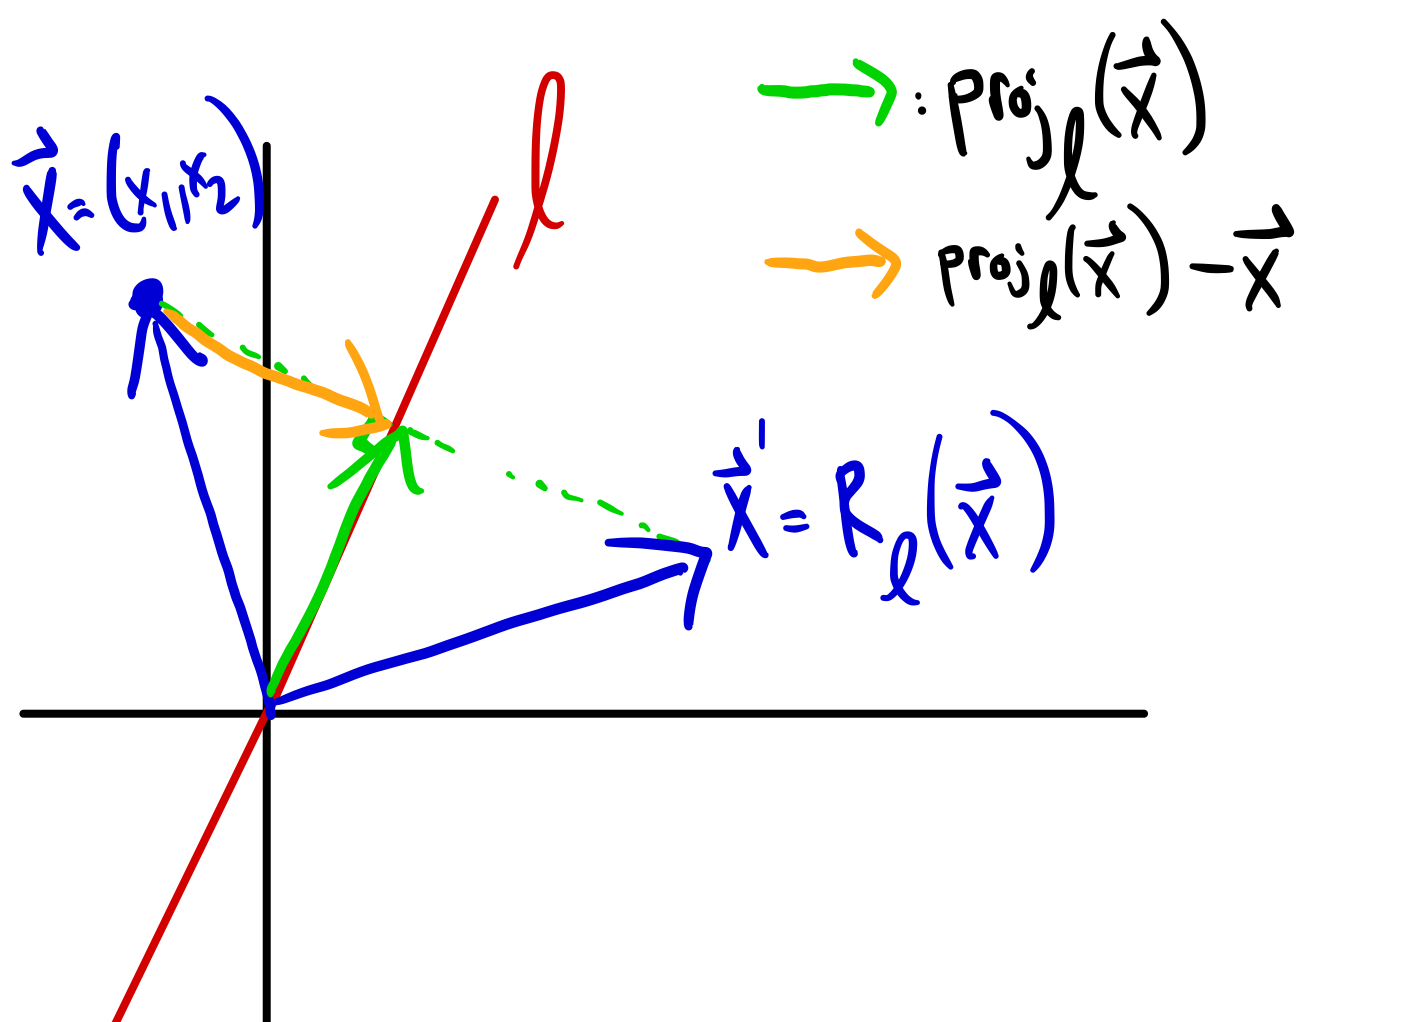
\includegraphics[width=3in]{Images/Reflection}
%\]
%\bpause 
%As the diagram illustrates, we have 
%\[
%R_\ell(\boldx)=\boldx+2(\proj{\boldx}{\ell}-\boldx)=2\proj{\boldx}{\ell}-\boldx=(2T_\ell-I_{\R^2})(\boldx),
%\]
%where $T_\ell$ is orthogonal projection onto $\ell$. 
%\end{frame}
%\begin{frame}{Reflection in $\R^2$}
%\[
%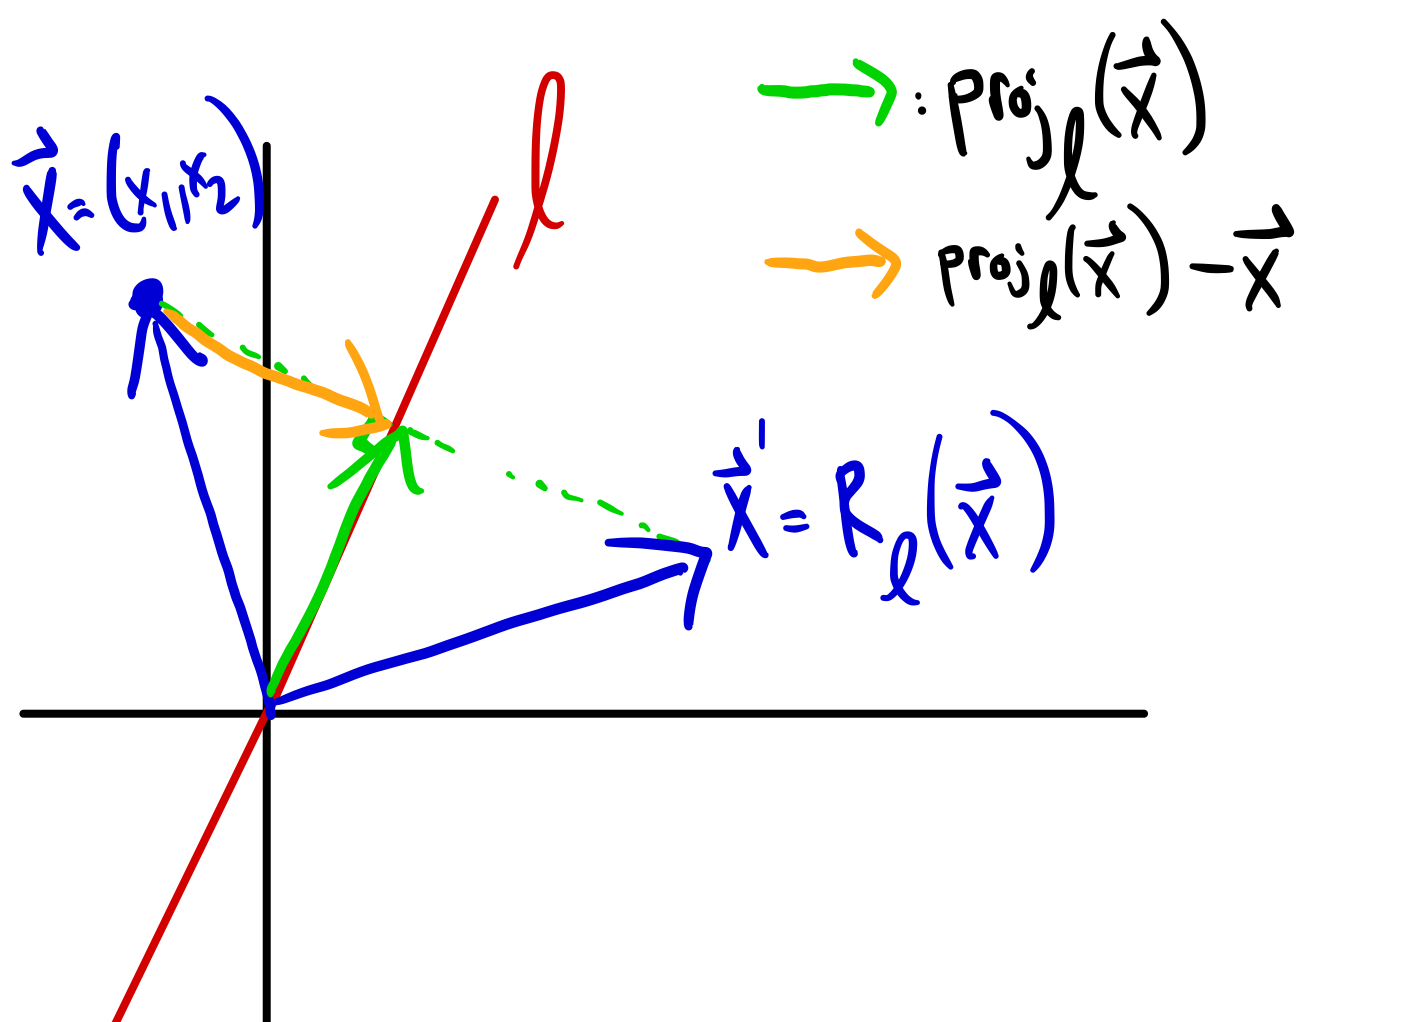
\includegraphics[width=.75in]{Images/Reflection}
%\]
%As the diagram illustrates, we have 
%\[
%R_\ell(\boldx)=\boldx+2(\proj{\boldx}{\ell}-\boldx)=2\proj{\boldx}{\ell}-\boldx=(2T_\ell-I_{\R^2})(\boldx),
%\]
%where $T_\ell$ is orthogonal projection onto $\ell$. 
%\bpause
%Write $\ell=\Span\{(y_1,y_2)\}$ for some vector $\boldy=(y_1,y_2)$. Then using our result about orthogonal projections, we have 
%\[
%R_{\ell}(x_1,x_2)=(2T_{\ell}-I_{\R^2})(x_1,x_2)=\left(\frac{2}{y_1^2+y_2^2}\begin{bmatrix}
%y_1^2&y_1y_2\\
%y_1y_2&y_2^2
%\end{bmatrix}-\begin{bmatrix}
%1&0\\
%0&1
%\end{bmatrix}\right) \begin{bmatrix}
%x_1\\ x_2
%\end{bmatrix}.
%\]
%\pause 
%This shows that $R_\ell=T_A$, where 
%\[
%A=\frac{2}{y_1^2+y_2^2}\begin{bmatrix}
%y_1^2&y_1y_2\\
%y_1y_2&y_2^2
%\end{bmatrix}-\begin{bmatrix}
%1&0\\
%0&1
%\end{bmatrix}=\frac{1}{y_1^2+y_2^2}\begin{bmatrix}
%y_1^2-y_2^2&2y_1y_2\\
%2y_1y_2&-y_1^2+y_2^2
%\end{bmatrix} .
%\]
%In particular, reflection through lines passing through the origin is linear!
%\bpause Note further, that if we let $\phi$ be the angle between $\boldy=(y_1,y_2)$ and $(1,0)$, then 
%\[
%A=\begin{bmatrix}\cos 2\phi&\sin 2\phi\\
%\sin 2\phi&-\cos 2 \phi
%\end{bmatrix}
%\]
%\end{frame} 
\begin{frame}{Exotic example: \alert{shift transformations}}
 Let $V=\R^\infty$, the vector space of all infinite sequences. 
 
 The {\bf left-shift transformation}, denoted $T_\ell$ is the function $T_\ell\colon \R^\infty\rightarrow\R^\infty$ defined as 
 \[
 T_\ell\left( (a_1,a_2,a_3,\dots)\right)=(a_2,a_3,\dots).
 \]
 
 The {\bf right-shift transformation}, denoted $T_r$ is the function $T_r\colon \R^\infty\rightarrow\R^\infty$ defined as 
 \[
 T_r\left( (a_1,a_2,a_3,\dots)\right)=(0,a_1,a_2,a_3,\dots).
 \]
 \pause
 In other words, $T_\ell$ takes an input sequence and returns as an output the sequence obtained by shifting all terms one to the left; $T_r$ takes an input sequence and returns as an output the sequence obtained by shifting all terms one to the right and setting the first term equal to 0. 
 \bpause
 \alert{Claim}: $T_\ell$ and $T_r$ are both linear transformations.
 \begin{proof}
 Exercise.
 \end{proof}
\end{frame}
\begin{frame}{Exotic example: \alert{differentiaton}}
Let $V=C^\infty(\R)$, the vector space of all infinitely differentiable functions on $\R$. 
\bspace
Define $T\colon C^\infty(\R)\rightarrow C^\infty(\R)$ by $T(f)=f'$. 
\bspace
In other words, $T$ takes as an input a function $f$, and returns as an output its derivative function $f'$. 
\bpause
\alert{Claim}: $T$ is a linear transformation. 
\pause \begin{proof}
We must show $T(cf+dg)=cT(f)+dT(g)$ for any scalars $c,d\in\R$ and any functions $f, g\in C^\infty(\R)$. 
\bpause
This follows easily from certain properties of the derivative: 
\begin{align*}
T(cf+dg)&=(cf+dg)' &\text{(def. of $T$)}\\
&=(cf)'+(dg)'&\text{(addition prop. of derivative)}\\
&=cf'+dg' &\text{(scalar prop. of derivative)}\\
&=cT(f)+dT(g) &\text{(def. of $T$)}
\end{align*}
\end{proof}
\end{frame}
%\begin{frame}{More examples}
%\footnotesize
%\bb
%\pause\ii Let $V=P_n$ and $W=P_{n+1}$, the function
%\begin{eqnarray*}
%T\colon P_n&\rightarrow& P_{n+1}\\
%p=p(x)\in P_{n}&\mapsto& T(p):=x\cdot p(x)
%\end{eqnarray*}
%is a linear transformation. 
%\pause\ii Let $V=M_{mn}$, $W=M_{nm}$. The function 
%\begin{eqnarray*}
%T\colon M_{mn}&\rightarrow& M_{nm}\\
%A\in M_{mn}&\mapsto&T(A):=A^T
%\end{eqnarray*}
%is a linear transformation. 
%\pause\ii Let $V=C^1(-\infty,\infty)$, $W=C(-\infty,\infty)$. The function 
%\begin{eqnarray*}
%T\colon C^1(-\infty,\infty)&\rightarrow& C(-\infty,\infty)\\
%f\in C^1(-\infty,\infty)&\mapsto& T(f):=f'
%\end{eqnarray*}
%is a linear transformation. 
%\bpause
%More generally, taking $f$ to its $n$-th derivative $f^{(n)}$ is a linear transformation for any $n$ thanks to the sum and scalar multiplication rules of differentiation! This property is very important in the theory of linear differential equations. 
%\ee
%\end{frame}
%\begin{frame}{Null space and range}
%\begin{definition}
%Let $V$ and $W$ be vector spaces, and $T\colon V\rightarrow W$ a linear transformation. We define
%\begin{eqnarray*}
%\NS(T)&:=&\{\boldv\in V\colon T(\boldv)=\boldzero_W\}\subseteq V\\
%\range(T)&:=&\{\boldw\in W\colon \boldw=T(\boldv)\text{ for some } \boldv\in V\}\subseteq W
%\end{eqnarray*}
%\end{definition}
%\pause
%\alert{Comments}.
%\bb
%\ii In the literature  $\NS(T)$ is also called the {\bf kernel} of $T$, denoted $\ker(T)$. I'll just stick to $\NS(T)$. 
%\pause\ii Both $\NS(T)$ and $\range(T)$ are indeed \alert{subspaces}. Note that they live in different spaces: $\NS(T)\subseteq V$ and $\range(T)\subseteq W$.  
%\pause\ii We define $\nullity(T)=\dim(\NS(T))$ and $\rank(T)=\dim(\range(T))$.
%\pause
%\ii When we are in the special case where $T_A\colon \R^n\rightarrow \R^m$ for some matrix $A\in M_{mn}$, it is easy to see that $\NS(T_A)=\NS(A)$ and $\range(T_A)=\CS(A)$.     
%\ee
%\end{frame}
%\begin{frame}{Proof that $\range(T)$ is a subspace}
%\footnotesize
%We continue to assume $T\colon V\rightarrow W$ is a linear transformation. Let's show $\range(T)=\{\boldw\in W\colon \boldw=T(\boldv)\text{ for some } \boldv\in V\}$ is a subspace. 
%\bb[(i)]
%\pause\ii We must show $\boldzero_W\in \range(T)$. But $\boldzero_W=T(\boldzero_V)$. Thus there is a $\boldv\in V$ with $T(\boldv)=\boldzero_W$, which proves that $\boldzero_W\in\range(T)$. 
%\pause\ii Suppose $\boldw_1,\boldw_2\in \range(T)$. This means there are $\boldv_1, \boldv_2\in V$ such that $T(\boldv_i)=\boldw_i$ for $i=1,2$. We must show $\boldw=\boldw_1+\boldw_2\in\range(T)$.  
%\bpause 
%Set $\boldv=\boldv_1+\boldv_2$. Then
%\begin{eqnarray*}
%T(\boldv)&=&T(\boldv_1+\boldv_2)\\
%&=&T(\boldv_1)+T(\boldv_2) \ \text{ (since $T$ is a linear transformation)}\\
%&=&\boldw_1+\boldw_2=\boldw.
%\end{eqnarray*} 
%Since we have provided a $\boldv$ with $T(\boldv)=\boldw_1+\boldw_2$, we see that $\boldw_1+\boldw_2\in\range(T)$. 
%\pause\ii Suppose $\boldw\in\range(T)$. Then there is a $\boldv\in V$ with $T(\boldv)=\boldw$. Then $T(k\boldv)=kT(\boldv)=k\boldw$, showing $k\boldw\in\range(T)$.  
%\ee
%\end{frame}
%\begin{frame}{Example: orthogonal projection}
% Let $(V, \angvec{\ , })$ be an inner product space, and let $W\subseteq V$ be a \alert{finite-dimensional} subspace. We showed in a homework exercise that the orthogonal projection map: 
% \begin{align*}
% \text{proj}_W\colon V&\rightarrow V\\
% \boldv&\mapsto \proj{\boldv}{W}
% \end{align*} 
% satisfies $\proj{c_1\boldv_1+c_2\boldv_2}{W}=c_1\proj{\boldv_1}{W}+c_2\proj{\boldv_2}{W}$. 
% \bpause 
% Thus orthogonal projection defines a linear transformation from $V$ to $V$. 
%\bpause
%\alert{Null space}. We showed in homework that $\proj{\boldv}{W}=\boldzero$ if and only if $\boldv\in W^\perp$. Thus 
%\[
%\NS(\text{proj}_W)=W^\perp.
%\]
%\bpause
%\alert{Range}.  It is easy to see that $\range(\text{proj}_W)=W$. Indeed, we have $\proj{\boldv}{W}\subseteq W$ by definition. Going the other way, given any $\boldw\in W$, we have $\proj{\boldw}{W}=\boldw$. Thus $W\subseteq \range(\text{proj}_W)$. 
%\end{frame} 
%
%\begin{frame}
%\begin{theorem}[Rank-nullity theorem]
%Let $V$ and $W$ be spaces, $T\colon V\rightarrow W$ a linear transformation. Suppose further that $V$ is \alert{finite-dimensional}. Then 
%\[
%\dim(V)=\dim(\NS(T))+\dim(\range(T).
%\]
%\end{theorem}
%\pause
%\begin{proof}
%Let $\dim V=n$. Since $V$ is finite-dimensional and $\NS(T)\subseteq V$, it follows that $\NS(T)$ is finite-dimensional. 
%\\
%\pause Let $S=\{\boldv_1,\boldv_2,\dots, \boldv_r\}$ be a basis of $\NS(T)$; \alert{extend} this basis to a full basis $\{\boldv_1,\boldv_2,\dots, \boldv_r, \boldu_{1},\dots \boldu_{n-r}\}$ of $V$. 
%\\
%\pause Claim: $S'=\{T(\boldu_{1}),\dots, T(\boldu_{n-r})\}$ is a basis of $\range(T)$. If this is true we are done, since we have $\dim(\NS(T))=\#S=r$ and $\dim(\range(T))=\#S'=n-r$,  and thus 
%\[
%\dim(V)=n=r+(n-r)=\dim(\NS(T))+\dim(\range(T).
%\]
%\pause Now ask your professor to prove the claim. 
%\end{proof}
%\end{frame}
%\begin{frame}{Linear transformations and bases}
%\begin{theorem}
%Let $S=\{\boldv_1,\dots,\boldv_n\}$ be a basis for $V$, and let $W$ be any space. 
%\bb[(a)]
%\ii Given any choice of $n$ elements $\boldw_1,\boldw_2,\dots, \boldw_n\in W$ there is a \alert{unique} linear transformation $T\colon V\rightarrow W$ such that $T(\boldv_i)=\boldw_i$. 
%\ii Given linear transformations $T_1,T_2\colon V\rightarrow W$, $T_1=T_2$ if and only if $T_1(\boldv_i)=T_2(\boldv_i)$ for $1\leq i\leq n$.  
%\ee
%\end{theorem}
%\pause
%This is an extremely useful theorem as it allows us, given a basis $S$ of $V$, to 
%\bb[(i)]
%\ii easily define linear transformations simply by declaring where $\boldv_i$ gets sent for each $i$, and 
%\pause \ii easily check whether two linear transformations are equal simply by checking that they agree on the basis elements $\boldv_i$. 
%\ee
%\end{frame}
%\begin{frame}{Transformations of $\R^n$}
%An important corollary of this theorem is the fact that \alert{every} linear transformation $T\colon\R^n\rightarrow\R^m$ between is given by a matrix: that is, $T=T_A$ for some $m\times n$ matrix $A$. 
%\bspace 
%Indeed, given such a $T$, let $A$ be the matrix whose $j$-th column is $\boldc_j=T(\bolde_j)$, where $\bolde_j$ is the $j$-th element of the standard basis of $\R^n$. I claim $T=T_A$. 
%\pause
%\begin{proof}
%According to the theorem, I only need to show that $T$ and $T_A$ agree on any basis of $\R^n$. Let's take the standard basis $B=\{\bolde_1,\dots,\bolde_n\}$. 
%
%\pause Then 
%\begin{align*}
%T_A(\bolde_j)&=A\bolde_j &\text{(def. of $T_A$) }\\
%&=\boldc_j &\text{(column expansion)}\\
%&=T(\bolde_j) &\text{(def. of $A$)}
%\end{align*}
%We've shown that $T_A(\bolde_j)=T(\bolde_j)$ for all $\bolde_j\in B$. The theorem implies $T=T_A$. 
%\end{proof}
%\end{frame}
%\begin{frame}{Example: rotations}
%Fix an angle $\theta$ and consider the map $T_\theta\colon\R^2\rightarrow\R^2$ that takes a vector $\boldx$ and maps it to the vector $\boldy=T_\theta(\boldx)$ you get by rotating $\boldx$ by $\theta$, taking counterclockwise to be the positive direction. We call this map a \alert{rotation} by $\theta$. 
%\bpause
%Take for granted for the time being that $T_\theta$ is in fact a linear transformation (not totally obvious). Find the matrix $A_\theta$ that represents this linear transformation. 
%\begin{bsolution}
%According to the previous slide we have 
%\[
%A_\theta=\begin{bmatrix}\vert &\vert\\ T_\theta(\bolde_1)&T_\theta(\bolde_2)\\ \vert &\vert \end{bmatrix},
%\]
%where $\bolde_1=\begin{bmatrix}
%1\\0
%\end{bmatrix} $ and $ \bolde_2=\begin{bmatrix}
%0\\1
%\end{bmatrix}$, as usual.  \pause A simple drawing on the unit circle tells us what happens to these vectors when we rotate them by $\theta$. We get:
%\[
%T_\theta(\bolde_1)=\begin{bmatrix}
%\cos(\theta)\\ \sin(\theta)
%\end{bmatrix}, T_\theta(\bolde_2)=\begin{bmatrix}
%-\sin(\theta)\\ \cos(\theta)
%\end{bmatrix}
%\]
%Thus 
%\[
%A_\theta=\begin{bmatrix}
%\cos(\theta)&-\sin(\theta)\\ \sin(\theta) &\cos(\theta)
%\end{bmatrix}
%\]
%We call this a \alert{rotation matrix}.  
%\end{bsolution} 
%\end{frame}
%\begin{frame}{Projection onto a line in $\R^n$, $n=2,3$}
%Let $V=\R^n$ for $n=2$ or $n=3$, and let $\ell\subseteq V$ be a line passing through the origin. Define $T_\ell$ to be the transformation that takes a vector $\boldx$ and returns its \alert{orthogonal projection} $\proj{\boldx}{\ell}$ onto $\ell$: i.e., we define $T_\ell(\boldx)=\proj{\boldx}{\ell}$. 
%\bpause
%We have $\ell=\Span\{\boldy\}$ for some vector $\boldy\in \R^n$. In multivariable calculus we derive a dot product formula orthogonal projection: namely, $\proj{\boldx}{\ell}=(\frac{\boldx\cdot\boldy}{\boldy\cdot\boldy})\boldy$. We can use this formula to identify $T_\ell=T_A$ for a matrix $A\in M_{nn}$. We treat $n=2, 3$ separately.  
%\bpause
%{\color{blue} Case $n=2$}. Let $\boldy=(y_1,y_2)$. For $(x_1, x_2)$ we have 
%\[
%\proj{(x_1,x_2)}{\ell}=\frac{y_1x_1+y_2x_2}{y_1^2+y_2^2}(y_1,y_2)=\frac{1}{y_1^2+y_2^2}\begin{bmatrix}
%y_1^2&y_1y_2\\
%y_1y_2&y_2^2
%\end{bmatrix} \begin{bmatrix}
%x_1\\ x_2
%\end{bmatrix} 
%\]
%\bpause
%{\color{blue} Case $n=3$}. Let $\boldy=(y_1,y_2,y_3)$. For $(x_1, x_2,x_3)$ we have 
%\[
%\proj{(x_1,x_2,x_3)}{\ell}=\frac{y_1x_1+y_2x_2+y_3x_3}{y_1^2+y_2^2+y_3^2}(y_1,y_2,y_3)=\frac{1}{y_1^2+y_2^2+y_3^2}\begin{bmatrix}
%y_1^2&y_1y_2&y_1y_3\\
%y_1y_2&y_2^2&y_2y_3\\
%y_1y_3&y_2y_3&y_3^2
%\end{bmatrix} \begin{bmatrix}
%x_1\\ x_2\\x_3
%\end{bmatrix} 
%\]
%\pause 
%Thus $T_\ell=T_A$ where $A=\frac{1}{y_1^2+y_2^2}\begin{bmatrix}
%y_1^2&y_1y_2\\
%y_1y_2&y_2^2
%\end{bmatrix}$ in the $n=2$ case, and $A=\frac{1}{y_1^2+y_2^2+y_3^2}\begin{bmatrix}
%y_1^2&y_1y_2&y_1y_3\\
%y_1y_2&y_2^2&y_2y_3\\
%y_1y_3&y_2y_3&y_3^2
%\end{bmatrix}$ in the $n=3$ case.
%\end{frame} 
%\begin{frame}{Reflection in $\R^2$}
%Let $V=\R^2$. Given an arbitrary line $\ell$ passing through the origin, let $R_\ell$ be the transformation that maps a vector $\boldx$ to its reflection $\boldx'=R_\ell(\boldx)$ across $\ell$. 
%\[
%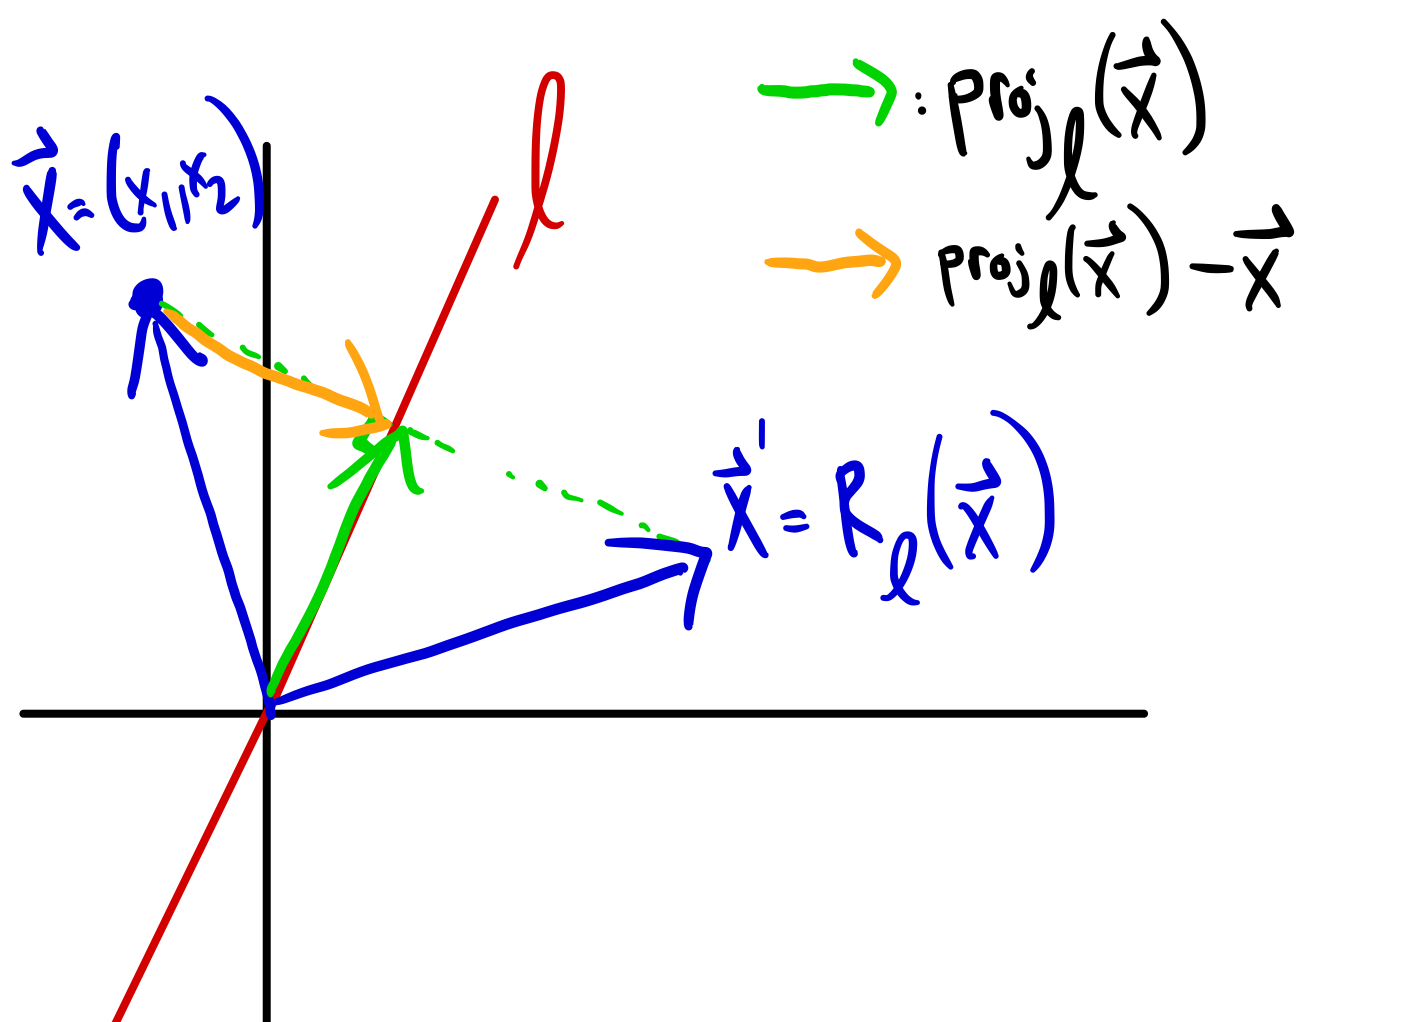
\includegraphics[width=3in]{Images/Reflection}
%\]
%\bpause 
%As the diagram illustrates, we have 
%\[
%R_\ell(\boldx)=\boldx+2(\proj{\boldx}{\ell}-\boldx)=2\proj{\boldx}{\ell}-\boldx=(2T_\ell-I_{\R^2})(\boldx),
%\]
%where $T_\ell$ is orthogonal projection onto $\ell$. 
%\end{frame}
%\begin{frame}{Reflection in $\R^2$}
%\[
%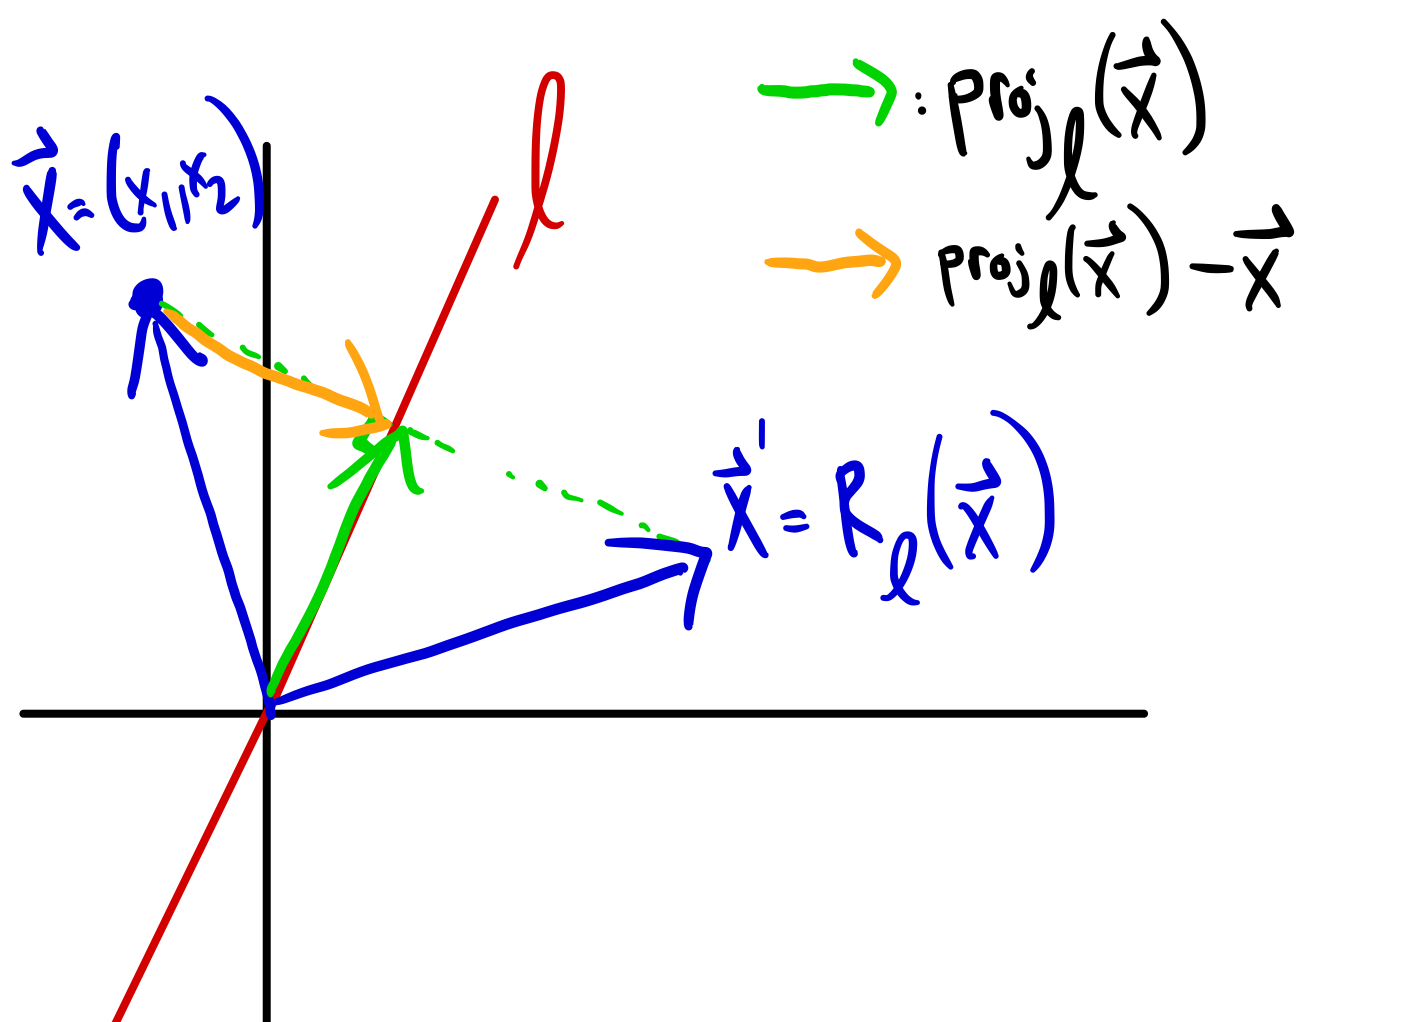
\includegraphics[width=.75in]{Images/Reflection}
%\]
%As the diagram illustrates, we have 
%\[
%R_\ell(\boldx)=\boldx+2(\proj{\boldx}{\ell}-\boldx)=2\proj{\boldx}{\ell}-\boldx=(2T_\ell-I_{\R^2})(\boldx),
%\]
%where $T_\ell$ is orthogonal projection onto $\ell$. 
%\bpause
%Write $\ell=\Span\{(y_1,y_2)\}$ for some vector $\boldy=(y_1,y_2)$. Then using our result about orthogonal projections, we have 
%\[
%R_{\ell}(x_1,x_2)=(2T_{\ell}-I_{\R^2})(x_1,x_2)=\left(\frac{2}{y_1^2+y_2^2}\begin{bmatrix}
%y_1^2&y_1y_2\\
%y_1y_2&y_2^2
%\end{bmatrix}-\begin{bmatrix}
%1&0\\
%0&1
%\end{bmatrix}\right) \begin{bmatrix}
%x_1\\ x_2
%\end{bmatrix}.
%\]
%\pause 
%This shows that $R_\ell=T_A$, where 
%\[
%A=\frac{2}{y_1^2+y_2^2}\begin{bmatrix}
%y_1^2&y_1y_2\\
%y_1y_2&y_2^2
%\end{bmatrix}-\begin{bmatrix}
%1&0\\
%0&1
%\end{bmatrix}=\frac{1}{y_1^2+y_2^2}\begin{bmatrix}
%y_1^2-y_2^2&2y_1y_2\\
%2y_1y_2&-y_1^2+y_2^2
%\end{bmatrix} .
%\]
%In particular, reflection through lines passing through the origin is linear!
%\bpause Note further, that if we let $\phi$ be the angle between $\boldy=(y_1,y_2)$ and $(1,0)$, then 
%\[
%A=\begin{bmatrix}\cos 2\phi&\sin 2\phi\\
%\sin 2\phi&-\cos 2 \phi
%\end{bmatrix}
%\]
%\end{frame} 
%\begin{frame}{Example: orthogonal projection in $\R^2$}
% Consider $\R^3$ with the dot product, and let $W$ be the plane orthogonal to the vector $\boldn=(a,b,c)$. For $\boldx\in\R^3$, define $T(\boldx)$ to be the orthogonal projection of 
% 
%  \bpause 
% We derived a formula for $A$ in terms of $a,b,c$ earlier. We do so again, this time column by column: 
% \pause
% \begin{align*}
% \proj{\bolde_1}{W}&=\bolde_1-\proj{\bolde_1}{W^\perp}=\bolde_1-\frac{\bolde_1\cdot \boldn}{\boldn\cdot\boldn}\boldn=\frac{1}{a^2+b^2+c^2}\colvec{b^2+c^2\\ -ab\\ -ac}\\
% \proj{\bolde_2}{W}&=\bolde_2-\proj{\bolde_2}{W^\perp}=\bolde_2-\frac{\bolde_2\cdot \boldn}{\boldn\cdot\boldn}\boldn=\frac{1}{a^2+b^2+c^2}\colvec{-ab\\ a^2+c^2\\ -bc}\\
% \proj{\bolde_3}{W}&=\bolde_3-\proj{\bolde_3}{W^\perp}=\bolde_3-\frac{\bolde_3\cdot \boldn}{\boldn\cdot\boldn}\boldn=\frac{1}{a^2+b^2+c^2}\colvec{-ac\\ -bc\\ a^2+b^2}
% \end{align*} 
% \pause Thus $\text{proj}_W=T_A$, where $A=\frac{1}{a^2+b^2+c^2}\begin{bmatrix}
%  b^2+c^2& -ab&-ac\\
%  -ab&a^2+c^2&-bc\\
%  -ac&-bc&a^2+b^2
% \end{bmatrix} 
% $
%\end{frame} 
%\begin{frame}{Example: orthogonal projection in $\R^3$}
% Consider $\R^3$ with the dot product, and let $W$ be the plane orthogonal to the vector $\boldn=(a,b,c)$. Since $\text{proj}_W\colon\R^3\rightarrow \R^3$ is a linear transformation of $\R^3$, we must have $\text{proj}_W=T_A$ for some $A\in M_{33}$. 
% \bpause 
% We derived a formula for $A$ in terms of $a,b,c$ earlier. We do so again, this time column by column: 
% \pause
% \begin{align*}
% \proj{\bolde_1}{W}&=\bolde_1-\proj{\bolde_1}{W^\perp}=\bolde_1-\frac{\bolde_1\cdot \boldn}{\boldn\cdot\boldn}\boldn=\frac{1}{a^2+b^2+c^2}\colvec{b^2+c^2\\ -ab\\ -ac}\\
% \proj{\bolde_2}{W}&=\bolde_2-\proj{\bolde_2}{W^\perp}=\bolde_2-\frac{\bolde_2\cdot \boldn}{\boldn\cdot\boldn}\boldn=\frac{1}{a^2+b^2+c^2}\colvec{-ab\\ a^2+c^2\\ -bc}\\
% \proj{\bolde_3}{W}&=\bolde_3-\proj{\bolde_3}{W^\perp}=\bolde_3-\frac{\bolde_3\cdot \boldn}{\boldn\cdot\boldn}\boldn=\frac{1}{a^2+b^2+c^2}\colvec{-ac\\ -bc\\ a^2+b^2}
% \end{align*} 
% \pause Thus $\text{proj}_W=T_A$, where $A=\frac{1}{a^2+b^2+c^2}\begin{bmatrix}
%  b^2+c^2& -ab&-ac\\
%  -ab&a^2+c^2&-bc\\
%  -ac&-bc&a^2+b^2
% \end{bmatrix} 
% $
%\end{frame} 

\subsection{Subspaces}\label{ss:subspace}
%\begin{frame}<beamer>
%             \frametitle{Outline}
%             \tableofcontents[currentsection,currentsubsection]
%\end{frame}      
\begin{frame}{\ref{s:vectorspace}.\ref{ss:subspace}: executive summary}
\alert{Definitions:} subspace, linear combination, span, polynomial spaces $P$ and $P_n$, $\NS T$, $\range T$. 
\bspace
\alert{Procedures:} proving something is/isn't a subspace; computing the span of a set of vectors, computing $\NS T$ and $\range T$ for a linear transformation. 
\bspace
\alert{Theorems:} intersection of subspaces is a subspace, $\Span(\{\boldv_1,\boldv_2,\dots\})$ is a subspace, $\NS T$ is a subspace, $\range T$ is a subspace.
\end{frame}
\begin{frame}{\ref{s:vectorspace}.\ref{ss:subspace}: subspaces}\footnotesize
\begin{definition}
Let $V$ be a vector space. A subset $W\subseteq V$ is a {\bf subspace} of $V$ if
\bb[(i)]
\ii $\boldzero\in W$,
\ii $\boldw_1, \boldw_2\in W\Rightarrow \boldw_1+\boldw_2\in W$, (i.e., $W$ is {\bf closed under addition}),
\ii $\boldw\in W\Rightarrow k\boldw\in W$ for all $k\in\R$ (i.e., $W$ is {\bf closed under scalar multiplication}). 
\ee 
\end{definition}
\pause
\alert{Comments}\\
(1) You may see slightly different definitions for subspace in the literature: e.g., some define a subspace to be a subset $W\subseteq  V$ which, under the operations of addition and scalar multiplication of $V$, is itself a vector space. I prefer mine as it gives you a hands-on method of deciding whether a given subset of $W\subseteq V$ is in fact a sub{\em space} of $V$: namely, determine whether each of properties (i)-(iii) hold for $W$.
\bpause
(2) Each of properties (ii) and (iii) is stated as an \alert{implication}. Thus when verifying these, as always we assume the antecedent and prove the consequent.     
\end{frame}
\begin{frame}{Example}
\footnotesize
Let $V=\R^2$ and let $W\subseteq V$ be the subset $W=\{(t,t)\in\R^2
\colon t\in\R\}$. We claim $W$ is a subspace. 
\pause \begin{proof}
We must show properties (i)-(iii) hold for $W$. 
\bpause
(i) The zero element of $V$ is $\boldzero=(0,0)$, which is certainly of the form $(t,t)$. Thus $\boldzero\in W$. 
\bpause
(ii) We must prove the implication $\boldw_1, \boldw_2\in W\Rightarrow \boldw_1+\boldw_2\in W$. 
\begin{eqnarray*}
\pause\boldw_1,\boldw_2\in W&\Rightarrow& \boldw_1=(t,t), \boldw_2=(s,s) \text{ for some $t,s\in\R$}\\
\pause&\Rightarrow&\boldw_1+\boldw_2=(t+s,t+s) \\
\pause&\Rightarrow&\boldw_1+\boldw_2\in W.
\end{eqnarray*}
\pause
(iii) We must prove the implication $\boldw\in W\Rightarrow k\boldw\in W$. 
\begin{eqnarray*}
\pause \boldw\in W&\Rightarrow& \boldw=(t,t)\\
\pause&\Rightarrow& k\boldw=(kt,kt)\\
\pause&\Rightarrow& k\boldw\in W
\end{eqnarray*}
\end{proof}
\end{frame}
\begin{frame}{Example}
\footnotesize
Let $V=\R^n$, and treat elements of $V$ as \alert{column vectors}. Fix a vector $\boldv_0\in V$. Let $W\subseteq V$ be the subset $W=\{\boldw\in \R^n\colon \boldv_0^T\boldw=0\}$. We claim $W$ is a subspace. 
\pause \begin{proof}
We must show properties (i)-(iii) hold for $W$. 
\bpause
(i) The zero element of $V$ is $\boldzero=\colvec{0\\ \vdots\\ 0}$. Clearly $\boldv_0^T\boldzero=0$. Thus $\boldzero\in W$. 
\bpause
(ii) We must prove the implication $\boldw_1, \boldw_2\in W\Rightarrow \boldw_1+\boldw_2\in W$. 
\begin{eqnarray*}
\pause\boldw_1,\boldw_2\in W&\Rightarrow& \boldv_0^T\boldw_1=0,\boldv_0^T\boldw_2=0 \\
\pause&\Rightarrow&\boldv_0^T(\boldw_1+\boldw_2)=\boldv_0^T\boldw_1+\boldv_0^T\boldw_2=0+0=0\\
\pause&\Rightarrow& \boldw_1+\boldw_2\in W.
\end{eqnarray*}
\pause
(iii) We must prove the implication $\boldw\in W\Rightarrow k\boldw\in W$. 
\begin{eqnarray*}
\pause\boldw\in W&\Rightarrow& \boldv_0^T\boldw=0\\
\pause&\Rightarrow& \boldv_0^T(k\boldw)=k\boldv_0^T\boldw=k0=0\\
\pause&\Rightarrow& k\boldw\in W
\end{eqnarray*}
\end{proof}
\end{frame}
\begin{frame}{Lines and planes}
Recall that a line in $\R^2$ \alert{containing the origin $(0,0)$} can be expressed as the set of solutions $(x_1,x_2)\in\R^2$ to an equation of the form
\[
ax_1+bx_2=0, \text{ or } \colvec{a\\b}^T\colvec{x_1\\ x_2}=0
\]

Similarly, a plane in $\R^3$ \alert{containing the origin $(0,0,0)$} can be expressed as the the set of solutions $(x_1,x_2,x_3)$ to an equation of the form 
\[
ax_1+bx_2+cx_3=0, \text{ or } \colvec{a\\b\\c}^T\colvec{x_1\\x_2\\x_3}=0.
\]
\pause By the previous example we see that lines in $\R^2$ containing the origin are subspaces, as are planes in $\R^3$ containing the origin! Both can be expressed in the form $W=\left\{\boldx\colon \boldv_0^T\boldx=0\right\}$: take $\boldv_0=(a,b)$ in the first case, and $\boldv_0=(a,b,c)$ in the second. 
\bpause
On the other hand, a line or place that does \alert{not} contain the origin is not a subspace, since it does not contain $\boldzero$. 
\bpause
We will revisit this example after defining the dot product on $\R^n$. 
\end{frame}
%\begin{frame}{Subspaces of $F(-\infty,\infty)$}
%\footnotesize
%In the following you can replace $(-\infty,\infty)$ with $X$ for any subinterval of $\R$. 
%\bspace
%Let $V=F(-\infty,\infty)$, the vector space of all functions on the real line. We can define the following natural subsets of $V$. 
%\[
%\begin{array}{ccl}
%V&=&F(-\infty,\infty)=(\text{set of all functions } f\colon (-\infty,\infty)\rightarrow\R)\\
%\rotatebox{90}{$\subseteq$}& \\
%C(-\infty,\infty)&=&\{f\in V\colon f \text{ continuous}\}\\
%\rotatebox{90}{$\subseteq$}& \\
%C^1(-\infty,\infty)&=&\{f\in V\colon f' \text{ exists and is cont.}\}\\
%\rotatebox{90}{$\subseteq$}& \\
%C^2(-\infty,\infty)&=&\{f\in V\colon f', f'' \text{ exist and are cont.}\}\\
%\rotatebox{90}{$\subseteq$}& \\
%\vdots \\
%C^\infty(-\infty,\infty)&=&\{f\in V \colon f^{(n)} \text{ exists for all $n$}\}
%\end{array}
%\]
%\pause In fact these are all sub{\em spaces} of $V$. Proof: (i) the zero function, $h(x)=0$ for all $x$, is $\infty$-differentiable, and thus is an element of each of these sets; (ii)-(iii) these sets being closed under addition and scalar mult. is a consequence of calculus results about sums and scalar multiples of continuous/differentiable functions.  
%\end{frame}
\begin{frame}{Polynomials}\footnotesize
Recall that a {\bf polynomial} is a function that can be written in the form $f(x)=\anpoly$, where $a_i\in\R$ are fixed constants and $a_n\ne 0$. We call $n$ the {\bf degree} of such a function, denoted $\deg f=n$. 
\bpause
Let $P$ be the set of all polynomial functions, and let $P_n=\{f\colon f(x)=\anpoly, a_i\in\R \}$ be the set of all polynomials of degree \alert{at most} $n$. 

We have the set inclusions $P_n\subset P\subset C^\infty(X)$, where $X$ is any nontrivial interval. (The second inclusion holds since any polynomial is infinitely differentiable on any interval. )
\bpause
It is easy to see that in fact $P_n$ is a \alert{subspace} of $P$, and $P$ is a \alert{subspace} of $C^\infty(X)$. 
Indeed $P_n$ and $P$ both contain the zero polynomial $f(x)=0=0x^n+0x^{n-1}+\cdots 0x+0$, which is the same thing as the zero function $0_X=\boldzero$. Furthermore, sums and scalar multiples of polynomials (resp. of polynomials of at most degree $n$) are polynomials (resp. polynomials of at most degree $n$). 
\bpause
\alert{Important:} a fact we will make use of all the time is that for two polynomials 
\[\begin{array}{l}
f(x)=\anpoly, \ a_n\ne 0 \\
g(x)=\bmpoly, \ b_m\ne 0
\end{array}
\] 
we have $f(x)=g(x)$ if and only if (1) n=m, and (2) $a_i=b_i$ for all $0\leq i\leq n$. 
\end{frame}
\begin{frame}{Intersections and unions}
\begin{theorem}
Let $V$ be a vector space, and suppose $W_1,W_2,\dots, W_r$ are each subspaces of $V$. Then the intersection $W=W_1\cap W_2\cdots \cap W_r$ is a subspace of $V$. 
\end{theorem}
\pause
\alert{Comment}. Thus intersections of subspaces are subspaces. The same is not true of \alert{unions}. 
\bpause
For example, take $V=\R^2$, $W_1=\{(t,t)\colon t\in\R\}$ and $W_2=\{(t,-t)\colon t\in\R\}$. Then each $W_i$ is a subspace, but their union $W_1\cup W_2$ is not. Why?
\bpause
We have $\boldw_1=(1,1)\in W_1\subset W_1\cup W_2$ and $\boldw_2=(1,-1)\in W_2\subset W_1\cup W_2$, but $\boldw_1+\boldw_2=(2,0)\notin W_1\cup W_2$.  
\bpause
Note that $W_1\cup W_2$ is in fact closed under scalar multiplication. 
\end{frame}
\subsubsection*{Span}
\begin{frame}{Linear combinations and span}
Recall that a \alert{linear combination} in a vector space $V$ is a vector of the form 
\[
\boldv=k_1\boldv_1+k_2\boldv_2\cdots +k_r\boldv_r,
\] 
where $k_i\in \R$ are scalars. 
\bpause We use this notion to define the \alert{span} of a set of vectors. 
\begin{definition}
Let $V$ be a vector space, and let $S=\{\boldv_1,\boldv_2,\dots,\boldv_r\}$ be a set of vectors of $V$. The {\bf span} of $S$ is the set 
\begin{eqnarray*}
\Span(\{\boldv_1,\boldv_2,\dots,\boldv_r\})&:=&\left(\begin{array}{c} \text{the set of all linear } \\ \text{combinations of the $\boldv_i$}\end{array}\right)\\
&=&\{\boldv\in V\colon \boldv=k_1\boldv_1+k_2\boldv_2\cdots +k_r\boldv_r, \text{ for some } k_i\in\R \}.
\end{eqnarray*}
\end{definition}
\end{frame}
\begin{frame}
\begin{theorem}
Let $V$ be a vector space,  $S=\{\boldv_1,\boldv_2,\dots,\boldv_r\}$ a set of vectors of $V$, and $W=\Span(S)$. Then 
\bb[(i)]
\ii $W$ is a subspace of $V$;
\ii if $W'$ is a subspace containing all the vectors $\boldv_i$, then $W\subseteq W'$.
\ee
We paraphrase (ii) by saying $W=\Span(S)$ is the ``smallest" subspace of $V$ containing all the $\boldv_i$. 
\end{theorem}
\pause
\alert{More terminology:} in the spirit of the last theorem, given a set of vectors $S=\{\boldv_1,\dots, \boldv_r\}$, we call $W=\Span(S)$ the subspace of $V$ {\bf generated by} the vectors $\boldv_i$. Similarly, given a subspace $W$, a set $S=\{\boldv_1,\dots, \boldv_r\}$ for which $W=\Span(S)$ is called a {\bf spanning set} of $W$. 
\end{frame}
\begin{frame}{Examples}
\alert{$M_{mn}$}. Define $E_{ij}$ to be the matrix whose $(i,j)$-th entry is 1, and whose every other entry is 0. Then the set 
\[
\{ E_{ij}\colon 1\leq i\leq m, 1\leq j\leq n\}
\]
is a spanning set for $M_{mn}$. 
\bpause
\alert{$\R^n$}. In a similar vein, define $\bolde_i$ to be the $n$-tuple whose $i$-th entry is 1, and whose every other entry is 0.

Then $\{\bolde_1, \bolde_2, \dots, \bolde_n\}$ is a spanning set for $\R^n$. 
\bpause 
\alert{$P$ and $P_n$}. The set $\{1, x, x^2, \dots, \}$ is a spanning set for $P$. The set $\{1, x, x^2, \dots, x^n\}$ is a spanning set for $P_n$. 
\bpause
\alert{$\R^\infty$}. As above we can define $\bolde_i\in \R^\infty$ to be the infinite sequence whose $i$-th entry is 1, and whose every other entry is $0$. 

Note, however, that the set $\{\bolde_1, \bolde_2, \bolde_3, \dots\}$ is \alert{not} a spanning set for $\R^\infty$.
\bpause
Indeed, the sequence $(1,1,1,\dots)$ is not a (finite!) linear combination of the $\bolde_i$. 
\bpause
\alert{$\R_{>0}$} Any $a\ne 1\in \R_{>0}$ forms a spanning set for $\R_{>0}$ as a vector space. This is because scalar multiplication by $r$ in $\R_{>0}$ is defined as exponentiation. Thus $\Span(\{a\})=\{a^r\colon r\in\R\}=\R_{>0}$. The last equality holds since the exponential function $f(x)=a^x$ has range all positive reals for any base $a\ne 1$. 
\end{frame}
\begin{frame}{Example}
Let $V=P_2$ and let $S=\{p_1, p_2\}$, where $p_1(x)=x^2-1$ and $p_2(x)=x^2-x$. Show that $W=\Span(S)$ is the subspace of all polynomials $p(x)=a_2x^2+a_1x+a_0$ for which $p(1)=0$. That is:
\[
\Span(S)=\{p(x)\in P_2\colon p(1)=0\}
\]
\pause
\begin{proof}
We wish to prove a \alert{set equality}. We do so by showing the $\subseteq$ and $\supseteq$ relations separately.  (See my proof technique guide!)
\bpause 
\alert{$\subseteq$}. Note first that $p_1(1)=p_2(1)=0$. Given an element $q(x)\in \Span\left(\{p_1(x), p_2(x)\}\right)$, we have $q(x)=ap_1(x)+bp_2(x)$ for some $a, b\in \R$. But then $q(1)=ap_1(1)+bp_2(1)=0+0=0$. Thus $q(x)\in \{p(x)\colon p(1)=0\}$. 
\bpause
\alert{$\supseteq$}. Now take $p(x)=a_2x^2+a_1x+a_0\in \{p(x)\in P_2\colon p(1)=0\}$. We must find $a, b\in \R$ such that $p(x)=ap_1+bp_2$. 
\bpause Since $p(1)=0$, we have $a_2+a_1+a_0=0$. I claim $p(x)=(-a_0)p_1+(-a_1)p_2$. Indeed we have 
\[
-a_0p_1-a_1p_2=(-a_0-a_1)x^2+a_1x+a_0=a_2x^2+a_1x+a_0,
\]
since $a_2+a_1+a_0=0$. This shows that $p(x)\in\Span\left(\{p_1, p_2\}\right)$, as desired. 
\end{proof}
\end{frame}
\begin{frame}{Example}
Let $V=P_2$ and let $S=\{p_1, p_2, p_3\}$ where 
\[
p_1(x)=x^2+x+1, p_2(x)=x^2+x, p_3(x)=x^2+1.
\]
Show that $\Span(S)=P_2$. 
\pause
\begin{proof}
Again, we are tasked with showing a \alert{set equality}. 
\bspace
It is clear that $\Span(S)=\{rp_1+sp_2+tp_3\colon r,s,t\in\R\}\subseteq P_2$. 
\bspace
The harder direction is showing $P_2\subseteq \Span(S)$: i.e., given {\em any} $p(x)=a_2x^2+a_1x+a_0$ we must show there are $r,s,t\in\R$ such that $p(x)=rp_1+sp_2+tp_3$. 
\bpause 
We do so by setting up a system of equations. Combining like terms and equating coefficients in the polynomial expression $p(x)=rp_1+sp_2+tp_3$ yields the linear system 
\[
\begin{linsys}{3}
r&+&s&+&t&=&a_2\\
r&+&s&&&=&a_1\\
r&&&+&t&=&a_0
\end{linsys}
\]
\pause GE shows that the system has a solution for {\em any} choice of $a_2, a_1, a_0$: namely, $r=-a_2+a_1+a_0$, $s=a_2-a_0$, $t=a_2-a_1$. Thus given any $p(x)=a_2x^2+a_1x+a_0$, we can find $r,s,t$ such that $p=rp_1+sp_2+tp_3$, showing $P_2\subseteq \Span(S)$. 
\end{proof}
\end{frame}
\subsubsection*{Null space}

\begin{frame}{Null space of a linear transformation}
The notion of span is a useful tool for constructing subspaces inside a space $V$: given any collection $\{\boldv_1, \boldv_2, \dots, \boldv_r\}$, we now know that the set  $W=\Span(\{\boldv_1,\boldv_2,\dots, \boldv_r\})$ is guaranteed to be a subspace of $V$. 
\bpause 
The notion of a \alert{null space} of a linear transformation $T\colon V\rightarrow W$ provides another useful tool for constructing subspaces. 
\begin{definition}
The {\bf null space} of a linear transformation $T\colon V\rightarrow W$ is the set 
\[
\NS T\colon =\{\boldv\colon T(\boldv)=\boldzero_W \}.
\]
\pause 
In the special case where $T\colon \R^n\rightarrow \R^m$ and $T=T_A$, we may write $\NS A$ for $\NS T_A$: by definition this is the set 
\[
\NS A=\NS T_A=\{\boldx\in \R^n\colon A\boldx=\underset{m\times 1}{\boldzero}\}.
\]
In other words, $\NS A$ is the set of solutions to the homogenous matrix equation $A\boldx=\boldzero$, or equivalently, its associated homogenous system of equations. 
\end{definition}
\pause
As we see in the next theorem, given linear $T\colon V\rightarrow W$, its null space $\NS T$ is always a \alert{subspace} !!
\end{frame}
\begin{frame}
 \begin{theorem}[Null space theorem]
 Let $T\colon V\rightarrow W$. Then $\NS T$ is a subspace of $V$. 
 \end{theorem}
 \pause
 \begin{proof}
 \ 
 \bb[(i)]
 \ii Since $T(\boldzero_V)=\boldzero_W$, we see that $\boldzero_V\in \NS T$. 
 \pause
 \ii Suppose $\boldv_1, \boldv_2\in \NS T$. We have 
 \begin{align*}
 T(\boldv_1+\boldv_2)&=T(\boldv_1)+T(\boldv_2) &\text{($T$ is linear)}\\
 &=\boldzero_W+\boldzero_W &\text{(since $\boldv_1,\boldv_2\in\NS T$)}\\
 &=\boldzero_W.
 \end{align*}
 Thus $\boldv_1+\boldv_2\in \NS T$, proving the implication $\boldv_1,\boldv_2\in\NS T\Rightarrow \boldv_1+\boldv_2\in\NS T$. 
 \pause
 \ii Suppose $\boldv\in\NS T$. We have 
 \begin{align*}
 T(c\boldv)&=cT(\boldv) &\text{($T$ is linear)}\\
 &=c\boldzero_W &\text{(since $\boldv\in\NS T$)}\\
 &=\boldzero_W.
 \end{align*}
 This shows $c\boldv\in\NS T$, proving the implication $\boldv\in\NS T\Rightarrow c\boldv\in\NS T$. 
 \ee
  \pause Since $\NS T$ satisfies the conditions (i)-(iii), we see that it is a subspace of $V$. 

 \end{proof}
\end{frame}
\begin{frame}{Examples}
The theorem gives us a clever, indirect way of proving a subset $V'\subseteq V$ is a subspace: namely, find a linear transformation $T\colon V\rightarrow W$ for which $V'=\NS T$ !! 
\bpause
\begin{example}
The set $W\subseteq\R^3$ of all vectors $(x,y,z)$ satisfying $x+2y+3z=x-y-z=0$ is a subspace of $\R^3$. 

Indeed we have $W=\NS A$ where $A=\begin{bmatrix}
1&2&3\\
1&-1&-1
\end{bmatrix}
$.
\end{example} 
\pause
\begin{example}
The set $W=\{A\in M_{nn}\colon A^T=A\}$, consisting of all symmetric $n\times n$ matrices, is a subspace of $M_{nn}$. 

Indeed, we have $W=\NS T$, where $T\colon M_{nn}\rightarrow M_{nn}$ is the linear transformation defined as $T(A)=A^T-A$. 

(I leave it to you to show $T$ is linear.) 
\end{example}
\pause
\begin{example}
The set $W$ of all infinitely differentiable functions $f$ satisfying the differential equation $f''(x)+xf'(x)=3f(x)$ is a subspace of $C^\infty(\R)$. 

Indeed $W$ is $\NS T$, where $T\colon C^\infty(\R)\rightarrow C^\infty(\R)$ is the linear transformation defined as $T(f)=f''+xf'-3f$.

(I leave it to you to show $T$ is linear.) 

\end{example}
\end{frame}
\subsubsection*{Range of a linear transformation}
\begin{frame}{Range}
\begin{definition}
In general given a function $f\colon A\rightarrow B$ with domain $A$ and codomain $B$, its {\bf range} is the set 
\[
\range f=\{b\in B\colon b=f(a) \text{ for some $a\in A$}\}=f(A),
\]
where the last equality makes use of our ``image of a set" notation $f(A)$. 
\end{definition}
\pause
We will use the same notation for a linear transformation $T\colon V\rightarrow W$. The range of $T$ is a subset of the codomain $W$. Not surprisingly, it is in fact a \alert{subspace} of $W$. 
\end{frame}
\begin{frame}{Range}
\begin{theorem}[Range is a subspace]
Let $T\colon V\rightarrow W$ be a linear transformation. Then $\range T$ is a subspace of $W$. 
\end{theorem}
\pause
\begin{proof}
\bb[(i)]
\pause\ii We must show $\boldzero_W\in \range(T)$. But $\boldzero_W=T(\boldzero_V)$. Thus $\boldzero_W\in\range(T)$. 
\pause\ii Suppose $\boldw_1,\boldw_2\in \range(T)$. This means there are $\boldv_1, \boldv_2\in V$ such that $T(\boldv_i)=\boldw_i$ for $i=1,2$. We must show $\boldw=\boldw_1+\boldw_2\in\range(T)$.  
\bpause 
Set $\boldv=\boldv_1+\boldv_2$. Then
\begin{eqnarray*}
T(\boldv)&=&T(\boldv_1+\boldv_2)\\
&=&T(\boldv_1)+T(\boldv_2) \ \text{ (since $T$ is a linear transformation)}\\
&=&\boldw_1+\boldw_2=\boldw.
\end{eqnarray*} 
Since we have provided a $\boldv$ with $T(\boldv)=\boldw_1+\boldw_2$, we see that $\boldw_1+\boldw_2\in\range(T)$. 
\pause\ii Suppose $\boldw\in\range(T)$. Then there is a $\boldv\in V$ with $T(\boldv)=\boldw$. Then $T(k\boldv)=kT(\boldv)=k\boldw$, showing $k\boldw\in\range(T)$.  
\ee

\end{proof}
 
\end{frame}
\begin{frame}{Example}
Let $T=T_A\colon \R^2\rightarrow\R^3$, where $A=\begin{bmatrix}
1&1\\
2&1\\
3&5
\end{bmatrix}$. According to the theorem, $\range T_A$ is a subspace of $\R^3$. Can we identify this subspace as a familiar geometric object?
\bpause
By definition $\range T_A$ is the set 
\[
\{\boldy\in\R^3\colon \boldy=T_A(\boldx) \text{ for some $\boldx\in \R^3$}\}=\left\{\boldy=\begin{bmatrix}
a\\ b\\ c
\end{bmatrix}\colon \boldy=A\boldx \text{ for some $\boldx\in\R^2$}\right\}.\]
\pause 
Thus to compute $\range T_A$ we must determine which choice of $\boldy=(a,b,c)$ makes the system $A\boldx=\boldy$ consistent.
We answer this using our good, old friend Gaussian elimination! 
\pause
\[
\begin{bmatrix}[rr|r]
1&1&a\\
2&1&b\\
3&5&c
\end{bmatrix}
\xrightarrow{\text{row reduction}}\begin{bmatrix}[rr|r]
1&1&a\\
0&1&2a-b\\
0&0&-7a+2b+c
\end{bmatrix} \]
\pause
To be consistent we need $-7a+2b+c=0$. We conclude that $\range T$ is the set of all $(a,b,c)$ satisfying $-7a+2b+c=0$. Geometrically this is the plane passing through $O$ with normal vector $\boldn=(-7,2,1)$. 
\end{frame}
\begin{frame}{Example}
Consider again the linear transformation $T\colon M_{nn}\rightarrow M_{nn}$, $T(A)=A^T-A$. We saw that $\NS T$ was the space of symmetric matrices. The theorem above tells us that $\range T$ is also a subspace of $M_{nn}$. What is it?
\bpause
Take $B\in \range T$. By definition this means $B=T(A)=A^T-A$ for some $A$. So one, somewhat unsatisfying way of describing $\range T$ is as the set of all matrices of the form $A^T-A$. 
\bpause
Let's investigate further. Notice that if $B=A^T-A$, then $B^T=(A^T-A)^T=(A^T)^T-A^T=A-A^T=-B$. Thus every element $B\in \range T$ satisfies $B^T=-B$. Such matrices are called {\bf skew-symmetric}. 
\bpause I claim further that in fact $\range T$ is the the set of \alert{all} skew-symmetric matrices. To prove this, I need to show that given a skew-symmetric matrix $B$, there is a matrix $A$ such that $T(A)=B$. 
\bpause Suppose I have a $B$ such that $B^T=-B$. Let $A=-\frac{1}{2}B$. Then
\[
T(A)=T(-\frac{1}{2}B)=-\frac{1}{2}(B^T-B)=-\frac{1}{2}(-B-B)=B.
\] 
This shows that $B\in \range T$, and concludes the proof that $\range T$ is the set of all skew-symmetric matrices. 
 
\end{frame}

\subsection{Linear independence}\label{ss:independence}
%\begin{frame}<beamer>
%             \frametitle{Outline}
%             \tableofcontents[currentsection,currentsubsection]
%\end{frame}      
\begin{frame}{\ref{s:vectorspace}.\ref{ss:independence}: executive summary}
\alert{Definitions:} linear independence, the Wronskian $W(f_1,f_2,\dots,f_n)(x)$.
\bspace
\alert{Procedures:} how to determine whether a set of vectors is independent.
\bspace
\alert{Theorems:} if $f_1,f_2,\dots, f_n$ are linearly dependent, then $W(f_1,f_2,\dots,f_n)(x)=0$ for all $x$.   
\end{frame}
\begin{frame}{\ref{s:vectorspace}.\ref{ss:independence}: linear independence}
\footnotesize
\begin{definition}
Let $V$ be a vector space. A set $S=\{\boldv_1,\dots ,\boldv_r\}$ of elements of $V$ is {\bf linear independent} if 
\[
k_1\boldv_1+k_2\boldv_2+\cdots k_r\boldv_r=\boldzero \Rightarrow k_i=0 \text{ for all $i$}.
\]
\pause In other words, the only linear combination of the $\boldv_i$ yielding $\boldzero$ is the {\bf trivial linear combination} we get by setting $k_i=0$ for all $i$. 
\bpause
The set $S$ is {\bf linearly dependent} if it is not linearly independent; i.e., if we can find a nontrivial linear combination of the $\boldv_i$ that yields $\boldzero$.  
\end{definition}
\pause
\begin{theorem}
The set $S$ is linearly independent if and only if no element $\boldv_i$ can be written as a linear combination of the other $\boldv_j$. 
\bspace 
Similarly, $S$ is linearly dependent if and only if one of the elements $\boldv_i$ can be written as a linear combination of the remaining $\boldv_j$. 
\end{theorem}  
\pause
\begin{comment} Sometimes in the literature the statement in the theorem is taken to be the definition of linear dependence: i.e., that one vector can be written as a linear combination of the others. I prefer my definition, which leads to a straightforward procedure for determining linear independence. 
\end{comment}
\end{frame}
\begin{frame}{Example in $P_n$}
\alert{General procedure:} all questions of linear dependence can be boiled down to deciding whether a certain linear system can be solved or not!
\bspace
Let $S=\{x^2+x-2, 2x^2+1, x^2-x\}\subset P_2$. Decide whether $S$ is linearly independent. 
\pause
\begin{proof}[Solution:] 
First observe that $\boldzero=0x^2+0x+0$, the zero polynomial. 

We ask whether there is a \alert{nontrivial} combination
\begin{eqnarray*}
a(x^2+x-2)+b(2x^2+1)+c(x^2-x)&=&0x^2+0x+0\\
(a+2b+c)x^2+(a-c)x+(-2a+b)&=&0x^2+0x+0
\end{eqnarray*}
\pause Equating like terms gives us the linear system
\[
\begin{linsys}{3}
a&+&2b&+&c&=&0\\
a&&&-&c&=&0\\
-2a&+&b && &=&0
\end{linsys}
\]
\pause Row reduction shows this system only has the trivial solution $a=b=c=0$. Thus $S$ is \alert{linearly independent}.
\end{proof}
\end{frame}
\begin{frame}{Example in $M_{mn}$}
\alert{General procedure:} all questions of linear dependence can be boiled down to deciding whether a certain linear system can be solved or not!
\bspace
Let $S=\left\{
A_1=\begin{bmatrix}[rr] 
3&1\\
2&-3
\end{bmatrix},
A_2= \begin{bmatrix}[rr]
0&4\\
2&0
\end{bmatrix}, 
A_3=\begin{bmatrix}[rr]
-2&-2\\
-2&2
\end{bmatrix}
\right\}\subset M_{22}$. Decide whether $S$ is linearly independent. 
\pause
\begin{proof}[Solution:] 
\scriptsize
First observe that $\boldzero=\begin{bmatrix}
0&0\\0&0
\end{bmatrix}$, the zero matrix. 

We ask whether there is a \alert{nontrivial} combination
\begin{eqnarray*}
a\begin{bmatrix} [rr]
3&1\\
2&-3
\end{bmatrix}+b\begin{bmatrix}[rr]
0&4\\
2&0
\end{bmatrix}+c\begin{bmatrix}[rr]
-2&-2\\
-2&2
\end{bmatrix}&=&\begin{bmatrix}
0&0\\0&0
\end{bmatrix}\\
\begin{bmatrix}[rr]
3a-2c&a+4b-2c\\
2a+2b-2c&-3a+2c
\end{bmatrix} &=&\begin{bmatrix}
0&0\\0&0
\end{bmatrix}
\end{eqnarray*}
\pause Equating like terms gives us the linear system
\[
\begin{linsys}{3}
3a&&&-&2c&=&0\\
a&+&4b&-&2c&=&0\\
2a&+&2b &-&2c &=&0\\
-3a&&&+&2c&=&0
\end{linsys}
\]
\pause Row reduction shows this system has a free variable, and hence a nontrivial solution--in fact infinitely many! One example is $a=2$, $b=-1$, $c=3$.  Thus $S$ is \alert{linearly dependent}.
\end{proof}
\end{frame}
\begin{frame}{Example in function space}
\alert{General procedure:} all questions of linear dependence can be boiled down to deciding whether a certain linear system can be solved or not!
\bspace
Let $S=\{f(x)=x, g(x)=\cos(x), h(x)=\sin(x)\}\subseteq C^\infty(\R)$. 

Decide whether $S$ is linearly independent.  
\pause
\begin{proof}[Solution:] 
First observe that $\boldzero$ is the zero function: the function that assigns 0 to all inputs $x$. 

We ask whether there is a \alert{nontrivial} combination 
$
af+bg+ch=\boldzero.
$
\bpause \alert{Key observation:} the equality above is an equality of \alert{functions}. Thus this is true if and only if 
$
af(x)+bg(x)+ch(x)=0$ \alert{for all $x$}.
\bpause
To get a linear system, we evaluate the above at a few clever choices of $x$:
\begin{eqnarray*}
x=0&:& a(0)+b\cos(0)+c\sin(0)=0\Rightarrow 0+b+0=0\Rightarrow \boxed{b=0}\\
\pause x=\pi&:& a(\pi)+c\sin(\pi)=0\Rightarrow \pi a+0=0\Rightarrow \boxed{a=0}
\end{eqnarray*}
\pause Having shown $a=b=0$, we are left with the equation $c\sin(x)=0$ for all $x$, which is true iff $\boxed{c=0}$. 
\bpause
Thus the only linear combination yielding $\boldzero$ is $a=b=c=0$, the trivial one, showing $S$ is \alert{linearly independent}. 
\end{proof}
\end{frame}
\begin{frame}{Linear independence in function spaces}
As the last example illustrates, a set of functions $S=\{f_1,f_2, \dots ,f_r\}$ is linearly independent if 

$k_1f_1+k_2f_2+\cdots k_rf_r=\boldzero$ implies $k_i=0$ for all $i$. 

\bpause Recall $\boldzero$ here stands for the \alert{zero function}. Thus we must treat such a linear combination as a function identity! In other words to say 
\[
k_1f_1+k_2f_2+\cdots k_rf_r=\boldzero
\]   
is simply to say that 
\[
k_1f_1(x)+k_2f_2(x)+\cdots k_rf_r(x)=0
\]
\alert{for all $x$} in the given domain. 
\bpause The beauty of this ``for all $x$" is that by picking say $r$ actual examples of $x$ and evaluating above, we generate $r$ linear equations in the unknowns $k_i$.
\bpause If this system has no nontrivial solutions, then we know the functions are independent. 
\bpause However, if this system DOES have a nontrivial solution we CANNOT conclude the functions are linearly dependent. Why? We would have shown the identity above holds only for these $r$ choices of $x$, but not necessarily \alert{all} $x$!   
\end{frame}
\begin{frame}{$C^\infty(a,b)$ and the Wronskian}
\footnotesize
Let's consider this observation in the special example of \alert{differentiable} functions. 
\begin{definition}
Suppose $f_1,f_2,\dots f_n$ are each $(n-1)$-differentiable functions on $(a,b)$. We define the Wronskian of the $f_i$ as the function 
\[
W(x)=\begin{vmatrix}f_1(x)&f_2(x)&\cdots &f_n(x)\\
f_1'(x)&f_2'(x)&\cdots &f_n'(x)\\
\vdots&\cdots & &\vdots \\
f_1^{(n-1)}(x)&f_2^{(n-1)}(x)&\cdots &f_n^{(n-1)}(x) 
\end{vmatrix}.
\] 
\end{definition}
\pause 
\begin{theorem}[Wronskian]
Let $V=C^{\infty}(X)$, where $X$ is a fixed interval (usually $X=\R$), and let $S=\{f_1,f_2,\dots ,f_n\}$ be a set of elements of $V$. Let $W(x)$ be the Wronskian of the $f_i$. Then 
\[
W\ne\boldzero\Rightarrow \text{ $S$ is linearly indendent}.
\]
\end{theorem}
\pause 
\alert{Comments}
\\
(1) Again $\boldzero$ here is the \alert{zero function}. So $W\ne\boldzero$ means there is an $x$ in $(a,b)$ such that $W(x)\ne 0$. 
\\
(2) This implication only goes one way!! In other words, $W(x)=0$ for all $x$ does not imply $S$ is dependent!! 
\end{frame}
\subsection{Bases}\label{ss:basis}
%\begin{frame}<beamer>
%             \frametitle{Outline}
%             \tableofcontents[currentsection,currentsubsection]
%\end{frame}      
\begin{frame}{\ref{s:vectorspace}.\ref{ss:basis}: executive summary}
\alert{Definitions:} basis.
\bspace
\alert{Procedures:} deciding whether a set is basis.
\bspace
\alert{Theorems:} $B$ is a basis for $V$ iff every vector in $V$ can be written as a linear combination of the vectors in $B$ in {\em a unique way}.

\end{frame}
\begin{frame}{\ref{s:vectorspace}.\ref{ss:basis}: definition of basis}
\begin{definition}
Let $V$ be a vector a space. A set $B=\{\boldv_1,\dots,\boldv_n\}$ is called a (finite) {\bf basis} for $V$ if 
\bb[(i)]
\ii $B$ spans $V$, and 
\ii $B$ is linearly independent.
\ee
\end{definition}
\pause
\begin{comment}
You should think of a basis $B$ as a ``minimal" set of vectors needed to generate the space $V$. 
\bpause
Condition (i) ensures all elements of $V$ can be written as a linear combination of the $\boldv_i$. Thus $B$ generates $V$. 
\bpause 
Condition (ii) ensures we have no redundant elements in our set $B$. Thus $B$ is minimal. 
\end{comment}
\end{frame}
\begin{frame}{Some standard bases}
\bb
\ii Let $V=\R^n$, and let $\bolde_i$ be the the $n$-tuple whose $i$-th entry is 1, and whose every other entry is 0: e.g, 
\[
\bolde_1=(1,0,\dots,0), \bolde_2=(0,1,0,\dots, 0),\text{ etc.}
\]
Then the set $B=\{\bolde_1,\bolde_2,\dots \bolde_n\}$ is a basis for $\R^n$, called the {\bf standard basis} for $\R^n$. 
\pause
\ii Let $V=P_n$. Then the set $B=\{1, x, x^2, \dots x^{n}\}$ is a basis for $V$, called the {\bf standard basis} for $P_n$. 
\pause
\ii Let $V=M_{mn}$, and let $E_{ij}$ be the $m\times n$ matrix whose $ij$-th entry is 1, and whose every other entry is 0. Then $ B=\{E_{ij}\colon 1\leq i\leq m, 1\leq j\leq n\}$ is a basis for $V$, called the {\bf standard basis} for $M_{mn}$.
\ee
\end{frame}
\begin{frame}{Some nonstandard bases}
For each of the following choices of $V$ and $B$, prove that $B$ is a basis for $V$. 
\bb
\ii $V=\R^4$, $B=\{(1,1,1,1), (1,0,0,-1), (1,0,-1,0), (0,1,-1,0)\}$.
\ii $V=P_2$, $B=\{1+x+x^2, -x+x^2, -1+x^2\}$.
\ii $V=M_{22}$, 
\[
B=\left\{
\begin{bmatrix}[rr]
3&6\\
3&-6
\end{bmatrix},
\begin{bmatrix}[rr]
0&-1\\
-1&0
\end{bmatrix},
\begin{bmatrix}[rr]
0&-8\\
-12&-4
\end{bmatrix},
\begin{bmatrix}[rr]
1&0\\
-1&2
\end{bmatrix}
\right\}.
\]
\ee
\end{frame}
\begin{frame}{Nonexistence of a finite basis}
A vector space need not have a finite basis. 
\bspace
For example, the space $P_\infty$ of all polynomials does not have a finite basis. 
\pause
\begin{proof}
Suppose by contradiction that $P_\infty$ did have a finite basis $B=\{p_1,p_2,\dots, p_n\}$ for some polynomials $p_i(x)$. 
\bpause 
Each polynomial $p_i$ has a degree $m_i=\deg(p_i)$. Let $m$ be the maximum of $m_1,m_2,\dots, m_n$. Then $\Span(S)\subset P_m$, the space of polynomials of degree at most $m$. 
\bpause 
But then we have 
\[
\Span(B)\subset P_m\subsetneq P_\infty.
\]
Thus $B$ doesn't span $P_\infty$. A contradiction. 
\end{proof}
\pause Since \[ P_\infty\subset C^\infty(a,b)\]
it follows that $C^\infty(a,b)$ also fails to have a finite basis. 
\end{frame}
\begin{frame}{Some funny spaces}
\bb
\ii Let $V=\{\boldzero\}$. The only subsets of $V$ are the empty set $S=\{ \}$, and the set $S=\{\boldzero\}$.
\bpause 
The first set doesn't span $V$; the second set is not linearly independent. So technically the zero space has no basis! 
\bpause 
This turns out to be a significant inconvenience, so by executive order we declare the empty set $B=\{ \}$ to be a basis of the zero space $V=\{\boldzero\}$. 
\pause\ii Let $V=\R_{>0}$. Recall that here vector addition is real number multiplication, and scalar multiplication is real number exponentiation. 

Let $r\ne 1$ be any element of $\R_{>0}$, not equal to 1. Claim: $B=\{r\}$ is a basis for $\R_{>0}$.  
\bspace
Proof: homework exercise! 
\ee
\end{frame}
\begin{frame}
\begin{theorem}\label{th:basisunique}
A set $B=\{\boldv_1,\dots, \boldv_n\}$ is a basis of $V$ if and only if every vector $\boldv\in V$ can be written as a linear combination of $\boldv_i$ in a \alert{unique way}: i.e., for every $\boldv\in V$ there is exactly one choice of scalars $c_1,c_2, \dots c_n$ such that 
\[
\boldv=c_1\boldv_1+c_2\boldv_2\cdots +c_n\boldv_n.
\]
\end{theorem}
\pause
\begin{comment}
The theorem allows us to prove a set $B$ is a basis in one shot. No need to prove $\Span(B)=V$ and linear independence in two separate steps. 
\bpause
Indeed, simply set up a linear combination of the given vectors equal to an arbitrary element of $V$, boil this vector equation down to a system of $n$ linear equations in the $n$ unknowns $c
_i$, and use GE to determine the set of solutions. 
\end{comment}
\end{frame}

%\begin{frame}
%Your professor will now address some sloppiness in our setup. 
%\bspace
%As an example, take $V=P_2$. what is the difference between the two bases $S=\{1,x,x^2\}$ and $S'=\{x, 1, x^2\}$? 
%\bspace 
%Shouldn't we really be talking about \alert{ordered bases}, as opposed to just bases? 
%\bpause
%We patch things up by agreeing that when dealing with bases \alert{order counts}. By way of another executive order applying only to bases, we declare that even though we notate bases as \alert{sets}, we really have in mind an \alert{ordered} list of elements. 
%\end{frame}
\subsection{Dimension}\label{ss:dimension}
%\begin{frame}<beamer>
%             \frametitle{Outline}
%             \tableofcontents[currentsection,currentsubsection]
%\end{frame}
\bb
\ii Prove the following statement from the ``street smarts theorem".
\\
Let $V$ be a vector space with basis $B=\{\boldv_1,\dots, \boldv_n\}$. Then any collection of $r$ vectors, with $r>n$, is linearly dependent. 
\\
Hint: suppose $S=\{\boldw_1,\boldw_2,\dots ,\boldw_r\}$ with $r>n$. Begin by setting up the vector equation $c_1\boldw_1+c_2\boldw_2+\cdots +c_r\boldw_r=\boldzero_V$; then write each $\boldw_j$ in this equation as a linear combination of the $\boldv_i$ (possible since $\boldv_i$ span); then collect like terms and use the fact that the $\boldv_i$ are linearly independent.
\\
\begin{solution}
\noindent Since $B$ spans we can write each 
\[
\boldw_j=a_{1j}\boldv_1+a_{2j}\boldv_2+\cdots+ a_{nj}\boldv_{nj}=\sum_{i=1}^na_{ij}\boldv_i.
\] 
Now, we have 
{
\small
\begin{align*}
c_1\boldw_1+c_2\boldw_2\cdots +c_r\boldw_r=\boldzero_V&\Leftrightarrow c_1\sum_{i=1}^na_{i1}\boldv_i+c_2\sum_{i=1}^na_{i2}\boldv_i\cdots +c_r\sum_{i=1}^na_{ir}\boldv_i=\boldzero\\
&\Leftrightarrow (\sum_{j=1}^ra_{1j}c_j)\boldv_1+(\sum_{j=1}^ra_{2j}c_j)\boldv_2+\cdots +(\sum_{j=1}^ra_{nj}c_j)\boldv_n=\boldzero &\text{(grouping like terms)}\\
&\Leftrightarrow (a_{i1}c_1+a_{i2}c_{2}+\cdots a_{ir}c_r)=0 \text{ for all $i$,} &\text{($\boldv_i$ are lin. ind.)}\\
&\Leftrightarrow (c_1,\dots ,c_r) \text{ is a solution to system} \\
&\begin{linsys}{4}
a_{11}x_{1}&+&a_{12}x_{2}&+&\cdots &+&a_{1r}x_r&=&0\\
a_{21}x_{1}&+&a_{22}x_{2}&+&\cdots &+&a_{2r}x_r&=&0\\
&\vdots& &\vdots& &\vdots& \\
a_{n1}x_{1}&+&a_{n2}x_{2}&+&\cdots &+&a_{nr}x_r&=&0
\end{linsys}
\end{align*}
}
Now this is a homogenous linear system of $n$ equations in $r$ unknowns, where $r>n$. Gaussian elimination theory tells us that this has a nontrivial solution. It follows that the $\boldw_i$ are linearly dependent.
\end{solution}
\ii For each of the following choices of a vector space $V$ and subset $S\subseteq V$ decide whether $S$ is a basis for $V$. 

Keep an eye out for potential shortcuts using the dimension theorem compendium. 
\vspace{.1in}
\\
(a) $V=P_3$, $S=\{1-x^3, x-x^3, x^2-x^3\}$. 
\\
(b) $V=\R^3$, $S=\{(1,2,3), (2,5,6), (1,-1,3)\} $.
\\
\begin{solution}
\noindent
(a) The set $S$ is guaranteed not to span $P_3$. Indeed, we have $\dim P_3=4$, $\#S=3$. Street smarts! (Dimension theorem compendium.)
\\
(b) Since $\# S=\dim\R^3=3$, the dimension theorem compendium asserts that $S$ is a basis iff $S$ is linearly independent iff $S$ spans. This means I need only check one of the two usual conditions to being a basis: linear independence, or span. 
\\
Let's check whether $S$ is linearly independent. We have 
\begin{align*}
c_1(1,2,3)+c_2(2,5,6)+c_3(1,-1,3)=(0,0,0) &\Longleftrightarrow \begin{bmatrix}[rrr]
1&2&1\\ 2&5&-1\\3&6&3
\end{bmatrix}
\begin{bmatrix}
c_1\\ c_2\\ c_3
\end{bmatrix}=\begin{bmatrix}
0\\ 0\\ 0
\end{bmatrix}.
\end{align*}
Let $A=\begin{bmatrix}[rrr]
1&2&1\\ 2&5&-1\\3&6&3
\end{bmatrix}
$. We see via simple computation that $\det A=0$ and thus that $A$ is not invertible. The invertibility theorem then implies that there is a nontrivial solution $(c_1,c_2,c_3)\ne (0,0,0)$ to the matrix equation, and hence a nontrivial linear combination of the vectors yielding $\boldzero$. This proves $S$ is not linearly independent, and hence not a basis. 
\end{solution}
\ii In multivariable calculus, a plane in $\R^3$ is defined as the set of solutions to an equation of the form $ax+by+cz=d$, where at least one of $a, b, c$ is nonzero. 

In particular, a plane passing through the origin $(0,0,0)$ is the set of solutions to an equation of the form $ax+by+cz=0$, where at least one of $a, b, c$ is nonzero. 
\bb
\ii Show that a plane passing through the origin is a subspace of $\R^3$ of dimension 2; conversely, show that a subspace of $\R^3$ of dimension 2 is a plane passing through the origin. 

In other words, show that the set of all planes passing through the origin is  precisely the set of all 2-dimensional subspaces of $\R^3$. 
\ii Let $\mathcal{P}\colon ax+by+cz+d$ be any plane in $\R^3$, and let $P=(x_0,y_0,z_0)$ be a point of $\mathcal{P}$. Show that there is a 2-dimensional subspace $W\subseteq \R^3$ such that $\mathcal{P}=P+W:=\{(x_0,y_0,z_0)+\boldw\colon \boldw\in W\}$. 

The set $P+W$ is called the {\bf translate of $W$ by $P$}. This result shows that all planes in $\R^3$ are translates of 2-dimensional subspaces.   
\ee
\begin{solution}
\noindent 
(a) Let $\mathcal{P}$ be the plane defined by $ax+by+cz=0$. Gaussian elimination allows us to describe the points of $\mathcal{P}$ parametrically. For example, if $a\ne 0$, then $\mathcal{P}=\{(-(bs+ct)/a, s, t)\colon s, t\}=\Span\{(-b/a, 1,0),(-c/a,0,1)\}$. The set $\{\{(-b/a, 1,0),(-c/a,0,1)\}$ is clearly linearly independent: the vectors are not scalar multiples of one another. Thus $\mathcal{P}$ is a subspace of dimension 2 in this case. The cases $b\ne 0$ and $c\ne 0$ are dealt with similarly. In all cases, we see that $\mathcal{P}$ is a subspace of dimension 2. 

Going the other way, suppose $W\subseteq \R^3$ is a 2-dimensional subspace. By definition of dimension, $W$ has a a basis $\{(x_1,y_1,z_1), (x_2, y_2, z_2)\}$ consisting of two linearly independent vectors. I claim that there is a nonzero vector $(a,b,c)$ for which 
\[
ax_1+by_1+cz_1=ax_2+by_2+cz_3=0.
\]
To see this, consider the corresponding matrix equation
\[
\begin{bmatrix}
x_1&y_1&z_1\\
x_2&y_2&z_2
\end{bmatrix}\begin{bmatrix}
a\\ b\\ c
\end{bmatrix}=\begin{bmatrix}
0 \\ 0
\end{bmatrix}.
\]
Thinking of $a, b, c$ as the unknowns here, we see that we have a homogenous linear system with more unknowns  than equations. It follows that there is a nontrivial solution $(a,b,c)\ne (0,0,0)$ to this equation.  

Fix one such solution $(a,b,c)$, and let $\mathcal{P}$ be the plane with defining equation $ax+by+cz=0$. We showed above that $\mathcal{P}$ is a 2-dimensional subspace. Since $(x_1,y_1,z_1)$ and $(x_2,y_2,z_2)$ both satisfy this equation we must have $W=\Span \{(x_1,y_1,z_1), (x_2, y_2, z_2)\}\subseteq\mathcal{P}$. Lastly, since $\dim W=\dim\mathcal{P}=2$, we conclude $W=\mathcal{P}$ (dimension theorem compendium). 
\\
\\
(b) This claim follows from part (a) and the fact that an arbitrary plane $\mathcal{P}\colon ax+by+cz=d$ can be obtained by taking the parallel plane $\mathcal{P}_0\colon ax+by+cz=0$ that passes through the origin,  and translating it by $P=(x_0,y_0,z_0)$, where $P$ is any point in $\mathcal{P}$. 
\end{solution}
\ii Let $V=M_{33}$, $W=\{A\in M_{33}\colon A^T=-A\}$ (i.e., the subspace of skew-symmetric matrices), and 

$W'=\Span\left\{A_1=\begin{bmatrix}
0&1&2\\
-1&0&1\\
-2&-1&0
\end{bmatrix}, 
A_2=\begin{bmatrix}
0&1&-1\\
-1&0&1\\
1&-1&0
\end{bmatrix},
A_3=\begin{bmatrix}
0&1&0\\
-1&0&-1\\
0&1&0
\end{bmatrix}
\right\}
$
Show that $W'=W$ as follows:
\\
(a) Show that $W'\subseteq W$ (easy); 
\\
\noindent (b) Compute the dimensions of $W'$ and $W$ and use the dimension theorem (compendium). 

\begin{solution}
%\ \\
\noindent 
(a) Since each $A_i$ is clearly skew-symmetric, then any linear combination of the $A_i$'s is skew-symmetric. Thus $W'=\Span(\{A_1,A_2,A_3\})\subseteq W$. 
\\
(b)
Since $W=\left\{\begin{bmatrix}
0&a&b\\
-a&0&c\\
-b&-c&0
\end{bmatrix}\colon a,b,c\in \R\right\}$, we see essentially by inspection that 
\[
B=\left\{
\begin{bmatrix}
0&1&0\\
-1&0&0\\
0&0&0
\end{bmatrix},
\begin{bmatrix}
0&0&1\\
0&0&0\\
-1&0&0
\end{bmatrix},
\begin{bmatrix}
0&0&0\\
0&0&1\\
0&-1&0
\end{bmatrix}
\right\}
\]
is  basis for $W$, and hence that $\dim W=3$. 

Since $W'\subseteq W$, it follows that $W=W'$ iff $\dim W'=3$, by the dimension theorem (compendium). To show $\dim W'=3$, we need only show that the given matrices, which span $W'$ by definition, are linearly independent and hence a basis. This is done in the usual way. I leave it to you. 
\end{solution}


\ii Find a basis for the solution space of the homogeneous linear system, and find the dimension of that space.
\begin{eqnarray*}
x_1-4x_2+3x_3-x_4 &=& 0\\
2x_1 - 8x_2 +6x_3 -2x_4 &=&0
\end{eqnarray*}
\begin{solution}
\noindent Let $W$ be the set of solutions to this homogenous system of equations. The augmented matrix we obtain to determine $W$ is 
$$
\begin{bmatrix}[rrrrr]
1&-4&3&-1&0\\
2&-8&6&-2&0
\end{bmatrix}
$$
Since row two is just 2 times row one, the reduced matrix is:
$$
\begin{bmatrix}[rrrrr]
1&-4&3&-1&0\\
0&0&0&0&0
\end{bmatrix}
$$
Writing the solution with free variables $x_2= t,x_3=r,x_4=s$
$$
x_4 = s, x_3 = r, x_2 = t, x_1 = 4t-3s+r
$$
Writing the solution in vector form gives:
\begin{align*}
(x_1,x_2,x_3,x_4) &= (4t-3s+r,t,s,r)\tag{$*$}\\
&= t(4,1,0,0) + s(-3,0,1,0) + r(1,0,0,1)\tag{$**$}
\end{align*}
Thus the vectors $\{(4,1,0,0),(-3,0,1,0),(1,0,0,1)\}$ span the vector space. For linear independence, note that 
\[
t(4,1,0,0) + s(-3,0,1,0) + r(1,0,0,1)=(0,0,0,0)\Rightarrow (4t-3s+r,t,s,r)=(0,0,0,0)\Rightarrow r=s=t=0.
\]
This shows the three vectors form a basis of $W$, and hence that $\dim W=3$. 
\end{solution}
\ii Find a basis for the solution space of the homogeneous linear system, and find the dimension of that space.
\begin{eqnarray*}
x+y+z&=& 0\\
3x+2y-2z&=&0\\
4x+3y-z &=& 0\\
6x+5y+z &=& 0
\end{eqnarray*}
\begin{solution}
\noindent The matrix we obtain to find the basis is:
$$
\begin{bmatrix}[rrrr]
1&1&1&0\\
3&2&-2&0\\
4&3&-1&0\\
6&5&1&0
\end{bmatrix}
$$
Which reduces to the matrix:
$$
\begin{bmatrix}[rrrr]
1&0&-4&0\\
0&1&5&0\\
0&0&0&0\\
0&0&0&0
\end{bmatrix}
$$
Writing the solution with free variable $x_3 = r$
$$
x_3 = r, x_2 = -5r, x_1 = 4r
$$
Writing the solution in vector form gives:
\begin{eqnarray*}
(x_1,x_2,x_3) &=& (4r,-5,r)\\
&=& r(4,-5,1)
\end{eqnarray*}
Thus the vector $\{(4,-5,1)\}$ spans the vector space, and by the remark at the end of example 3 on page 223, they also form a basis for the vector space. Since the basis has 1 vector, the dimension of the vector space is 1.
\end{solution}
\ii Let 
\[
S=\{\boldv_1=(1,1,1,1), \boldv_2=(2,2,2,0) \}\subseteq\R^4.
\]
Enlarge $S$ into a basis of $\R^4$. 
\\
\begin{solution}
\ \\
We will have a systematic way of doing this later. For now we proceed in the spirit of the proof that every linearly independent set can be extended to a basis. 

Namely, we search for a vector $\boldv\in \R^4$ such that $\boldv\notin\Span S$. Consider $\boldv_3=(1,0,0,0)$. A simple application of Gaussian elimination shows that $(1,0,0,0)$ is not a linear combination of $\boldv_1$ and $\boldv_2$. Thus $S'=\{\boldv_1,\boldv_2,\boldv_3\}$ is linearly independent. 

Next, I claim $\boldv_4=(0,1,0,0)$ is not in $\Span S'$. Again you can confirm this with a Gaussian elimination argument. We conclude that 
\[
S''=\{(1,1,1,1), (2,2,2,0),(1,0,0,0), (0,1,0,0)\}
\]
is linearly independent. Since $\#S''=\dim\R^4=4$, we conclude $S''$ is a basis for $\R^4$ extending our original set $S$. 
\end{solution}
\ii Compute bases and dimensions for the following subspaces of $\R^4$.
\bb
\ii $W=\{(a,b,c,d)\in\R^4\colon d=a+b, c=a-b\}$
\ii $W=\{(a,b,c,d)\in \R^4\colon a+b=c+d\}$
\ee
\begin{solution}
\noindent
Both spaces can be described as null spaces of a linear transformation. 

In (a) we have 
\[
W=\{(a,b,c,d)\in\R^4\colon d=a+b, c=a-b\}=\{(a,b,c,d)\in\R^4\colon a+b-d=0 \text{ and } a-b-c=0\}.
\]
Thus $W=\NS \begin{bmatrix}[rrrr]
1&1&0&-1\\
1&-1&-1&0
\end{bmatrix}$. After some Gaussian elimination, we see that $W=\{(\frac{1}{2}(s+t), \frac{1}{2}(-s+t), s, t)\colon s,t\in\R\}$. From this parametric description, we can then easily extract the basis $\{(1/2,  -1/2, 1, 0), (1/2, 1/2, 0, 1) \}$. We conclude $\dim W=2$. 

In (b) we have $W=\{(a,b,c,d)\in\R^4\colon a+b-c-d=0\}=\NS [1 1 -1 -1]$. Again Gaussian elimination tells us that 
\[
W=\{(-r+s+t, r, s, t)\colon r,s,t\in\R\}=\Span\underset{S}{\underbrace{\{(-1,1,0,0), (1,0,1,0), (1,0,0,1)\}}}=\Span S.
\] 
The spanning set $S$ on the right is easily seen to be linearly independent: $a(-1,1,0,0)+b(1,0,1,0)+c(1,0,0,1)=(-a+b+c,a, b, c)=(0,0,0)\Rightarrow a=b=c=0$. Thus $S$ is a basis for $W$ and we conclude $\dim W=3$. 
\end{solution}
\ii Let $V=M_{nn}$, $W_1$ the set of diagonal matrices, $W_2$ the set of symmetric matrices, $W_3$ the set of upper triangular matrices. Compute the dimensions of all these spaces. You may use your results from Exercise \ref{ex:matrixbases} in Section \hyperref[S:basis]{3.3-3.4}.
\\
\begin{solution}
\bb[(i)]
\ii $W_1$, the set of diagonal matrices.  
Let 
\[
S=\{E_{11}, E_{22}, \dots , E_{nn}\},
\]
where as usual $E_{ij}$ denotes the matrix with a 1 in the $ij$-th entry, and 0's elsewhere. I claim $S$ is a basis of $W_1$, and hence that $\boxed{\dim(W_1)=n}$. 

$S$ {\em spans}. An arbitrary diagonal matrix $A$ has entries $a_ii$ along the diagonal and 0 elsewhere. Then clearly 
\[
A=a_{11}E_11+\cdots +a_{nn}E_nn.
\]
This shows $S$ spans $W_1$. 

$S$ {\em is linearly independent}. Note that $S$ is a subset of the standard basis for $M_{nn}$. Since the standard basis is linearly independent, any subset of it is also linearly independent. Thus $S$ is independent.

\ii $W_2$, the set of symmetric matrices. 

Let
\[
S=\{E_{11},\dots ,E_{nn}\}\cup\{F_{ij}\}_{1\leq i<j\leq n}
\]
where $E_{ii}$ is exactly as above, and $F_{ij}$ is the matrix with a 1 in the $ij$-th entry, a 1 in the $ji$-th entry, and 0's elsewhere. I claim $S$ is a basis. 

$S$ {\em spans}. Similar argument as above. An arbitrary symmetric matrix $A$ has any coefficients $a_{ii}$ along the diagonal; if the $ij$-th entry is $a_{ij}$, then the $ji$-th entry is $a_{ji}$, and thus it is clear that 
\[
A=a_{11}E_{11}+\cdots a_{nn}E_{nn}+\sum_{1\leq i<j\leq n}a_{ij}F_{ij}.
\]
Thus $S$ spans. 

$S$ {\em is linearly independent}. Suppose 
\[
a_{11}E_{11}+\cdots a_{nn}E_{nn}+\sum_{1\leq i<j\leq n}a_{ij}F_{ij}=0_{nn}.
\]
From the definition of $E_{ii}$ and $F_{ij}$, if follows that the $ij$-th entry of the matrix on the LHS is just $a_{ij}$. Thus $a_{ij}=0$ for all $i,j$. This shows $S$ is independent. 

Finally, The number of elements in $S$ is equal to the number of positions in an $n\times n$ matrix on and above the diagonal. Counting from the bottom of the matrix up, we see there are 
\[
1+2+\cdots +n=\frac{n(n+1)}{2}
\]
of these. Thus $\boxed{\dim(W_2)=\frac{n(n+1)}{2}}$. 
\ii $W_3$, the set of upper triangular matrices. 

The argument is very similar to the above arguments. The set 
\[
S=\{E_{ij}\}_{1\leq i\leq j\leq n}
\]
is a basis. This set also has $\frac{n(n+1)}{2}$ elements. Thus $\boxed{\dim(W_3)=\frac{n(n+1)}{2}}$.
\ee
\end{solution}
\ii Let $\{\boldv_1,\boldv_2,\boldv_3\}$ be a basis for a vector space $V$. Show that $\{\boldu_1,\boldu_2,\boldu_3\}$ is also a basis, where $\boldu_1 = \boldv_1$, $\boldu_2 = \boldv_1 + \boldv_2$, and $\boldu_3 = \boldv_1 +\boldv_2 + \boldv_3$.
\\
\begin{solution}
\noindent Since $\{\boldv_1,\boldv_2,\boldv_3\}$ is a basis for $V$, any other basis for $V$ must also have exactly 3 vectors. Since the set $\{\boldu_1,\boldu_2,\boldu_3\}$ also has 3 vectors, then by the dimension theorem (compendium), we only need to show that this set spans $V$ or that it is linearly independent. Let's show that it is linearly independent. If we can show that if $c_1\boldu_1 + c_2\boldu_2 + c_3\boldu_3 = 0$,  then $c_1=c_2=c_3=0$,  we will be done.
\begin{align*}
c_1\boldu_1 + c_2\boldu_2 + c_3\boldu_3=0&\Rightarrow
c_1\boldv_1 + c_2(\boldv_1+\boldv_2) + c_3(\boldv_1+\boldv_2+\boldv_3)=0\\
&\Rightarrow (c_1+c_2+c_3)\boldv_1 + (c_2+c_3)\boldv_2 + c_3\boldv_3 = 0\\
&\Rightarrow (c_1+c_2+c_3)=(c_2+c_3)=c_3=0 &\text{(since $\boldv_i$ are independent)}\\
&\Rightarrow c_3=c_2=c_1=0 &\text{(work backwards)}
\end{align*}
This shows the $\boldu_i$ are independent, and hence constitute a basis. 
\end{solution}
\ii Let $V=M_{23}$ and define 
\[
W=\{A\in M_{23}\colon \text{ rows and columns of $A$ sum to 0}\}.
\]
Find a basis for $W$ and compute its dimension. 
\\
\begin{solution}
We can proceed by inspection. The general element of $W$ looks like
\[
A=\begin{bmatrix}[rrr]
r&s&-(r+s)\\
-r&-s&(r+s)
\end{bmatrix}=r\begin{bmatrix}[rrr]1&0&-1\\
-1&0&1
\end{bmatrix}+s\begin{bmatrix}[rrr]0&1&-1\\
0&-1&1
\end{bmatrix}.
\]
From this description it is obvious that 
\[
B=\left\{
\begin{bmatrix}[rrr]1&0&-1\\
-1&0&1
\end{bmatrix},
\begin{bmatrix}[rrr]0&1&-1\\
0&-1&1
\end{bmatrix}
\right\}.
\]
spans $W$. It is also fairly clear that the given matrices are linearly independent (look at the relevant matrix equation yourself). Thus $B$ is a basis. 

Since $B$ has 2 elements, we have $\dim(W)=2$. 
\end{solution}

\ii Let $C^\infty(-\infty,\infty)$ and consider the subspace 
\[
W=\Span(\{\cos(2x),\sin(2x), \sin(x)\cos(x), \cos^2(x),\sin^2(x) \}).
\]
Compute the dimension of $W$ by providing an explicit basis.
\\
\begin{solution}
Some trig identities:
\begin{align*}
\cos(2x)&=\cos^2(x)-\sin^2(x)\\
\sin(2x)&=2\sin(x)\cos(x).
\end{align*}
These identities show us that $\cos(2x)$ and $\sin(2x)$ are in the span of $\{\cos^2(x),\sin^2(x),\sin(x)\cos(x)\}$, and thus that $W=\Span(\{\cos^2(x),\sin^2(x),\sin(x)\cos(x)\}$. Is this new set linearly independent? 

Suppose we have 
\[
k_1\cos^2(x)+k_2\sin^2(x)+k_3\sin(x)\cos(x)=0
\]
for all $x$. 

Evaluating at $x=0$ yields $k_1=0$. 

Evaluating at $x=\pi/2$ yields $k_2=0$. 

Thus the identity becomes $k_3\sin(x)\cos(x)=0$, which is true for all $x$ if and only if $k_3=0$. 

This shows that $\{\cos^2(x),\sin^2(x),\sin(x)\cos(x)\}$ is linearly independent. Since it also spans $W$, it is a basis of $W$. Since $W$ has a basis consisting of 3 elements, we conclude $\dim(W)=3$.
\end{solution}
\ii Let $A\in M_{nn}$. Show that there is a nonzero polynomial $p(x)=a_{n^2}x^{n^2}+a_{n^2-1}x^{n^2-1}+\cdots +a_1x+a_0$ such that 
\[
p(A)=a_{n^2}A^{n^2}+a_{n^2-1}A^{n^2-1}+\cdots +a_1A+a_0I_n=\underset{n\times n}{\boldzero}.
\]
Hint: consider the set $S=\{I_n, A, A^2, \dots, A^{n^2}\}\subseteq M_{nn}$ and use dimension theory. 
\\
\begin{solution}
We are tempted to quote the dimension theorem compendium: $\dim M_{nn}=n^2$, $\#S=n^2+1$, thus $S$ is linearly dependent. This would then imply there is a linear combination of the elements of $S$ equal to 0: i.e., there is a nontrivial choice of $a_i$ such that $a_{n^2}A^{n^2}+a_{n^2-1}A^{n^2-1}+\cdots +a_1A+a_0I_n=\underset{n\times n}{\boldzero}$, as desired. 

The problem with this reasoning is that we cannot be sure that $\#S=n+1$ !! In other words we might have $A^i=A^k$ for some pair $0\leq i<j\leq n^2$. But if this is the case, then we have $A^j-A^i=\underset{n\times n}{\boldzero}$, and thus $p(A)=\underset{n\times n}{\boldzero}$, where $p(x)=x^j-x^i$. 
\end{solution}
\ii Prove that $V=C^\infty(\R)$ is infinite dimensional. 

Hint: use a proof by contradiction. More specifically, assume $\dim V=n$ for some $n$, and try and derive a contradiction to one of our dimension theorem compendium statements. 
\\
\begin{solution}
\noindent
By contradiction. Assume $\dim V=n$ for some $n<\infty$. Consider the set $S=\{f_0, f_1, f_2,\dots, f_{n}\}\subseteq C^\infty(\R)$ where $f_j(x)=x^j$. The set $S$ contains $n+1$ elements, and is linearly independent: indeed it is the standard basis of $P_{n}$. This contradicts the dimension theorem compendium: a set containing more than $n$ elements in an $n$-dimensional space is guaranteed to be linearly dependent! Thus we cannot have $\dim V=n$ for any $n$. 
\end{solution}
\ee


\section{Linear transformations, bases, and dimension}\label{s:transbasis}
\subsection{Linear transformations and bases}\label{ss:rank-nullity}
%\begin{frame}<beamer>
%             \frametitle{Outline}
%             \tableofcontents[currentsection,currentsubsection]
%\end{frame}
\begin{frame}{Linear transformations and bases}
As the next theorem articulates, a linear transformation $T\colon V\rightarrow W$ is \alert{uniquely determined} by how it acts on the elements of a basis for $V$. 
\begin{theorem}\label{th:Tbasis}
Let $B=\{\boldv_1,\dots,\boldv_n\}$ be a basis for $V$, and let $W$ be any space. 
\bb[(a)]
\ii Given any choice of $n$ elements $\boldw_1,\boldw_2,\dots, \boldw_n\in W$ there is a \alert{unique} linear transformation $T\colon V\rightarrow W$ such that $T(\boldv_i)=\boldw_i$. 
\ii Given linear transformations $T_1,T_2\colon V\rightarrow W$, $T_1=T_2$ if and only if $T_1(\boldv_i)=T_2(\boldv_i)$ for $1\leq i\leq n$.  
\ee
\end{theorem}
\pause
This is an extremely useful theorem as it allows us, given a basis $B$ of $V$, to 
\bb[(i)]
\ii easily define linear transformations simply by declaring where $\boldv_i$ gets sent for each $i$, and 
\pause \ii easily check whether two linear transformations are equal simply by checking that they agree on the basis elements $\boldv_i$. 
\ee
\end{frame}
\begin{frame}
 \begin{proof}[Proof of Theorem \ref{th:Tbasis}]
 \footnotesize
 \pause 
 First observe that given any $\boldv=c_1\boldv_1+c_2\boldv_2+\cdots +c_n\boldv_n$, if $T$ is a linear transformation satisfying $T(\boldv_i)=\boldw_i$ for all $\boldv_i\in B$, then we must have 
 \begin{align*}
 T(\boldv)&=T(c_1\boldv_1+c_2\boldv_2+\cdots +c_n\boldv_n)\\
 &=c_1T(\boldv_1)+c_2T(\boldv_2)+\cdots +c_nT(\boldv_n)\\
 &=c_1\boldw_1+c_2\boldw_2+\cdots +c_n\boldw_n
 \end{align*}
 This shows that there is \alert{at most} one such $T$, and furthermore that $T_1=T_2$ if and only if $T_1(\boldv_i)=T_2(\boldv_i)$ for all $\boldv_i\in B$. 
 \pause
 
 Thus we have proven (b), and the proof of (a) is completed by showing that the formula $T(\boldv)=c_1\boldw_1+c_2\boldw_2+\cdots +c_n\boldw_n$, where $\boldv=c_1\boldv_1+c_2\boldv_2+\cdots +c_n\boldv_n$, defines a linear transformation satisfying $T(\boldv_i)=\boldw_i$. 
 \pause
 
 The latter property is obvious, since $\boldv_i=1\boldv_i+\sum_{j\ne i}0\boldv_j$ implies $T(\boldv_i)=1\boldw_i+\sum_{i\ne j}0\boldw_j=\boldw_i$.
 \pause
 
 Now let's show $T$ is linear: given $\boldv=\sum_{i=1}^n c_i\boldv_i$ and $\boldv'=\sum_{i=1}^nc_i'\boldv_i$, we have $r\boldv+s\boldv'=\sum_{i=1}^n(rc_i+sc_i')\boldv_i$, in which case 
 \begin{align*}\setlength{\topsep}{0pt}
 T(r\boldv+s\boldv')&=\sum_{i=1}^n(rc_i+sc_i')\boldw_i &\text{(def. of $T$)}\\
 &=r\sum_{i=1}^n c_i\boldw_i+s\sum_{i=1}^nc_i'\boldw_i=rT(\boldv)+sT(\boldv')\ \checkmark &\text{(def. of $T$)}
 \end{align*}
 \end{proof}
\end{frame}
\begin{frame}{Transformations of $\R^n$}
\begin{corollary}
Let $T\colon \R^n\rightarrow \R^m$ be a linear transformation. Then $T=T_A$ for some $\underset{m\times n}{A}$. 

In other words, \alert{any} linear transformation whose domain is $\R^n$ for some $n$ and whose codomain is $\R^m$ for some $m$, is in fact a matrix transformation $T=T_A$. 
\end{corollary}
\pause
\begin{proof}
Our proof includes a \alert{recipe} for computing the matrix $A$ such that $T=T_A$. 

Namely, given a linear $T\colon\R^n\rightarrow \R^m$, let $A$ be the matrix whose $j$-th column is $\boldc_j=T(\bolde_j)$, where $\bolde_j$ is the $j$-th element of the standard basis of $\R^n$. 

I claim $T=T_A$. 
\bpause
According to the Theorem \ref{th:Tbasis}, I only need to show that $T$ and $T_A$ agree on a basis for $\R^n$. Let's take the standard basis $B=\{\bolde_1,\dots,\bolde_n\}$. 

\pause Then 
\begin{align*}
T_A(\bolde_j)&=A\bolde_j &\text{(def. of $T_A$) }\\
&=\boldc_j &\text{(column expansion)}\\
&=T(\bolde_j) &\text{(def. of $A$)}
\end{align*}
We've shown that $T_A(\bolde_j)=T(\bolde_j)$ for all $\bolde_j\in B$. Theorem \ref{th:Tbasis} implies $T=T_A$. 
\end{proof}
\end{frame}
\begin{frame}{Linear transformations of $\R^n$}
 Once we know a given function $T\colon \R^n\rightarrow\R^m$ is linear, the recipe provided in the previous proof allows us to quickly compute the matrix $\underset{m\times n}{A}$ such that $T=T_A$: simply set the $j$-th column of $A$ equal to $T(\bolde_j)$. 
 \pause
 \begin{example}
 Consider again rotation by $\theta$, $T_\theta\colon \R^2\rightarrow \R^2$, where $\theta$ is a fixed angle. 
 
 Once we know $T_\theta$ is linear (we do now, but this wasn't obvious), then we easily come up with the matrix $A_\theta$ that defines $T_\theta$. 
 
 \pause
 The \alert{first column} of $A_\theta$ is 
 \[
 T_\theta(\bolde_1)=T_\theta (\cos(0),\sin(0))=(\cos(\theta),\sin(\theta)).\] 
 \pause
 The \alert{second column} of $A_\theta$ is 
 \[
 T_\theta(\bolde_2)=T_\theta (\cos(\pi/2),\sin(\pi/2))=(\cos(\pi/2+\theta),\sin(\pi/2+\theta))=(-\sin(\theta), \cos(\theta)).
 \] 
 Thus $A_\theta=\begin{bmatrix}
 \cos\theta&-\sin\theta \\
 \sin\theta&\cos\theta
 \end{bmatrix}$. 
 
 \end{example} 
 
\end{frame}

\subsection{Rank-nullity theorem}\label{ss:rank-nullity}
%\begin{frame}<beamer>
%             \frametitle{Outline}
%             \tableofcontents[currentsection,currentsubsection]
%\end{frame}
\begin{frame}{Introduction}
We have seen already how bases can be used to help computationally understand vector spaces and their subspaces; we will now see how they can be used to analyze and understand linear transformations. 

\bspace Given a linear transformation $T\colon V\rightarrow W$, one thing we want to understand are the associated subspaces $\NS T\subseteq V$ and $\range T\subseteq W$. The \alert{rank-nullity} theorem, sometimes called the \alert{fundamental theorem of linear algebra}, relates the dimension of these two spaces with the dimension of $V$.   

\end{frame}
\begin{frame}
\begin{theorem}[Rank-nullity theorem]
Let $V$ be a vector space with $\dim V=n<\infty$. Let $T\colon V\rightarrow W$ be a linear transformation. (We make no assumption about the dimension of $W$.) Then: 
\[
\dim\NS T+\dim\range T=n.
\]
\end{theorem}
\pause
\begin{comment}
We define the {\bf nullity} of $T$ as $\nullity T=\dim\NS T$, and the {\bf rank} of $T$ as $\rank T=\dim\range T$. The rank-nullity theorem thus asserts that $\nullity T+\rank T=\dim V$. 
\end{comment}
\pause \begin{proof}[Proof of rank-nullity theorem]
Let  $B_1=\{\boldv_1,\boldv_2,\dots, \boldv_r\}$ be a basis for $\NS T$. (It is possible to find such a finite basis since $W\subseteq V$ and $\dim V=n$.)
\bpause
Extend $B_1$ to a basis $B=\{\boldv_1,\boldv_2,\dots, \boldv_r, \boldv_{r+1},\boldv_{r+2},\dots, \boldv_n\}$ of $V$. (This is possible by the dimension theorem compendium. Note that in total $B$ will have $n$ elements.) 
\bpause \alert{Claim}: $B_2=\{T(\boldv_{r+1}), T(\boldv_{r+2}), \dots, T(\boldv_{n})\}$ is a basis for $\range T\subseteq W$. 
\bpause
I will prove the claim on the next slide. Assuming the claim is true, we are done since then 
\[
n=r+(n-r)=\#B_1+\#B_2=\dim\NS T+\dim\range T.
\]
\end{proof}
\end{frame}
\begin{frame}
 \begin{proof}[Proof of claim]
 We let $B_2=\{T(\boldv_{r+1}), T(\boldv_{r+2}), \dots, T(\boldv_{n})\}$, with notation as in the previous slide. 
\bspace
\alert{$B_2$ is linearly independent}. 
\bspace If
$ c_{r+1}T(\boldv_{r+1})+c_{r+2}T(\boldv_{r+2})+ \dots+c_{n}T(\boldv_{n})=\boldzero_W$, then $T(c_r\boldv_{r}+c_{r+1}\boldv_{r+2}+ \dots+c_{n}\boldv_{n})=\boldzero_W$, since $T$ is linear. 
\bpause Then $\boldv=c_r\boldv_{r}+c_{r+1}\boldv_{r+2}+ \dots+c_{n}\boldv_{n}\in\NS T$. 
\bpause Then we can write $\boldv=c_1\boldv_1+c_2\boldv_2+\cdots +c_r\boldv_r$, since $B_1$ is a basis for $\NS T$. 
\bpause 
Then $c_1\boldv_1+c_2\boldv_2+\cdots +c_r\boldv_r=\boldv=c_r\boldv_{r}+c_{r+1}\boldv_{r+2}+ \dots+c_{n}\boldv_{n}$, and hence $c_1\boldv_1+c_2\boldv_2+\cdots +c_r\boldv_r-c_{r+1}\boldv_{r+1}- \dots-c_{n}\boldv_{n}=\boldzero$
\bpause 
Then $c_1=c_2=\dots=c_{r+1}=c_{r+2}=\cdots =c_n=0$, since $B$ is a basis. This implies the original linear combination of the $T(\boldv_i)$ was trivial, and thus that $B_2$ is independent. 
 \bpause \alert{$B_2$ spans $\range T$.}
 Take $\boldw\in \range T$. Then $w=\boldv$ for some $\boldv\in V$.
 \bpause
 Write $\boldv=c_1\boldv_1+\cdots +c_r\boldv_r+c_{r+1}\boldv_{r+1}+\cdots +c_n\boldv_n$. (Possible since $B$ is a basis.) 
 
 \pause 
 Then 
 $\boldw=T(\boldv)=T(\sum_{i=1}^nc_i\boldv_i)=\sum_{i=1}^nc_iT(\boldv_i)$, since $T$ is linear.
 \bpause 
 But we have $\sum_{i=1}^nc_iT(\boldv_i)=0+0+\cdots +0+\sum_{i=r+1}^nc_iT(\boldv_i)$, since $\boldv_i\in\NS T$ for $1\leq i\leq r$. 
 \bpause 
 Thus $\boldw=c_{r+1}T(\boldv_{r+1})+c_{r+2}T(\boldv_{r+2})+\cdots c_nT(\boldv_n)$, showing that $\boldw\in \Span B_2$, and thus that $\range T\subseteq\Span B_2$. Since clearly $\Span B_2\subseteq\range T$, we have $\Span B_2=\range T_2$, as desired. 
 \end{proof}
\end{frame}
\begin{frame}
 \begin{example}
 Let $T=T_A$ where 
 \[
 A=\begin{bmatrix}
 1&0&-1&2\\
 2&1&1&1
 \end{bmatrix}
 \]
 A little Gaussian elimination shows that $\NS A=\{(s-2t,-3(s-t),s,t)\colon s, t\in\R\}$. 
 \bpause
 Notice that the general form of an element of $\NS A$ can be expressed as 
 \[
 (s-2t,-3(s-t),s,t)=s(1,-3,1,0)+t(-2,3,0,1).
 \]
 From this it follows that $B=\{ (1,-3,1,0), (-2,3,0,1)\}$ is a basis for $\NS A$, and thus that $\dim\NS A=2$.
 \bpause
 The rank-nullity theorem now implies that $\dim \range T=\dim \R^4-\dim\NS A=4-2=2$. Since $\range T\subseteq\R^2$ and $\dim\range T=2$, we conclude from the dimension theorem compendium that $\range T=\R^2$. 
 \bpause
 Thanks to the rank-nullity theorem, our quick computation of $\NS A$ allowed us to determine $\range T$ with minimal additional effort! 
 \end{example}
\end{frame}
\begin{frame}
 \begin{example}
 Let $T\colon \R^3\rightarrow \R^3$ be orthogonal projection onto the plane $W: x+y+z=0$, as defined earlier. 
 \bspace
 It is clear that $\range T=W$. Indeed $T$ maps all vectors to vectors in $W$, by definition, so $\range T\subseteq W$. Furthermore, given any $\boldw\in W$, we have $\boldw=T(\boldw)$, since orthogonal projection does nothing to a vector that already lies in $W$. 
This proves $\range T=W$. It follows that $\rank T=\dim W=2$. 
  \bpause
  The rank-nullity theorem then implies $\dim \NS T=3-2=1$. So $\NS T$ is a line (dimension-1 subspace) passing through the origin. Which one? Geometrically this is easy to see: it is $\Span(\{(1,1,1)\})$, the line passing through the origin and orthogonal to $W$. 
 \[
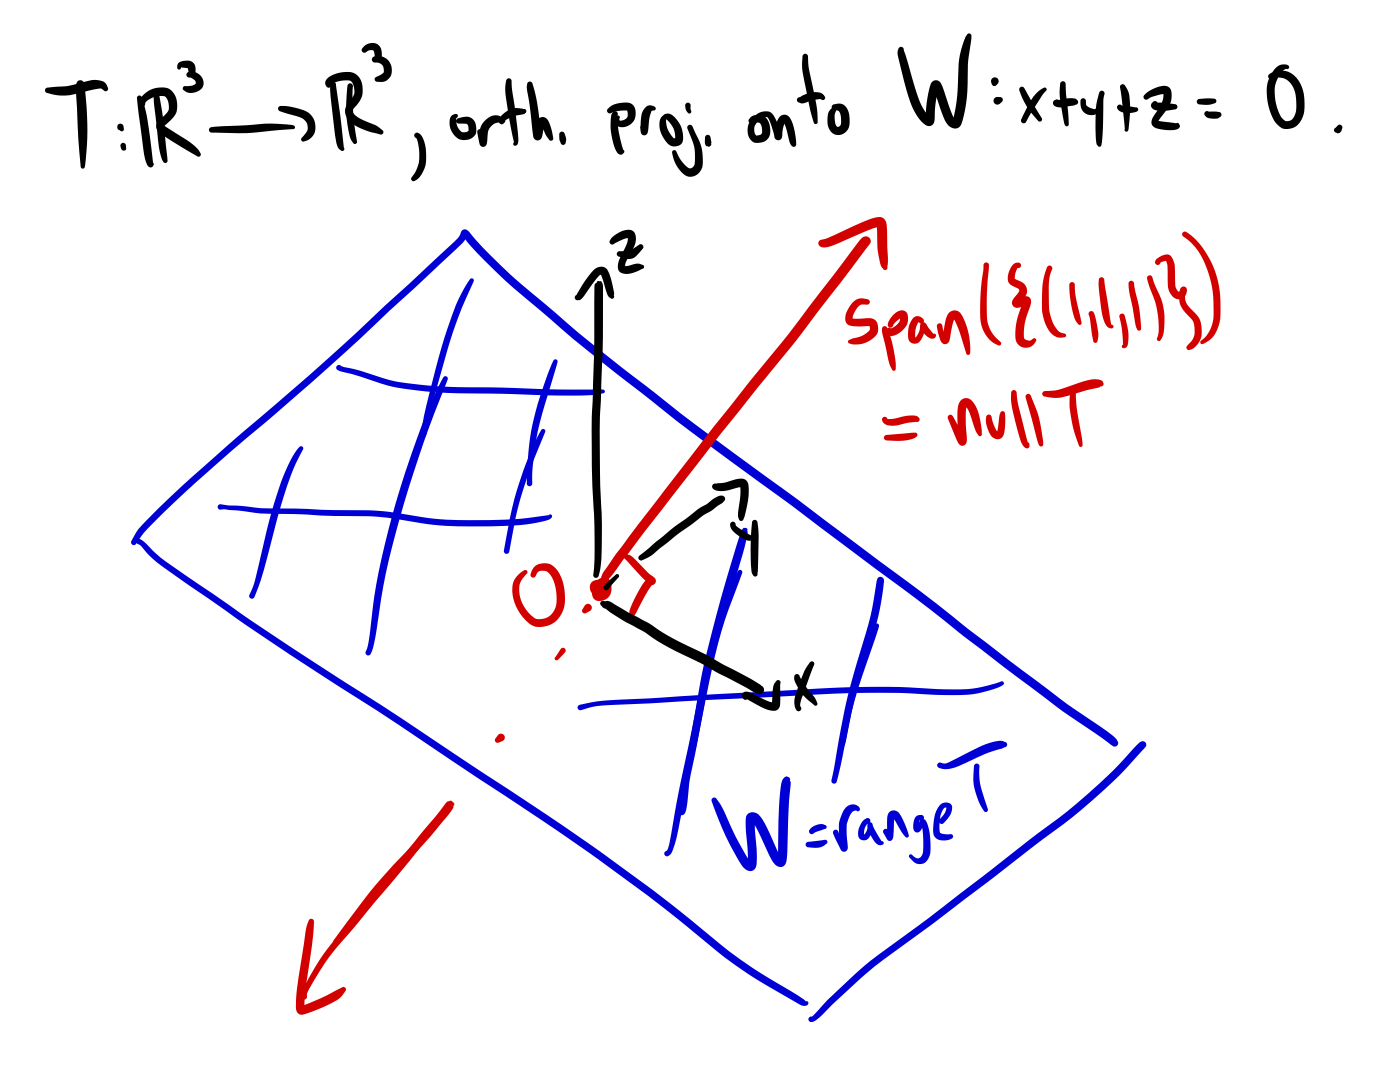
\includegraphics[width=2.5in]{Images/OrthoRankNull}
\]
  \end{example}
\end{frame}
\begin{frame}
 \begin{example}
 Define $T\colon M_{nn}\rightarrow M_{nn}$ as $T(A)=A^T-A$. 
 \bspace 
 As we have seen elsewhere, $\NS T=\{A\in M_{nn}\colon A^T=A\}$ and $\range T=\{A\in M_{nn}\colon A^T=-A\}$, the space of symmetric and skew-symmetric matrices, respectively.  
 \bpause 
 As we have also seen, the dimension of the space of symmetric matrices is $\frac{n(n+1)}{2}$, and the dimension of skew-symmetric matrices is $\frac{n(n-1)}{2}$. 
 \bspace
 According to the rank-nullity theorem we must have 
 \begin{align*}
 n^2&=M_{nn}\\
 &=\dim\NS T+\dim\range T\\
 &=\frac{n(n+1)}{2}+\frac{n(n-1)}{2}.
 \end{align*}
 We have thus given a linear algebraic proof of the identity $n^2=\frac{n(n+1)}{2}+\frac{n(n-1)}{2}$. 
 \bpause
 Yes, there is a more straightforward arithmetic proof, but you must admit this one is pretty cool, and it illustrates how results in one area of mathematics (e.g., linear algebra) can sometimes be translated into results in a completely different area (e.g., combinatorics). 
 
 \end{example}
\end{frame}
\begin{frame}{Relative sizes of $\NS T$ and $\range T$}
Let $T\colon V\rightarrow W$, where $\dim V=n$. Since 
$
\dim\NS T+\dim\range T=n,
$
we see that the {\color{red} bigger} the null space (dimension-wise), the {\color{blue} smaller} the range, and vice versa. 

Let's see this numerically in action. Assume $T\colon V\rightarrow W$ is linear. 
\bb
\pause\ii Suppose $\dim V=5$ and $\dim W=3$. Prove: $\NS T$ is nontrivial. 
\bpause
If $\NS T=\{\boldzero\}$, then $\dim\range T=5-0=5$; but this is impossible since $\range T\subseteq W$ and $\dim W=3$. Thus $\NS T\ne \{\boldzero\}$; i.e., there is a nonzero $\boldv\in\NS T$. This shows $\NS T$ is nontrivial. 
\pause\ii Suppose $\dim V=7$, $\dim W=5$, and $\dim\NS T=2$. Prove: $\range T= W$. 
\bpause 
We have $\dim\range T=7-\dim\NS T=7-2=5$. Since $\range T\subseteq W$ and $\dim\range T=\dim W$, we conclude $\range T=W$. 
\ee
\end{frame}

\begin{frame}{Fundamental subspaces of a matrix}
When $T=T_A$ for some $m\times n$ matrix $A$, we can develop a systematic way of computing bases for $\NS A$ and $\range A$. Not surprisingly this procedure involves Gaussian elimination, as we will outline below. 
\bspace 
In fact the procedure allows us to compute bases for the three following subspaces associated to a matrix, the so-called \alert{fundamental subspaces} of $A$. 

\pause
\begin{definition}
Let $A$ be a an $m\times n$ matrix with rows $\boldr_1,\dots, \boldr_m$ and columns $\boldc_1,\dots \boldc_n$. The following subspaces are called the {\bf fundamental subspaces of $A$}. 
\bb
\ii The {\bf null space} of $A$ is defined as 
\[
\NS A =\{\boldx\in\R^n\colon A\boldx=\boldzero\}\subset \R^n.
\]
\ii The {\bf row space} of $A$ is defined as 
\[
\RS A =\Span(\{\boldr_1,\dots, \boldr_m\})\subset\R^n.
\]
\ii The {\bf column space} of $A$ is defined as 
\[
\CS A=\Span(\{\boldc_1,\dots \boldc_n\})\subset\R^m. 
\]
\ee
\end{definition}
\pause 
The careful reader will object that $\range A$ does not appear on this list! Fear not, as we show in the next slide \alert{$\CS A=\range A$}. 
\end{frame}

\begin{frame}{$\CS A=\range A$}
Take an $m\times n$ matrix and consider $A$ as a collection of $n$ columns $\boldc_j$, each of which lives in $\R^m$:
\[
A=\begin{bmatrix}
\vert&\vert& \cdots &\vert\\
\boldc_1&\boldc_2&\cdots &\boldc_n\\
\vert&\vert& \cdots &\vert
\end{bmatrix}
\]
\pause
Then we have 
\begin{eqnarray*}
\boldb\in\CS A &\Leftrightarrow& \boldb\in\Span(\{\boldc_1,\dots,\boldc_n\})\\
\pause&\Leftrightarrow & \boldb=a_1\boldc_1+a_2\boldc_2+\cdots + a_n\boldc_n \text{ for some $a_i$}\\
\pause&\Leftrightarrow & \boldb=A\begin{bmatrix}
a_1\\ a_2\\ \vdots \\ a_n
\end{bmatrix} \text{ (by column expansion!!)} \\
\pause&\Leftrightarrow & \text{ there is an $\boldx\in\R^n$ such that } A\boldx=\boldb \\
\pause&\Leftrightarrow &\boldb\in \range A.
\end{eqnarray*}
We conclude:
\[
\boxed{\CS A=\range A}
\]
\end{frame}

\begin{frame}{Computing the fundamental spaces}
\footnotesize
Once again Gaussian elimination is the main tool for computing fundamental spaces: start with $A$, row reduce to $U$, compute the fundamental spaces of $U$. However, there are some subtleties involved. Here is the overall description for how to proceed:
\[
\pause 
\begin{array}{lcl}
\text{Space}&\text{Relation}&\text{How to pick a basis}\\
\hline
\text{Null space}&\NS A=\NS U&\left(\begin{array}{c}\text{find vector parametrization}\\ \text{of solutions to $U\boldx=\boldzero$} \end{array}\right) \\
\\
\pause\text{Row space}&\RS A=\RS U &\left(\begin{array}{c}\text{nonzero rows of $U$ }\\ \text{form a basis of $\RS(A)$} \end{array}\right) \\
\\
\pause\text{Column space}&\CS A \alert{\ne}\CS U &\left(\begin{array}{c}\text{pick columns of $A$ corresponding}\\ \text{to columns of $U$ with leading 1's} \end{array}\right) 
\end{array}
\]
\end{frame}
\begin{frame}
Let's prove some of the previous claims. We will begin by proving the following more general result.
\bspace
\alert{Claim}. If $A$ and $B$ are \alert{row equivalent}, then $\NS(A)=\NS(B)$, $\RS(A)=\RS(B)$, and if a certain subset of the columns of $B$ form a basis of $\CS(B)$, then the same is true of the corresponding columns of $A$ and $\CS(A)$. 
\pause
\begin{proof}
First observe that $A$ is row equivalent to $B$ iff $(E_rE_{r-1}\cdots E_1)A=B$ for some elementary matrices $E_i$ iff $QA=B$ for some invertible $Q$. (The latter ``iff" follows since the $E_i$ are elementary, and since all invertible matrices are products of elementary matrices. )
\pause
So we assume $QA=B$ for some invertible $Q$. 
\bpause 
\alert{Null space}. We have shown in an exercise that $A\boldx=\boldzero$ iff $QA\boldx=\boldzero$ iff $B\boldx=\boldzero$. It follows that $\NS(A)=\NS(B)$. 
\bpause
\alert{Row space}
To show $\RS(A)=\RS(B)$, it is enough to show that $\RS(B)\subseteq \RS(A)$; this is because we can then apply the same reasoning using the fact that $A=Q^{-1}B$, $Q^{-1}$ invertible. \pause The row method tells us that each row of $B=QA$ is a linear combination of the rows of $A$. Thus each row of $B$ lies in $\RS(A)$, the span of the rows of $A$. \pause But then we must have $\RS(B)\subseteq\RS(A)$, since $\RS(B)$ is the ``smallest" subspace containing all rows of $B$ (by properties of span).
\bpause
\alert{Column space} (Sketch). Here one can show that columns $\boldc_{i_1}, \boldc_{i_2},\dots, \boldc_{i_r}$ of $A$ form a basis of $\CS(A)$ iff $Q\boldc_{i_1}, Q\boldc_{i_2},\dots, Q\boldc_{i_r}$ form a basis of $\CS(B)$. By the column method the vectors $Q\boldc_{i_j}$ are precisely the corresponding columns of $B=QA$. 
\end{proof}

\end{frame}
\begin{frame}{Example}
\footnotesize
Let's compute bases/dimensions for the fundamental spaces of \\ 
$A=\begin{bmatrix}[rrrr]
2&2&4&2\\
6&6&11&5\\
-4&-4&-7&-3
\end{bmatrix}
$.\\
\pause $A$ reduces to the matrix 
$U=\begin{bmatrix}[rrrr]
1&1&2&1\\
0&0&1&1\\
0&0&0&0
\end{bmatrix}
$
\bpause
First compute 
\[
\NS(U)=\{(s-r,r,-s,s)\colon r, s\in\R\}=\{s(1,0,-1,1)+r(-1,1,0,0)\colon r,s\in\R\}.
\]
It follows that $\NS A=\NS U=\Span \{(1,0,-1,1), (-1,1,0,0)\}$, and thus that $B=\{(-1,1,0,0), (1,0,-1,1)\}$ is a basis for $\NS(A)$. We conclude $\dim\NS A=2$. 
\bpause Next, the rank-nullity theorem implies $\dim\range U=\dim \R^4-\dim\NS U=2$. Thus to choose a basis for $\CS U=\range U$ we need only pick two linearly independent columns of $U$:  the first and third columns will do. It follows that the first and third columns of $A$ form a basis for $\CS A$. This gives us $B''=\{(2,6,-4), (4,11,-7)\}$ as a basis for $\CS A $. 
\bpause
Finally, we have $\RS A =\RS U$, and clearly we can take the nonzero rows of $U$ as a basis for this. Thus $B'=\{(1,1,2,1),(0,0,1,1)\}$ is a basis for $\RS A $. We conclude $\dim\RS A=2$. 
\end{frame}
\begin{frame}
 The preceding example nicely illustrates our general procedure for computing bases for the fundamental spaces of $A$. 
 \begin{block}{Computing bases for the fundamental spaces}
\bb[(i)]
\ii Reduce $A$ to row echelon form matrix $U$. 
\ii $\boxed{\NS(A)=\NS(U)}$. Use free/leading variable method to give full description of solutions $U\boldx=\boldzero$. Extract a basis from the resulting parametric description. 
\ii $\boxed{\RS(A)=\RS(U)}$. A basis for $\RS(U)$ (and hence $\RS(A)$) consists of the nonzero rows of $U$. 
\ii $\boxed{\CS(A)\ne \CS(U)}$. The columns of $U$ with leading 1's are a basis for $\CS(U)$. The {\em corresponding columns} of $A$ form a basis for $\CS(A)$. 
\ee
\end{block}
\pause
\begin{comment}
It is clear that the nonzero rows of $U$ form a basis of $\RS U$: the staircase pattern of leading 1's guarantees they are linearly independent, and we can obviously discard the zero rows. 
\bpause
It is not difficult to show that the columns of $U$ with leading 1's are linearly independent. (Exercise!) That they are in fact a basis follows from the fact that $\#\text{(leading 1's)}=n-\#\text{(free variables)}=n-\dim\NS U=\dim\CS U$. 
\end{comment}
\end{frame}
\begin{frame}{Rank-nullity theorem for matrices}
The previous discussion gives us a much more detailed analysis of the spaces involved in the rank-nullity theorem in the special case where $T=T_A$. We collect some of those details here. 
\begin{block}{Rank-nullity theorem for matrices}
Let $A$ be $m\times n$. Suppose $A$ is row equivalent to the row echelon matrix $U$. 
\bb
\ii $\CS A=\range A$
\ii $\dim\NS A=\#(\text{free variables in the system $U\boldx=\boldzero$})$
\ii $\rank A=\dim\CS A=\dim\RS A=\#(\text{leading 1's in $U$})$
\ii $\rank A\leq \min\{m,n\}$. (Since $\#(\text{leading 1's in $U$})\leq m$ and $\#(\text{leading 1's in $U$})\leq n$.) 
\ii $n=\dim\NS A+\dim\CS A=\dim\NS A+\dim\RS A$. 
\ee
\end{block}
\end{frame}
\begin{frame}{Extending/contracting sets to bases}
Recall that if $\dim V=n$, then any linearly independent set can be \alert{extended} to a basis of $B$, and any spanning set can be \alert{contracted} to a basis. 

In the special case when $V=\R^n$, our fundamental space algorithms provide a means of performing these extensions/contractions. \bpause
Let $\boldv_1,\boldv_2, \dots, \boldv_r\in \R^n$. 
\bb
\ii \alert{Extending to basis}. If the $\boldv_i$ are independent, then to extend to a basis of $\R^n$ proceed as follows:
\bb
\ii Build the matrix $A$ whose columns (in order) are $\boldv_1,\boldv_2, \dots, \boldv_r, \bolde_1,\bolde_2,\dots, \bolde_n$.
\ii Apply the column space algorithm to $A$. 
\ee
\ii \alert{Contracting to basis}. If the $\boldv_i$ span the subspace$W\subseteq\R^n$, then to contract to a basis of $W$ proceed as follows:
\bb
\ii Build the matrix $A$ whose columns are $\boldv_1, \boldv_2, \dots, \boldv_r$. 
\ii Apply the column space algorithm to $A$. 
\ee


\ee
\end{frame}
\begin{frame}{Example}
\footnotesize
Let $W=\Span\{\boldv_1,\boldv_2, \boldv_3, \boldv_4, \boldv_5\}$ where 
\[
\begin{array}{ll}
\boldv_1=(1,-1,5,2)&\boldv_2=(-2,3,1,0)\\
\boldv_3=(4,-5,9,4)&\boldv_4=(0,4,2,-3)\\
\boldv_5=(-7,18,2,-8)
\end{array}
\]
Find a subset of the $\boldv_i$ that yields a basis of $W$. 
\bpause 
We know the $\boldv_i$ span $W$, so to get a basis we need to ``throw out the redundant ones". To figure out which ones need to go, we create a matrix $A$ by setting the $\boldv_i$ as  its \alert{columns} (not its rows)! The procedure for finding a basis for $\CS(A)$ then gives us a subset of these columns that forms a basis.
\bpause 
$A=\begin{bmatrix}[rrrrr]
1&-2&4&0&-7\\
-1&3&-5&4&18\\
5&1&9&2&2\\ 
2&0&4&-3&-8
\end{bmatrix}
\xrightarrow[]{\text{row red.}}
U=
\begin{bmatrix}[rrrrr]
\boxed{1}&0&2&0&-1\\
0&\boxed{1}&-1&0&3\\
0&0&0&\boxed{1}&2\\
0&0&0&0&0
\end{bmatrix}
$
\bpause
It follows that $\{\boldv_1,\boldv_2, \boldv_4\}$ is a basis for $W$. 
\end{frame}
\begin{frame}{Example}
Extend the set $S=\{ (1,1,1,1), (-2,-2,3,3)\}$ to a basis of $\R^4$. 
\bpause
Take the matrix 
\[
A=\begin{bmatrix}
1&-2&1&0&0&0\\
1&-2&0&1&0&0\\
1&3&0&0&1&0\\
1&3&0&0&0&1
\end{bmatrix}
\]
This matrix row reduces to 
\[
U=\begin{bmatrix}
\boxed{1}&-2&1&0&0&0\\
0&\boxed{1}&-1/5&0&1/5&0\\
0&0&\boxed{1}&-1&0&0\\
0&0&0&0&\boxed{1}&-1
\end{bmatrix}
\]
\pause
It follows that the first, second, third and fifth column of $A$ form a basis of $\CS(A)=\R^4$. Thus 
\[
B=\{(1,1,1,1), (-2,-2,3,3), (1,0,0,0), (0,0,1,0)\}
\]
is a basis of $\R^4$ extending $S$. 

\end{frame}
%\begin{frame}{Working in other spaces $V$}
%These algorithms gives us means of computing bases for subspaces inside $\R^n$. What about more exotic vector spaces, like $P_n$, $M_{mn}$, etc.? 
%\bspace 
%The trick when working in one of these more abstract spaces is to first pick a basis $B$ of $V$ (oftentimes the ``standard" one), and use the coordinate vector operator 
%\[
%\boldv\mapsto [\boldv]_B\in\R^n
%\]
%to translate the problem into a question about vectors in $\R^n$. 
%\bpause Use one of the previous algorithms to solve the corresponding problem in $\R^n$, then translate your results back in terms of the original vector space $V$. 
%\bspace The following examples illustrate this technique. 
%\end{frame}
%\begin{frame}{Example}
%Let $W=\Span\{p_1,p_2, p_3, p_4, p_5\}\subset P_3$ where 
%\[
%\begin{array}{ll}
%p_1=1-x+5x^2+2x^3&p_2=-2+3x+x^2\\
%p_3=4-5x+9x^2+4x^3&p_4=4x+2x^2-3x^3\\
%p_5=-7+18x+2x^2-8x^3
%\end{array}
%\]
%Find a subset of the $p_i$ that yields a basis of $W$. 
%\bpause 
%Let $B=\{1,x,x^2, x^3\}$ be the standard basis for $P_3$. Apply $[\hspace{10pt}]_B$ to each of the $p_i$ to get the exact same vectors $\boldv_i$ from the previous example.
%\bpause As we saw in that example, our column space algorithm showed that $\boldv_1, \boldv_2$ and $\boldv_4$ formed a basis for the span of the $\boldv_i$. 
%\bpause 
%It follows that $\{p_1, p_2, p_4\}$ is a basis for $W$ inside $P_3$.
% 
%\end{frame}
%\begin{frame}{Example}
%Let $A_1=\begin{bmatrix}[rr]
%1&1\\-2&0
%\end{bmatrix}
%$,
%$A_2=\begin{bmatrix}[rr]
%1&-1\\-1&1
%\end{bmatrix}
%$,
%$A_3=\begin{bmatrix}[rr]
%1&1\\1&-3
%\end{bmatrix}
%$, and let $W=\Span(\{A_1,A_2,A_3\})$. 
%
%Decide whether $A=\begin{bmatrix}
%1&0\\-1&0
%\end{bmatrix}
%$
%is in $W$. 
%\bpause
%Let $B$ be the standard basis of $M_{22}$. Translate everything to $\R^4$ using $(\underline{\hspace{.2cm}})_B$. 
%\bspace We are then asking whether $\boldv=(1,0,1,0)$ is in the span of $\boldv_1=(1,1,-2,0)$, $\boldv_2=(1,-1,-1,1)$, $\boldv_3=(1,1,1,-3)$. This is equivalent to whether the matrix equation 
%\[
%\begin{bmatrix}[rrr]
%1&1&1\\
%1&-1&1\\
%-2&-1&1\\
%0&1&-3
%\end{bmatrix}
%\boldx
%=\begin{bmatrix}[r]
%1\\ 0\\-1 \\0 
%\end{bmatrix}
%\] 
%has a solution. 
%
%GE shows that in fact we can solve this. (Do it!) This means $\boldv$ is a linear combination of the $\boldv_i$, and thus that $A$ is a linear combination of the $A_i$. 
%
%We conclude $A\in W$. 
%\end{frame}


%\begin{corollary}[Corollary of R-N]
%Let $A$ be $m\times n$. 
%\bb[(i)]
%\pause\ii If $m>n$, then there is a $\boldb\in\R^m$ such that $A\boldx=\boldb$ has no solution (i.e., is inconsistent). 
%\ii If $m<n$, then there is a nontrivial $\boldx\ne\boldzero_n\in\R^n$ such that $A\boldx=\boldzero_m$. 
%\ee
%\pause
%\begin{proof}
%\ \\
%(i) If $m>n$, then $\dim(\CS(A))=\dim(\RS(A))\leq n<m$. Thus $\CS(A)\ne\R^m$, which means there is a $\boldb$ such that $A\boldx=\boldb$ has no solution. 
%\bpause
%(ii) If $m<n$, then $\dim(\CS(A))\leq m<n$. By the R-N theorem we have 
%\[
%\dim(\NS(A))=n-\dim(\CS(A))>n-n=0.
%\]
%Thus $\NS(A)$ is a nontrivial space, which means there is a $\boldx\ne\boldzero_n$ with $A\boldx=\boldzero_m$. 
%\end{proof}
%\end{corollary}
%\end{frame}
\begin{frame}{Invertibility Theorem}
\alert{Suppose $A$ is a square $n\times n$ matrix} . Recall that $A$ is invertible if and only if $A\boldx=\boldzero$ has a unique solution. This is equivalent to $\NS(A)=\{\boldzero\}$. Thus we have: 
\[
A \text{ invertible } \Leftrightarrow \NS(A)=\{\boldzero\}\Leftrightarrow \nullity(A)=0.
\]
\pause Similarly, we have $A$ invertible if and only if $A\boldx=\boldb$ has a solution \alert{for all} $\boldb\in\R^n$. As we saw earlier, $\CS(A)=\{\boldb\in\R^n\colon A\boldx=\boldb \text{ has a solution}\}$. Thus we see that 
\[
A \text{ invertible}\Leftrightarrow \CS(A)=\R^n \Leftrightarrow \rank(A)=n \Leftrightarrow \RS(A)=\R^n,
\]
where the last equivalence follows since $\RS(A)\subset\R^n$ and $\dim(\RS(A))=n$. 
\bpause 
Looks like we have quite a few new statements to add to our Invertibility Theorem! 
\end{frame}
\begin{frame}
\begin{theorem}[Invertibility theorem]
Let $A$ be $n\times n$. The following statements are equivalent. 
\bb[(a)]
\ii $A$ is invertible.
\ii $A\boldx=\boldzero$ has a unique solution (the trivial one). 
\ii $A$ is row equivalent to $I_n$, the $n\times n$ identity matrix.
\ii $A$ is a product of elementary matrices. 	
\ii $A\boldx=\boldb$ has a solution for every $n\times 1$ column vector $\boldb$. 
\ii $A\boldx=\boldb$ has a {\em unique} solution for every $n\times 1$ column vector $\boldb$. 
\ii $\det A\ne 0$.
\ii $\NS A=\{\boldzero\}$.
\ii $\nullity A=0$.
\ii $\rank A=n$. 
\ii $\CS A=\R^n$.
\ii $\RS A=\R^n$.
\ii The columns of $A$ are linearly independent (or span $\R^n$, or are a basis of $\R^n$).
\ii The rows of $A$ are linearly independent (or span $\R^n$, or are a basis of $\R^n$). 
\ee
\end{theorem}

\end{frame}







\subsection{Coordinate vectors}\label{ss:coordinate}
%\begin{frame}<beamer>
%             \frametitle{Outline}
%             \tableofcontents[currentsection,currentsubsection]
%\end{frame}
\begin{frame}{Coordinate vectors relative to a basis $B$}
\begin{definition}
Let $B=\{\boldv_1,\dots ,\boldv_n\}$ be a basis for $V$, and let $\boldv\in V$. According to Theorem \ref{th:basisunique} there is a unique choice of $c_i$ such that 
\[
\boldv=c_1\boldv_1+c_2\boldv_2\cdots +c_n\boldv_n.
\]
We define the {\bf coordinate vector of $\boldv$ relative to the basis $B$} to be the $n$-tuple 
\[
[\boldv]_B:=(c_1,c_2,\dots, c_n)
\]
\end{definition}
\pause
\begin{comments}
\bb
\ii To compute the coordinate vector of $\boldv$ relative to $B=\{\boldv_1,\boldv_2,\dots, \boldv_n\}$ we must \alert{solve} the vector equation $\boldv=c_1\boldv_1+c_2\boldv_2+\cdots +c_n\boldv_n$ for the coefficients $c_1, c_2,\dots, c_n$. 

For any given example this computation can usually be reduced to setting up and solving a certain system of linear equations. 
\pause
\ii As usual, we will be flexible in terms of how we treat the $n$-vector $(c_1,c_2,\dots, c_n)$. For example, we will often interpret this as a $n\times 1$ column vector.  
\ee
\end{comments} 
\end{frame}
\begin{frame}{Example} 
Let $V=P_2$. 
\bb
\ii Let $B=\{1,x, x^2\}$ be the standard basis of $V$. Computing $[p(x)]_B$ in this case is easy since any polynomial $p(x)=a+bx+cx^2$ is already expressed as a linear combination of the elements of $B$ !! 

That is, we have $[a+bx+cx^2]_B=(a,b,c)$ for any polynomial $p(x)=a+bx+cx^2$. 

\pause Some explicit examples:
\begin{align*}
 [7-\pi x+\sqrt{2}x^2]_B&= (7, -\pi, \sqrt{2})\\
 [1+9x^2]_B&=(1,0,9)
\end{align*}
\pause
\ii Let $B'=\{1+x+x^2, -x+x^2, -1+x^2\}=\{p_1,p_2,p_3\}$ be the nonstandard basis we considered earlier. Now it requires more work to compute $[p(x)]_{B'}$. 
\pause Some explicit examples:
\begin{eqnarray*}
1+x+x^2=1p_1+0p_2+0p_3&\Rightarrow&[1+x+x^2]_{B'}=(1,0,0)\\
-x+x^2=0p_1+1p_2+0p_3&\Rightarrow&[-x+x^2]_{B'}=(0,1,0)\\
x^2=\frac{1}{3}p_1+\frac{1}{3}p_2+\frac{1}{3}p_3&\Rightarrow& [x^2]_{B'}=(\frac{1}{3},\frac{1}{3},\frac{1}{3})
\end{eqnarray*}
\ee
\pause The last example was computed by setting up the polynomial equation $x^2=c_1(1+x+x^2)+c_2(-x+x^2)+c_3(-1+x^2)$ and solving for the $c_i$. Verify for yourself that $c_1=c_2=c_3=1/3$ is the solution!

\end{frame}

\begin{frame}{Coordinate vector map}
\begin{theorem}\label{th:coordinates}
Let $V$ be a vector space, and suppose $B=\{\boldv_1,\boldv_2,\dots, \boldv_n\}$ be a basis for $V$. Define 
\begin{align*}
T\colon V&\rightarrow \R^n\\
\boldv&\mapsto [\boldv]_B.
\end{align*}
\bb
\ii  $T$ is a linear transformation. We will call $T$ the {\bf coordinate vector map with respect to $B$}.

\ii $T(\boldv_1)=T(\boldv_2)$ if and only if $\boldv_1=\boldv_2$: i.e., $T$ is \alert{one-to-one}. 

In particular, $T(\boldv)=\boldzero$ if and only if $\boldv=\boldzero_V$. 

\ii  $\range T=\R^n$: i.e. $T$ is \alert{onto}. 

\ii  A set $S=\{w_1,w_2,\dots, w_r\}\subseteq V$ is linear independent  if and only if $T(S)=\{T(\boldw_1), T(\boldw_2),\dots, T(\boldw_r)\}\subseteq \R^n$ is linearly independent. 

\ii A set $S=\{w_1,w_2,\dots, w_r\}\subseteq V$ spans $V$ if and only if $T(S)=\{T(\boldw_1), T(\boldw_2),\dots, T(\boldw_r)\}$ spans $\R^n$. 
\ee
\end{theorem}
 \begin{proof}
 Exercise.
 \end{proof}
\end{frame}
\begin{frame}
Fix vector space $V$ and basis $B=\{\boldv_1,\boldv_2,\dots, \boldv_n\}$. According to Theorem \ref{th:coordinates}, the coordinate vector map $\boldv\mapsto [\boldv]_B$ is not only \alert{linear}, it is also \alert{1-1 and onto}.  Such functions are called \alert{isomorphisms}.  
\pause
\begin{definition}
Let $V$ and $W$ be vector spaces. An {\bf isomorphism} is a linear transformation $T\colon V\rightarrow W$ that is 1-1 and onto. 

The spaces $V$ and $W$ are called {\bf isomorphic} in this case. 
\end{definition}
\pause
\begin{comment}
`Isomorphism' is derived from the Greek terms `isos', meaning ``equal", and `morphe', meaning ``form". 
\bspace
We do not have time in the course to study isomorphisms in detail. Instead we content ourselves with the following \alert{general principle}:  when $V$ and $W$ are isomorphic, as witnessed by an isomorphism $T\colon V\rightarrow W$, the spaces are identical as far as vector space structure is concerned, even though as sets they may look completely different. 
\bpause
Furthermore, since $T$ is 1-1 and onto, it has an inverse function $T^{-1}\colon W\rightarrow V$. Furthermore, you can show that $T^{-1}$ is also a linear transformation. The two functions $T$ and $T^{-1}$ allow us to to go back and forth between $V$ and $W$, translating statements about $V$ into corresponding statements about $W$ with no information loss. 
\end{comment}
\end{frame}
\begin{frame}
We apply the general principle described in the previous slide to the special case of a coordinate vector isomorphism 
$[\hspace{10pt}]_B\colon V\rightarrow \R^n$. 
 \begin{block}{Coordinate vector technique} Suppose we have chosen a finite basis $B$ for the vector space $V$. 
 Let $[\hspace{10pt}]_B$ denote the corresponding coordinate vector map, and let $[\hspace{10pt}]_B^{-1}$ denote the inverse of this map.
 
 Any linear algebraic questions we want to answer about $V$ (involving span, linear independence, etc.) can be answered as follows: 
\bb
\ii First apply $[\hspace{10pt}]_B$ to all vectors $\boldv$ in question. 
\ii Answer the corresponding question in $\R^n$ about the column vectors $[\boldv]_B$. 
\ii If necessary, translate your results back to the setting of $V$ by applying the inverse $[\hspace{10pt}]_B^{-1}$. 
\ee
\end{block}

\end{frame}
\begin{frame}{Example}
The set 
\[
S=\left \{ A_1=\begin{bmatrix}
2&1\\
0&-2
\end{bmatrix}, A_2=\begin{bmatrix}
1&1\\
1&-1
\end{bmatrix}, 
A_3=\begin{bmatrix}
0&1\\
2&0
\end{bmatrix},
A_4=\begin{bmatrix}
-1&0\\
1&1
\end{bmatrix}\right\}
\]
is a subset of the space $W=\{ A\in M_{22}\colon \tr A=0\}$. (Recall: the trace of a matrix, $\tr A$, is defined as the sum of its diagonal elements. )

Contract $S$ to a basis of $\Span S$, and determine whether $\Span S=W$. Use the coordinate vector map technique! 
\bpause 
We must first pick a basis for $W$. Observe that the general element of of $W$ can be described as 
\[
\begin{bmatrix}a&b\\
c&-a\end{bmatrix}
=a\underset{B_1}{\underbrace{\begin{bmatrix}
1&0\\
0&-1
\end{bmatrix}}}+b\underset{B_2}{\underbrace{\begin{bmatrix}
0&1\\
0&0
\end{bmatrix}}}+c\underset{B_3}{\underbrace{\begin{bmatrix}
0&0\\1&0
\end{bmatrix}}}.\]
It follows easily that $B=\{B_1,B_2, B_3\}$ is a basis for $W$. 
\bpause
Apply $[\hspace{10pt}]_B$ to the elements of the given $S$ to get a corresponding set $S'\subseteq\R^3$:
\[
S'=\left\{ [A_1]_B=(2,1,0), [A_2]_B=(1,1,1), [A_3]_B=(0,1,2), [A_4]_B=(-1,0,1)\right\}
\]
\pause
Now use the ``contract to basis" algorithm on $S'$ to conclude that the set $\{(2,1,0), (1,1,1)\}$ forms a basis for $\Span S'$. Translating back to $W$, we see that $A_1$ and $A_2$ form a basis for $\Span S$, that $\dim\Span S=2$, and hence that $\Span S\ne W$, since $\dim W=3$. 
\end{frame}

\subsection{Matrix representations}\label{ss:matrixreps}
\begin{frame}<beamer>
             \frametitle{Outline}
             \tableofcontents[currentsection,currentsubsection]
\end{frame}
\begin{frame}{Matrix representations of transformations}
We have seen how the coordinate vector map can be used to translate a linear algebraic question posed about the exotic vector space $V$ into a question about the more familiar vector space $\R^n$, where we have many computational algorithms at our disposal. 

We would like to extend this technique to linear transformations $T\colon V\rightarrow W$, where both $V$ and $W$ are \alert{finite-dimensional}. The basic idea, to be fleshed out below, can be described as follows: 
\bb
\ii Pick a basis $B$ for $V$, and a basis $B'$ for $W$. 
\ii ``Identify" $V$ with $\R^n$ and $W$ with $\R^m$ using the coordinate vector isomorphisms $[\hspace{10pt]}_B$ and $[\hspace{10pt}]_{B'}$, respectively. 
\ii ``Model" the linear transformation $T\colon V\rightarrow W$ with a certain linear transformation $T_A\colon \R^n\rightarrow \R^m$.
\ee
\pause The matrix $A$ defining $T_A$ will be called the \alert{matrix representing $T$ with respect to our choice of basis $B$ for $V$ and $B'$ for $W$}. 
\bpause In what sense does $A$ ``model" $T$? All the properties of $T$ we are interested in ($\NS T$, $\nullity T$, $\CS T$, $\rank T$, etc.) are perfectly mirrored by the matrix $A$. 
\bpause 
As a result, this technique allows us to answer questions about the original $T$ essentially by applying a relevant matrix algorithm to $A$.
 
\end{frame}
\begin{frame}{Matrix representations of transformations}
Given: $T\colon V\rightarrow W$ a linear transformation, $\dim V=n$, $\dim W=m$. 
\bspace
First \alert{choose} bases $B=\{\boldv_1,\dots,\boldv_n\}$ for $V$ and $B'=\{\boldw_1,\dots,\boldw_m\}$ for $W$.  These two bases give rise to two coordinate vector isomorphisms: 
\begin{align*}
[\hspace{5pt}]_B\colon V&\rightarrow \R^n\\
[\hspace{5pt}]_{B'}\colon W&\rightarrow \R^m
\end{align*}
\pause Putting all three of these maps together yields the diagram 
\[
\xymatrix@C=2pc @R=2.5pc{
V\ar[r]^{T} \ar@{<->}[d]_{[\hspace{5pt}]_B}& W \ar@{<->}[d]^{[\hspace{5pt}]_{B'}}\\
\R^n & \R^m
}
\]
where the double-headed arrows indicate the fact that the coordinate maps are isomorphisms: i.e., we also have inverse maps $([\hspace{5pt}]_B)^{-1}$, $([\hspace{5pt}]_{B'})^{-1}$ going up.

The \alert{matrix $A$ representing $T$ with respect to the bases $B$ and $B'$} will be the matrix that ``completes" this diagram by supplying an arrow from $\R^n$ to $\R^m$. 

\bpause 
Crucial in our discussion will be the theorem stating that
\bb[(i)]
\ii a linear transformation can be defined simply by declaring where basis elements are sent, and 
\ii the linear transformation is uniquely determined by this choice.
\ee
%\pause
%\alert{From now on coordinate vectors will be treated as column vectors}. As such we adjust the notation a bit: %instead of $(\boldv)_B=(k_1,k_2,\dots,k_n)$, we write 
%\[
%[\boldv]_B=\begin{bmatrix}
%k_1\\ \vdots \\ k_n
%\end{bmatrix}
%\]
\end{frame}
\begin{frame}
\footnotesize
So we want a matrix $A$ ``completing" the previous diagram like so:
\[
\xymatrix@C=2pc @R=2.5pc{
V\ar[r]^{T} \ar@{<->}[d]_{[\hspace{5pt}]_B}& W \ar@{<->}[d]^{[\hspace{5pt}]_{B'}}\\
\R^n\ar[r]_{A}& \R^m
}
\] 
\pause
More precisely, we want the diagram to be \alert{commutative}. 
\bspace This means that if we start at $V$ and go right with $T$, then down with $[\hspace{5pt}]_{B'}$, this is the same as first going down with $[\hspace{5pt}]_{B}$, then right with $A$. 
\bpause
In terms of function compositions this means we want $[\hspace{5pt}]_{B'}\circ T=A\circ[\hspace{5pt}]_{B}$, or equivalently 
\[
\boxed{[T(\boldv)]_{B'}=A[\boldv]_B, \text{ for all $\boldv\in V$}}.
\]
\end{frame}
\begin{frame}{Computing the matrix $A$}
\footnotesize
$
\hfill
\boxed{[T(\boldv)]_{B'}=A[\boldv]_B, \text{ for all $\boldv\in V$}}.
\hfill
$
\\
We now use the boxed condition to compute $A$ column by column. Let $\boldc_j$ denote the $j$-th column of $A$. 
\bpause By the column method of matrix multiplication we have 
\begin{eqnarray*}
\boldc_j&=&A\bolde_j \text{ ($\bolde_j$ the $j$-th element of standard basis)}\\
\pause&=&A[\boldv_j]_B \text{ ($\boldv_j$ the $j$-th element of basis $B$)}\\
\pause&=&[T\boldv_j]_{B'}
\end{eqnarray*}
\pause
Thus we have a formula for computing the $j$-th column of $A$:
\[
\boxed{\boldc_j=[T[v_j]]_{B'}}
\]
\pause The matrix $A$ we obtain in this fashion is called the {\bf matrix for $T$ relative to the bases $B$ and $B'$}, and is denoted $A=[T]_{B}^{B'}$. 
\end{frame}
\begin{frame}
Let's record our results as a theorem. 
\begin{theorem}[Matrix representation theorem]
Let $V, W$ be finite-dimensional vector spaces, let $T\colon V\rightarrow W$ be linear, let $B=\{\boldv_1,\boldv_2,\dots, \boldv_n\}$ be a basis for $V$, and let $B'$ be a basis for $W$. There is a \alert{unique} matrix $A$ satisfying the following property: 
\[
[T(\boldv)]_{B'}=A[\boldv]_B \text{ for all $\boldv\in V$}.
\]
The matrix is denoted $A=[T]_B^{B'}$ and can be computed column by column using the recipe $\bolda_j=[T(\boldv_j)]_{B'}$, where $\bolda_j$ is the $j$-th column of $A$. 
\end{theorem}
\pause
The theorem is summed up by the following \alert{commutative diagram}:
\[
\xymatrix@C=2pc @R=2.5pc{
V\ar[r]^{T} \ar@{<->}[d]_{[\hspace{5pt}]_B}& W \ar@{<->}[d]^{[\hspace{5pt}]_{B'}}\\
\R^n\ar[r]_{A=[T]_B^{B'}}& \R^m
}
\] 
\pause
\begin{corollary}[Computational method]
Any question about the \alert{linear transformation} $T$ can be answered by first answering the analagous question for the \alert{matrix}  $A=[T]_B^{B'}$, and then translating your results back to $V$ and $W$ using $[\hspace{5pt}]_B^{-1}$ and $[\hspace{5pt}]_{B'}^{-1}$. 
\end{corollary}
\end{frame}
\begin{frame}{Example}
Define $T\colon P_{3}\rightarrow P_{2}$ by $T(p(x))=p'(x)$. Compute $A=[T]_{B}^{B'}$, where $B$ and $B'$ are the standard bases for $P_3$ and $P_2$, respectively. 

Use $A$ to determine $\NS T$ and $\range T $. 
\begin{bsolution}
The matrix $A$ will be $3\times 4$. Denote by $\boldc_j$ the $j$-th column of $A$. We use the formula for $\boldc_j$:
\begin{align*}
\boldc_1&=[T(1)]_{B'}=[0]_{B'}=\begin{bmatrix}
0\\ 0 \\ 0
\end{bmatrix} &
\boldc_2&=[T(x)]_{B'}=[1]_{B'}=\begin{bmatrix}
1\\ 0 \\ 0
\end{bmatrix}\\
\boldc_3&=[T(x^2)]_{B'}=[2x]_{B'}=\begin{bmatrix}
0\\ 2 \\ 0 
\end{bmatrix} &
\boldc_4&=[T(x^3)]_{B'}=[3x^2]_{B'}=\begin{bmatrix}
0\\ 0 \\ 3
\end{bmatrix}
\end{align*}
\pause Thus $A=\begin{bmatrix}
0&1&0&0\\ 0&0&2&0\\ 0&0&0&3
\end{bmatrix}$. 

\pause We see easily that $\NS A =\Span(\{(1,0,0,0)\})$ and $\range A=\CS A=\R^3$. Translating everything back to the original spaces, we see that $\NS(T)=\Span(\{1\})=\{\text{constant poly.'s}\}$ and $\range(T)=P_2$. 
\end{bsolution}
\end{frame}
\begin{frame}
In the special case where $T\colon V\rightarrow V$ maps a space $V$ \alert{to itself}, when representing $T$ with a matrix, we usually just pick a single basis $B$ for $V$ and compute 
\[
A=[T]_{B}^{B}=:[T]_B \hspace{5pt} \text{ (our notation drops the redundant $B$)}
\]
\bpause
\alert{Example}. Define $T\colon M_{22}\rightarrow M_{22}$ by $T(A)=A^T+A$. 
\bspace
Let $B$ be the standard basis of $M_{22}$, and let 
\[
B'=\{
\begin{bmatrix}
0&1\\
-1&0
\end{bmatrix},
\begin{bmatrix}
1&0\\
0&0
\end{bmatrix},
\begin{bmatrix}
0&1\\
1&0
\end{bmatrix},
\begin{bmatrix}
0&0\\
0&1
\end{bmatrix}
\}.
\]
\bb
\ii Compute $A=[T]_B$. 
\ii Compute $A'=[T]_{B'}$.
\ee
\begin{bsolution}
\[ A=\begin{bmatrix}
2&0&0&0\\
0&1&1&0\\
0&1&1&0\\
0&0&0&2
\end{bmatrix}, A'=\begin{bmatrix}
0&0&0&0\\
0&2&0&0\\
0&0&2&0\\
0&0&0&2
\end{bmatrix}
\]
\end{bsolution}
\alert{Moral:} our choice of basis affects the matrix representing $T$, and some choices are better than others!
\end{frame}
\begin{frame}{$\R^n$ revisited}
Consider the \alert{special case} of the form $T\colon \R^n\rightarrow \R^m$. We know that in this case we have $T=T_A$, where 
\[
A=
\begin{bmatrix}
\vert&\vert&\cdots &\vert \\
T(\bolde_1)& T(\bolde_2)&\cdots &T(\bolde_n)\\
\vert&\vert&\cdots &\vert
\end{bmatrix}.
\] 
In light of our recent discussion we recognize this as simply $A=[T]_{B}^{B'}$, where $B,B'$ are the \alert{standard bases} of $\R^n$ and $\R^m$. 

\bpause
This is certainly the most direct way of associating a matrix to the transformation $T$ in this case, but it begs the question as to whether another choice of bases gives us a \alert{better} matrix representation!

Example follows. 
\end{frame}
\begin{frame}{Example}
Let $W\colon x+y+z=0$ be the plane in $\R^3$ perpendicular to $\boldn=(1,1,1)$, and consider the orthogonal projection transformation $T=\text{proj}_W\colon \R^3\rightarrow \R^3$. 
\bpause
The recipe in the last slide tells us that $\text{proj}_W=T_A$ where $A=\begin{bmatrix}[rrr]2/3 &-1/3&-1/3\\-1/3&2/3&-1/3\\ -1/3&-1/3&2/3
\end{bmatrix}
$. 
\bpause
This $A$ is nothing more than $[T]_B$, where $B=\{\bolde_1,\bolde_2,\bolde_3\}$ is the \alert{standard basis} of $\R^3$. We ask: Is there another basis $B'$ for which the matrix $A'=[T]_{B'}$ is simpler? 
\bpause
Yes!! I'll build a basis that pays more attention to the geometry involved in defining $T$. Start first with a basis of the plane $W$: the set $\{\boldv_1=(1,-1,0),\boldv_2=(0,1,-1)\}$ will do. Now \alert{extend} to a basis of $\R^3$. We need only add a vector that is not included already in $W$: the normal vector $\boldv_3=(1,1,1)$ to the plane is a natural choice. 

\pause Thus we consider the basis $B'=\{\boldv_1,\boldv_2, \boldv_3\}$ and compute $A'=[\text{proj}_W]_{B'}$:
{\scriptsize
$
A'=\begin{bmatrix}
\vert&\vert&\vert\\
[T(\boldv_1)]_{B'}&[T(\boldv_2)]_{B'}&[T(\boldv_3)]_{B'}\\
\vert&\vert&\vert
\end{bmatrix}
\pause=
\begin{bmatrix}[ccc]
\vert&\vert&\vert\\
[\boldv_1]_{B'}&[\boldv_2]_{B'}&[\boldzero]_{B'}\\
\vert&\vert&\vert
\end{bmatrix}
\pause =\begin{bmatrix}
1&0&0\\
0&1&0\\
0&0&0
\end{bmatrix}
$
}
\bpause Wow, $A'$ is way simpler! How can both of these matrices ``represent" the same linear transformation?
\end{frame}
\begin{frame}\frametitle{Example continued} 

{\scriptsize Let $W\colon x+y+z=0$ be a the plane in $\R^3$ perpendicular to $\boldn=(1,1,1)$, and consider the orthogonal projection transformation $T=\text{proj}_W\colon \R^3\rightarrow \R^3$. 

Two different bases: 
$B=\{\bolde_1,\bolde_2,\bolde_3\}$,$B'=\{\boldv_1=(1,-1,0),\boldv_2=(0,1,-1), \boldv_3=(1,1,1)\}$.

Two different matrix representations: 

$A=[T]_B=\frac{1}{3}\begin{bmatrix}[rrr]2 &-1&-1\\-1&2&-1\\ -1&-1&2
\end{bmatrix}$, 
$A'=[T]_{B'}=\begin{bmatrix}
1&0&0\\
0&1&0\\
0&0&0
\end{bmatrix}$.}
\bpause
The simpler matrix $A'$ gives us a clear \alert{conceptual} understanding of this orthogonal projection. 

\pause For example, we see that $\CS A'=\Span(\{(1,0,0),(0,1,0)\})$ and $\NS A'=\Span(\{(0,0,1)\}$, and furthermore $A'$ acts as the identity on $\CS A'$, and as the zero transformation on $\NS A'$. 
\bpause Using $[\hspace{5pt}]_{B'}^{-1}$ we can translate this information back to $T=\text{proj}_W$. Namely, $\range T=\Span\{(\boldv_1,\boldv_2)\}=W$, $\NS T=\Span \{\boldv_3\}=\Span \{\boldn\}$, and furthermore, $T$ acts as the identity on $W$ and as the zero transformation on $\Span\{\boldn\}$.  
\bpause
However, if we actually want an \alert{explicit formula} for computing he orthogonal projection of a vector $\boldx\in \R^3$ onto $W$, we are better off using $A$, since we have $\proj{\boldx}{W}=A\boldx$.  
\bpause
So both representations have their own particular virtue! In the next section we develop a means for fluidly going back and forth between the two.
\end{frame}
%\begin{frame}{Example concluded}
%For example to compute $T(\boldx)$ with $\boldx=(1,2,1)$ using $A'$ we must first represent $\boldx$ in terms of $B'$: 
%\begin{align*}
%\boldx&=-\frac{1}{3}\boldv_1+\frac{1}{3}\boldv_2+\frac{4}{3}\boldv_3 &\text{(not obvious; I used GE)}\\
%&\Rightarrow [\boldx]_B'=\frac{1}{3}\begin{bmatrix}[r]
%-1\\ 1\\4 
%\end{bmatrix}.
%\end{align*}
%\pause
%Next, using the defining property, we compute 
%\[
%[T(\boldx)]_{B'}=
%A'[\boldx]_{B'}=\begin{bmatrix}
%1&0&0\\
%0&1&0\\
%0&0&0
%\end{bmatrix}
%\left(\frac{1}{3}\begin{bmatrix}[r]
%-1\\ 1\\4 
%\end{bmatrix}\right)=
%\frac{1}{3}\begin{bmatrix}[r]
%-1\\ 1\\0
%\end{bmatrix}
%\]
%\pause
%Lastly, since $[T(\boldx)]_{B'}=\frac{1}{3}(-1,1,0)$, we conclude that $T(\boldx)=-\frac{1}{3}\boldv_1+\frac{1}{3}\boldv_2+0\boldv_3=\frac{1}{3}(-1,2,-1)$.
%
%\bpause Wouldn't it have been easier just to compute 
%\[
%A\begin{bmatrix}
%1\\2 \\1
%\end{bmatrix}
%=\frac{1}{3}\begin{bmatrix}[rrr]2 &-1&-1\\-1&2&-1\\ -1&-1&2
%\end{bmatrix}\begin{bmatrix}
%1\\2 \\1
%\end{bmatrix}=\frac{1}{3}
%\begin{bmatrix}[r]
%-1\\2\\-1
%\end{bmatrix}
%?
%\] 
%\end{frame}

\subsection{Change of basis}
\begin{frame}<beamer>
             \frametitle{Outline}
             \begin{multicols}{2}
             \tableofcontents[currentsection,currentsubsection]
             \end{multicols}{2}
\end{frame}
\begin{frame}{Change of basis}
We have seen how the coordinate vector map $[\hspace{10pt}]_B$ and matrix representations $[T]_B^{B'}$ are two invaluable computational tools for dealing with abstract vector spaces. 
\bpause 
As the notation indicates, both of these operations depend essentially on your \alert{choice of basis or bases}.
This gives rise to the following questions: 
\bb
\ii Given $V$ and two choices of basis, $B$ and $B'$, what is the relation between $[\boldv]_B$ and $[\boldv]_{B'}$?
\ii GIven $T\colon V\rightarrow W$ and two choices of pairs of bases, $(B, B')$ and $(B'', B''')$, what is the relation between $[T]_{B}^{B'}$ and $[T]_{B''}^{B'''}$?
\ee
\pause 
We will tackle both questions in turn. Both answers rely on something called a \alert{change of basis matrix} $\underset{B\rightarrow B'}{P}$. 
\bpause
For question (2), we will look at the slightly less general situation where $T\colon V\rightarrow V$: i.e., the situation where $W=V$, and we choose the same basis for the domain and codomain. I leave the full general case as an exercise. 
\end{frame}
\begin{frame}{Change of basis matrix}
\begin{block}{Theorem/Definition} Given a vector space $V$ of dimension $n$, and two different bases $B$ and $B'$, there is a \alert{unique} $n\times n$ matrix $\underset{B\rightarrow B'}{P}$ satisfying the following defining property:
\[
\underset{B\rightarrow B'}{P}[\boldv]_B=[\boldv]_{B'}.
\]
The matrix $\underset{B\rightarrow B'}{P}$ is called the {\bf change of basis matrix (or transition matrix) from $B$ to $B'$}. 
\end{block}
\bpause
\begin{proof}[Proof/recipe] Let $B=\{\boldv_1,\dots, \boldv_n\}$ and let $B'=\{\boldw_1,\dots,\boldw_n\}$. 

We build $\underset{B\rightarrow B'}{P}$ \alert{column by column}: specifically, $\underset{B\rightarrow B'}{P}$ is the matrix whose $j$-th column is  
\[
\boxed{\boldp_j=[\boldv_j]_{B'}};
\]
i.e., to compute the $j$-th column of $\underset{B\rightarrow B'}{P}$ you must find the $B'$-coordinates of the $j$-th basis element of $B$.  

\pause Thus defined, one can show using the column method that $\underset{B\rightarrow B'}{P}[\boldv_j]_{B}=[\boldv_j]_{B'}$. One then argues that if the condition is true for each basis element $\boldv_j$, then it must be true for all $\boldv$. (Ask your professor for details!) 
\end{proof}
\end{frame}
\begin{frame}
\alert{Example}. For any vector space $V$ and basis $B$, we have $\underset{B\rightarrow B}{P}=I$. 
\bpause
Indeed for any vector $\boldv$, we have $I[\boldv]_B=[\boldv]_B$. Thus $I$ satisfies the defining property of $\underset{B\rightarrow B}{P}$. By uniqueness, it follows that $I=\underset{B\rightarrow B}{P}$ !!
\bpause
\alert{Example}. Let $V=\R^2$. Compute $\underset{B\rightarrow B'}{P}$ where $B=\{\boldv_1=(1,1),\boldv_2=(1,-1)\}$ and $B'=\{(1,2),(2,1)\}$. 

Test that the matrix converts correctly using the vector $\boldv=1(1,1)+3(1,-1)=(4,-2)$. 
\begin{bsolution}
The recipe tells us that 
\begin{eqnarray*}
\underset{B\rightarrow B'}{P}&=&\begin{bmatrix}
\vert &\vert \\
\hspace{7pt}[\boldv_1]_{B'} &\hspace{7pt}[\boldv_2]_{B'}\\
\vert &\vert 
\end{bmatrix}\\
\pause&=&\begin{bmatrix}[rr]1/3&-1\\
1/3&1
\end{bmatrix} \hspace{8pt}\text{(after some computation)}
\end{eqnarray*}
\pause For $\boldv=1(1,1)+3(1,-1)=(4,-2)$, we have $(\boldv)_B=(1,3)$. Thus we should have 
\[
[\boldv]_{B'}=\underset{B\rightarrow B'}{P}[\boldv]_B=\begin{bmatrix}[rr]1/3&-1\\
1/3&1
\end{bmatrix}\begin{bmatrix}
1\\ 3
\end{bmatrix}=\begin{bmatrix}
-8/3\\
10/3 
\end{bmatrix}.
\]
\pause Indeed, one easily verifies that $(4,-2)=-8/3(1,2)+10/3(2,1)$. 
\end{bsolution}

\end{frame}
\begin{frame}{Example}
Take $V=P_2$, $B=\{1,x,x^2\}$ and $B'=\{1,(x-2), (x-2)^2\}$. Compute $\underset{B\rightarrow B'}{P}$. 
\bpause
Follow the recipe: let $\boldp_j$ be the $j$-th column of $\underset{B\rightarrow B'}{P}$. We have (after some computation)
\[
\boldp_1=[1]_{B'}=(1,0,0), \ \boldp_2=[x]_{B'}=(2,1,0), \ \boldp_3=[x^2]_{B'}=(4,4,1).
\]
Thus $\underset{B\rightarrow B'}{P}=\begin{bmatrix}1&2&4\\ 0&1&4\\ 0&0&1  \end{bmatrix}$
\bpause
Let's check with the test vector $p(x)=1+x+x^2$. We have $(p)_B=(1,1,1)$. Thus we should have 
$
[p]_{B'}=\underset{B\rightarrow B'}{P}[p]_B=\begin{bmatrix}1&2&4\\ 0&1&4\\ 0&0&1  \end{bmatrix}\begin{bmatrix}1 \\ 1 \\ 1\end{bmatrix}=\begin{bmatrix}
7\\ 5\\ 1
\end{bmatrix}$.
Equivalently, this means that $p(x)=7+5(x-2)+(x-2)^2$, as one easily verifies. 

\framebreak
\pause\alert{Cool fact}. We could have derived the last equality using the theory of Taylor series. Namely any polynomial can be ``expanded around $x=a$" as 
$
p(x)=\sum_{i=0}^n\frac{p^{(i)}(a)}{a!}(x-a)^i.
$

More generally, this means 
\[
(p(x))_{B'}=(p(a), p'(a), p''(a)/2, \dots , p^{(n)}(a)/n!)
\]
where $B'=\{1,x-a, (x-a)^2,\dots , (x-a)^n\}$. 
\end{frame}
\begin{frame}
\alert{Theorem}. Let $V$ be a vector space of dimension $n$, and let $B$ and $B'$ be two different bases of $V$. 

The change of basis matrix $\underset{B\rightarrow B'}{P}$ is invertible. In fact we have 
\[
(\underset{B\rightarrow B'}{P})^{-1}=\underset{B'\rightarrow B}{P}
\]
\pause
\alert{Proof}. \scriptsize 
I will show that $\underset{B'\rightarrow B}{P}\cdot\underset{B\rightarrow B'}{P}=I_n$, proving that both matrices are invertible, and are in fact the inverses of one another. My proof will only make use of the defining property of change of basis matrices, and their uniqueness.

For any $\boldv$ we compute:
\begin{eqnarray*}
\underset{B'\rightarrow B}{P}\cdot\underset{B\rightarrow B'}{P}[\boldv]_B&=&\underset{B'\rightarrow B}{P}(\underset{B\rightarrow B'}{P}[\boldv]_B)\\
\pause&=&\underset{B'\rightarrow B}{P}[\boldv]_{B'} \hspace{5pt} \text{(prop. of $\underset{B\rightarrow B'}{P}$)}\\
\pause&=&[\boldv]_{B} \hspace{25pt} \text{(prop. of $\underset{B'\rightarrow B}{P}$)}
\end{eqnarray*}
\pause
Thus $\underset{B'\rightarrow B}{P}\cdot\underset{B\rightarrow B'}{P}[\boldv]_B=[\boldv]_B$ for all $\boldv\in V$. But this means $\underset{B'\rightarrow B}{P}\cdot\underset{B\rightarrow B'}{P}$ satisfies the defining property of $\underset{B\rightarrow B}{P}$.  
\bpause
By \alert{uniqueness} of the change of basis matrix, we must have 
\[
\underset{B'\rightarrow B}{P}\cdot\underset{B\rightarrow B'}{P}=\underset{B\rightarrow B}{P}
\]
\pause Lastly, in a previous example we showed that $P_{B\rightarrow B}=I_n$. Thus, 
\[
\underset{B'\rightarrow B}{P}\cdot\underset{B\rightarrow B'}{P}=\underset{B\rightarrow B}{P}=I_n,
\]
as claimed. 

\end{frame}
\begin{frame}{Example: $V=\R^n$ and $B$ is standard}
Consider the simple example where $V=\R^n$, $B$ is the standard basis, and $B'=\{\boldv_1,\dots,\boldv_n\}$ is some nonstandard basis. 
\bspace
I claim the matrix $P=\begin{bmatrix}\vert&\dots &\vert \\ \boldv_1&\cdots&\boldv_n\\ \vert&\dots &\vert \end{bmatrix}$ whose columns are the elements of $B'$ is the change of basis matrix $\underset{B'\rightarrow B} P$. This follows from our recipe since $\boldv_j=[\boldv_j]_B$. (Recall: when $B$ is the standard basis $[(a_1,a_2,\dots, a_n)]_B=(a_1,a_2,\dots, a_n)$ for all $(a_1,a_2,\dots, a_n)\in\R^n$. )
\bpause Since $\underset{B\rightarrow B'}{P}=(\underset{B'\rightarrow B}{P})^{-1}$, we see that in this special case we can compute $\underset{B'\rightarrow B}{P}$ by placing the elements of $B'$ as columns of a matrix, and then compute $\underset{B\rightarrow B'}{P}$ by taking the inverse of this matrix!
\bpause
\alert{Example}. Let $V=\R^2$, $B$ the standard basis for $\R^2$, and $B'=\{(1,\sqrt{3}),(-\sqrt{3},1)\}$. 

%($B'$ was obtained by taking one vector along the line $\ell_{\pi/3}$ and the other vector perpendicular to this. See CW16.) 

Find $P_{B\rightarrow B'}$. 
\begin{bsolution}
The recipe above tells us that $\underset{B'\rightarrow B}{P}=\begin{bmatrix}[rr]1&-\sqrt{3}\\ \sqrt{3}&1 \end{bmatrix}$ and hence that 
\[
\underset{B\rightarrow B'}{P}=(\underset{B'\rightarrow B}{P})^{-1}=\left(\begin{bmatrix}[rr]1&-\sqrt{3}\\ \sqrt{3}&1 \end{bmatrix}\right)^{-1}=\frac{1}{4}\begin{bmatrix}[rr]1&\sqrt{3}\\ -\sqrt{3}&1 \end{bmatrix}.
\]
\end{bsolution}

\end{frame}
\begin{frame}{Alternative technique when $V=\R^n$}
The following is another technique for computing $\underset{B\rightarrow B'}{P}$ in the \alert{special case} where $V=\R^n$. 
\bpause 
\alert{1.} Let $\widetilde{B}$ and $\widetilde{B'}$ be the matrices obtained by arranging the elements of $B$, respectively $B'$, as columns of a matirx.  Build the augmented matrix
\[
\begin{bmatrix}[c|c]
\widetilde{B'}& \widetilde{B}
\end{bmatrix} 
\]
\bpause
\alert{2.} Row reduce the augmented matrix until the left hand side is $I_n$:
\[
\begin{bmatrix}[c|c]
I_n& Q
\end{bmatrix} 
\]
Then $Q=\underset{B\rightarrow B'}{P}$. 
\bpause
Why does this work? 
\bpause The row reduction process amounts to multiplying both matrices on the left by $(\widetilde{B'})^{-1}$: that is, the matrix $Q$ is $(\widetilde{B'})^{-1}\widetilde{B}$. As we saw in the last example, however, letting $S$ be the \alert{standard basis} of $\R^n$, we have 
\[
(\widetilde{B'})^{-1}=\underset{S\rightarrow B'}{P} \text{ and } \widetilde{B}=\underset{B\rightarrow S}{P}
\]
Thus $Q=\underset{S \rightarrow B'}{P}\cdot \underset{B\rightarrow S}{P}=\underset{B\rightarrow B'}{P}$. (This last equality follows from one of the exercises.) 
\end{frame}
\begin{frame}{Change of basis for transformations}
We now investigate how our choice of basis affects matrix representations of linear transformations. As mentioned above, we only consider the special case where $T\colon V\rightarrow V$ and we are comparing matrix representations $[T]_B$ and $[T]_{B'}$ for two choices of basis for $V$. 
\pause
\begin{theorem}[Change of basis for transformations]
\label{Th:changeofbasis}
Let $V$ be finite-dimensional, let $T\colon V\rightarrow V$ be linear, and let $B$ and $B'$ be two bases for $V$.
\pause Then 
\begin{align}
[T]_{B'}&=\underset{B\rightarrow B'}{P}[T]_B\underset{B'\rightarrow B}{P}\\
&=\left( \underset{B'\rightarrow B}{P}\right)^{-1}[T]_B\underset{B'\rightarrow B}{P}
\end{align}
\end{theorem}

\end{frame}
\begin{frame}{Pro-tip}
 It is easy to get the various details of the change of basis formula wrong. Here is how I organize things in my mind. 
 \bb
 \pause
 \ii We wish to relate $[T]_{B'}$ and $[T]_B$ with an equation of the form $[T]_{B'}=*[T]_B*$, where the asterisks are to be replaced with change of basis matrices or their inverses. Think of the three matrices on the RHS as a sequence of three things done to coordinate vectors, reading from right to left. 
\pause \ii $[T]_{B'}$ takes as inputs $B'$-coordinates of vectors, and outputs $B'$-coordinates. Thus the same should be true for $*[T]_B*$. 
 \pause \ii Since $[T]_B$ takes as inputs $B$-coordinates, we must \alert{first} convert from $B'$-coordinates to $B$-coordinates. So we should have $[T]_{B'}=*[T]_B\underset{B'\rightarrow B}{P}$. 
 \pause \ii Since $[T]_B$ outputs $B$-coordinates, we need to then convert back to $B'$-coordinates. Thus $[T]_{B'}=\underset{B\rightarrow B'}{P}[T]_B\underset{B'\rightarrow B}{P}$. 
 \pause\ii If desired you may replace $\underset{B\rightarrow B'}{P}$ with $\left( \underset{B'\rightarrow B}{P}\right)^{-1}$. 
 \ee
\end{frame}
\begin{frame}{Proof of change of basis theorem}
  
 {\scriptsize
\alert{Theorem recap}. Let $V$ be finite-dimensional, let $T\colon V\rightarrow V$ be linear, let $B$ and $B'$ be two bases for $V$, and let $A=[T]_B$, $A'=[T]_{B'}$. 
\bspace
Then 
$\boxed{A=(\underset{B\rightarrow B'}{P})^{-1}A'\underset{B\rightarrow B'}{P}}$
and 
$\boxed{A'=(\underset{B'\rightarrow B}{P})^{-1}A\underset{B'\rightarrow B}{P}}$
}

\bpause
First recall that $\underset{B'\rightarrow B}{P}=(\underset{B\rightarrow B'}{P})^{-1}$. Using this fact, it is easy to see that the second equality follows from the first by multiplying on the left and right by an appropriate matrix and its inverse. 
\bpause 
We prove the first equality using the \alert{uniqueness property} of $A=[T]_B$. 
\bpause
That is, set $C=(\underset{B\rightarrow B'}{P})^{-1}A'\underset{B\rightarrow B'}{P}$. 

To show $C=A$, we need only show $[T(\boldv)]_B=C[\boldv]_B$ for all $\boldv\in V$. Here goes:
\pause
\begin{eqnarray*}
C[\boldv]_B&=&(\underset{B\rightarrow B'}{P})^{-1}A'\underset{B\rightarrow B'}{P}[\boldv]_B \\
\pause &=&\underset{B'\rightarrow B}{P}A'\underset{B\rightarrow B'}{P}[\boldv]_B\hspace{10pt} (\text{since }\underset{B'\rightarrow B}{P}=(\underset{B\rightarrow B'}{P})^{-1})\\
\pause &=&\underset{B'\rightarrow B}{P}A'[\boldv]_{B'} \hspace{10pt} \text{(prop. of $\underset{B\rightarrow B'}{P}$)}\\
\pause &=&\underset{B'\rightarrow B}{P}[T(\boldv)]_{B'} \hspace{10pt} \text{(prop. of $A'=[T]_{B'}$)}\\
\pause&=&[T(\boldv)]_{B}
\end{eqnarray*}
\pause Amazing! We didn't even have to get our hands dirty. 
\end{frame}
\begin{frame}{Example}
 Let $T\colon P_2\rightarrow P_2$ be defined as $T(p(x))=p(x)+2p'(x)+xp''(x)$. 
 \bb
 \ii Let $B=\{1, x, x^2\}$. Compute $[T]_B$. 
 \ii Let $B'=\{1+x+x^2, 1+x, 1+x^2\}$. Use the change of basis formula to compute $[T]_{B'}$. 
 \ee
 \pause
 We easily compute $[T]_B=\begin{bmatrix}
 1&2&0\\
 0&1&4\\
 0&0&1
 \end{bmatrix}
 $
 using our usual recipe. 
 \bpause We can also easily compute $\underset{B'\rightarrow B}{P}=\begin{bmatrix}
 1&1&1\\
 1&1&0\\
 1&0&1
 \end{bmatrix}$, essentially by inspection. 
 
 (In general it is easy to compute the change of basis matrix from a nonstandard basis to the standard basis.) 
 \bpause
 It follows that 
 \begin{align*}
 [T]_B'&=\underset{B\rightarrow B'}{P}[T]_B\underset{B'\rightarrow B}{P}=\left( \underset{B'\rightarrow B}{P}\right)^{-1}[T]_B\underset{B'\rightarrow B}{P}\\
 &=\left( \begin{bmatrix}
 1&1&1\\
 1&1&0\\
 1&0&1
 \end{bmatrix}\right)^{-1}\begin{bmatrix}
 1&2&0\\
 0&1&4\\
 0&0&1
 \end{bmatrix}
\begin{bmatrix}
 1&1&1\\
 1&1&0\\
 1&0&1
 \end{bmatrix}=
 \begin{bmatrix}[rrr]
 3&-2&4\\
 2&3&0\\
 -2&2&-3
 \end{bmatrix}
 \end{align*}
\end{frame}
\begin{frame}
 The change of basis formula is often used in the following type of situation. 
\bb
\ii I am interested in a linear transformation $T\colon V\rightarrow V$, where $V$ is finite-dimensional. 
\pause \ii I would like to compute $A=[T]_B$ with respect to a specific basis $B$. (Maybe $B$ is a standard basis for $V$ that I prefer to use.) 
\pause \ii For whatever reason, it is easier to compute $A'=[T]_{B'}$ with respect to some other basis $B'$
\pause \ii Thus we first compute $[T]_{B'}$, then compute $[T]_B$ via the formula 
\[
[T]_B=\underset{B'\rightarrow B}{P}[T]_B'\underset{B\rightarrow B'}{P}.
\]
\ee
The next example nicely illustrates this. 
\end{frame}
\begin{frame}{Example: orthogonal projection revisited}
Let $T\colon \R^3\rightarrow\R^3$ be orthogonal projection onto the plane $\mathcal{P}: x+y+z=0$, as defined earlier. We would like to derive a formula for $T$, which amounts to finding the $A$ such that $T=T_A$. 
\bpause 
As previously observed we have $A=[T]_B$, where $B$ is the \alert{standard basis} for $\R^3$. We can compute $[T]_B$ by first computing $[T]_{B'}$ for a cleverly chosen \alert{nonstandard} basis $B'$, and then using the change of basis formula. 
\bpause 
As done previously, we let $B'=\{(1,-1,0), (1,0,-1), (1,1,1)$. Since $T$ maps the first two vectors to themselves, and the third vector to $(0,0,0)$, we have $[T]_{B'}=\begin{bmatrix}
1&0&0\\
0&1&0\\
0&0&0
\end{bmatrix}$. (Go back to original example for details.) 
\bpause 
Then 
\begin{align*}
A&=[T]_B=\underset{B'\rightarrow B}{P}[T]_{B'}\underset{B\rightarrow B'}{P}\\
&=\begin{bmatrix}[rrr]
1&1&1\\
-1&0&1\\
0&-1&1
\end{bmatrix}
\begin{bmatrix}
1&0&0\\
0&1&0\\
0&0&0
\end{bmatrix}
\left( \begin{bmatrix}[rrr]
1&1&1\\
-1&0&1\\
0&-1&1
\end{bmatrix}\right)^{-1}
=\frac{1}{3}\begin{bmatrix}[rrr]
2&-1&-1\\
-1&2&-1\\
-1&-1&2
\end{bmatrix}
\end{align*}
\pause
Lo and behold, we have rediscovered our matrix formula for orthogonal projection onto $\mathcal{P}$!! 

(Note: since $B$ is the standard basis in this case, $\underset{B'\rightarrow B}{P}$ was easy to compute. )
\end{frame}
\begin{frame}{Similar matrices}
Let $A=[T]_B$ and $A'=[T]_{B'}$ be two different representations of $T\colon V\rightarrow V$, and set $P=\underset{B'\rightarrow B}{P}$. Then we have $A'=P^{-1}AP$, according to the change of basis formula for transformations.  We say $A$ and $A'$ are \alert{similar matrices} in this case. 
\pause
\begin{definition}
Matrices $A, A'\in M_{nn}$ are {\bf similar} if there is an invertible matrix $P$ such that $A'=P^{-1}AP$. 
\end{definition} 
\bpause
This notion of similarity is a technical one, but the name is fitting: $A$ and $A'$ really are similar in the sense that they are just two different matrix representations of the same linear transformation! (See Holy Commutative Tent of Linear Algebra on next slide.) 
\bpause 
As we will see in coming sections, matrices that are similar in this technical sense do indeed share many of the same properties. We now have the theoretical foundation to understand why this is so: they simply inherit these common properties from the overlying linear transformation $T$, of which they are but earthly shadows. 
\bpause
There is but one true $T$!
\end{frame}
\begin{frame}
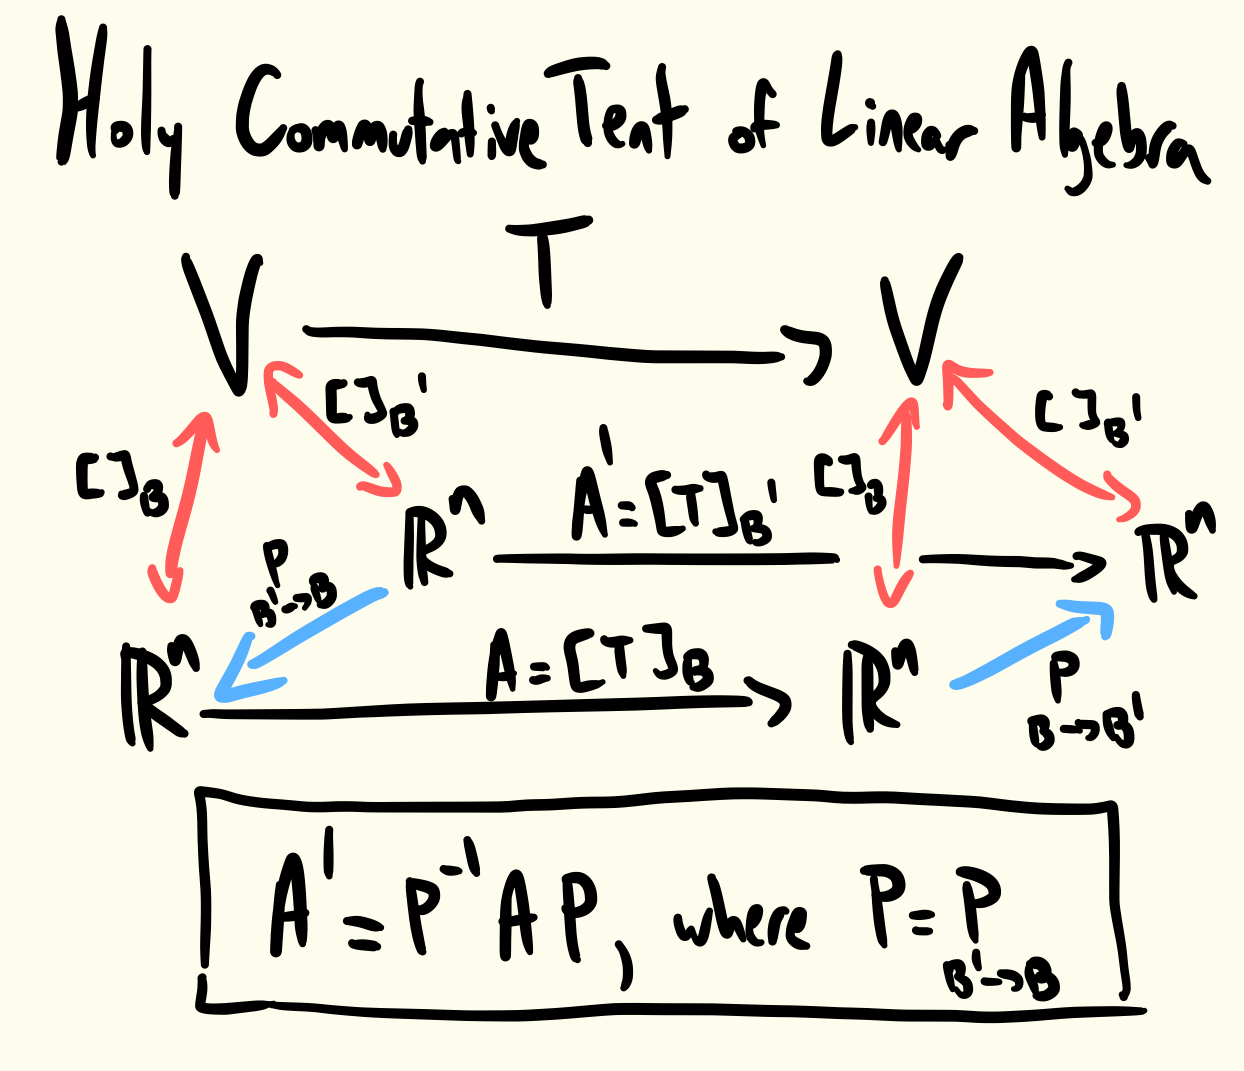
\includegraphics[width=4in]{Images/HolyCommutativeTent}

\end{frame}

\subsection{Eigenvectors and eigenvalues}
%\begin{frame}<beamer>
%             \frametitle{Outline}
%             \begin{multicols}{2}
%             \tableofcontents[currentsection,currentsubsection]
%             \end{multicols}{2}
%\end{frame}
%\begin{frame}{Eigenvectors}
Let $T\colon V\rightarrow V$ be linear. We have seen that some choices of bases of $V$ are better than others for representing $T$ as a matrix. 
\bpause
The ideal situation is when $V$ happens to have a basis $B=\{\boldv_1,\dots, \boldv_n\}$ where $T(\boldv_i)=c_i\boldv_i$ for all $i$. The matrix $[T]_B$ in this case is diagonal!
\[
[T]_B=\begin{bmatrix}
c_1&0&\dots\\
0&c_2&0&\dots\\
\vdots &\\
0&0&\dots&c_n
\end{bmatrix}
\]  
\pause This motivates us to find as many vectors as we can satisfying $T(\boldv)=c\boldv$ for some $c$. Such vectors are called \alert{eigenvectors}.
\begin{definition}
Let $T\colon V\rightarrow V$ be linear. An {\bf eigenvector} of $T$ is a \alert{nonzero} vector $\boldv\ne\boldzero$ such that $T(\boldv)=\lambda\boldv$ for some constant $\lambda\in\R$.  
\end{definition}
\pause 
\alert{Comment:} why the switch to $\lambda$ all of a sudden? Tradition!  
\end{frame}
\begin{frame}{Examples by inspection}
Define $T\colon M_{22}\rightarrow M_{22}$ as $T(A)=A^T+A$. 

We have seen that 
\begin{eqnarray*}
T\left(\begin{bmatrix}[rr]
0&1\\
-1&0
\end{bmatrix}
\right)&=&\begin{bmatrix}[rr]
0&0\\
0&0
\end{bmatrix}=0\begin{bmatrix}[rr]
0&1\\
-1&0
\end{bmatrix}\\
T\left(\begin{bmatrix}[rr]
0&1\\
1&0
\end{bmatrix}
\right)&=&\begin{bmatrix}[rr]
0&2\\
2&0
\end{bmatrix}=2\begin{bmatrix}[rr]
0&1\\
1&0
\end{bmatrix}.
\end{eqnarray*}

\pause Thus $\begin{bmatrix}[rr]
0&1\\
-1&0
\end{bmatrix}$
is an eigenvector with eigenvalue 0, and $\begin{bmatrix}[rr]
0&1\\
1&0
\end{bmatrix}$ is an eigenvector with eigenvalue 2. 
\end{frame}
\begin{frame}{Examples by inspection}
Let $T_\theta\colon\R^2\rightarrow\R^2$ be rotation counterclockwise by $\theta$, $0<\theta<2\pi$.  

What are the eigenvectors/eigenvalues of $T_\theta$. (Think geometrically, do not use a matrix representation of $T_\theta$!)
\begin{bsolution}
Is there any vector $\boldv$ such that when we rotate it by $\theta$ we get a scalar multiple of $\boldv$?
\bspace
Our answer actually depends on exactly what $\theta$ is. 

If $\theta=\pi$, then $T_\pi$ is rotation by 180$^\circ$, and so $T_\pi(\boldv)=-\boldv$ for all $\boldv$. Thus everything is an eigenvector of $T_\pi$ with eigenvalue $-1$. 
\bspace
If $\theta\ne\pi$, then we see easily that $T_\theta$ has no eigenvectors. 
\end{bsolution}
\end{frame}
\begin{frame}{Examples by inspection}
Fix $\alpha$ with $0\leq \alpha<\pi$, let $\ell_\alpha$ be the line making an angle $\alpha$ with the positive $x$-axis, and let $T_\theta\colon\R^2\rightarrow\R^2$ be reflection through $\ell_\alpha$.

What are the eigenvectors/eigenvalues of $T_\alpha$. (Think geometrically, do not use a matrix representation of $T_\alpha$!)
\begin{bsolution}
If $\boldv$ lies along $\ell_\alpha$ to begin with, then its reflection through $\ell_\alpha$ is itself. This means $T_\alpha(\boldv)=\boldv$. Thus all vectors along $\ell_\alpha$ are eigenvectors with eigenvalue 1. 
\bspace
If $\boldv$ lies along the line perpendicular to $\ell_\alpha$, then its reflection is just $-\boldv$ (draw a picture). Thus all vectors along this line are eigenvectors with eigenvalue $-1$. 
\bspace 
Vectors pointing along any other line will not be eigenvectors. Draw a picture!

\end{bsolution}
\end{frame}
\begin{frame}{Finding eigenvalues of $T$ systematically}
Let $T\colon V\rightarrow V$ be linear, $\dim(V)=n$. 

Our first step for finding eigenvalues and eigenvectors of $T$ is to 
pick a basis $B$ for $V$ and represent $T$ with the matrix $A=[T]_B$.  
\bpause You get to choose the basis $B$ yourself, though typically we start with the standard basis of $V$. It is usually only after our eigenvector analysis that we can provide a cleverer choice of basis. 
\bpause
Once we have chosen an $A$ to represent $T$, we perform our analysis on $A$. As usual, anything we discover about $A$ will be true of $T$. For example:
\bb
\ii $A$ and $T$ have precisely the same eigenvalues.
\ii Eigenvectors of $A$ can be translated back to $V$ to get eigenvectors of $T$. 
\ee
\end{frame}
\begin{frame}{Finding eigenvalues of $A$}
\footnotesize
We now focus on finding eigenvalues of an $n\times n$ matrix $A$. Follow this chain of equivalences:
\begin{eqnarray*}
\text{$\lambda\in\R$ is an eigenvalue of $A$}&\Leftrightarrow&
\pause A\boldx=\lambda\boldx \text{ for some $\boldx\ne 0$}
\ \text{ (by def.)}\\
\pause&\Leftrightarrow&\lambda\boldx-A\boldx=\boldzero\\
\pause&\Leftrightarrow&(\lambda I_n)\boldx-A\boldx=\boldzero \ \text{ (since $\lambda\boldx=(\lambda I_n)\boldx$)}\\
\pause&\Leftrightarrow&(\lambda I_n-A)\boldx=\boldzero \text{ for some $\boldx\ne \boldzero$}\\
\pause&\Leftrightarrow&\lambda I_n-A \text{ is noninvertible}\\
\pause&\Leftrightarrow&\det(\lambda I_n-A)=0 \ \text{ (invertibility theorem)}
\end{eqnarray*}
\pause 
Thus we see that $\lambda$ is an eigenvalue if and only if $\det(\lambda I_n-A)=0$. 
\bpause 
Set $p(t)=\det(tI_n-A)$. This is polynomial function in $t$, as you will see shortly. We have just shown that the eigenvalues of $A$ are precisely the \alert{real roots} of $p(t)$. Better give this important object a name!
\pause
\begin{definition}
Let $A$ be $n\times n$. The {\bf characteristic polynomial} of $A$ is the polynomial 
\[
p(t)=\det(tI_n-A).
\]
\end{definition}
\end{frame}
\begin{frame}
\alert{Example}. Find all eigenvalues of $A=\begin{bmatrix}
1&1\\
2&-1
\end{bmatrix}$. 
\begin{bsolution}
Compute:

$
p(t)=\det(tI-A)=\val{\begin{array}{cc}t-1&-1\\ -2&t+1 \end{array}}=t^2-3.
$

\pause The eigenvalues are the roots of $p(t)$: $
\lambda_1=\sqrt{3}, \lambda_2=-\sqrt{3}$.
\end{bsolution}

\pause
\alert{Example}. Find all eigenvalues of $A=\begin{bmatrix}[rrr]
2&-1&-1\\
-1&2&-1\\
-1&-1&2
\end{bmatrix}$.
\begin{bsolution}
Compute:

$
p(t)=\det(tI-A)=\val{\begin{array}{ccc}t-2&1&1\\ 1&t-2&1\\ 1&1&t-2 \end{array}}=t^3-6t^2+9t=t(t-3)^2.
$

\pause The eigenvalues are the roots of $p(t)$: $\lambda_1=0$, $\lambda_2=3$.
\end{bsolution}
\end{frame}
\begin{frame}{Facts about the characteristic polynomial}
%\footnotesize
Let $A$ be $n\times n$ and let $p(t)=\det(tI-A)$ be the characteristic polynomial. 
\bb
\pause\ii $p(t)=t^n+a_{n-1}t^{n-1}+\cdots +a_1t+a_0$; in particular, $p(t)$ is {\em monic} (leading coefficient is 1), of degree $n$. 
\pause\ii  $p(t)$ has at most $n$ distinct roots. Some of these roots may be complex. Thus it is possible to have less than $n$ eigenvalues. Indeed, there may be no eigenvalues. 
\bpause 
What about the possible complex roots? Let's call these \alert{complex eigenvalues}. For now they do not count as eigenvalues for us, as it is impossible to find a nonzero $\boldx\in\R^n$ with a complex eigenvalue. 

\ee
\end{frame}
\begin{frame}{Fancy facts about $p(t)$}
\footnotesize
Let $p(t)=\det(tI-A)=t^n+a_{n-1}t^{n-1}+\cdots +a_1t+a_0$ be the characteristic polynomial. \\
Over $\C$ we can factor $p(t)=(t-\lambda_1)(t-\lambda_2)\cdots (t-\lambda_n)$, where some of the $\lambda_i$ may be complex numbers. 
\bpause Then we have: 
\begin{eqnarray*}
-(\lambda_1+\lambda_2+\cdots +\lambda_n)&=&a_{n-1}=-\tr(A)\\
(-1)^n\lambda_1\lambda_2\cdots\lambda_n&=&a_0=(-1)^n\det(A)
\end{eqnarray*}
\pause An easy consequence of these equalities is the following:
\begin{eqnarray*}
\tr(A)&=&\lambda_1+\lambda_2+\cdots +\lambda_n\\
\det(A)&=&\lambda_1\lambda_2\cdots\lambda_n
\end{eqnarray*}
In plain English: $\tr(A)$ is the sum of the eigenvalues; $\det(A)$ is the product of the eigenvalues. 
\bpause 
When $A$ is $2\times 2$, the above implies $p(t)=t^2-\tr(A)t+\det(A)$: a useful shortcut when having to compute eigenvalues of $2\times 2$ matrices! 
\end{frame}
\begin{frame}
 Let's make our list of facts official. 
 \begin{theorem}[Characteristic polynomial theorem]
 Let $A\in M_{nn}$, and let $p(t)=\det(tI_n-A)$ be its characteristic polynomial. 
 \bb[(a)]
 \ii $p(t)=t^n+a_{n-1}t^{n-1}+\cdots +a_1t+a_0$; in particular, $p(t)$ is {\em monic} (leading coefficient is 1), of degree $n$. 
 \ii The real roots of $p(t)$ are the (real) eigenvalues of $A$. Since $\deg p(t)=n$, there are at most $n$ distinct eigenvalues of $A$. 
 \ii Let $\lambda_1, \lambda_2, \dots, \lambda_n$ be the roots of $p(t)$. Then 
 \begin{align*}
 \tr(A)&=\sum_{i=1}^n\lambda_i=-a_{n-1}\\
 \det(A)&=\prod_{i=1}^n\lambda_i=(-1)^na_0
 \end{align*}
 \ee
 \end{theorem}
\end{frame}
\begin{frame}{Finding eigenvectors of $A$}
Now suppose we have found an eigenvalue $\lambda$ of $A$. 
\\
Our chain of equivalences from earlier told us that the eigenvectors of $A$ with eigenvalue $\lambda$ are precisely the \alert{nonzero} solutions to the matrix equation $(\lambda I_n-A)\boldx=\boldzero$. 
\bpause 
Thus to find all eigenvectors with eigenvalue $\lambda$ we simply compute $\NS(\lambda I_n-A)$ using Gaussian elimination.
\pause
\begin{definition}
Let $\lambda$ be an eigenvalue of $A$. We define the $\lambda$-eigenspace of $A$ to be the space 
\[
W_\lambda:=\NS(\lambda I_n-A).
\]
The nonzero elements of $W_\lambda$ are precisely the eigenvectors of $A$ with eigenvalue $\lambda$. 
\end{definition}
\end{frame}
\begin{frame}
Let's compute the eigenspaces of our previous examples. 

\alert{Example}. $A=\begin{bmatrix}
1&1\\
2&-1
\end{bmatrix}$, $\lambda_1=\sqrt{3}$, $\lambda_2=-\sqrt{3}$.
\begin{bsolution}
\pause Compute:

$W_{\sqrt{3}}=\NS(\sqrt{3}I-A)=\NS\left(\begin{bmatrix}\sqrt{3}-1&-1\\ -2&\sqrt{3}+1 \end{bmatrix}\right)\pause=\Span(\left\{ \begin{bmatrix}\sqrt{3}+1\\2\end{bmatrix} \right\})$

\pause
$W_{-\sqrt{3}}=\NS(-\sqrt{3}I-A)=\NS\left(\begin{bmatrix}-\sqrt{3}-1&-1\\ -2&-\sqrt{3}+1 \end{bmatrix}\right)\pause=\Span(\left\{ \begin{bmatrix}-\sqrt{3}+1\\ 2\end{bmatrix} \right\})$
\bpause Thus any multiple of $\boldv_1=(\sqrt{3}+1,2)$ is an eigenvector of $A$ with eigenvalue $\sqrt{3}$, and any multiple of $\boldv_2=(-\sqrt{3}+1,2)$ is an eigenvector of $A$ with eigenvalue $-\sqrt{3}$. 
\bpause
Check:
\bspace
$A\begin{bmatrix}\sqrt{3}+1\\ 2 \end{bmatrix}=\begin{bmatrix} 3\sqrt{3}+3\\ 2\sqrt{3} \end{bmatrix}=\sqrt{3}\begin{bmatrix}\sqrt{3}+1\\ 2 \end{bmatrix} \checkmark$. 
\bspace
$A\begin{bmatrix}-\sqrt{3}+1\\ 2 \end{bmatrix}=\begin{bmatrix} -3\sqrt{3}+3\\ -2\sqrt{3} \end{bmatrix}=-\sqrt{3}\begin{bmatrix}-\sqrt{3}+1\\ 2 \end{bmatrix} \checkmark$. 

\end{bsolution}
\end{frame}
\begin{frame}
Let's compute the eigenspaces of our previous examples. 

\alert{Example}. $A=\begin{bmatrix}[rrr]
2&-1&-1\\
-1&2&-1\\
-1&-1&2
\end{bmatrix}$, $\lambda_1=0$, $\lambda_2=3$. 
\begin{bsolution}
Compute:

$W_0=\NS(0I-A)=\NS\left(\begin{bmatrix}[rrr]
2&-1&-1\\
-1&2&-1\\
-1&-1&2
\end{bmatrix}
\right)=\Span\left(\left\{\boldv_1=\begin{bmatrix}1 \\ 1 \\ 1 \end{bmatrix}\right\}\right)$. 
\bpause
$W_3=\NS(3I-A)=\NS(\left( \begin{bmatrix} 1&1&1\\ 1&1&1\\ 1&1&1   \end{bmatrix} \right)
=\Span\left(\left\{\boldv_2= \begin{bmatrix}[r] 1 \\ -1 \\ 0 \end{bmatrix}, \boldv_3=\begin{bmatrix}[r]1 \\ 0 \\ -1 \end{bmatrix}\right\}\right)$. 
\bpause
Thus the eigenvectors of $A$ with eigenvalue 0 are vectors of the form $c\boldv_1$, and the eigenvectors of $A$ with eigenvalue 3 are vectors of the form $c\boldv_2+d\boldv_3$. 

\bpause\alert{Comment}. Note that in general $W_0=\NS(0I-A)=\NS(-A)=\NS(A)$. (Think about why the last equality is true.) 

Thus the eigenvectors of $A$ with eigenvalue 0 are precisely the nonzero vectors of $\NS(A)$, should there be any at all!  
\end{bsolution}
\end{frame}


\subsection{Diagonalization}
\begin{frame}<beamer>
             \frametitle{Outline}
             \begin{multicols}{2}
             \tableofcontents[currentsection,currentsubsection]
             \end{multicols}{2}
\end{frame}
\begin{frame}{Diagonalizable matrices}
\begin{definition}
An $n\times n$ matrix $A$ is {\bf diagonalizable} if there is an invertible matrix $P$ such that $D=P^{-1}AP$ is diagonal. 

In other words, $A$ is diagonalizable if it is \alert{similar} to a diagonal matrix $D$. 
\end{definition}
 \pause
 \begin{comments}
 \bb
 \ii If $A$ is itself diagonal, then it is diagonalizable: we may choose $P=I_n$ in the definition. 
 \pause\ii In this section we will develop a systematic procedure for determining whether a matrix is diagonalizable. As we will see, the answer is yes if and only if $A$ has ``enough" linearly independent eigenvectors. Of course we will spell out precisely what we mean by ``enough". 
 \pause\ii Not all matrices are diagonalizable. For example, $A=\begin{bmatrix}
 0&1\\
 0&0
 \end{bmatrix}$ is not diagonalizable, as the aforementioned procedure will show. 
 \pause\ii Roughly speaking, you should interpret being diagonalizable as meaning ``as good as diagonal". To elaborate: doing arithmetic with diagonal matrices $D$ is extremely easy; if we know $A$ is diagonalizable, meaning it is similar to a diagonal matrix $D$, then it shares many essential properties of $D$, and we can use the relation $D=P^{-1}AP$ to help ease arithmetic computations involving $A$.   \ee
 \end{comments}
\end{frame}
\begin{frame}{Properties of conjugation}
If we have, $D=P^{-1}AP$, why exactly is there such a close connection between $D$ and $A$? One explanation has to do with the underlying operation  
\[
A\longmapsto P^{-1}AP,
\]
which we call \alert{conjugation by $P$}.  As the following theorem outlines, conjugation by an invertible $P$ satisfies many useful properties, and we use these to relate the matrix $A$ with the matrix $P^{-1}AP$. 
\pause
\begin{theorem}[Properties of conjugation]\label{th:conjugation}
Let $P$ be any invertible $n\times n$ matrix. 
\bb
\ii $P^{-1}(c_1A_1+c_2A_2)P=c_1P^{-1}A_1P+c_2P^{-1}A_2P$. (\alert{Conjugation by $P$ is a linear transformation}.) 
\ii $P^{-1}A^nP=(P^{-1}AP)^n$ for any integer $n\geq 0$. If $A$ is invertible, the equality holds for {\em all} integers $n$. (\alert{Conjugation preserves powers}.) 
\ii Recall that given any polynomial $f(x)=\anpoly$ and any $n\times n$ matrix $A$ we define $f(A)=a_nA^n+a_{n-1}A^{n-1}+a_1A+a_0I_n$. 

We have $f(P^{-1}AP)=P^{-1}f(A)P$ for any polynomial $f(x)$, and any $n\times n$ matrix $A$. (\alert{Conjugation preserves polynomial evaluation}.) 
\ee
\end{theorem}
\pause
\begin{proof}
Exercise.
\end{proof}
\end{frame}
\begin{frame}{Examples: utility of diagonalizability}
Suppose $A$ is diagonalizable, so that $D=P^{-1}AP$, where $D$ is diagonal with diagonal entries $d_i$. Using Theorem \ref{th:conjugation}, we can now see how to translate statements about $D$ (which are generally easy to prove), to statements about $A$ (which otherwise might have been difficult to show). 
\begin{example}\label{eg:diagpowers}
To compute $A^{n}$ (hard) we can just compute $D^{n}$ (easy) and then observe that $A=PDP^{-1}$, and thus 
\[
A^{n}=(PDP^{-1})^{n}=PD^{n}P^{-1},
\] 
where the last equality follows from part (b) of Theorem \ref{th:conjugation}; here we let $P^{-1}$ assume the role of $P$ in the theorem statement. 
\bpause
For example, let $A=\begin{bmatrix}
1&3\\
1&-1
\end{bmatrix}$. Let's compute $A^n$ for arbitrary $n$. 

We have $D=P^{-1}AP$, where $D=\begin{bmatrix}[rr]
2&0\\
0&-2
\end{bmatrix}$, and $P=\begin{bmatrix}[rr]
3&1\\
1&-1
\end{bmatrix}$. (This is not obvious yet. Soon we will have the tools to see why this is so.)
\bpause 
Then $A=PDP^{-1}$, and thus 
\[
A^{n}=PD^{n}P^{-1}=P\begin{bmatrix}
2^{100}&0\\
0&(-2)^{100}
\end{bmatrix}P^{-1}=\frac{1}{4}\begin{bmatrix}
3\cdot2^n+(-2)^n&3\cdot 2^n-3(-2)^{n}\\
2^{n}-(-2)^n&2^n+3(-2)^{n}
\end{bmatrix}.
\] 
\end{example}

\end{frame}
\begin{frame}{Examples: utility of diagonalizability}
Suppose $A$ is diagonalizable, so that $D=P^{-1}AP$, where $D$ is diagonal with diagonal entries $d_i$. 
\begin{example}
More generally, we have $f(A)=f(PDP^{-1})=Pf(D)P^{-1}$ for any polynomial $f(x)=\anpoly$. Since $D$ is diagonal, with diagonal entries $d_i$, it is easy to see that $f(D)$ is also diagonal, with diagonal entries $f(d_i)$. 
\bpause
In particular we see that $f(A)=\underset{n\times n}{\boldzero}$ if and only if $f(D)=\underset{n\times n}{\boldzero}$, and this holds if and only if $f(d_i)=0$ for each diagonal entry $d_i$ of $D$.  
\bpause
Take the matrix $A$ from Example \ref{eg:diagpowers}, and let $f(x)=(x-2)(x+2)=x^2-4$. Since $f(2)=f(-2)=0$, it follows that $f(D)=f(A)=\underset{2\times 2}{\boldzero}$. In other words, $A^2-4I=\underset{2\times 2}{\boldzero}$, as you can easily check. 

\end{example}
\end{frame}
\begin{frame}{Examples: utility of diagonalizability}
Suppose $A$ is diagonalizable, so that $D=P^{-1}AP$, where $D$ is diagonal with diagonal entries $d_i$. 
\begin{example}
$A$ has a \alert{square-root} (i.e., a matrix $B$ such that $B^2=A$) iff $D$ has a square-root. 
\bpause Indeed, suppose $B^2=A$. Set $C=P^{-1}BP$. Then $C^2=P^{-1}B^2P=P^{-1}AP=D$. Similarly, if $C^2=D$, then $B^2=A$, where $B=PCP^{-1}$. 
\bpause
As an example,  the matrix $A=\begin{bmatrix}
0&-2\\
1 &3
\end{bmatrix}$, satisfies $D=P^{-1}AP$, where $D=\begin{bmatrix}
1&0\\
0&2
\end{bmatrix}$, and $P=\begin{bmatrix}
2&1\\
-1&-1
\end{bmatrix}$. Since $C=\begin{bmatrix}
1&0\\
0&\sqrt{2}
\end{bmatrix}$ is a square-root of $D$, $B=PCP^{-1}=\begin{bmatrix}
2-\sqrt{2}&2-2\sqrt{2}\\
-1+\sqrt{2}&-1+2\sqrt{2}
\end{bmatrix}$ is a square-root of $A$, as you can easily check. 
\bpause
So when exactly does a diagonal matrix $D$ have a square-root? Clearly, it is sufficient that $d_i\geq 0$ for all $i$, as in the example above. Interestingly, this is not a necessary condition! Indeed, consider the following example: 

$
\begin{bmatrix}[rr]
-1&0\\
0&-1
\end{bmatrix}=\begin{bmatrix}[rr]
0&-1\\
1&0
\end{bmatrix}^2.
$ 
\end{example}
\end{frame}

\begin{frame}{Properties of similarity}
Before investigating the question of when a matrix is diagonalizable, we record a few more properties illustrating the close connection between similar matrices. 
\begin{theorem}[Properties of similarity]\label{th:similarity}
Suppose $A$ is similar to $B$: i.e., there is an invertible matrix $P$ such that $B=P^{-1}AP$. Then:
\bb[(a)]
\ii $B$ is similar to $A$. (\alert{Similarity is symmetric}.)
\ii $A$ and $B$ have the same trace and determinant. 
\ii $A$ and $B$ have the same rank. 
\ii $A$ and $B$ have the same characteristic polynomial.  
\ii $A$ and $B$ have the same eigenvalues. 
\ii Given any $\lambda\in\R$, let $W_\lambda$ be the corresponding eigenspace for $A$, and $W_\lambda'$ the corresponding eigenspace for $B$. Then $\dim W_{\lambda}=\dim W_{\lambda}'$. 
\ee
\end{theorem}
\pause The proof of (d) follows. I leave the rest as an exercise. 
\end{frame}
\begin{frame}
\begin{proof}[Proof of Theorem \ref{th:similarity}.d]
By definition we have $B=P^{-1}AP$ for some matrix $P$. We wish to show the characteristic polynomials $p_A(t)$ and $p_B(t)$ of the two matrices are equal. Compute:  
\begin{eqnarray*}
p_B(t)&=&\det(tI-B)\\
\pause &=&\det(tI-P^{-1}AP) \\
\pause &=&\det(tP^{-1}IP-P^{-1}AP) \ \text{ (since $P^{-1}IP=I$)} \\
\pause &=&\det(P^{-1}tIP-P^{-1}AP) \ \text{ ($t$ behaves as scalar)} \\
\pause &=&\det(P^{-1}(tI-A)P) \\
\pause &=&\det(P^{-1})\det(tI-A)\det(P)\\
\pause &=&(\det(P))^{-1}\det(P)\det(tI-A)\\
\pause &=&\det(tI-A)=p_A(t). 
\end{eqnarray*}
\end{proof}
\end{frame}
\begin{frame}{The true meaning of similarity}
Hopefully Theorems \ref{th:conjugation} and \ref{th:similarity} convince you that similar matrices (in the linear algebraic sence) are truly similar (in the usual sense). 
\bpause
There is, however, a deeper explanation for this. Namely, if $A$ and $A'$ are similar, then they are simply two different matrix representations of a common linear transformation!
\pause

In more detail: suppose we have $A'=P^{-1}AP$. 
\begin{itemize}
\ii Let $B$ be the standard basis of $\R^n$, and let $B'$ be the basis of $\R^n$ obtained by taking the columns of the invertible matrix $P$. Finally, let $T=T_A$ be the matrix transformation associated to $A$. 
\ii Then $A=[T]_B$, $P=\underset{B'\rightarrow B}{P}$, and $P^{-1}=\underset{B\rightarrow B'}{P}$. 
\ii From the change of basis formula it follows that 
\[
A'=P^{-1}AP=\underset{B\rightarrow B'}{P}[T]_B\underset{B'\rightarrow B}{P}=[T]_{B'}
\]
\end{itemize}
\bpause
In other words to say $A$ and $A'$ are similar is simply to say that they are different matrix representations of the same overlying linear transformation $T$ (see Holy Commutative Tent of Linear Algebra on next slide). All their shared properties (same eigenvalues, same determinant, same trace, etc.) are simply the properties they inherit from this one overlying $T$, of which they are but earthly shadows. 
\bpause
There is one true $T$!
\end{frame}
\begin{frame}
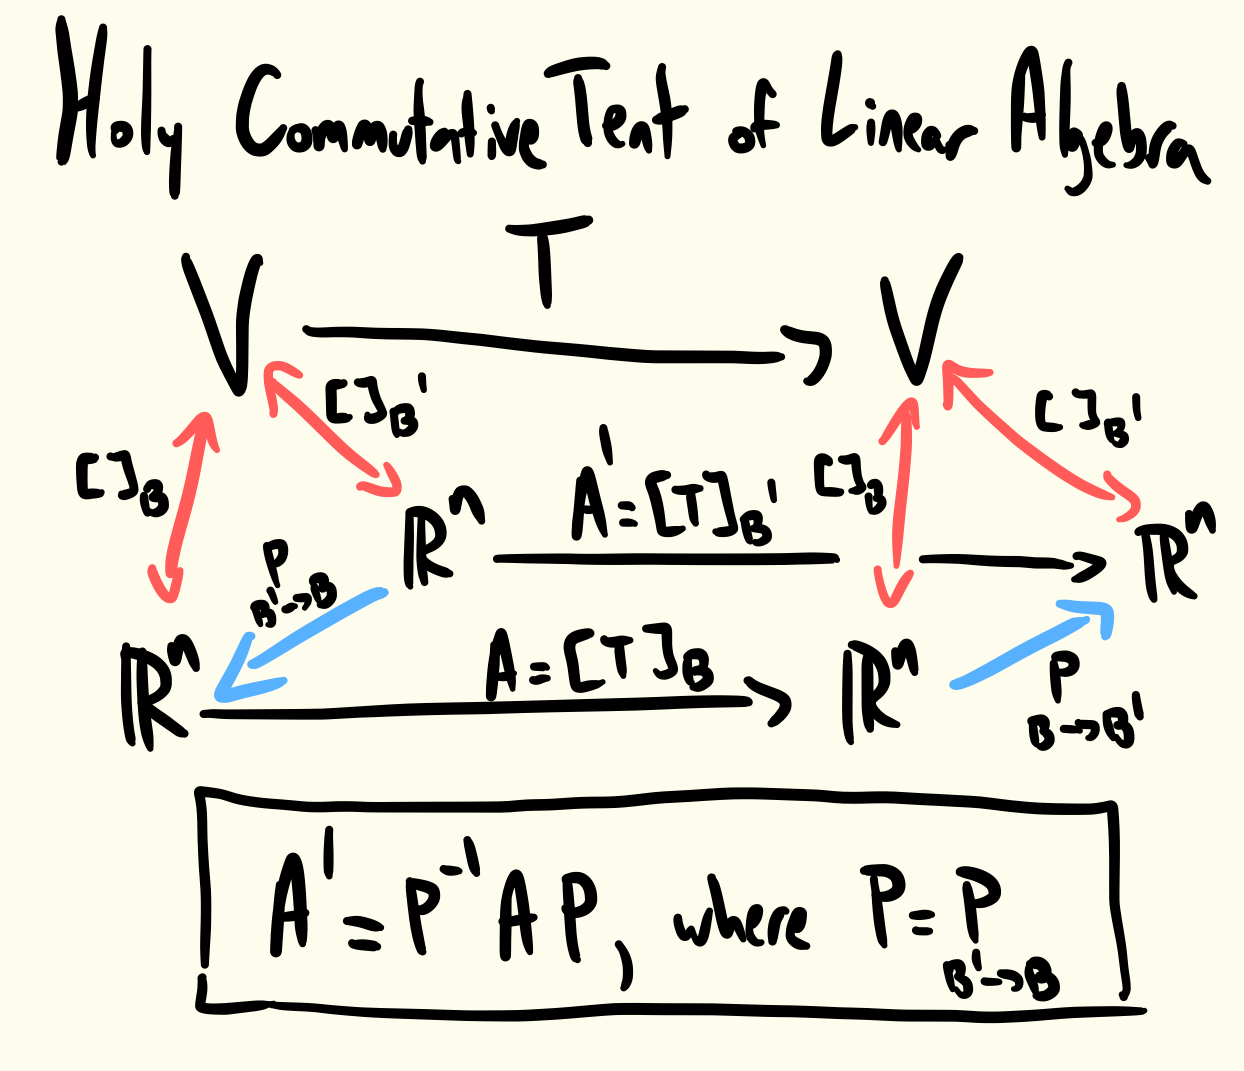
\includegraphics[width=4.5in]{Images/HolyCommutativeTent}

\end{frame}

%\begin{frame}
%\alert{Theorem (Holy commutative tent of linear algebra)}
%The following statements are equivalent:
%
%\alert{(i)} $A$ and $A'$ are similar. 
%
%\alert{(ii)} There is a linear $T\colon V\rightarrow V$ and bases $B$, $B'$ of $V$ such that $A=[T]_B$, $A'=[T]_{B'}$. 
%
%Furthermore, in this situation we have $A'=P^{-1}AP$, where $P=\underset{B'\rightarrow B}{P}$. 
%\pause
%\begin{proof}
%\alert{(ii)$\Rightarrow$ (i)}. 
%Suppose $A=[T]_B$ and $A'=[T]_{B'}$ are two different matrix representations of $T$. Then 
%the change of basis for transformations theorem ( \ref{Th:changeofbasis}) tells us that 
%$
%A'=(P_{B' \rightarrow B})^{-1}AP_{B' \rightarrow B}.
%$
%Thus $A$ and $A'$ are similar. 
%
%\bpause
%\alert{(i)$\Rightarrow$(ii)}. 
%Suppose $A=P^{-1}A'P$. Set $T=T_{A}$, let $B$ be the standard basis of $\R^n$ and let $B'$ be the basis we get by taking the columns of $P$. Then $P=\underset{B'\rightarrow B}{P}$ and $P^{-1}=\underset{B\rightarrow B'}{P}$. 
%
%It is clear with this setup that $A=[T]_B$, since $B$ is the standard basis. Using the relation $A'=P^{-1}AP$ and the  change of basis for transformations theorem ( \ref{Th:changeofbasis}), we have $A'=[T]_{B'}$. 
%\end{proof}
%\end{frame}
\begin{frame}
\footnotesize
The previous theorem allows us to extend some of our matrix definitions to linear transformations. 
\begin{definition}
Let $T\colon V\rightarrow V$ be linear, let $B$ be \alert{any basis} of $V$, and let $A=[T]_B$. We  define
the {\bf characteristic polynomial} of $T$ to be $p(t)=\det(tI-A)$. 
\end{definition}
\pause
\begin{comment}
Note that the characteristic polynomial defined above does not depend on the choice of basis $B$. If $B'$ is another basis, and $A'=[T]_{B'}$, then $A'$ and $A$ are similar, as we have seen, and thus have the same characteristic polynomial. 
\end{comment}
\pause
\begin{definition}
A linear transformation $T\colon V\rightarrow V$ is {\bf diagonalizable} if there exists a basis $B$ of $V$ for which $[T]_B$ is a diagonal matrix. 
\end{definition}
 \pause
 \begin{comment}
Equivalently, $T$ is diagonalizable if for \alert{any} choice of basis $B$ the matrix $[T]_B$ is diagonal\alert{izable}.  
 \end{comment}
 \end{frame}
\begin{frame}{Diagonalizability and eigenvectors}
At last we relate the property of being diagonalizable with the notion of eigenvectors. In the process we make clear what we mean when we say $T$ is diagonalizable if and only if it has ``enough" linearly independent eigenvectors. 
\pause
\begin{theorem}[Diagonalizability theorem]\label{th:diagonalizability}
Let $T\colon V\rightarrow V$ be linear, $\dim(V)=n$.
\bb
\ii (\alert{Qualitative}) Given basis $B$ of $V$, the matrix $[T]_B$ is diagonal if and only if $B$ consists of eigenvectors of $T$. 

Thus $T$ is diagonalizable if and only if there is a basis of $V$ consisting of eigenvectors of $T$. 
\ii (\alert{Quantitative}) Let $\lambda_1, \lambda_2, \dots, \lambda_r$ be the \alert{distinct} eigenvalues of $T$, let $W_{\lambda_j}$ be the corresponding eigenspaces, and let $n_j=\dim W_{\lambda_j}$. 

Then $T \text{ is diagonalizable}\Longleftrightarrow n_1+n_2+\cdots +n_r=n$.
\ee
\end{theorem}
\pause
\begin{proof}
The first statement was a homework exercise. The proof of the second statement is within our means, but somewhat lengthy. I will sketch its proof elsewhere.  For now it is more important to understand how to use the result. 
\end{proof}
\end{frame}

\begin{frame}{Deciding whether $T\colon V\rightarrow V$ is diagonalizable}
Suppose $\dim(V)=n$. 
\bb
\ii Pick a basis $B$ of $V$. Set $A=[T]_B$
\pause\ii Find the distinct eigenvalues, $\lambda_1,\dots, \lambda_r$,  of $A$, let $W_{\lambda_i}$ be the corresponding eigenspaces, and let $n_i=\dim W_{\lambda_i}$.
\pause\ii $A$ (and thus $T$) is diagonalizable if and only if 
$
n_1+n_2+\cdots +n_r=n.
$ 
\pause\ii If the above equality is true, compute bases for each $W_{\lambda_i}$ in $\R^n$. 
\pause\ii Lift all vectors from all these bases back to $V$ using $[\hspace{5pt}]_B$. This is a new basis $B'$ of $V$ consisting of eigenvectors of $T$. 
\pause\ii $[T]_{B'}=D$ is diagonal. 
\ee

\end{frame}
\begin{frame}{Deciding whether $A_{n\times n}$ is diagonalizable}
\bb
\ii Find the distinct eigenvalues, $\lambda_1,\dots, \lambda_r$,  of $A$, let $W_{\lambda_i}$ be the corresponding eigenspaces, and let $n_i=\dim W_{\lambda_i}$.
\pause\ii $A$ is diagonalizable if and only if 
$
n_1+n_2+\cdots +n_r=n.
$ 
\pause\ii If the above equality is true, compute bases $B_j$ for each $W_{\lambda_j}$. 
\pause\ii Place all the vectors from the bases $B_j$ as columns of a matrix $P$. As these eigenvectors are linearly independent, $P$ is invertible.  
\pause\ii The matrix $D=P^{-1}AP$ is diagonal. 

In more detail, the $j$-th diagonal entry of $D$ is the eigenvalue associated to the eigenvector in the $j$-th column of $P$. This means the first $n_1$ diagonal entries of $D$ are equal to $\lambda_1$, the next $n_2$ entries are equal to $\lambda_2$, etc. 
\ee

\end{frame}
\begin{frame}{Example}
Take $A=\begin{bmatrix}
1&1\\
0&1
\end{bmatrix}$. Earlier I claimed that this matrix is not diagonalizable. Let's see why.
\bpause
The characteristic polynomial of $A$ is $p(t)=(t-1)^2$. Thus $\lambda=1$ is the only eigenvalue of $A$. 
\bpause
We have $W_1=\NS(I-A)=\NS\begin{bmatrix}
0&-1\\
0&0
\end{bmatrix}$. We see clearly that $\rank(I-A)=1$, and hence $\dim W_1=\dim\NS(I-A)=2-1=1$. 
\bpause
Since $W_1$ is the only eigenspace, and since $\dim W_1=1\ne 2$, we conclude $A$ is not diagonalizable. 
\end{frame}
\begin{frame}{Example}
Let $A=\begin{bmatrix}[rrrr]
14 & 21 & 3 & -39 \\
12 & 25 & 3 & -41 \\
12 & 24 & 5 & -42 \\
12 & 22 & 3 & -38
\end{bmatrix}$.  
\bpause
The characteristic polynomial of $A$ is $p(t)=x^4 - 6x^3 + 9x^2 + 4x - 12$. (This is not obvious, but would be a pain to compute in detail. You may take this for granted.) 
\bpause
Our usual factoring tricks allow us to factor this as $p(x)=(x-2)^2(x+1)(x-3)$. 
\bpause
The eigenspaces are $W_2=\NS(2I-A), W_{-1}=\NS(-I-A)$, and $W_3=\null(3I-A)$. I'll leave it to you to verify that they have bases $B=\{ (3,2,0,2), (1,1,2,1)\}$, $B'=\{(1,1,1,1)\}$, and $B''=\{(3,5,6,4)\}$, respectively. 
\bpause
It follows that the dimensions of the eigenspaces are 2, 1, and 1, respectively. Since $2+1+1=4$, we conclude that $A$ is diagonalizable. 
\bpause
In more detail, we have $D=P^{-1}AP$, where 
\[
D=\begin{bmatrix}[rrrr]
2&0&0&0\\
0&2&0&0\\
0&0&-1&0\\
0&0&0&3
\end{bmatrix}, \ \
P=\begin{bmatrix}[rrrr]
3 & 1 & 1 & 3 \\
2 & 1 & 1 & 5 \\
0 & 2 & 1 & 6 \\
2 & 1 & 1 & 4
\end{bmatrix}
\]
\end{frame}

\begin{frame}{Geometric and algebraic multiplicity}
Take $A$ (or $T$) and suppose the characteristic polynomial $p(t)$ factors as 
\[
p(t)=(t-\lambda_1)^{n_1}(t-\lambda_2)^{n_2}\cdots (t-\lambda_r)^{n_r},
\]
where the $\lambda_i$ are the {\em distinct} eigenvalues of $A$ (or $T$). It turns out that the exponent $n_i$, called the {\bf algebraic multiplicity} of the eigenvalue $\lambda_i$, is an upper bound on $m_i=\dim W_{\lambda_i}$, called the {\bf geometric multiplicity}. 
\pause
\begin{theorem}[Algebraic and geometric multiplicity theorem]
Let $A$ (or $T$) have characterisitc polynomial 
\[
p(t)=(t-\lambda_1)^{n_1}(t-\lambda_2)^{n_2}\cdots (t-\lambda_r)^{n_r},
\]
where the $\lambda_i$ are the {\em distinct} eigenvalues of $A$ (or $T$). Then 
\[
\dim W_{\lambda_i}\leq n_i:
\]
i.e., the geometric multiplicity is less than or equal to the algebraic multiplicity. 
\end{theorem}
 
\end{frame}
\begin{frame}{Linear independence and eigenvectors}
The following result is used to prove the diagonalizability theorem (Theorem \ref{th:diagonalizability}), but is also very useful in its own right. 
\begin{theorem}\label{th:independentteigenvectors}
Let $T\colon V\rightarrow V$ be a linear transformation, and let $S=\{\boldv_1,\dots, \boldv_r\}$ be a set of eigenvectors of $T$ with $T\boldv_i=\lambda_i\boldv_i$. 

If the $\lambda_i$ are all distinct, then $S$ is linearly independent. 
\end{theorem}
\pause
\begin{proof}
Proved elsewhere.
\end{proof}
\pause
\begin{corollary}
Let $T\colon V\rightarrow V$ be a linear transformation, and suppose $\dim V=n$. 

If $T$ has $n$ \alert{distinct} eigenvalues, then $T$ is diagonalizable. 
\end{corollary}
\pause
\begin{proof}
Let $\boldv_1, \boldv_2,\dots, \boldv_n$ be eigenvectors corresponding to these $n$ distinct eigenvalues. The theorem tells us they form a linearly independent set. Since $\dim V=n$, they form a basis for $V$ by the dimension theorem compendium. Since $T$ has a basis of eigenvectors, it is diagonalizable. 
\end{proof}

\end{frame}
\begin{frame}
Theorem \ref{th:independentteigenvectors} makes no assumption about the dimension of $V$. It can thus be applied to interesting infinite-dimensional examples. 
\begin{example} 
Let $V=C^\infty(\R)$, and let $T\colon V\rightarrow V$ be defined as $T(f)=f'$. 

Let $f_i(x)=e^{k_ix}$, where the $k_i$ are all distinct constants. I claim $S=\{f_1,f_2,\dots , f_r\}$ is linearly independent. 
\bpause 
Indeed, each $f_i$ is an eigenvector of $T$, since $T(f_i)=(e^{k_ix})'=k_ie^{k_ix}=k_if_i$. 
\bpause 
Since the $k_i$'s are all distinct, it follows that the $f_i$ are eigenvectors with distinct eigenvalues, hence linearly independent!

\pause Note: try proving that $S$ is linearly independent using the the Wronskian! You get a very interesting determinant computation.  
\end{example}
\end{frame}
%\begin{frame}{Conditions guaranteeing diagonalizability}
%\begin{theorem}[Spectral Theorem]
%Let $A$ be a \alert{symmetric} $n\times n$ matrix, and let $p(x)$ be its characteristic polynomial. Then: 
%\bb[(i)]
%\ii $p(x)$ factors completely over the reals; 
%\ii $A$ is diagonalizable;
%\ii we can find an \alert{orthogonal} basis of eigenvectors of $A$.  
%\ee
%From (iii) it follows that we can find a matrix $Q$ with $Q^{-1}=Q^T$ such that 
%\[
%D=Q^{-1}AQ=Q^TAQ.
%\]
%\end{theorem}
%This is a fairly deep result with many important consequences in math and other fields. The proof is actually within our means at this point, but we will forgo it in consideration of time constraints. 
%\end{frame}
\begin{frame}{Final extension of the invertibility theorem}
Lastly, we can add one final statement to the invertibility theorem: $A$ is invertible if and only if $0$ is not an eigenvalue of $A$. 
\bpause 
Indeed $0$ is an eigenvalue of $A$ if and only if $p(0)=\det(0I-A)=\det(-A)=0$ if and only if $\det A=0$, since $\det(-A)=(-1)^n\det A$. \bpause
Since $\det A=0$ if and only if $A$ is not invertible, we conclude that $0$ is an eigenvalue of $A$ if and only if $A$ is not invertible.
\bpause
You find the final version of the invertibility theorem on the next slide. 
\end{frame}
\begin{frame}
\begin{theorem}[Invertibility theorem (final version)]
Let $A$ be $n\times n$. The following statements are equivalent. 
\bb[(a)]
\ii $A$ is invertible.
\ii $A\boldx=\boldzero$ has a unique solution (the trivial one). 
\ii $A$ is row equivalent to $I_n$, the $n\times n$ identity matrix.
\ii $A$ is a product of elementary matrices. 	
\ii $A\boldx=\boldb$ has a solution for every $n\times 1$ column vector $\boldb$. 
\ii $A\boldx=\boldb$ has a {\em unique} solution for every $n\times 1$ column vector $\boldb$. 
\ii $\det(A)\ne 0$.
\ii $\NS(A)=\{\boldzero\}$.
\ii $\nullity(A)=0$.
\ii $\rank(A)=n$. 
\ii $\CS(A)=\R^n$.
\ii $\RS(A)=\R^n$.
\ii The columns of $A$ are linearly independent (or span $\R^n$, or are a basis of $\R^n$).
\ii The rows of $A$ are linearly independent (or span $\R^n$, or are a basis of $\R^n$). 
%\ii The corresponding linear transformation $T_A$ is invertible. 
\ii $A$ does not have 0 as an eigenvalue. 
\ee
\end{theorem}

\end{frame}


\section{Inner product spaces}
\subsection{Inner products, norms, angles}
\begin{frame}{Inner product spaces}
We now define the notion of an inner product $\langle v,w \rangle$ on a vector space $V$. 
\bpause An inner product is an additional layer of structure added to the vector space operations defined on $V$. As with those operations, we define inner products \alert{axiomatically}. 
\bpause
The dot product operation defined on $\R^2$ and $\R^3$ serves as the basic model of an inner product; our axioms simply generalize prominent and useful properties of this particular inner product. 
\bpause
The main virtues of an inner product are:
\bb
\ii it allows us to define notions of orthogonality, distance and angle on $V$;
\ii it allows us to construct \alert{orthonormal} bases of $V$, which are computationally very easy to work with.  
\ee  
\end{frame}
\begin{frame}{Definition of inner product}
\begin{definition}
Let $V$ be a vector space. An {\bf inner product} on $V$ is an operation
\begin{align*}
\langle \ , \rangle \colon &V\times V\rightarrow \R \\
(\boldv_1,\boldv_2)&\mapsto \langle \boldv_1,\boldv_2\rangle
\end{align*}
satisfying the following axions:
\begin{align*}
\langle \boldv,\boldw\rangle&=\langle \boldw,\boldv\rangle &\text{(Symmetry)}\\
\langle c\boldu+d\boldv,\boldw\rangle&=c\langle\boldu,\boldw\rangle+d\langle\boldv,\boldw\rangle &\text{(Linearity in first variable)}\\
\langle \boldv,\boldv\rangle\geq 0\text{ and }\langle \boldv,\boldv\rangle &=0 \text{ iff  }\boldv=\boldzero &\text{(Positivity)}\\
\end{align*}
A vector space $V$ along with a choice of inner product $\langle \ , \rangle$ is called an {\bf inner product space}. 
\end{definition}
\end{frame}
\begin{frame}{Example: the dot product on $\R^n$}
\begin{definition}
Given $\boldv=(v_1,\dots,v_n), \boldw=(w_1,\dots,w_n)\in\R^n$, we define the {\bf dot product} as 
\[
\boldv\cdot\boldw=v_1w_1+v_2w_2+\cdots +v_nw_n.
\]
\end{definition}
It is easy to see that the dot product satisfies the axioms of an inner product on $\R^n$
\bpause 
In fact, if we identify $n$-tuples with column vectors (or row vectors), then we can express the dot product as a certain matrix multiplication, in which case the inner product axioms follow simply from properties of matrix multiplication!  
\bpause
\alert{Columns:} think of $\boldv$ and $\boldw$ as $n\times 1$ column vectors. Then 
\[
\boldv\cdot\boldw=\boldv^T\boldw.
\]
\bpause
\alert{Rows:} think of $\boldv$ and $\boldw$ as $1\times n$ row vectors. Then 
\[
\boldv\cdot\boldw=\boldv\boldw^T
\]

\end{frame}
\begin{frame}{Dot product method of matrix multiplication}
The last observations also give us yet another way of looking at matrix multiplication! 
\bspace
Take $A=[a_{ij}]_{m\times n}$ and $B=[b_{ij}]_{n\times r}$. Think of $A=\begin{bmatrix} -\bolda_1-\\ \vdots \\ -\bolda_m-\end{bmatrix}$ as a collection of $m$ {\color{blue}row} vectors in $\R^n$, and $B=\begin{bmatrix}\vert & & \vert\\ \boldb_1&\cdots &\boldb_r\\ \vert & & \vert\end{bmatrix}$ as a collection of $r$ {\color{red} column} vectors in $\R^n$. 
\bpause 
Set $AB=C=[c_{ij}]_{m\times r}$. It follows directly from the original definition of matrix multiplication that 
\[
c_{ij}=\bolda_i\cdot\boldb_j.
\] 
That is, the $ij$-th entry of $AB$ is simply the dot product of the $i$-th row of $A$ and the $j$-th column of $B$!
\end{frame}

\begin{frame}{Inner products on $\R^n$}
Let $\boldx=(x_1,x_2,\dots ,x_n)$ and $y=(y_1,y_2,\dots y_n)$ throughout. We consider $\boldx$ and $\boldy$ as columns by default. 

\alert{Example 1}. The \alert{dot product} $\langle\boldx,\boldy\rangle:=x_1y_1+x_2y_2+\cdots x_ny_n$ is an inner product on $\R^n$. 
\bpause
\alert{Example 2}. For any choice of \alert{positive constants} $c_1,c_2,\dots c_n>0$, the \alert{weighted dot product} $\langle \boldx,\boldy\rangle:=c_1x_1y_1+c_2x_2y_2+\cdots +c_nx_ny_n$ is an inner product on $\R^n$. 
\bpause
\alert{Example 3}. (Why we need $c_i>0$). The operation $\langle\boldx,\boldy\rangle=2x_1y_1+(-1)x_2y_2$ is NOT an inner product on $\R^2$ as $\langle (1,\sqrt{2}), (1,\sqrt{2})\rangle=2-2=0$, in violation of positivity. 
\bpause
\alert{Example 4}. Looking forward a bit, it turns out that Examples 1 and 2 are cases of the following more general construction. 

Let $A$ be any symmetric $n\times n$ matrix, all of whose eigenvalues are \alert{positive}. Then the operation 
\[
\langle \boldx, \boldy\rangle:=\boldx^TA\boldy
\]
defines an inner product on $\R^n$. 

Example 1 is the case where $A=I$. 

Example 2 is the case where $A=\begin{bmatrix}c_1&0&0&\dots\\
0&c_2&0&\dots \\
\vdots &\\
0&0&\dots&c_n
\end{bmatrix}$

\end{frame}
\begin{frame}{Inner products on $P_n$}
Throughout we let $p(x)=a_nx^n+\cdots +a_1x+a_0$ and $q(x)=b_nx^n+\cdots +b_1x+b_0$. 

\alert{Example 1}. The operation $\langle p(x),q(x)\rangle :=a_0b_0+a_1b_1+\cdots +a_nb_n$ defines an inner product on $P_n$. (This is just the dot product in disguise!) 
\bpause
\alert{Example 2}. Fix any distinct constants $c_0,c_1,\dots ,c_n$. Then the operation 
$\langle p(x), q(x)\rangle=p(c_0)q(c_0)+p(c_1)q(c_1)+\cdots +p(c_n)q(c_n)$ defines an inner product, called an \alert{evaluation inner product}.  
\pause
\begin{proof}
It is fairly clear that the evaluation product is symmetric and linear in each variable.

Consider positivity. We have $\langle p(x), p(x)\rangle:=p(c_0)^2+p(c_1)^2+\cdots +p(c_n)^2\geq 0$, since each term is a square.  

Furthermore we see this sum is equal to 0 iff $p(c_i)=0$ for all $i$. But this is the case iff $p(x)=\boldzero$ is the zero polynomial, as no other polynomial in $P_n$ can have $n+1$ distinct roots!  
\end{proof}
\end{frame}
\begin{frame}{Standard inner product on $M_{mn}$}
Given $A, B\in M_{mn}$, we define $\langle A, B\rangle=\tr (A^TB)$. Recall: the trace $\tr(C)$ of a matrix is the sum of its diagonal entries. 

It is an interesting exercise to show the operation thus defined does indeed satisfy three axioms. 
\bpause
(i) The fact that $\langle A,B\rangle=\langle B,A \rangle$ follows from the fact that $\tr(A^TB)=\tr(B^TA)$. Can you prove the latter? Hint: what is the relation between $A^TB$ and $B^TA$? 
\bpause
(ii) Bilinearity follows easily from \alert{three} different distributive properties: (a) for matrix multiplication, (b) for taking transposes, and (c) for taking the trace.
\bpause
(iii) Positivity is the most challenging. The most direct way of proving that this property holds is to let $A=[a_{ij}]$ and actually compute a formula for $\tr(A^TA)$ in terms of the $a_{ij}$. I leave it to you.   
\end{frame}
\begin{frame}{Standard inner product on function spaces}
Let $V=C([a,b])$ where $[a,b]$ is some fixed interval. 

The \alert{standard inner product} on $C([a,b])$ is defined via an integral:
\[
\langle f(x), g(x)\rangle:=\int_a^b f(x)g(x) \, dx.
\]
(Note that continuity of $f$ and $g$ ensures this integral exists and is finite!) 
\pause
\begin{proof}
{\bf Symmetry}: $\langle f,g\rangle=\int_a^b fg\, dx=\int_a^b gf\, dx=\langle g,f\rangle$

{\bf Linearity}: $\langle cf+dg,h\rangle=\int_a^b(cf(x)+dg(x))h(x)\, dx=c\int_a^bf(x)h(x)\, dx+d\int_a^bg(x)h(x)\, dx=c\langle f,h\rangle + d\langle g,h \rangle$
\pause

{\bf Positivity}: we have $\langle f, f\rangle=\int_a^b f^2(x)\, dx$. 

We have $f^2(x)\geq 0$ for all $x$; i.e., $f^2$ is nonnegative. It follows from some basic calculus that the integral of $f^2$ is always nonnegative. Furthermore, since $f^2$ is also \alert{continuous} the integral is 0 iff $f^2=0$ iff $f=0$.  This proves positivity. 
\end{proof}

\end{frame}
\begin{frame}{Further properties of inner products}
The following properties follow formally from the defining axioms of an inner product space. 
\begin{align*}
\langle\boldu,c\boldv+d\boldw\rangle&=c\langle\boldu,\boldv\rangle+d\langle\boldu,\boldw\rangle &\text{(Linearity in second variable)} \\
\langle\boldzero,\boldv\rangle&=\langle\boldv,\boldzero\rangle=0
\end{align*} 
\pause 
The first property follows easily from linearity in the first variable and symmetry. 

Note: the fact that the inner product is linear in both variables is an important property that we call \alert{bilinearity}. 
\bpause
To prove the second property it is enough by symmetry to prove $\langle\boldzero,\boldv\rangle=0$. (Note the two different types of zero here!)

\pause
We have 
\begin{align*}
\langle\boldzero,\boldv\rangle&=\langle 0\cdot\boldzero,\boldv\rangle &\text{(since $0\cdot\boldzero=\boldzero$)}\\
&=0\langle\boldzero,\boldv\rangle &\text{(linearity in first variable)}\\
&=0
\end{align*} 
\end{frame}
\begin{frame}{Orthogonality, norm, distance, angle}
Given an inner product space $(V, \langle \ , \rangle)$ we define the following notions. 

\pause
\alert{Orthogonality}: vectors $\boldv$ and $\boldw$ are {\bf orthogonal} if $\langle \boldv,\boldw\rangle=0$. 

\alert{Norm}: the {\bf norm} (or {\bf length}) of a vector $\boldv$ is defined as 
\[
\norm{\boldv}:=\sqrt{\langle\boldv,\boldv\rangle}.
\]
A {\bf unit vector} is a vector $\boldv$ with $\norm{\boldv}=1$. Given any vector $\boldv$, one can show that $\boldu=(\frac{1}{\norm{\boldv}})\boldv$ (or $\frac{\boldv}{\norm{\boldv}}$ by slight abuse of notation) is a unit vector. 

\pause
\alert{Distance:} the {\bf distance} between two vectors $\boldv$ and $\boldw$ is defined as 
\[
d(\boldv,\boldw)=\norm{\boldv-\boldw}.
\]
\pause
\alert{Angle:} the {\bf angle} between two vectors $\boldv$ and $\boldw$ is defined as the unique $0\leq \theta \leq \pi$ satisfying 
\[
\cos(\theta)=\frac{\langle\boldv,\boldw\rangle}{\norm{\boldv}\norm{\boldw}}.
\]
\pause Of course for this to make sense we better have 
\[
\val{\langle\boldv,\boldw\rangle}\leq\norm{\boldv}\norm{\boldw}
\]
This is the content of the Cauchy-Schwarz inequality! 
\end{frame}
\begin{frame}{Cauchy-Schwarz Inequality}
\begin{theorem}[Cauchy-Schwarz inequality]
Let $(V,\langle \ , \rangle)$ be an inner product space. Then for all $\boldv,\boldw\in V$ 
\[
\val{\langle\boldv,\boldw\rangle}\leq\norm{\boldv}\norm{\boldw}.
\]
Furthermore, we have an actual equality above iff $\boldv=c\boldw$ for some $c\in\R$. 
\end{theorem}
\pause
\begin{proof}\scriptsize
Fix any two vectors $\boldv$ and $\boldw$. For any $t\in\R$ we have by positivity 
\[
0\leq \langle t\boldv-\boldw,t\boldv-\boldw\rangle=\langle\boldv,\boldv\rangle t^2-2\langle\boldv,\boldw\rangle t+\langle\boldw,\boldw\rangle=at^2-2bt+c=f(t),
\]
where $a=\langle\boldv,\boldv\rangle=\norm{v}^2$, $b=\langle\boldv,\boldw\rangle$ and $c=\langle\boldw,\boldw\rangle=\norm{w}^2$. 
\bpause
The inequality $f(t)\geq 0$ tells us that the quadratic polynomial $f(t)$ has \alert{at most} one root. This means its discriminant $4b^2-4ac\leq 0$, since otherwise there would be two roots. 
\bpause 
Subbing back in for $a,b,c$ and rearranging yields 
\[
(\langle\boldv,\boldw\rangle)^2\leq \norm{\boldv}^2\norm{\boldw}^2.
\]
Taking square-roots yields the desired inequality. 

\pause
The same reasoning shows that the Cauchy-Schwarz inequality is an actual equality iff $f(t)=0$ for some $t$ iff $0=\langle t\boldv-\boldw,t\boldv-\boldw\rangle$ iff $\boldv=t\boldw$ for some $t$ (by positivity). 
\end{proof}
\end{frame}
\begin{frame}{Triangle Inequalities}
The following so-called triangle inequalities are now just formal consequences of Cauchy-Schwarz.
\begin{theorem}[Triangle Inequalities]
Let $(V, \langle \ , \rangle)$ be any inner product space. Then 
\bb
\ii $\norm{\boldv+\boldw}\leq \norm{\boldv}+\norm{\boldw}$ 
\ii $d(\boldv,\boldw)\leq d(\boldv,\boldu)+d(\boldu,\boldw)$
\ee
\end{theorem}

\end{frame}
\begin{frame}{Choosing your inner product}
Why, given a fixed vector space $V$, would we prefer one inner product definition to another? 

One way of understanding a particular choice of inner product is to ask what its corresponding notion of distance measures. 
\bpause
\alert{Example}. Take $P_n$ with the evaluation inner product at inputs $x=c_0, c_1,\dots, c_n$. Given two polynomials $p(x), q(x)$, the distance between them with respect to this inner product is 
\[
\norm{p(x)-q(x)}=\sqrt{(p(c_0)-q(c_0))^2+(p(c_1)-q(c_1))^2+\cdots +(p(c_n)-q(c_n))^2}.
\]
So in this inner product space the ``distance" between two polynomials is a measure of how different their values are at the inputs $x=c_0,c_1,\dots ,c_n$. This inner product may be useful if you are particularly interested in how a polynomial behaves at this finite list of inputs. 
\bpause
\alert{Example}. Take $C[a,b]$ with the standard inner product $\langle f, g \rangle=\int_a^b f(x)g(x) \ dx$. Here the distance between two functions is defined as $\ds \norm{f-g}=\sqrt{\int_a^b (f(x)-g(x))^2 \ dx}$. In particular, a function $f$ is ``close" to the zero function (i.e. ``is small") if the {\em integral} of $f^2$ is small. This notion is useful in settings where integrals of functions represent quantities we are interested in (e.g. in probability theory, thermodynamics, wave and quantum mechanics).  
\end{frame}
\subsection{Orthogonality, Gram-Schmidt, orthogonal projection}
\begin{frame}{Orthogonal sets}
\begin{definition}
Let $(V,\langle \ , \rangle)$ be an inner product space. 

A set $S=\{\boldv_1,\boldv_2,\dots,\boldv_r\}$ of {\em nonzero vectors} is {\bf orthogonal} if $\langle\boldv_i,\boldv_j\rangle=0$ for all $i\ne j$: i.e., the elements are pairwise orthogonal. 

An orthogonal set that further satisfies $\norm{\boldv_i}=1$ for all $i$ is called {\bf orthonormal}.   
\end{definition}
\pause
\begin{theorem}
Let $(V,\langle\ , \rangle)$ be an inner product space. If $S=\{\boldv_1,\boldv_2,\dots,\boldv_r\}$ is orthogonal, then $S$ is linearly independent. 
\end{theorem}
\pause
\begin{proof}
\begin{eqnarray*}
a_1\boldv_1 +a_2\boldv_2+\cdots +a_r\boldv_r=\boldzero&\Rightarrow& \langle a_1\boldv_1 +a_2\boldv_2 +\cdots +a_r\boldv_r,\boldv_i\rangle=\langle\boldzero,\boldv_i\rangle \\
\pause&\Rightarrow& a_1\langle\boldv_1,\boldv_i\rangle +a_2\langle \boldv_2,\boldv_i\rangle +\cdots +a_r\langle\boldv_r,\boldv_i\rangle=0 \\
\pause&\Rightarrow& a_i\langle \boldv_i,\boldv_i\rangle=0 \ \text{ (since $\langle\boldv_j,\boldv_i\rangle= 0$ for $j\ne i$)}\\
\pause&\Rightarrow& a_i=0  \text{ (since $\langle\boldv_i,\boldv_i\rangle\ne 0$)}
\end{eqnarray*}
We have shown that if $a_1\boldv_1+a_2\boldv_2+\cdots +a_r\boldv_r=\boldzero$, then $a_i=0$ for all $i$, proving that $S$ is linearly independent. 
\end{proof}
\end{frame}
\begin{frame}{Example}
Let $V=C([0,2\pi])$ with standard inner product $\langle f, g\rangle=\int_0^{2\pi} f(x)g(x) \, dx$. 

Let \[ S=\{\cos(x),\sin(x),\cos(2x),\sin(2x), \dots\}=\{\cos(nx)\colon n\in\Z_{>0}\}\cup\{\sin(mx)\colon m\in\Z_{>0}\}.\] Then $S$ is orthogonal, hence linearly independent. 
\pause
\begin{proof}
Using some trig identities, one can show the following:
\begin{align*}
\langle \cos(nx),\cos(mx)\rangle=\int_0^{2\pi}\cos(nx)\cos(mx)\, dx&=\begin{cases} 0& \text{ if $n\ne m$} \\ \pi& \text{ if $n=m$} \end{cases}\\
\langle \sin(nx),\sin(mx)\rangle=\int_0^{2\pi}\sin(nx)\sin(mx)\, dx&=\begin{cases} 0& \text{ if $n\ne m$} \\ \pi& \text{ if $n=m$} \end{cases}\\
\langle \cos(nx),\sin(mx)\rangle=\int_0^{2\pi}\cos(nx)\sin(mx)\, dx&=0 \text{ for any $n,m$}
\end{align*}
\end{proof}
\pause Orthogonality holds more generally if we replace the interval $[0,2\pi]$ with any interval of length $L$, and replace $S$ with 
\[\scriptsize
\left\{\cos\left(\frac{2\pi x}{L}\right), \sin\left(\frac{2\pi x}{L}\right), \cos\left(2\cdot\frac{2\pi x}{L}\right),\sin\left(2\cdot\frac{2\pi x}{L}\right),\dots\right\}.
\]

\end{frame}
\begin{frame}{Orthogonal basis}
\begin{definition}
Let $(V,\langle \ , \rangle)$ be an inner product space, $\dim V=n$. 

An {\bf orthogonal basis} is a basis $B=\{\boldv_1,\dots,\boldv_n\}$ that is an orthogonal set; an orthogonal basis $B$ is {\bf orthonormal} if $B$ is orthonormal.     
\end{definition}
\pause
\begin{theorem}[Existence/extension of orthonormal bases]
Let $(V,\langle \ , \rangle)$ be a finite-dimensional inner product vector space. 

Then \alert{(1)} $V$ has an ortho(gonal/normal) basis. (Proof is the \alert{Gram-Schmidt} process. See two slides on.) 

Furthermore, \alert{(2)} any ortho(gonal/normal) set can be \alert{extended} to an ortho(gonal/normal) basis of $V$. 
 \end{theorem}
\end{frame}
\begin{frame}
\begin{theorem}[Calculating with ortho(gonal/normal) bases]
Let $B=\{\boldv_1,\dots,\boldv_n\}$ be an \alert{orthogonal basis} for $V$. 

Given any $\boldv\in V$ we have $\boldv=a_1\boldv_1+a_2\boldb_2+\cdots +a_n\boldv_n$ where 
$
a_i=\frac{\langle \boldv,\boldv_i\rangle}{\langle\boldv_i,\boldv_i\rangle}.
$
 
\pause Equivalently, 
\[
[\boldv]_B=\begin{bmatrix}
\frac{\langle \boldv,\boldv_1\rangle}{\langle\boldv_1,\boldv_1\rangle}\\
\frac{\langle \boldv,\boldv_2\rangle}{\langle\boldv_2,\boldv_2\rangle}\\
\vdots \\
\frac{\langle \boldv,\boldv_n\rangle}{\langle\boldv_n,\boldv_n\rangle}
\end{bmatrix}
\]
\pause If $B$ is ortho\alert{normal} then these formulas simplify to 
\[
a_i=\langle\boldv,\boldv_i\rangle \text{ for all $i$}.
\] 
\end{theorem}
\end{frame}

\begin{frame}{Example}
Let $V=\R^2$ with the standard inner produce (aka the dot product). 

(a) Verify that $B'=\{\boldv_1=(\sqrt{3}/2,1/2), \boldv_2=(-1/2,\sqrt{3}/2)\}$ is an orthonormal basis. 

(b) Compute $[\boldv]_{B'}$ for $\boldv=(4,2)$. 

(c) Compute $\underset{B\rightarrow B'}{P}$, where $B$ is the standard basis. 
\begin{bsolution}
\ \\
(a) Easily seen to be true. 

(b) Since $B'$ is orthonormal, $\boldv=a_1\boldv_1+a_2\boldv_2$ where $a_1=\boldv\cdot\boldv_1=2\sqrt{3}+1$ and $a_2=\boldv\cdot\boldv_2=\sqrt{3}-2$. Thus $[\boldv]_{B'}=\begin{bmatrix}
2\sqrt{3}+1\\
\sqrt{3}-2
\end{bmatrix}
$

\pause
(c) As we have seen before, $\underset{B'\rightarrow B}{P}=\begin{bmatrix}[rr]
\sqrt{3}/2&-1/2\\1/2&\sqrt{3}/2
\end{bmatrix}$ (put elements of $B'$ in as columns). Hence $\underset{B\rightarrow B'}{P}=(\underset{B'\rightarrow B}{P})^{-1}=\begin{bmatrix}[rr]
\sqrt{3}/2&1/2\\-1/2&\sqrt{3}/2
\end{bmatrix}
$
\end{bsolution}

\pause\alert{Useful fact}. If the columns of an $n\times n$ matrix $P$ are orthonormal, then $P$ is invertible, and $\boxed{P^{-1}=P^T}$. 
\bpause
\alert{Proof}. Let $\boldp_j$ be the $j$-th column of $P$. By the \alert{dot product method} of matrix multiplication, we have 
$P^TP=[\boldp_i\cdot\boldp_j]=I_n$, since the $\boldp_i$ are orthonormal. This proves $P^T=P^{-1}$. 
\end{frame}
\begin{frame}{Gram-Schmidt Process}
The proof that every finite-dimensional vector space has an orthogonal basis is actually a procedure, called the \alert{Gram-Schmidt process}, for converting an arbitrary basis for an inner product space to an orthogonal basis.
\pause
\begin{theorem}[Gram-Schmidt process]
Let $(V, \langle \ , \ \rangle)$ be an inner product space, and let $B=\{\boldv_1, \boldv_2, \dots, \boldv_n\}$ be a basis for $V$. We can convert $B$ into an orthogonal basis $B'=\{\boldw_1, \boldw_2, \dots, \boldw_n\}$ using the following recursive procedure: 
\bb
\ii Set $\boldw_1=\boldv_1$. 
\ii For $2\leq r\leq n$ replace $\boldv_r$ with 
\[
\boldw_r:=\boldv_r-\frac{\angvec{\boldv_r, \boldw_{r-1}}}{\angvec{\boldw_{r-1},\boldw_{r-1}}}\boldw_{r-1}-\frac{\angvec{\boldv_r, \boldw_{r-2}}}{\angvec{\boldw_{r-2},\boldw_{r-2}}}\boldw_{r-2}-\cdots -\frac{\angvec{\boldv_r, \boldw_{1}}}{\angvec{\boldw_{1},\boldw_{1}}}\boldw_1
\]
\ee
Lastly, to further transform to an orthonormal basis, replace each $\boldw_i$ with $\ds \boldu_i=\frac{\boldw_i}{\norm{\boldw_i}}$. 
\end{theorem}
\end{frame}
\begin{frame}{Orthogonal complement}
\begin{definition}. 
 Let $(V,\langle \ , \rangle)$ be an inner product vector space, and let $W\subseteq V$ be a finite-dimensional subspace. 
 The {\bf orthogonal complement of $W$} is defined as 
\[
W^\perp:=\{\boldv\in V\colon \langle \boldv, \boldw\rangle=0 \text{ for all }\boldw\in W\}.
\]
In English: $W^\perp$ is the set of vectors that are orthogonal to {\em all} vectors in $W$. 
\end{definition}
\pause
\begin{theorem}[Orthogonal complement theorem]
Let $(V,\langle \ , \rangle)$ be an inner product vector space, and let $W\subseteq V$ be a subspace. 
\bb[(a)]
\ii $W^\perp$ is a subspace of $V$. 
\ii $W\cap W^\perp=\{\boldzero\}$
\ee
\end{theorem}
\pause 
\alert{Example}. Let $V=\R^3$ equipped with the dot product, and let $W=\Span\{(1,1,1)\}\subset \R^3$. This is the line defined by the vector $(1,1,1)$. Then $W^\perp$ is the set of vectors orthogonal to $(1,1,1)$: i.e., the plane perpendicular to $(1,1,1)$. 
\end{frame}

\begin{frame}{Geometry of fundamental spaces}
The notion of orthogonal complement gives us a new way of understanding the relationship between the various fundamental spaces of a matrix. 
\pause
\begin{theorem}
Let $A$ be $m\times n$, and consider $\R^n$ and $\R^m$ as inner product spaces with respect to the dot product. Then:
\bb[(i)]
\ii $\NS(A)=\left(\RS(A)\right)^\perp$, and thus $\RS(A)=\left(\NS(A)\right)^\perp$.
\ii $\NS(A^T)=\left(\CS(A)\right)^\perp$, and thus $\CS(A)=\left(\NS(A^T)\right)^\perp$.
\ee
\end{theorem}
\pause
\begin{proof}
\ \\
(i) Using the dot product method of matrix multiplication, we see that a vector $\boldv\in\NS(A)$ if and only if $\boldv\cdot\boldr_i=0$ for each row $\boldr_i$ of $A$. Since the $\boldr_i$ span $\RS(A)$, the linear properties of the dot product imply that $\boldv\cdot\boldr_i=0$ for each row $\boldr_i$ of $A$ if and only if $\boldv\cdot\boldw=0$ for \alert{all} $\boldw\in\RS(A)$ if and only if $\boldv\in \RS(A)^\perp$. 
\bpause
(ii) This follows from (i) and the fact that $\CS(A)=\RS(A^T)$. 

\end{proof}
\end{frame}
\begin{frame}{Visualizing the rank-nullity theorem}
\[
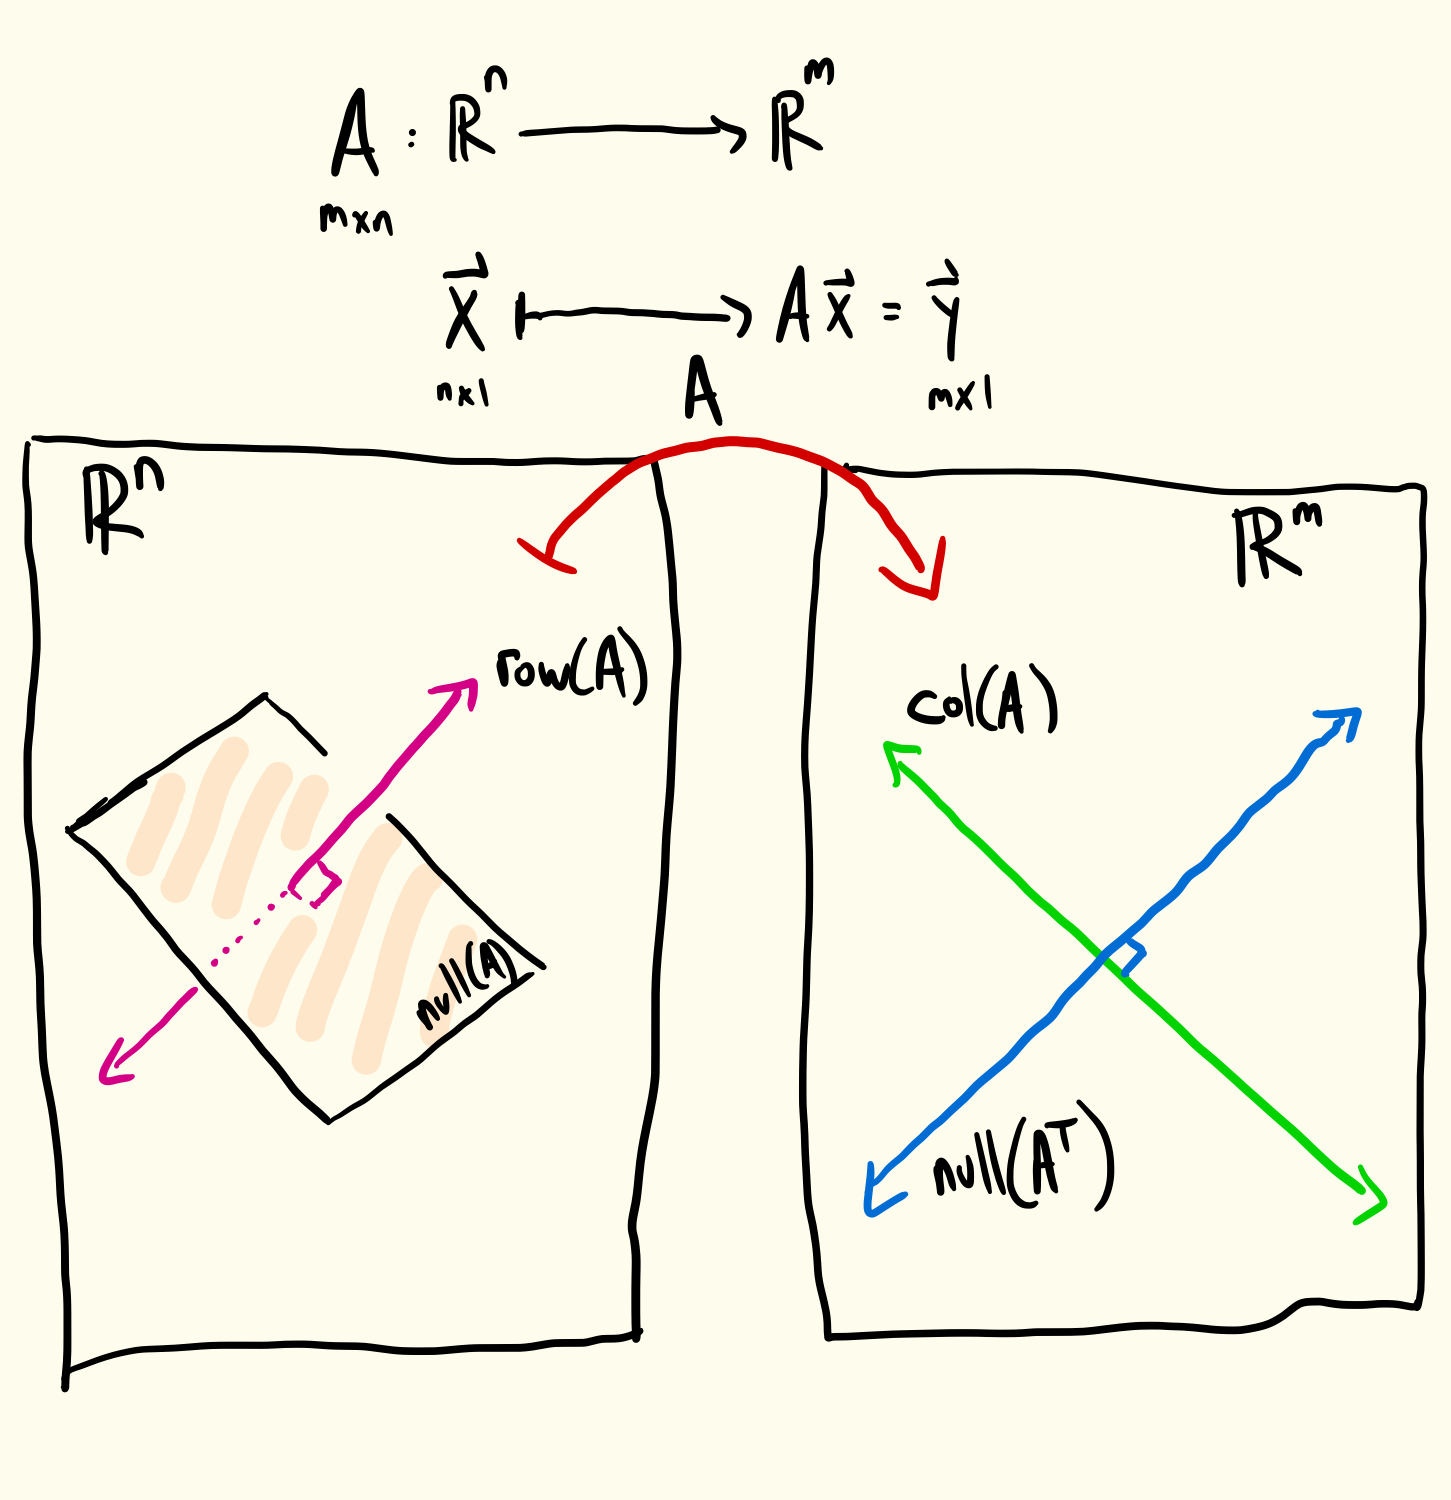
\includegraphics[width=3.5in]{Images/RankNullity}
\]
\end{frame}
\begin{frame}{Example}
Understanding the orthogonal relationship between $\NS(A)$ and $\RS(A)$ allows us in many cases to quickly determine/visualize the one from the other. 
\bspace
Consider the example $A=\begin{bmatrix}[rrr]
1&-1&1\\
1&-1&-1
\end{bmatrix}
$.
\pause Looking at the columns, we see easily that $\rank(A)=2$, which implies that $\nullity(A)=3-2=1$. Since $(1,-1,0)$ is an element of $\NS(A)$ and $\dim(\NS(A))=1$, we must have $\NS(A)=\Span\{(1,-1,0)\}$, a line. 
\bpause
By orthogonality, we conclude that 
\[ \RS(A)=\NS(A)^\perp=\text{(plane perpendicular to $(1,-1,0)$)}. 
\]
\[
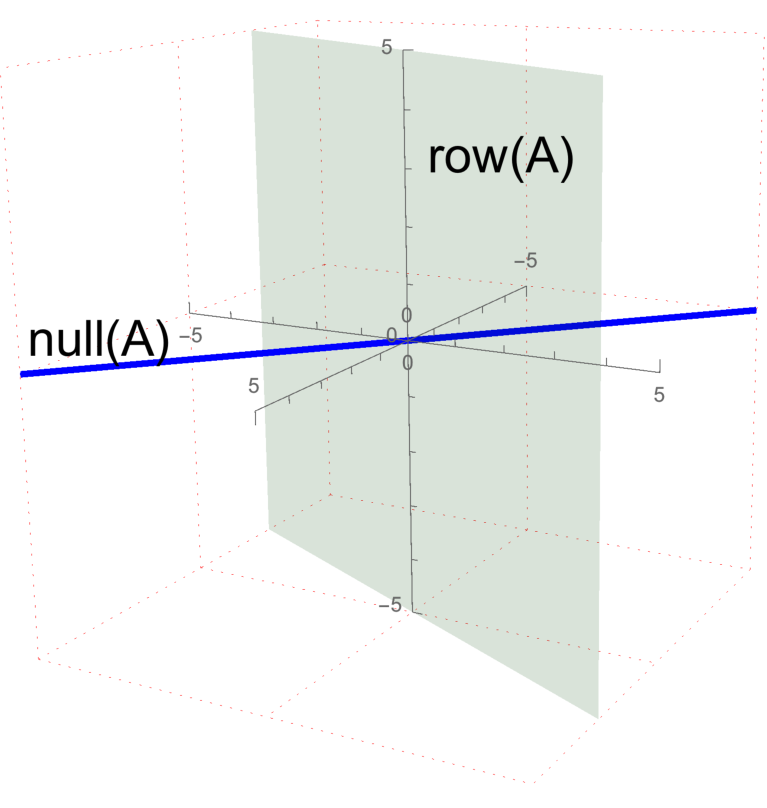
\includegraphics[width=2in]{Images/NullRow}
\]
\end{frame}
\begin{frame}{Orthogonal Projection}
\begin{theorem}[Orthogonal projection theorem]
Let $(V,\langle \ , \rangle)$ be an inner product space, and let $W\subseteq V$ be a \alert{finite-dimensional} subspace. 
\bb[(a)]
\ii (Orthogonal decomposition). 
For all $\boldv\in V$ there is a unique choice of vectors $\boldw\in W$ and $\boldw^\perp\in W^\perp$ such that $\boldv=\boldw+\boldw^\perp$. 

We call this vector expression an {\bf orthogonal decomposition} of $\boldv$, and denote $\boldw=\proj{\boldv}{W}$ and $\boldw^\perp=\proj{\boldv}{W^\perp}$, the {\bf orthogonal projections} of $\boldv$ onto $W$ and $W^\perp$, respectively. 
\pause\ii The orthogonal projection $\boldw=\proj{\boldv}{W}$ is the element of $W$ \alert{closest} to $\boldv$. This means $\norm{\boldv-\proj{\boldv}{W}}\leq\norm{\boldv-\boldw'}$ for any other $\boldw'\in W$. We thus define the distance from $\boldv$ to $W$ as $d(\boldv, W)=\norm{\boldv-\proj{\boldv}{W}}=\norm{\boldw^\perp}$. 
\pause\ii (Orthogonal projection formula). Pick an {\em orthogonal} basis $B=\{\boldv_1,\boldv_2,\dots, \boldv_r\}$ of $W$. 
Then $\ds \proj{\boldv}{W}=\sum_{i=1}^r\frac{\angvec{\boldv,\boldv_i}}{\angvec{\boldv_i, \boldv_i}}\boldv_i$.
\ee
\pause
\begin{comment}
An important consequence of this theorem is that $\proj{\boldv}{W}$ can be uniquely characterized by two distinct properties:

(i) it is the unique element $\boldw$ of $W$ \alert{closest} to $\boldv$

(ii) it is the unique element $\boldw$ of $W$ such that $\boldv-\boldw$ is \alert{orthogonal} to $W$. 
\end{comment}
\end{theorem}
\end{frame}
\begin{frame}{Proof of orthogonal projection theorem}\scriptsize
Pick an {\em orthogonal} basis $B=\{\boldv_1,\boldv_2,\dots, \boldv_r\}$ of $W$ and set $\boldw=\sum_{i=1}^r\frac{\angvec{\boldv,\boldv_i}}{\angvec{\boldv_i, \boldv_i}}\boldv_i$. This is clearly an element of $W$. Next we set $\boldw^\perp=\boldv-\boldw=\boldv-\sum_{i=1}^r\frac{\angvec{\boldv,\boldv_i}}{\angvec{\boldv_i, \boldv_i}}\boldv_i$. 
\bpause
To complete the proof, we must show the following: (A) $\boldw^\perp\in W^\perp$, (B) this choice of $\boldw$ and $\boldw^\perp$ is unique, and (C) $\boldw$ is the closest element of $W$ to $\boldv$. 
\bpause 
\alert{(A)}. For all $i$ we have 
\begin{eqnarray*}
\langle\boldw^\perp,\boldv_i\rangle&=&\langle \boldv-\sum_{i=1}^r\frac{\angvec{\boldv,\boldv_i}}{\angvec{\boldv_i, \boldv_i}}\boldv_i, \boldv_i\rangle\\
\pause&=&\langle \boldv, \boldv_i\rangle-\langle \sum_{i=1}^r\frac{\angvec{\boldv,\boldv_i}}{\angvec{\boldv_i, \boldv_i}}\boldv_i ,\boldv_i\rangle \hspace{9pt} \text{(distr.)}\\
\pause&=&\langle \boldv, \boldv_i\rangle-\frac{\angvec{\boldv,\boldv_i}}{\angvec{\boldv_i,\boldv_i}}\langle\boldv_i,\boldv_i\rangle \hspace{9pt} \text{ (by orthogonality)}\\
\pause&=&0 
\end{eqnarray*}
\pause
\alert{(B)+(C)}. Recall: $\boldw$ satisfies $\boldv=\boldw+\boldw^\perp$, where $\boldw^\perp\in W^\perp$. Now take any other $\boldw'\in W$. Then 
\begin{eqnarray*}
\norm{\boldv-\boldw'}^2&=&\norm{\boldw^\perp+(\boldw-\boldw')}^2
\pause=\norm{\boldw^\perp}^2+\norm{\boldw-\boldw'}^2 \hspace{9pt} \text{ (Pythag. theorem)}\\
\pause&\geq& \norm{\boldw^\perp}^2=\norm{\boldv-\boldw}^2.
\end{eqnarray*}
\pause Taking square-roots now proves the desired inequality. 
Furthermore, we have {\em equality} iff the last inequality is an equality iff $\norm{\boldw''}=\norm{\boldw-\boldw'}=0$ iff $\boldw=\boldw'$. This proves our choice of $\boldw$ is the {\em unique} element of $W$ minimizing the distance to $\boldv$!  
\end{frame}
\begin{frame}
 \begin{corollary}
Let $(V,\angvec{\ , \ })$ be an inner product space, and let $W\subseteq V$ be a finite-dimensional subspace. Then $(W^\perp)^\perp=W$. 
 \end{corollary} 
 \pause
 \begin{proof}
 Clearly $W\subseteq (W^\perp)^\perp$.
 \bspace 
 For the other direction, take $\boldv\in (W^\perp)^\perp$. Using the \alert{orthogonal projection theorem}, we can write $\boldv=\boldw+\boldw^\perp$ with $\boldw\in W$ and $\boldw^\perp\in W^\perp$. We will show $\boldw^\perp=\boldzero$. 
 \bpause 
 Since $\boldv\in (W^\perp)^\perp$ we have $\angvec{\boldv,\boldw^\perp}=0$. Then we have 
 \begin{align*}
  0&=\angvec{\boldv,\boldw^\perp}\\
  &=\angvec{\boldw+\boldw^\perp,\boldw^\perp}\\
  &=\angvec{\boldw,\boldw^\perp}+\angvec{\boldw^\perp,\boldw^\perp} &\text{(since $W\perp W^\perp$)}\\
  &=0+\angvec{\boldw^\perp,\boldw^\perp}
 \end{align*} 
\pause Thus $\angvec{\boldw^\perp,\boldw^\perp}=0$.
\bspace It follows that $\boldw^\perp=\boldzero$, and hence $\boldv=\boldw+\boldzero=\boldw\in W$. 
 \end{proof} 
\end{frame} 
\begin{frame}
 \begin{corollary}
 Let $(V,\angvec{\ , \ })$ be an inner product space, and let $W\subseteq V$ be a finite-dimensional subspace. 
 
 \noindent
 Define $T\colon V\rightarrow V$ as $T(\boldv)=\proj{\boldv}{W}$. Then $T$ is a linear transformation. 
 
 \noindent
 In other words, orthogonal projection onto $W$ defines a linear transformation of $V$. 
 \end{corollary}
 \pause
 \begin{proof}
 We must show that $T(c\boldv_1+d\boldv_2)=cT(\boldv_1)+dT(\boldv_2)$ for all $c,d\in\R$ and $\boldv_1,\boldv_2\in V$.  This is easily shown by picking an orthonormal basis $B=\{\boldv_1,\boldv_2, \dots, \boldv_r\}$ of $W$ and using the formula from the orthogonal projection theorem. 
 \end{proof}
\end{frame}
\begin{frame}{Projection onto lines and planes in $\R^3$}
Let's revisit orthogonal projection onto lines and planes in $\R^3$ passing through the origin. Here the relevant inner product is dot product.  
\begin{block}{Projection onto a line $\ell$}
Any line in $\R^3$ passing through the origin can be described as $\ell=\Span\{\boldv_0\}$, for some $\boldv_0=(a,b,c)\ne 0$. Since this is an orthogonal basis of $\ell$, by the orthogonal projection theorem we have, for any $\boldv=(x,y,z)$ 
\[
\proj{\boldv}{\ell}=\frac{\boldv\cdot \boldv_0}{\boldv_0\cdot\boldv_0}\boldv_0=\frac{ax+by+cz}{a^2+b^2+c^2}(a,b,c)=\frac{1}{a^2+b^2+c^2}\begin{bmatrix}
a^2&ab&ac\\
ab&b^2&bc\\
ac&bc&c^2
\end{bmatrix}\begin{bmatrix}x\\ y\\ z
\end{bmatrix}.
\] 
\pause We have re-derived the matrix formula for orthogonal projection onto $\ell$. 
\end{block}
\end{frame}
\begin{frame}{Projection onto lines and planes in $\R^3$}
Let's revisit orthogonal projection onto lines and planes in $\R^3$ passing through the origin. Here the relevant inner product is dot product.  
\begin{block}{Projection onto a plane $\mathcal{P}$}
Any plane in $\R^3$ passing through the origin can be described with the equation $\mathcal{P}\colon ax+by+cz=0$ for some $\boldn=(a,b,c)\ne 0$. This says precisely that $\mathcal{P}$ is the orthogonal complement of the line $\ell=\Span\{(a,b,c)\}$: i.e., $\mathcal{P}=\ell^\perp$. 
\bpause
From the orthogonal projection theorem, we know that 
\[\boldv=\proj{\boldv}{\ell}+\proj{\boldv}{\ell^\perp}=\proj{\boldv}{\ell}+\proj{\boldv}{\mathcal{P}}.\] 
\pause 
But then
\[
\proj{\boldv}{\mathcal{P}}=\boldv-\proj{\boldv}{\ell}=I \ \boldv-\proj{\boldv}{\ell}=(I-A)\boldv,
\] 
where $A$ is the matrix formula for $\proj{\boldv}{\ell}$ from the previous example. We conclude that   the matrix defining $\proj{\boldv}{\mathcal{P}}$ is 
\[
I-\frac{1}{a^2+b^2+c^2}\begin{bmatrix}
a^2&ab&ac\\
ab&b^2&bc\\
ac&bc&c^2
\end{bmatrix}=
\frac{1}{a^2+b^2+c^2}\begin{bmatrix}
b^2+c^2&-ab&-ac\\
-ab&a^2+c^2&-bc\\
-ac&-bc&a^2+b^2
\end{bmatrix}
\]
\end{block}
\end{frame}
%\begin{frame}{Example: projection onto a plane in $\R^3$}
%\scriptsize
%\alert{Caveat}. In what follows I declare $O=(0,0,0)$ and shamelessly equate a point $P=(x,y,z)\in \R^3$ with its position vector $\overrightarrow{OP}$. 
%
%\bspace
%\vspace{.1in}
%In vector calculus a plane $\mathcal{P}$ \alert{passing through the origin} is defined as the set of points whose coordinate vectors are orthogonal to a given normal vector $\boldn=(a,b,c)$. In our new language, this is equivalent to saying $\mathcal{P}$ is the orthogonal complement to $\ell=\Span\{(a,b,c)\}$, the line defined by $\boldn$. 
%\bpause
%Again, given a point $P=(x,y,z)$ the intuitive idea of ``dropping the perpendicular from $P$ to $\mathcal{P}$" is nothing more than $\proj{(x,y,z)}{\mathcal{P}}$. The orthogonal projection theorem suggests two different means of computing this:
%\bpause
%\alert{(1)}. Compute an \alert{orthogonal} basis for $\mathcal{P}$ and then use the orthogonal projection formula. 
%\bpause
%\alert{(2)} Alternatively, the theorem says $(x,y,z)=\proj{(x,y,z)}{\mathcal{P}}+\proj{(x,y,z)}{\ell}$, and hence 
%\begin{align*}
%\proj{(x,y,z)}{\mathcal{P}}&=(x,y,z)-\proj{(x,y,z)}{\ell}\\
%&=
%\colvec{x\\y\\z}-\frac{1}{a^2+b^2+c^2}\begin{bmatrix}
%a^2&ab&ac\\
%ab&b^2&bc\\
%ac&bc&c^2
%\end{bmatrix}
%\colvec{x\\ y\\ z}\\
%&=\frac{1}{a^2+b^2+c^2}\begin{bmatrix}
%b^2+c^2&-ab&-ac\\
%-ab&a^2+c^2&-bc\\
%-ac&-bc&a^2+b^2
%\end{bmatrix}
%\colvec{x\\ y\\ z}
%\end{align*}
%\end{frame}
%\begin{frame}{Projection onto plane in $\R^3$}
%\[
%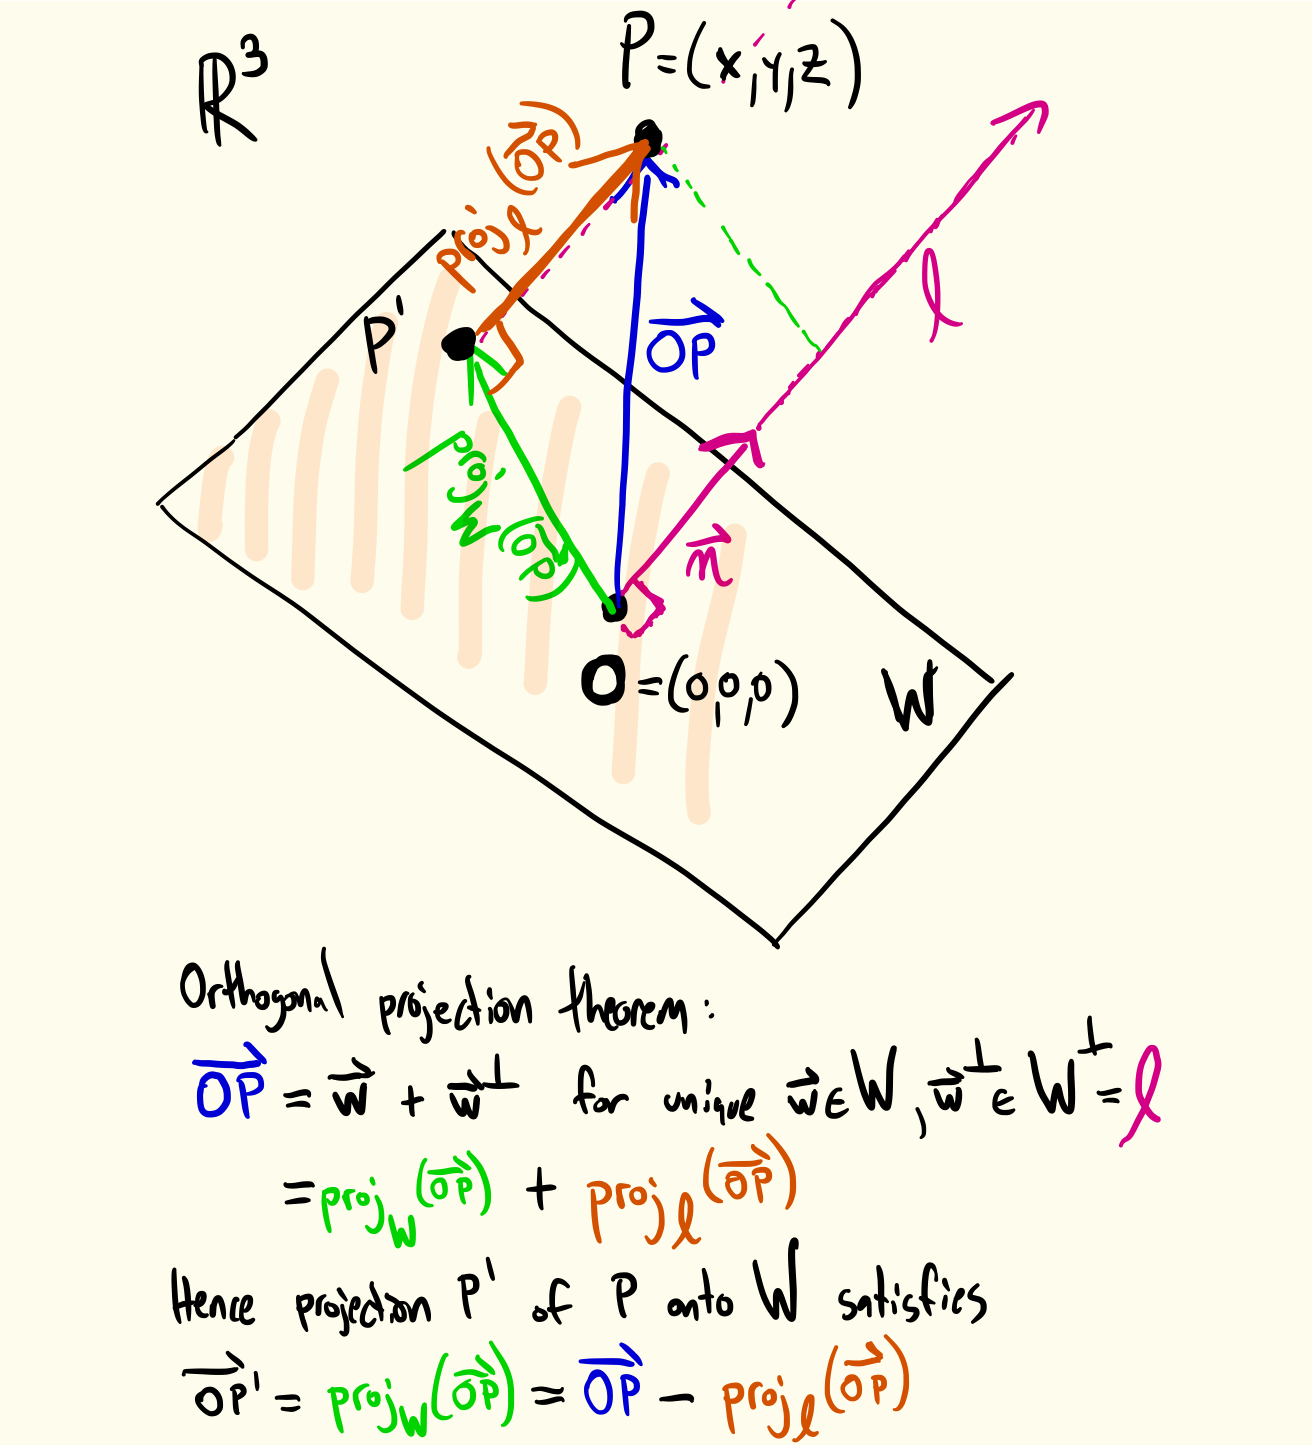
\includegraphics[width=3in]{Images/ProjPlaneDraw}
%\]
%\end{frame}
%\begin{frame}{Example}
%Define $\mathcal{P}: x+y+z=0$: i.e., $\boldn=(1,1,1)$. Let's use the first method in the previous slide to compute the projection of a point $P=(x,y,z)$ onto $\mathcal{P}$. 
%\bpause
%First pick \alert{any orthogonal} basis of $\mathcal{P}$: e.g., $B=\{(1,-1,0), (1,1,-2)\}$. 
%
%Then given $P=(x,y,z)$, the orthogonal projection formula yields 
%{\scriptsize
%\[
%\proj{(x,y,z)}{\mathcal{P}}=\frac{x-y}{2}(1,-1,0)+\frac{x+y-2z}{6}(1,1,-2). 
%\]
%}
%\pause We can express this in terms of matrix multiplication as 
%\[
%\proj{(x,y,z)}{\mathcal{P}}=\frac{1}{3}\begin{bmatrix}[rrr]
%2&-1&-1\\
%-1&2&-1\\
%-1&-1&2
%\end{bmatrix}
%\begin{bmatrix}
%x\\ y\\ z
%\end{bmatrix}.
%\]
%\pause
%\alert{Check}.  We get the same answer using the matrix formula from the previous slide, where we set $(a,b,c)=(1,1,1)$ !!
%\end{frame}
%\begin{frame}{General lines and planes in $\R^3$}
%So how do we proceed if have a line or plane in $\R^3$ that \alert{does not pass through the origin}? 
%\bb
%\pause
%\ii  Find any point $Q=(q_1,q_2,q_3)$ on the line/plane.
%\pause \ii Translate the whole picture by $-Q=(-q_1,-q_2, -q_3)$, which means we replace $P=(x,y,z)$ with $P-Q=(x-q_1,y-q_2,z-q_3)$.
%\pause \ii Apply our formulas from before, replacing $(x,y,z)$ with $(x-q_1,y-q_2,z-q_3)$
%\pause \ii Translate back by adding $Q$ to your answer. 
%\ee
%The result, as you can check, is as follows:
%\bpause
%\alert{Projection onto line}. If $\ell$ is the line passing through $Q=(q_1,q_2,q_3)$ with direction vector $(a,b,c)$, then 
%\[
%\proj{(x,y,z)}{\ell}=\frac{1}{a^2+b^2+c^2}\begin{bmatrix}
%a^2&ab&ac\\
%ab&b^2&bc\\
%ac&bc&c^2
%\end{bmatrix}
%\colvec{x-q_1\\ y-q_2\\ z-q_3}+\colvec{q_1\\ q_2\\ q_3}
%\]
%\bpause
%\alert{Projection onto plane}. If $\mathcal{P}$ is the plane passing through $Q=(q_1,q_2,q_3)$ with normal vector $\boldn=(a,b,c)$, then 
%\[
%\proj{(x,y,z)}{\mathcal{P}}=\frac{1}{a^2+b^2+c^2}\begin{bmatrix}
%b^2+c^2&-ab&-ac\\
%-ab&a^2+c^2&-bc\\
%-ac&-bc&a^2+b^2
%\end{bmatrix}
%\colvec{x-q_1\\ y-q_2\\ z-q_3}+
%\colvec{q_1\\ q_2\\ q_3}
%\]
%\end{frame}
%\begin{frame}{Example}
%\scriptsize
% Define $\mathcal{P}\colon (x-1)+(y-1)+2(z-1)=0$, and let $P=(0,1,5)$. Compute (a) $\proj{(0,1,5)}{\mathcal{P}}$, and (b) the distance from $P$ to $\mathcal{P}$.
%\bpause
%From the equation, we see that $\boldn=(1,1,2)$, and that $Q=(1,1,1)$ is a point in the plane. 
%\bpause
%Using the formula from the previous slide, we compute 
%\[
%\proj{(0,1,5)}{\mathcal{P}}=\frac{1}{6}\begin{bmatrix}
%5&-1&-2\\
%-1&5&-2\\
%-2&-2&2
%\end{bmatrix}
%\colvec{0-1\\ 1-1\\ 5-1\\}+
%\colvec{1\\ 1\\ 1}
%=\colvec{-7/6\\ -1/6 \\ 8/3}
%\]
%\pause
%By definition the distance between $(0,1,5)$ and $\mathcal{P}$ is 
%\[
%d((0,1,5), (-7/6, -1/6, 8/3))=\sqrt{49/36+49/36+49/9}=7\sqrt{6}/6.
%\]
%\pause
%Here is a picture of the situation. The distance from $P$ to $\mathcal{P}$ is the length of the pink normal line. 
%\[
%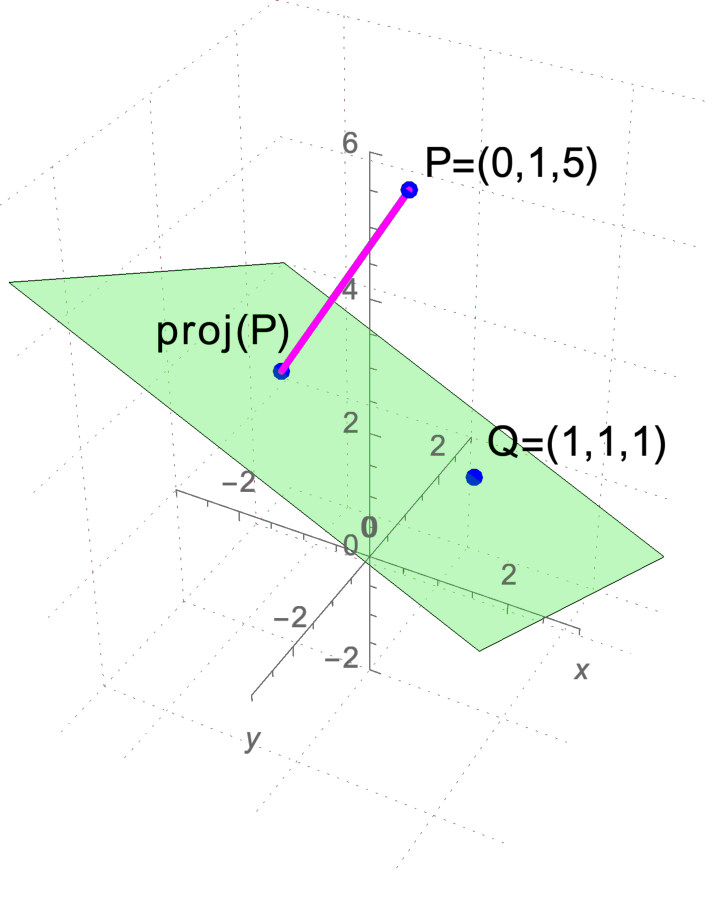
\includegraphics[width=1.5in]{Images/ProjPlane.pdf}
%\]
%
%\end{frame}
\begin{frame}{Example: sine/cosine series}
Let $V=C[0,2\pi]$ with inner product $\langle f, g\rangle=\int_0^{2\pi}f(x)g(x) \, dx$. 

We have seen that the set
\[
B=\{1, \cos(x),\sin(x),\cos(2x),\sin(2x), \dots , \cos(nx),\sin(nx)\} 
\] 
is orthogonal. Thus $B$ is an orthogonal basis of $W=\Span(B)$, which we might describe as the space of {\bf trigonometric polynomials of degree at most $n$}. 
\bpause
Given an arbitrary function $f(x)\in C[0,2\pi]$, its orthogonal projection onto $W$ is the function 
\[
\hat{f}(x)=a_0+a_1\cos(x)+b_1\sin(x)+a_2\cos(2x)+b_2\sin(2x)+\cdots +a_n\cos(nx)+b_n\sin(nx),
\]
where 
\[
a_0=\frac{1}{2\pi}\int_0^{2\pi} f(x) \ dx, \ a_j=\frac{1}{\pi}\int_0^{2\pi}f(x)\cos(jx)\, dx, \ b_k=\frac{1}{\pi}\int_0^{2\pi}f(x)\sin(kx)\, dx.
\]
\pause
The projection theorem tells us that $\hat{f}$ is the ``best" trigonometric polynomial approximation of $f(x)$ (of degree at most $n$), in the sense that for any other sinusoidal $g\in W$, $\left\vert\left\vert f-\hat{f}\right\vert\right\vert\leq \norm{f-g}$.  
\bpause 
This means in turn 
\[
\int_0^{2\pi} (f-\hat{f})^2\, dx\leq \int_0^{2\pi} (f-g)^2 \, dx.
\]
\end{frame}
\begin{frame}{Example: least-squares solution to $A\boldx=\boldy$}
Often in applications we have an $m\times n$  matrix $A$ and vector $\boldy\in\R^m$ for which the matrix equation 
\[
A\boldx=\boldy
\]  
has no solution. In terms of fundamental spaces, this means simply that $\boldy\notin \CS(A)$. Set $W=\CS(A)$.     
\bpause
In such situations we speak of a \alert{least-squares} solution to the matrix equation. This is a vector $\hat{\boldx}$ such that $A\hat{\boldx}=\hat{\boldy}$, where $\hat{\boldy}=\proj{\boldy}{W}$. Here the inner product is taken to be the dot product. 

Note: the equation $A\hat{\boldx}=\hat{\boldy}$ is guaranteed to have a solution since $\hat{\boldy}=\proj{\boldy}{W}$ lies in $\CS(A)$. 

\pause
The vector $\hat{\boldx}$ is called a least-square solutions because its image $\hat{\boldy}$ is the element of $\CS(A)$ that is ``closest" to $\boldy$ in terms of the dot product. 
\bspace 
Writing $\boldy=(y_1,y_2,\dots,y_n)$ and $\hat{\boldy}=(y_1',y_2',\dots, y_n')$, this means that $\hat{\boldy}$ minimizes the distance 
\[
\norm{\boldy-\hat{\boldy}}=\sqrt{(y_1-y_1')^2+(y_2-y_2')^2+\cdots +(y_n-y_n')^2}.
\]  
\end{frame}
\begin{frame}{Least-squares example (curve fitting)}
Suppose we wish to find an equation of a line $y=mx+b$ that best fits (in the least-square's sense) the following $(x,y)$ data points: $P_1=(-3,1), P_2=(1,2), P_3=(2,3)$. 

\pause
Then we seek $m$ and $b$ such that 
\begin{align*}
1&=m(-3)+b\\
2&=m(1)+b\\
3&=m(2)+b,
\end{align*} 
or equivalently, we wish to solve 
$
\begin{bmatrix}[rr]
-3&1\\ 1&1\\ 2&1
\end{bmatrix}
\begin{bmatrix}
m \\ b
\end{bmatrix}
=\begin{bmatrix}
1\\ 2\\ 3
\end{bmatrix}$. 
\bpause
This equation has no solution as $\boldy=(1,2,3)$ does no lie in $W=\CS(A)=\Span(\{(-3,1,2),(1,1,1)\}$. So instead we compute $\hat{\boldy}=\proj{\boldy}{W}=(13/14,33/14,38/14)$. (This was not hard to compute as conveniently the given basis of $W$ was already orthogonal!)  
\bpause
Finally we solve $A\begin{bmatrix}
m\\ b
\end{bmatrix}=\hat{\boldy}$, getting $m=5/14$, $b=28/14=2$. Thus $y=\frac{5}{14}x+2$ is the line best fitting the data in the least-squares sense. 
\end{frame}
\begin{frame}{Least-squares example contd.}
In what sense does $y=\frac{5}{14}x+2$ ``best" fit the data? 
\[
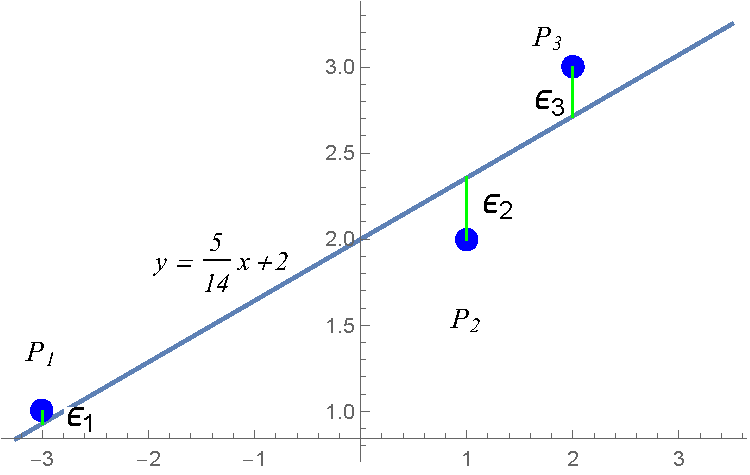
\includegraphics[width=2in]{Images/LeastSquares}
\]
Let $\boldy=(1,2,3)=(y_1,y_2,y_3)$ be the given $y$-values of the points, and $\hat{\boldy}=(y_1',y_2',y_3')$ be the projection we computed before. In the graph the values $\epsilon_i$ denote the vertical difference $\epsilon_i=y_i-y_i'$ between the data points, and our fitting line. 
\bpause 
The projection $\hat{\boldy}$ makes the error $\norm{\boldy-\hat{\boldy}}=\sqrt{  \epsilon_1^2+\epsilon_2^2+\epsilon_3^2}$ as small as possible. 

This means if I draw {\em any other line} and compute the corresponding differences $\epsilon_i'$ at the $x$-values -3, 1 and 2, then we have 
\[
\epsilon_1^2+\epsilon_2^2+\epsilon_3^2\leq (\epsilon_1')^2+(\epsilon_2')^2+(\epsilon_3')^2
\]  
\end{frame}
\begin{frame}{Finding least squares solutions}
As the last example illustrated, one method of finding a least-squares solution $\boldx$ to $A\boldx=\boldy$ is to 
first produce an orthogonal basis for $\CS(A)$, then compute $\hat{\boldy}=\proj{\boldy}{\CS(A)}$, and then use GE to solve $A\boldx=\hat{\boldy}$. 

\bpause
Alternatively, it turns out (through a little trickery) that $\hat{\boldy}=A\boldx$, where $\boldx$ is a solution to the equation 
\[
\boxed{A^TA\boldx=A^T\boldy}.
\]
This solves us the hassle of computing an orthogonal basis for $\CS(A)$; to find a least-squares solution $\boldx$ for $A\boldx=\boldy$, we simply use GE to solve the boxed equation. (Some more trickery shows a solution is guaranteed to exist!) 
\bpause
\alert{Example}. In the previous example we were seeking a least-squares solution $\boldx=\colvec{m\\ b}$ to $A\boldx=\boldy$, where 
$
A=\begin{bmatrix}[rr]
 -3&1\\
 1&1\\
 2&1
\end{bmatrix} , \boldy=\colvec{1\\2\\3}
$.

The equation $A^TA\boldx=A^T\boldy$ is thus 
\[
\begin{bmatrix}
14&0\\
0&3
\end{bmatrix}
\boldx=
\colvec{5\\ 6} 
\]
As you can see, $\boldx=\colvec{m\\ b}=\colvec{5/14\\ 2}$ is a least-squares solution, just as before
\end{frame}
\end{document}